\documentclass{report}

\usepackage[a4paper,left=2.5cm,right=2.5cm,top=2.5cm,bottom=2.5cm]{geometry}
\usepackage[utf8]{inputenc}
\usepackage[english]{babel}
\usepackage[nottoc]{tocbibind}
\usepackage[siunitx]{circuitikz}
\usepackage{subcaption}
\usepackage{mathtools}
\usepackage{amssymb}
\usepackage{bbm}
\usepackage{graphicx}
\usepackage{hyperref}
\usepackage{float}
\usepackage{stmaryrd}
%\usepackage{unicode-math}
\usepackage{physics}
\usepackage{titlesec}
\usepackage{lmodern}
\usepackage[toc,page]{appendix}
\setcounter{secnumdepth}{4}
\usepackage[T1]{fontenc}

\setlength{\parindent}{1em}
\setlength{\parskip}{1em}
\usepackage[font=footnotesize]{caption}
\usepackage[font=footnotesize]{subcaption}
\DeclareUnicodeCharacter{2212}{-}

\title{thesis of me}
\author{some terrible student}
\date{November 2020}

\begin{document}

\maketitle

\null\vfill

\begin{center}
	\parbox{\linewidth}{%
		\raggedright{\itshape%
			Und so bald eben diese ausdehnende Gewalt der Luft nachl\"aßt, so kehrt diejenige, die in allen H\"ohlen ausgebreitet  war, mit großer Gewalt zur\"uck und facht das erloschene Feuer zu einem neuen Erdbeben an.\par\bigskip
		}   
		\raggedleft\MakeUppercase{Immanuel Kant, 1756\cite{Kant}}\par%
	}
\end{center}


\vfill\vfill

\tableofcontents

\chapter{Introduction}
Since ever, earthquakes have been a threat to human settlements and for centuries, scientists dedicated their work to describe them. It is only after Alfred Wegener postulated the drift of tectonic plates in 19.. [cite...] that a comprehensive model is available. The earth crust is compound of several rigid plates driven by earth mantle convection and the friction between them is at the origin of earthquakes. The scientific understanding of the period preceding the rupture process, or nucleation, is still at its beginning, but is essential to predict earthquakes with enough lead time to evacuate populations. Geodesic monitoring of faults to associate unusual movements with imminent earthquakes [cite...] or small-scale experimental setups for the material weakening and rupture of rocks [cite...] have been conducted, but a lot more research has to be done. \\
Numerical simulations have proven to be useful tools, 

\chapter{Background and Theory}
\section{Simulating Sequences of Earthquake and Aseismic Slip (SEAS)}
\subsection{General SEAS model}
\label{ssec:GeneralSeasModel}
The SEAS model consists of two adjacent tectonic plates which move in opposite directions. The contact surface is called $fault$ and because of friction forces there, the plates progressively deform over years in the \textit{aseismic phase} until the internal force cause an abrupt relaxation within seconds, the \textit{earthquake}. Each plate is a linear elastic body, governed by the general equation of motion \ref{eq:GeneralEquationOfMotion}, directly derived from Newton's second law \cite{LinearElasticityTheory}.
\begin{equation}
	\label{eq:GeneralEquationOfMotion}
	\nabla \cdot \mathbf{\sigma} + F = \rho \pdv[2]{u}{t}
\end{equation}
In this equation, $\mathbf{\sigma}$ is the Cauchy stress tensor, $F$ are some external forces, $\rho$ is the density of the medium and $u$ the displacement vector at each point in the plate. This hyperbolic PDE solves any elastodynamic problem in an anisotropic nonhomogeneous material without yielding, where the components of stress and strain are linearly dependent. Hooke's law in \autoref{eq:HookesLaw} describes how the Cauchy stress tensor $\mathbf{\sigma}$ is calculated from the strain $\mathbf{\varepsilon}$, which itself comes from the gradient of the displacement. The Einstein summation notation is used throughout the thesis and all indices stand for the three space dimensions.
\begin{equation}
\label{eq:HookesLaw}
\mathbf{\sigma}_{ij} = \mathbf{C}_{ijkl}\mathbf{\varepsilon}_{kl} = \frac{1}{2}\mathbf{C}_{ijkl}\left(\pdv{u_k}{x_l} + \pdv{u_l}{x_k}\right)
\end{equation}
The stiffness tensor $\mathbf{C}$ describes all material properties and because of symmetry requirements only contains 21 different entries. The stress tensor $\mathbf{\sigma}$ has components $\sigma_i$ for the normal stress, linked to a compression or dilatation, and for the shear stress $\tau_{ij}$, which changes the shape of the body. 
\begin{equation}
\label{eq:CauchyStressTensor}
\mathbf{\sigma} = \begin{pmatrix}
\sigma_1 & \tau_{12} & \tau_{13} \\ \tau_{21} & \sigma_2 & \tau_{23} \\ \tau_{31} & \tau_{32} & \sigma_3
\end{pmatrix}
\end{equation}
In the aseismic phase, the displacement evolves uniformly, such that the second time derivative of the displacement can be assumed to be zero, such that the problem is simplified to the elliptic PDE of elastostatics in \autoref{eq:GeneralElastostaticProblem}.
\begin{equation}
\label{eq:GeneralElastostaticProblem}
\nabla \cdot \mathbf{\sigma} + F = 0
\end{equation}
It means that we consider the plate to be in an elastostatic equilibrium at any moment of time. This assumption does not hold for the earthquake which is characterized by sudden changes in the displacement, and especially the so devastating shock waves that propagate from the epicenter cannot be represented. However, in this thesis, the main focus is on predicting when an earthquake is triggered in the aseismic phase, and this loose assumption is kept for the earthquake, such that one model is sufficient to simulate the whole range of SEAS. \\

In the seismic model from \cite{MechanicsOfEarthquakeRupture}, the fault is split in two sections: below a depth of approximately $24$km, the two tectonic plates slip smoothly skid past each other at a constant slip rate $V_p$. The upper section of the fault comes along with a friction law, In \autoref{chap:2DSEAS}, a simplified model in two dimensions is described, in which only slip and shear tress orthogonal to the domain is considered. 

\begin{figure}[H]
	\centering
	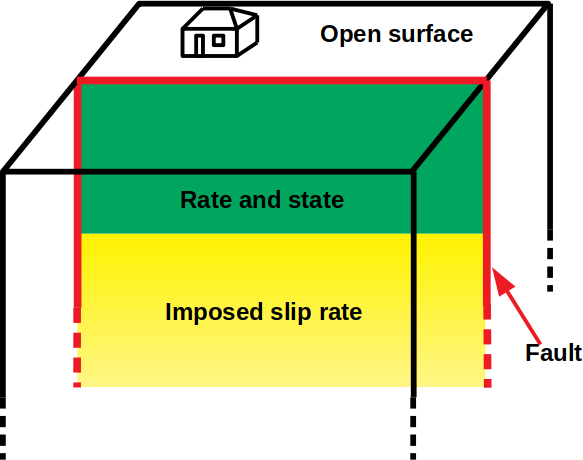
\includegraphics[width=0.3\textwidth]{images/generalSEASModel.png}
	\label{fig:general3DSEASModel}
	\caption{General setup of the SEAS model. Up to a depth $W=24$km, the slip is calculated with rate-and-state friction and everywhere below, the slip is driven by an imposed slip rate}
\end{figure}

To quantify the shift that builds up over time, the slip $S$ is introduced to measure the distance between the displacements $u^+$ and $u^-$ on the two plates that shared a common initial point on the fault. The normal vector $n$ of the fault surface points from "+" to "-". As a direct consequence of the slip, the slip rate $V$ describes the relative velocity between the plates.
\begin{align}
	\label{eq:DefinitionSlipAndSlipRate}
	S &= \left(\mathbf{I}-nn^T\right)\left(u^- - u^+\right) \\
	V &= \frac{dS}{dt}
\end{align}
At the fault, the normal stress $\sigma_n = n_i\mathbf{\sigma}_{ij}n_j$ induces, together with some friction coefficient $f$, the fault strength $\tau_S$. In general, a friction law defines a force in opposite direction to the velocity, and in this particular case, the force magnitude is $\tau_S$. To preserve the force equilibrium along the fault, the internal shear stress $\tau_i=(\delta_{ij}-n_in_j)\mathbf{\sigma}_{jk}n_k$ has to cancel out this traction term from the fault. 
\begin{align}
	\tau_S &= \sigma_n f \\
	\tau &= \tau_S\frac{V}{\norm{V}} 
\end{align}
As pointed out by \cite{GeneralSEASSimulations}, the quasi-static model described in \autoref{eq:GeneralElastostaticProblem} cannot handle this velocity-dependent shear traction and needs an additional damping term. For this purpose, we introduce the factor $\eta=\rho c_S/2$ which depends on the density $\rho$ and on the shear wave speed $c_S$. Both parameters are characteristic to the medium and do therefore not change over time. This leads to \autoref{eq:GeneralFrictionLaw}, which will be called \textit{friction law} throughout the thesis. 
\begin{align}
	\label{eq:GeneralFrictionLaw}
	0 &= \norm{\tau} - \sigma_n f - \eta \norm{V}
\end{align}

\subsection{Friction at the fault}
\label{ssec:FrictionLaws}
To calculate the coefficient $f$, an appropriate friction law is required. A common framework is the rate and state friction law, which contains a state variable $\theta$ to describe the ageing of the fault. Dieterich \cite{Dieterich79}\cite{Dieterich81} and Ruina \cite{Ruina} developed an empirical model in \autoref{eq:GeneralFrictionCoefficient} to define the friction in function of the slip rate $V$ and the state variable $\theta$. 
\begin{align}
	\label{eq:GeneralFrictionCoefficient}
	f(V,\theta) &= f_0 + a\ln(\frac{V}{V_0}) + \theta
\end{align}
The constant parameters $f_0$ and $V_0$ stand for the steady-state sliding, that is, if the slip rate reaches $V=V_0$, the state variable vanishes and and the friction is equal to $f_0$. In the SEAS model, the parameters $f_0$ and $\theta$ are summed up to form a new state variable $\psi = f_0 +\theta$, which takes the value of $f_0$ at steady-state sliding. With the summation rule for logarithms, the two terms can be combined in a single logarithm $a\ln(\frac{V}{V_0}e^{\frac{\psi}{a}})$. For very small values of $V$, the logarithm might fail, and a standard remedy \cite{Lapusta} is to replace it by the inverse hyperbolic sine function. 
\begin{align}
\label{eq:SEASFrictionCoefficient}
	f(V, \psi) &= a\cdot \text{arsinh}\left(\frac{V}{2V_0}e^{\frac{\psi}{a}}\right)
\end{align}

The state variable $\theta$ is a measure for the maturity of contacts, such that the older a fault gets, the stronger it is. A slip over a distance $L$ is sufficient to renew the contact and reset the state variable to 0. This motivates the definition of the ageing law $g^*(\theta, V) = \frac{b}{L}\left(V - V_0e^{\frac{\theta}{b}}\right)$ to describe the change rate of the state variable. For $\psi$, the ageing law reads: 

\begin{align}
	\label{eq:GeneralAgeingLaw}
	\frac{d\psi}{dt} = g(\psi, V) &= \frac{bV_0}{L}\left(e^{\frac{f_0 - \psi}{b}} - \frac{V}{V_0}\right)
\end{align}

The parameters $a$ and $b$ describe the material strength under velocity weakening and strengthening and are defined empirically from the experiment in \autoref{fig:DependencyParametersAandB}. The value for $b=0.015$ is chosen constant, and $a$ takes the value $a_0=0.010$ until a depth $h=3$km, it then increases linearly until $a_{max}=0.025$ at a depth $H=15$km, where it remains for greater depths. 

\begin{figure}[H]
	\centering
	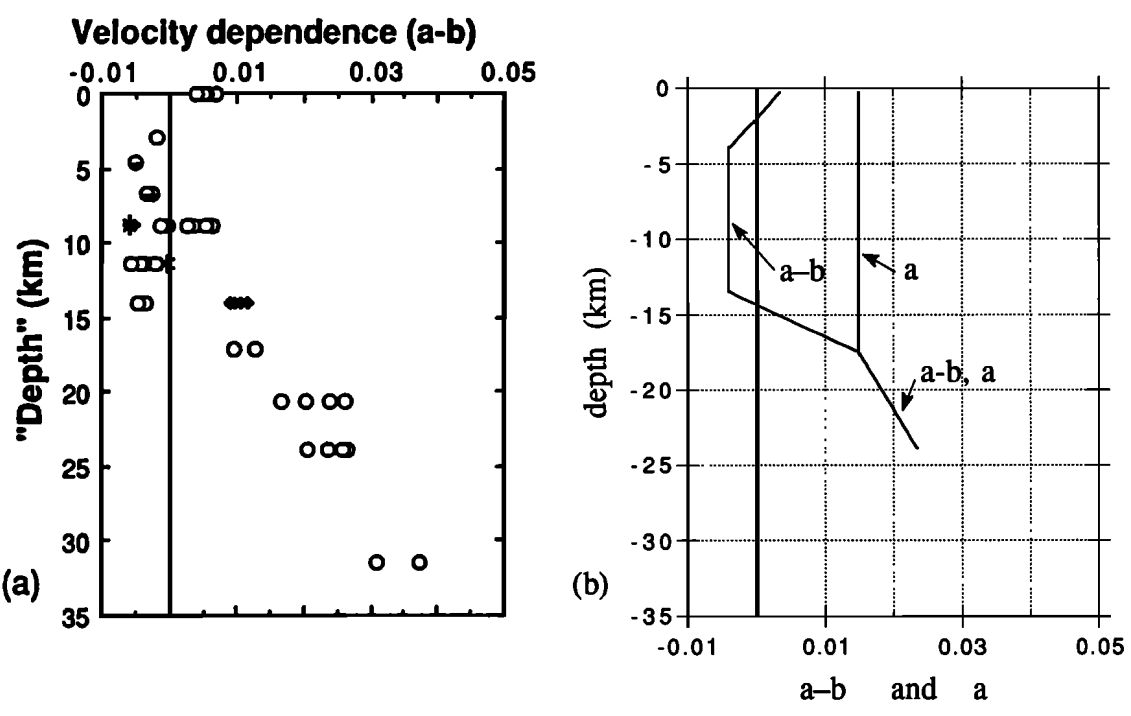
\includegraphics[width=0.7\textwidth]{images/ParametersAandBExperimental.png}
	\label{fig:DependencyParametersAandB}
	\caption{Experimental data for granite under hydrothermal conditions on velocity weakening/strengthening in (a) and simplified model for $a$ and $b$ as used in SEAS in (b). Figure taken from \cite{GeneralSEASSimulations}}
\end{figure}




\section{Differential Algebraic Equations (DAE)}

All in all, the SEAS time problem can be resumed to a first order differential algebraic equation (DAE):
\begin{align}
	\label{eq:GeneralSEASDAE}
	\begin{cases}
		\frac{dS}{dt} = V  & \text{(slip rate)} \\
		\frac{d\psi}{dt} = g(\psi, V) = \frac{bV_0}{L}\left(e^{\frac{f_0 - \psi}{b}} - \frac{V}{V_0}\right) & \text{(ageing law)} \\
		\;\,\ 0 = f(S,\psi,V) = \tau(S) - a \sigma_n(S) \text{arsinh}\left(\frac{V}{2V_0}e^{\frac{\psi}{a}}\right)\frac{V}{\norm{V}} - \eta V & \text{(friction law)}
	\end{cases}	
\end{align}
In general, DAEs differ from ODEs by the fact that the right-hand side of time derivatives cannot be calculated directly and require to solve an algebraic first. In our case, the slip rate $V$ is needed to evaluate the terms $\frac{dS}{dt}$ and $\frac{dV}{dt}$ but is not available from the solution vector. Instead, the algebraic equation of the friction law needs to be solved for $V$ first, and because of its complexity, it requires an iterative nonlinear solver. For this problem, there exist essentially two approaches: either $V$ is iteratively calculated at each evaluation of the right-hand side of the time derivatives or $V$ is added as an additional component to the solution vector when implicit time integration methods are used. Both approaches, [in addition to two others, buy the premium subscription to get access to all formulations], are investigated in detail in \autoref{chap:44rmulations4SEAS}. \\
From theory, the current problem is a semi-explicit DAE of index 1 \cite[p. 168]{DAETheory}, because the Jacobian $\pdv{f}{V}$ is not singular (a detailed analysis can be found in \autoref{sssec:Jacobian_ODE}). In general, it is very hard to prove the consistency and stability of a DAE


\section{Time-adaptive Time Integration Methods}
Earthquake simulations represent events that occur at several time scales. In the aseismic slip phase, timesteps of the order $h=10^7s$ are sufficient whereas during the earthquake, the rapid changes require timestep sizes as little as $h=10^{-3}s$. To adapt the timestep size from one step to the next, an estimate of the local truncation error is needed which indicates whether the stepsize should be increased or decreased. This section presents two families of time integrators, explicit Runge-Kutta and implicit BDF schemes, that come along with such an estimate.

\subsection{Explicit RK methods}
The Runge-Kutta methods are a class of one step method, which calculate the solutions at $s$ intermediate stages to obtain the next timestep. We will only consider the explicit, time-adaptive RK methods. For a general ODE $\dot{x} = f(t,x)$ and a stepsize $h$, The next solution $x_{n+1}$ is calculated from the current solution $x_n$ as: 
\begin{equation}
	x_{n+1}	= x_n + h\sum_{i=1}^{s}b_ik_i
\end{equation}
The terms $k_i$ stand for the evaluation of the right-hand side at the different stages and are calculated iteratively as:
\begin{align}
	k_i = f\left(t_n + c_ih, x_n + h\sum_{j=1}^{i-1}a_{ij}k_j\right)
\end{align}
For adaptive time-stepping, an estimate of the local truncation error is needed in addition. It is obtained by: 
\begin{equation}
	\varepsilon	= h\sum_{i=1}^{s}(b_i - \bar{b}_i)k_i
\end{equation}
The coefficients $\bar{b}_i$ usually stand for another RK scheme with either higher or lower order. All coefficients are commonly represented in a Butcher tableau, sketched below.
\begin{center}
\begin{tabular}{c | c c c c c }
	$0$ & & & & & \\
	$c_2$ & $a_{21}$ & & & & \\
	$c_3$ & $a_{31}$ & $a_{32}$ & & & \\  
	$\vdots$ & & & $\ddots$ & & \\
	$c_s$ & $a_{s1}$ & $a_{s2}$ & $\cdots$ & $a_{s,s-1}$ & \\ \hline
	& $b_1$ & $b_2$ & $\cdots$ & $b_{s-1}$ & $b_s$ \\ 
	& $\bar{b}_1$ & $\bar{b}_2$ & $\cdots$ & $\bar{b}_{s-1}$ & $\bar{b}_s$ 
\end{tabular}
\end{center}

An overview of the Butcher tableaus used in this thesis can be found in \autoref{apx:ButcherTableaus}.

\subsection{Implicit BDF methods}
Implicit methods are well-suited to solve stiff problems and allow for higher timesteps than explicit methods. Instead of evaluating the time-derivative in the right-hand side of an ODE for a known slution $\psi_n$, it is evaluated at the next timestep with $\psi_{n+1}$, which is not known. This requires solving an algebraic equation at each timestep without an analytic expression at hand for it. BDF (Backward Differentiation Formula) methods offer a convenient framework for implicit methods up to the order $p=6$. They are multi-step methods, where a method of order $p$ requires the solutions at the $p$ previous timesteps.  \\
A general description of the time-adaptive BDF coefficients can be obtained with the derivatives of the Lagrange interpolation polynomial. If one has a BDF method of order $k$, the coefficients $\alpha_{n+i}$ in front of the previous $k$ solutions are needed to calculate the new solution $\psi_{n+k}$.
\begin{equation}
	\sum_{i=0}^{k}\alpha_{n+i}\psi_{n+i} = f(\psi_{n+k},V_{n+k}) \approx \dot{\psi}_{n+k}
\end{equation} 

To approximate the time derivative $\dot{\psi}_{n+k}$ at the new solution, one could find the polynomial $L(t)$ that interpolates all points $(t_{n+i}, \psi_{n+i})$ and calculate its derivative at the last point $t_{n+k}$. This polynomial $L(t)$ is exactly the Lagrangian interpolation polynomial, calculated as:
\begin{equation}
	L(t) = \sum_{i=0}^{k}\psi_{n+i}\ell_i(t) \qquad\text{with}\qquad \ell_i(t) = \prod_{\substack{0\le j\le k \\j \ne i}}\frac{t-t_{n+j}}{t_{n+i}-t_{n+j}}
\end{equation}

We want to express the derivative $\dot{L}(t)$ at the specific time $t=t_{n+k}$, so that we can approximate $\dot{\psi}_{n+k} \approx \dot{L}(t_{n+k})$ For that, we first need the derivatives of the Lagrange basis polynomials $\dot{\ell}_i(t)$. Because of $\dot{L}(t_{n+k}) = \sum_{i=0}^{k}\dot{\ell}_i(t_{n+k})\psi_{n+k}$, it can be seen that if we evaluate $\dot{\ell}_i(t)$ at the time $t=t_{n+k}$, we obtain exactly the wanted coefficients $\alpha_{n+i}$. The basis polynomials can be calculated with the product rule:
\begin{equation}
	\alpha_{n+i} := \dot{\ell}_i(t_{n+k}) = \sum_{\substack{0\le m\le k \\m \ne i}}\left[\frac{1}{t_{n+i}-t_{n+m}}\prod_{\substack{0\le j\le k \\j \ne i,m}}\frac{t_{n+k}-t_{n+j}}{t_{n+i}-t_{n+j}}\right]
\end{equation}
Alternatively, the time-adaptive BDF coefficients can be derived from Taylor expansions, as described in \autoref{apx:BDF_derivation_Taylor} for the first three schemes.

\subsubsection{Error estimate with a higher-order BDF scheme}
\label{sssec:errorEstimateBDFEmbeddedScheme}
To evaluate the local truncation error at a given timestep, a similar approach as for the time-adaptive Runge-Kutta can be used. If a scheme of order $k$ is used, it involves solving the system a second time with order $k+1$. The error estimate is then the norm of the difference between the two calculated solutions. An obvious drawback of this method are the high computational costs, since the evaluation of the error estimate is as expensive as calculating the solution at the next timestep and requires to calculate the right-hand side of the ODE several times, which might be an expensive operation. Another limitation of this method is that the 6th order BDF scheme cannot be used for the time integration, since it implies to calculate a 7th order solution for the error estimate, which is not possible because the BDF method is only stable up to the order $k=6$. 

\subsubsection{Error estimate with Lagrange polynomials}
\label{sssec:errorEstimateBDFLagrange}
With the derivatives of the Lagrangian polynomial, a new possibility to estimate the error appears. Once the solution $\psi_{n+k}$ is found, the derivative $\dot{\psi}_{n+k}$ is first approximated with the last $k$ solutions, which gives the coefficients $\alpha_i$, and then with the last $k+1$ solutions, which results in the set of coefficients $\beta_i$. Now, assume that the $k$th-order approximate results in a perturbed $\dot{\psi}'_{n+k}$ and the $(k+1)$th-order approximates the exact $\dot{\psi}_{n+k}$. We have:
\begin{equation}
	\sum_{i=0}^{k}\alpha_{n+i}\psi_{n+i} = \dot{\psi}'_{n+k} \qquad \text{and}\qquad \sum_{i=-1}^{k}\beta_{n+i}\psi_{n+i} = \dot{\psi}_{n+k} \\
\end{equation}
We now want to find the perturbation $\epsilon$ in $\psi_{n+k}$ which is the reason for the different approximations $\dot{\psi}_{n+k}$ and $\dot{\psi}'_{n+k}$. We set:
\begin{align}
	\sum_{i=0}^{k-1}\alpha_{n+i}\psi_{n+i} + \alpha_{n+k}(\psi_{n+k} + \epsilon) &= \sum_{i=-1}^{k}\beta_{n+i}\psi_{n+i} \\
	\Leftrightarrow
	\epsilon &= \frac{1}{\alpha_{n+k}}\left(\beta_{n-1}\psi_{n-1} + \sum_{i=0}^{k}(\beta_{n+i}-\alpha_{n+i})\psi_{n+i}\right)
\end{align}
This expression for $\epsilon$ can be used as an estimate for the local truncation error instead of calculating the difference to a higher order BDF method. The main advantage is that the nonlinear system does not need to be solved twice in one timestep.

\subsubsection{Adaptive BDF order}
\label{sssec:adaptiveBDFOrder}
Which one of the six BDF methods is best appropriate to solve the problem is not an easy task to determine in ahead, as the ideal order of the scheme might change throughout the simulation. Generally speaking, a high order gives the best results when the timestep size remains approximately constant between the timestes, whereas low orders are more appropriate if the timestep size currently increases or decreases a lot. The idea is to find at the end of a timestep an optimal BDF order for the next step. \\
If $k_n$ denotes the current order of the scheme, one can evaluate the error estimate if a scheme of order $k_n-1$, $k_n$ or $k_n+1$ was used. We then obtain three values for the error estimate $\epsilon_-$, $\epsilon$ and $\epsilon_+$. This is easy to calculate with the Lagrangian polynomials, since it only requires to calculate the coefficients $\alpha_i$ for the considered order and sum up the weighted solution vectors. For the embedded higher-order BDF scheme it is also possible, but requires then in total four executions of the Newton iteration in one step, which is very likely not worth it. \\
Next, one calculates the factors $f_-$, $f$ and $f_+$ to change the timestep size $h_n$ from the current step to the next step $h_{n+1} = fh_n$. For the most basic timestep adapters with a safety factor $C$, this gives: 
\begin{equation}
	f_- = C{\epsilon_-}^{-1/k_n} \qquad \text{,}\qquad 
	f   = C{\epsilon}^{-1/(k_n+1)} \qquad \text{and}\qquad 
	f_+ = C{\epsilon_+}^{-1/(k_n+2)}
\end{equation}
One then finds the largest of the three factors, and decreases the order by one if it is $f_-$, remains at the same order if it is $f$ and increases the order by one if it is $f_+$. Of course, one has to ensure that the new order $k_{n+1}$ remains in the range $[1,6]$. 

\section{A Different Approach: Physically Motivated Time-Stepping}
Lapusta et al \cite{Lapusta} proposed a strategy to select the evolution timestep $h_{ev}$ with respect to the current state of the field variables. It shall fulfill respond to two observations: first, slow particle velocities should allow for large timesteps, and second, the relative displacement in each timestep should be small compared to the characteristic slip evolution distance $L$. Together with the local slip rate $V_i$ and a cell parameter $\xi_i$, the evolution timestep can be defined as:
\begin{equation}
	h_{ev} = \min_i\left[\xi_i L_i / V_i \right]
\end{equation}
The parameter $\xi_i$ depends on the time integration method, the space discretization of the domain, the environment slip rate and the stress gradient and is essentially chosen such that a perturbation at a single node always dies away. Additionally, $\xi_i$ has to be smaller than $1/2$, to avoid that within a timestep, a cell is displaced by more than half the characteristic slip distance $L_i$. \\
This approach is probably fruitful and should always be kept in mind, however this thesis does not investigate it further. Instead, timesteps are only defined through the error estimates of the numerical schemes. Moreover, the divergence issues addressed to define the parameter $\xi_i$ only apply to explicit time integrators with restricted numerical stability and do not pose any problems for implicit methods, whose convergence conditions are much less restrictive.



\chapter{First Experiments}
In a first step, different adaptive time-stepping schemes are evaluated for accuracy and stability on a single state variable. For that, we consider the DAE of the rate and state problem on a single node.  
    

\begin{align}
    \label{eq:first_DAE_ODE}
    \frac{d\psi}{dt} &= f(\psi,V) = 1 - \frac{V\psi}{L} \\
    \label{eq:first_DAE_algeb}
    0 &= g(\psi,V) = \tau - \sigma_na\sinh^{-1}\left(\frac{V}{2V_0}e^{\frac{f_0 + b\log\left(\frac{V_0\psi}{L}\right)}{a}}\right)-\eta V
\end{align}

\section{Method of Manufactured Solutions}
To be able to evaluate different adaptive timestepping schemes, an analytical solution of the problem is required. For any given combination of functions $f$ and $g$ in the DAE, this is an almost impossible task. One approach is to solve the problem backwards \cite{10.1115/1.1436090}, thus starting from a possible solution of the problem and then to adapt the functions $f$ and $g$ according to it. For the two problems described above, we can start from the evolution of the slip rate $V^*(t)$. In \autoref{eq:slip_rate_MMS}, the slip rate increases from $0$ to $1$ over a time span $t_w$ at the time $t_e$.
\begin{equation}  
    \label{eq:slip_rate_MMS}
    V^*(t) = \frac{1}{\pi}\tan^{-1}\left(\frac{t-t_e}{t_w} + \frac{\pi}{2}\right)
\end{equation}
The manufactured evolution of the state variable $\psi^*(t)$ can be calculated by solving the algebraic equations (\ref{eq:first_DAE_algeb}) and (\ref{eq:second_DAE_algeb}). The time derivatives $\frac{dV^*(t)}{dt}$ and $\frac{d\psi^*(t)}{dt}$ of the manufactured solutions can be easily evaluated and the new DAE is defined in \autoref{eq:manufactured_DAE}.
\begin{align}
    \label{eq:manufactured_DAE}
    \frac{d\psi}{dt} &= f(\psi,V) - f(\psi^*,V^*) + \frac{d\psi*}{dt} \\
    0 &= g(\psi, V) 
\end{align}
For any initial conditions $V_0 = V^*(0)$ and $\psi_0 = \psi^*(0)$, the solution of the DAE exists and with the expression $V(t) = V^*(t)$ $\psi(t) = \psi^*(t)$. Therefore, we know an analytical solution and the results of the numerical simulations can be directly compared to it. 

\section{Time integration}
In this chapter, the Runge-Kutta-Fehlberg method (RKF4) of 4th order with an embedded 5th order error estimate is used as explicit method. \\
For the implicit methods, we consider for now only the BDF schemes of first and second order with an error estimate of respectively 2nd and 3rd order. Both described methods to estimate the error, with an embedded higher-order evaluation of the scheme as described in \autoref{sssec:errorEstimateBDFEmbeddedScheme} and with the derivatives of the Lagrangian polynomials in \autoref{sssec:errorEstimateBDFLagrange} are used and compared. \\
Because of the DAE form, the values of $\psi{n+1}$ in \autoref{eq:BDF_coeffs_1st_order} and $\psi{n+2}$ in \autoref{eq:BDF_coeffs_2nd_order} cannot be calculated analytically easily. To solve the equation, it is transformed into an algebraic equation, in which the right hand side is 0, to obtain the form:
\begin{equation}
F(\Psi) = 0
\end{equation}
where $\Psi$ stands respectively for $\psi_{n+1}$ and $\psi_{n+2}$. It is solved iteratively with the Newton-Raphson method \cite{NewtonRaphsonMethod} in \autoref{eq:NewtonRaphsonMethod1D} and the secant method to approximate the derivative $F'(\Psi) = \frac{d F(\Psi)}{d\psi}$ in \autoref{eq:SecantMethod}. 
\begin{align}
\label{eq:NewtonRaphsonMethod1D}
\Psi_{k+1} &= \Psi_{k} + \frac{F\left(\Psi_k\right)}{F'\left(\Psi_k\right)} \\
\label{eq:SecantMethod}
F'\left(\Psi_k\right) &= \frac{F\left(\Psi_{k}\right) - F\left(\Psi_{k-1}\right)}{\Psi_{k} - \Psi_{k-1}}
\end{align}
The Newton-Raphson method converges in theory with second order, however the approximate of the derivative with the secant method, which bases on the first order finite differences, reduces the overall convergence of the iterative scheme to first order. The iteration is stopped as soon as the difference between two consecutive terms remains below a tolerance value. As initial value, one explicit Euler step is taken, and the Newton-Raphson method converges usually after less than three iterations. With the initial step, the BDF scheme needs about four evaluations of the DAE, and since it has to be executed twice for each considered timestep size (once for the solution and once for the error estimate) with a common initial step, it requires in total seven evaluations of the DAE, which is only one more than in the previously presented Runge-Kutta-Fehlberg method. \\

\section{Timestep Update}
At each timestep, the goal is to maximise the size of the timestep $h_{n+1}$ under the condition that the local error  estimate $r_{n+1}$ remains inferior to an allowed tolerance $\epsilon$. The controller $C$ is a function 
\begin{equation}
h_{n+1} = C(\epsilon, r_{n+1},h_n)
\end{equation}
At each timestep, the controller is iteratively called until the step size allows a local error that fulfills the tolerance. In the ideal case, it only requires one iteration to find a new suitable timestep which is still as large as possible.

\subsection{Elementary Local Error Control}
The simplest realisation of the timestep size controller is the method of the elementary local error control. For a numerical scheme of order $k-1$, it assumes that at each timestep, the local error is directly proportional to the $k$-th power of the step size by a factor $\Phi$. 
\begin{equation}
    \label{eq:asymptoticAssumptionELEC}
    r_{n+1} = \Phi h_n^k 
\end{equation}
To maximise the timestep size, $h_{n+1}$ is chosen in a way that the induced error matches exactly the allowed tolerance $\Phi h_{n+1}^k = \epsilon$. It can be rewritten as:
\begin{equation}
    h_{n+1} = \left(\frac{\epsilon}{\Phi}\right)^{1/k}
    \Leftrightarrow 
    h_{n+1} = \left(\frac{\epsilon}{\Phi h_n^k}\right)^{1/k}h_n
    \Leftrightarrow
    h_{n+1} = \left(\frac{\epsilon}{r_{n+1}}\right)^{1/k}h_n
\end{equation}
In practice, there is never such a constant error factor $\Phi$, but it will take a different value $\phi_n$ at each timestep. The approach is still valid if only small variations occur from one timestep to the following, thus $\phi_{n+1} \approx \phi_n$. To cover those small variations, a security factor $\theta < 1$ is usually multiplied to the tolerance such that the method does not aim exactly the tolerance $\epsilon$ for the next local error, but some value below it. A factor $\theta=0.98$ is sufficient to significantly reduce the number of iterations until a fitting local error has been reached. The controller can hence be expressed as:

\begin{equation}
    \label{eq:ELEController}
    h_{n+1} = \left(\frac{\theta\epsilon}{r_{n+1}}\right)^{1/k}h_n
\end{equation}

The initial assumption in \autoref{eq:asymptoticAssumptionELEC} that the error exposes an asymptotic behaviour is not always given. Especially for stiff problems, such a relationship between the timestep size and the local error is only true for very small timesteps. 
\subsubsection{PI controller}
The proportional integral (PI) control is an extension of the previous method by taking into account the trend of the error evolution \cite{AutomControlAdaptTS}. An additional term is added to the controller which depends on the ratio between the previous error estimate and the current one. thus, if the local error is decreasing compared to the previous timestep, it is likely that the timestep can be further increased, and reversely, an increase of the local error should imply a decrease of the timestep size. The controller is given by:
\begin{equation}
h_{n+1} = \left(\frac{\theta\epsilon}{r_{n+1}}\right)^{k_I} \left(\frac{r_n}{r_{n+1}}\right)^{k_P} h_n 
\end{equation}
There are now two design parameters $k_I$ and $k_P$ that have to be determined. Their ideal values depend on the considered problem and the picked numerical solver, therefore they have to be empirically found. The parameters can be expressed in function of the order of the numerical solver $k-1$ by $k_I = \alpha / k$ and $k_P = \beta / k$. For the three considered solvers (RKF45, BDF12 and BDF23), the total amount of timesteps and the average number of iterations until a suitable timestep size has been found are measured for varying values of $\alpha$ and $\beta$. The results are shown in Figures \ref{fig:ParametersPIControllerRKF45},  \ref{fig:ParametersPIControllerBDF12} and  \ref{fig:ParametersPIControllerBDF23}. The tolerance for the local truncation error estimate has been set to $\epsilon=1\cdot 10^{-6}$ to ensure convergence of all numerical schemes and thus obtain comparable results. 
\begin{figure}[H]
    \centering
    \begin{subfigure}{0.32\textwidth}
    	\centering
    	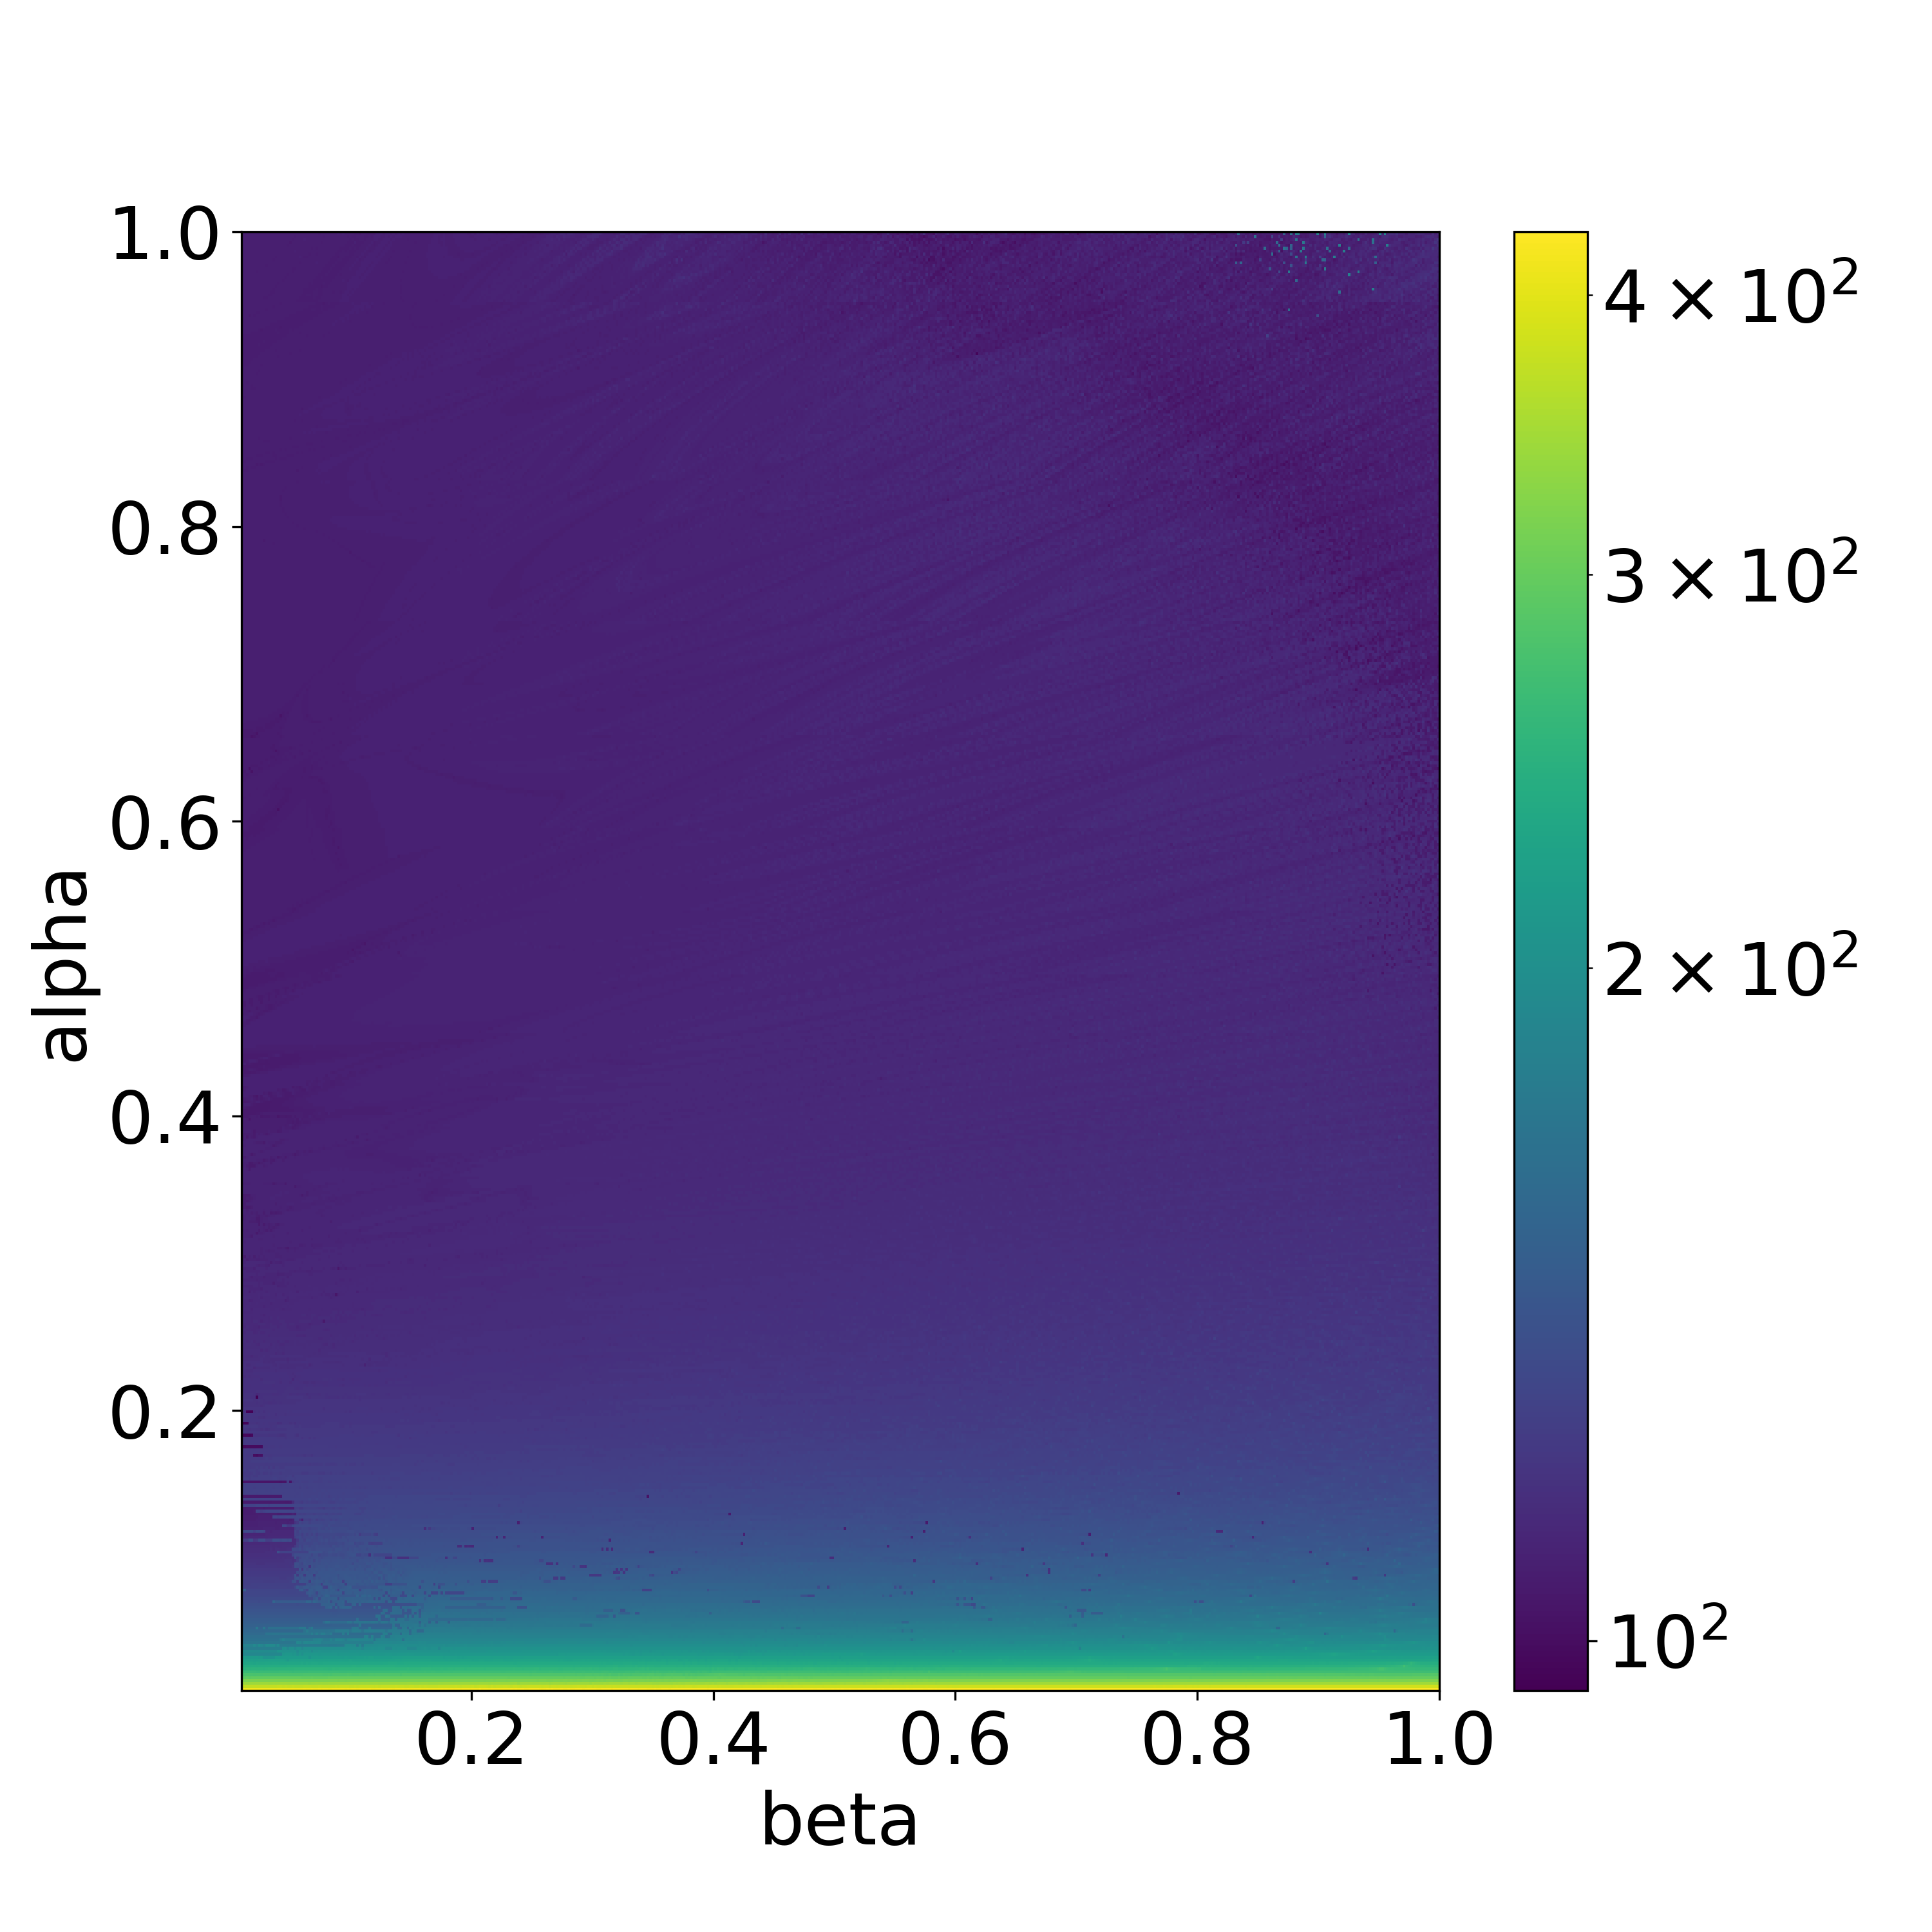
\includegraphics[width=1\textwidth]{images/analysis_RKF45_TS.png}
       	\subcaption{Number of required timesteps} 
        \label{fig:numberTimeStepsRKF45}
    \end{subfigure}
    \begin{subfigure}{0.32\textwidth}
    	\centering
    	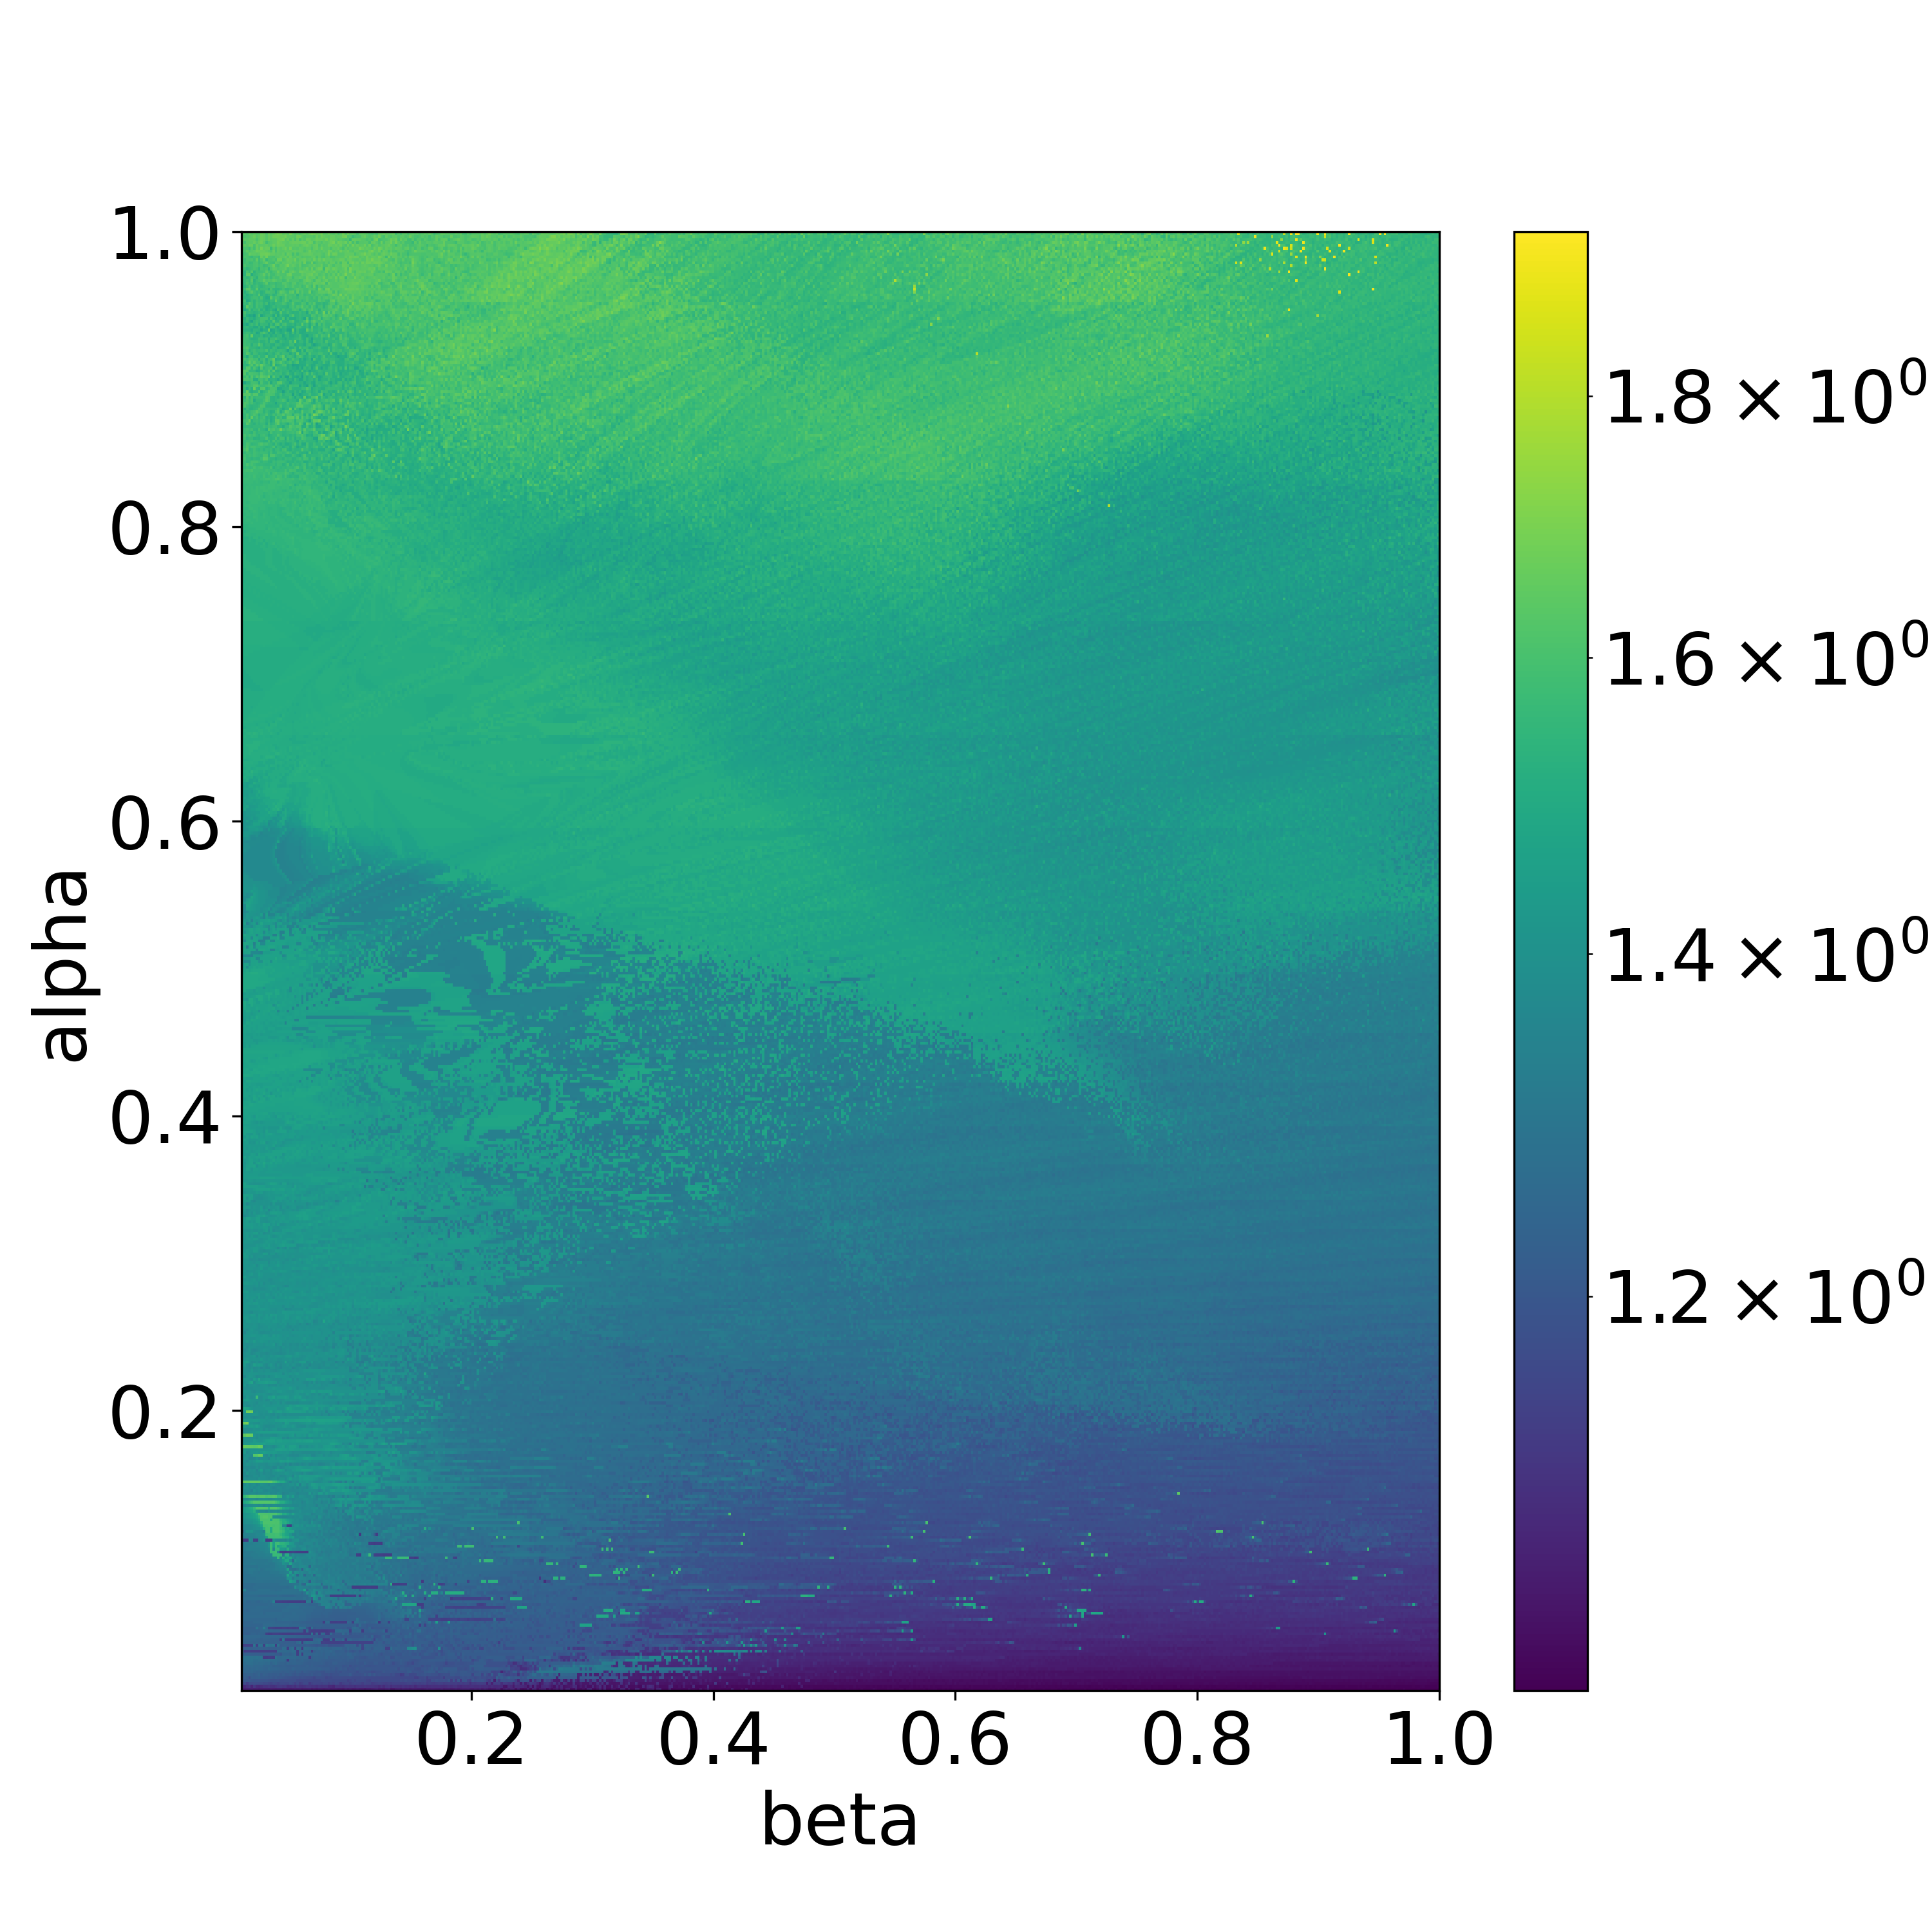
\includegraphics[width=1\textwidth]{images/analysis_RKF45_NI.png}
       	\subcaption{Average number of iterations per timestep} 
        \label{fig:numberIterationTSRKF45}
    \end{subfigure}
    \begin{subfigure}{0.32\textwidth}
    	\centering
    	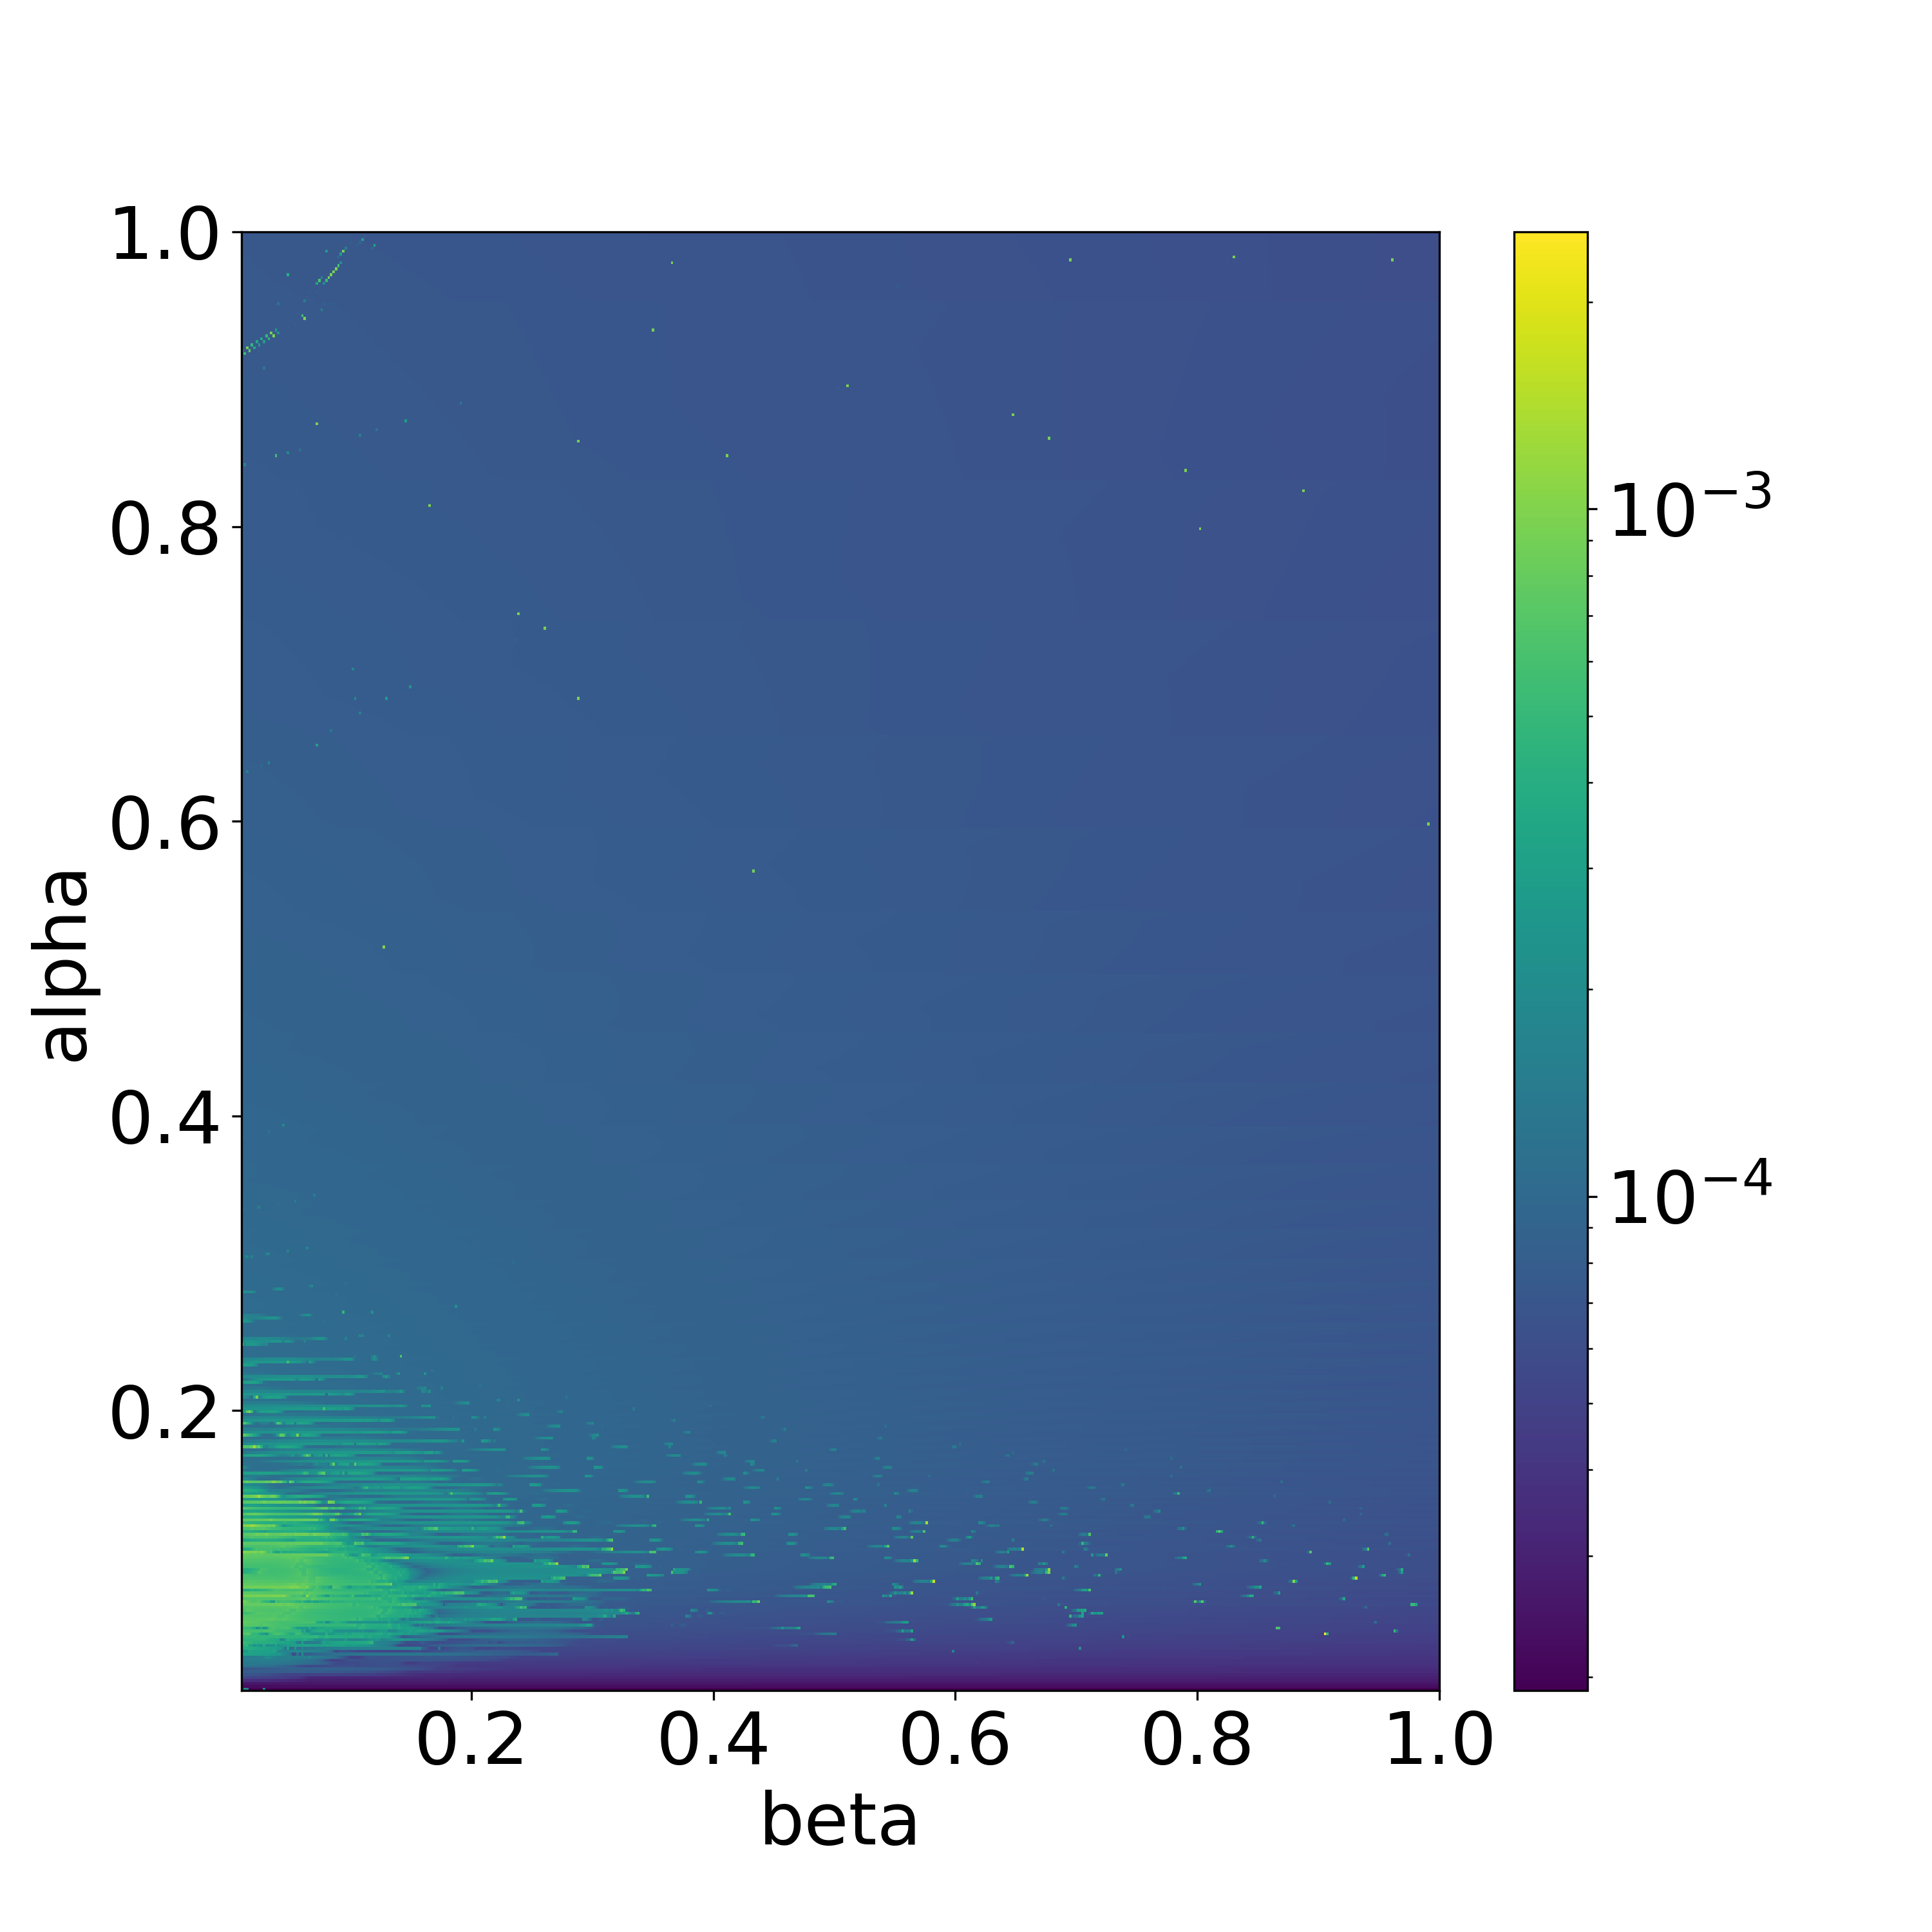
\includegraphics[width=1\textwidth]{images/analysis_RKF45_psi.png}
       	\subcaption{Absolute error of the variable $\psi$} 
        \label{fig:numberNumericalSchemeRKF45}
    \end{subfigure}
    \caption{Impact of the parameters $\alpha$ and $\beta$ of the PI controller on the number of required iterations to solve the model problem from \autoref{eq:first_DAE_ODE} using the explicit Runge-Kutta-Fehlberg method (\textbf{RKF45}) for a simulation time of $t=5.0s$}
    \label{fig:ParametersPIControllerRKF45}
\end{figure}


\begin{figure}[H]
    \centering
    \begin{subfigure}{0.32\textwidth}
    	\centering
    	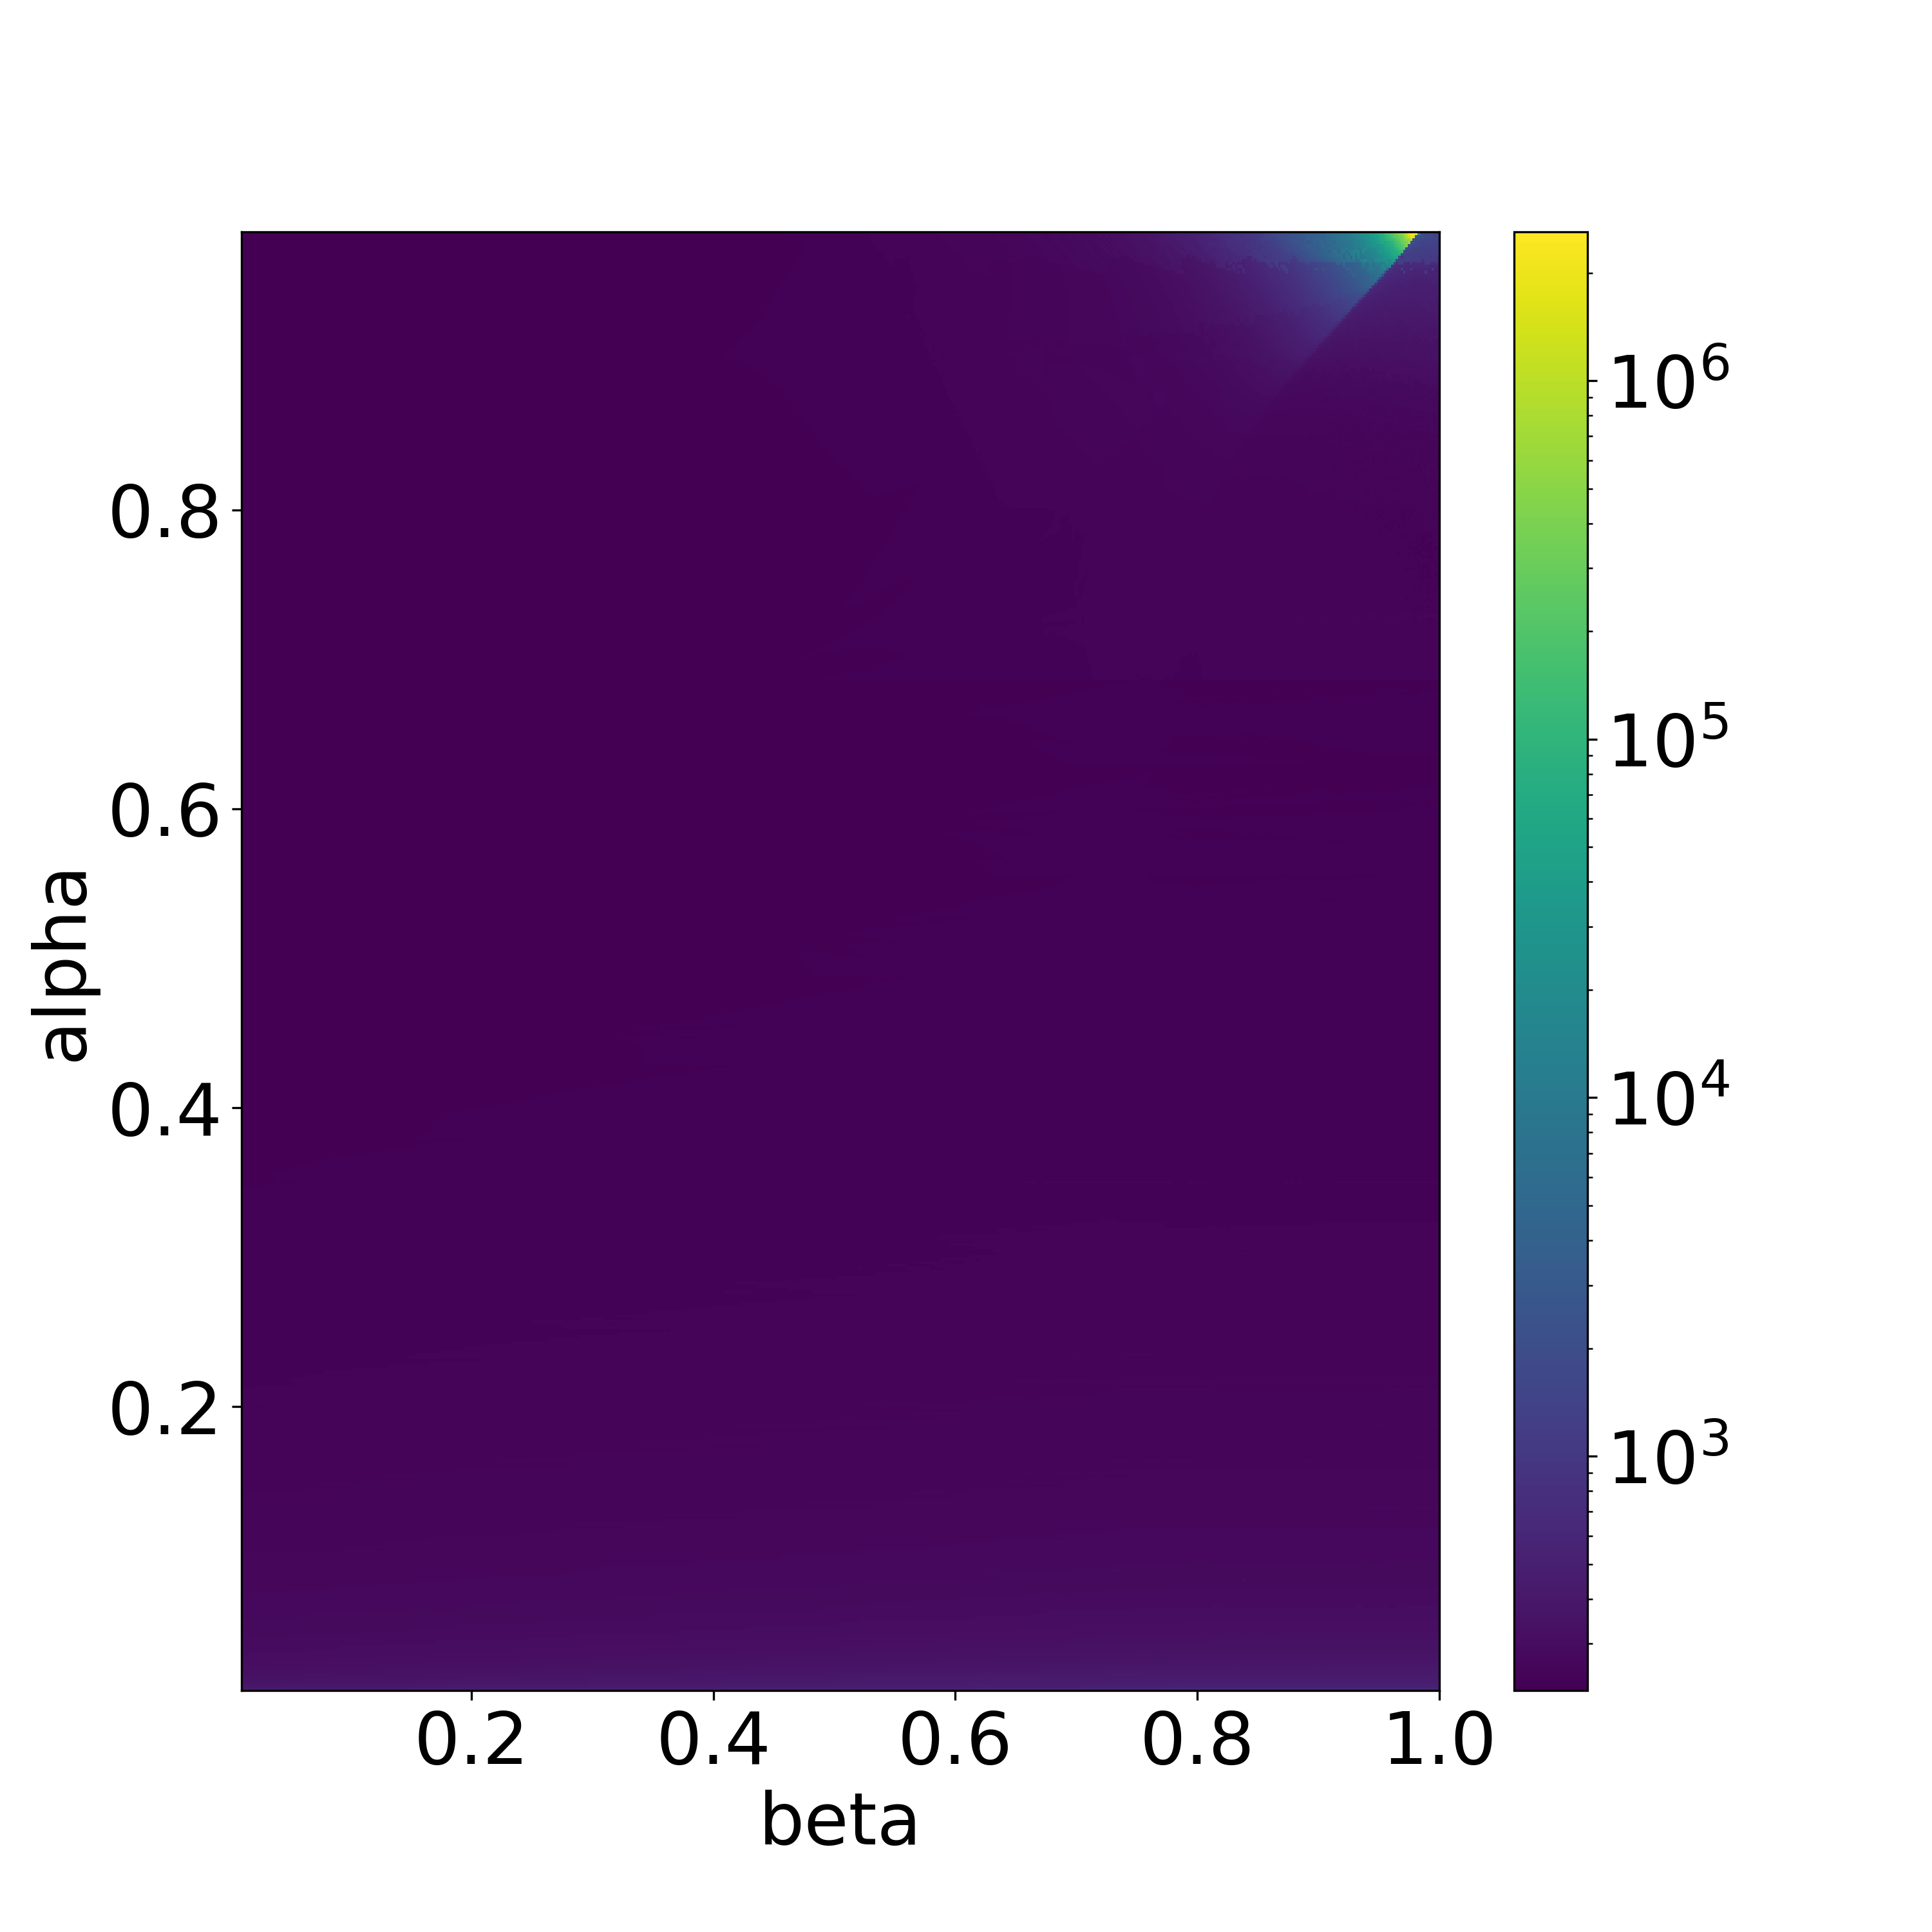
\includegraphics[width=1\textwidth]{images/analysis_BDF12_TS.png}
       	\subcaption{Number of required timesteps} 
        \label{fig:numberTimeStepsBDF12}
    \end{subfigure}
    \begin{subfigure}{0.32\textwidth}
    	\centering
    	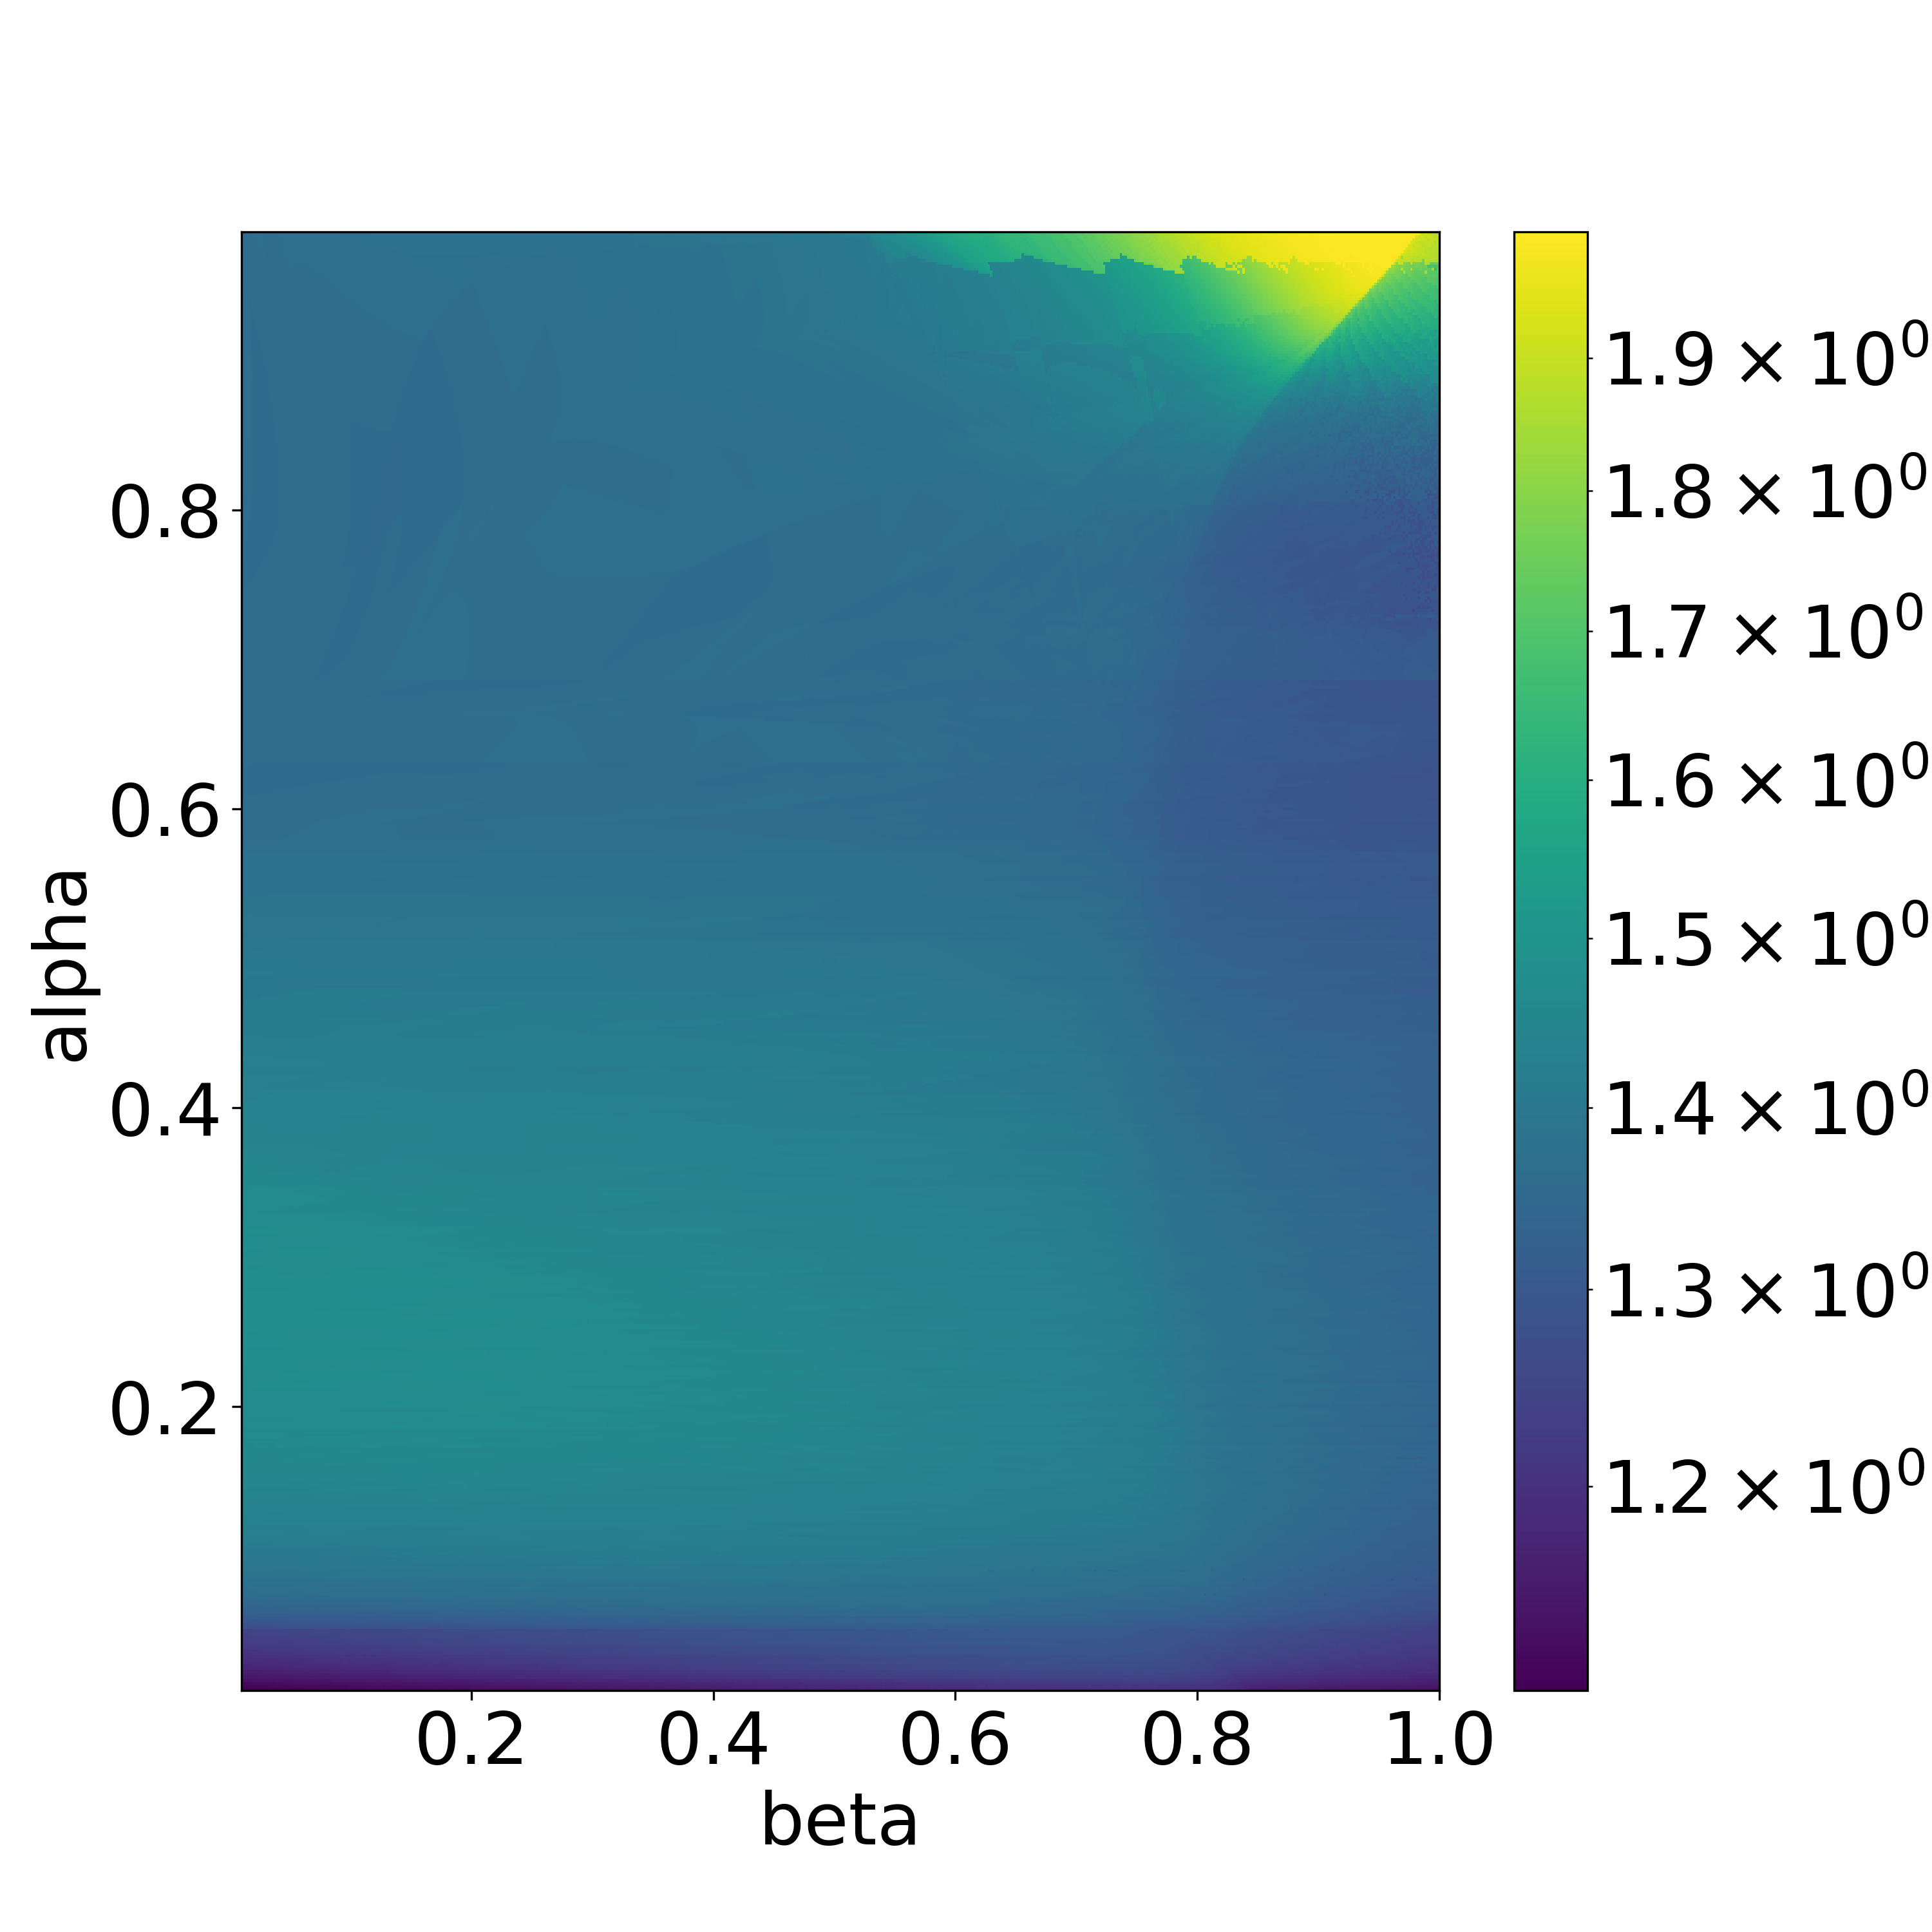
\includegraphics[width=1\textwidth]{images/analysis_BDF12_NI.png}
       	\subcaption{Average number of iterations per timestep} 
        \label{fig:numberIterationTSBDF12}
    \end{subfigure}
    \begin{subfigure}{0.32\textwidth}
    	\centering
    	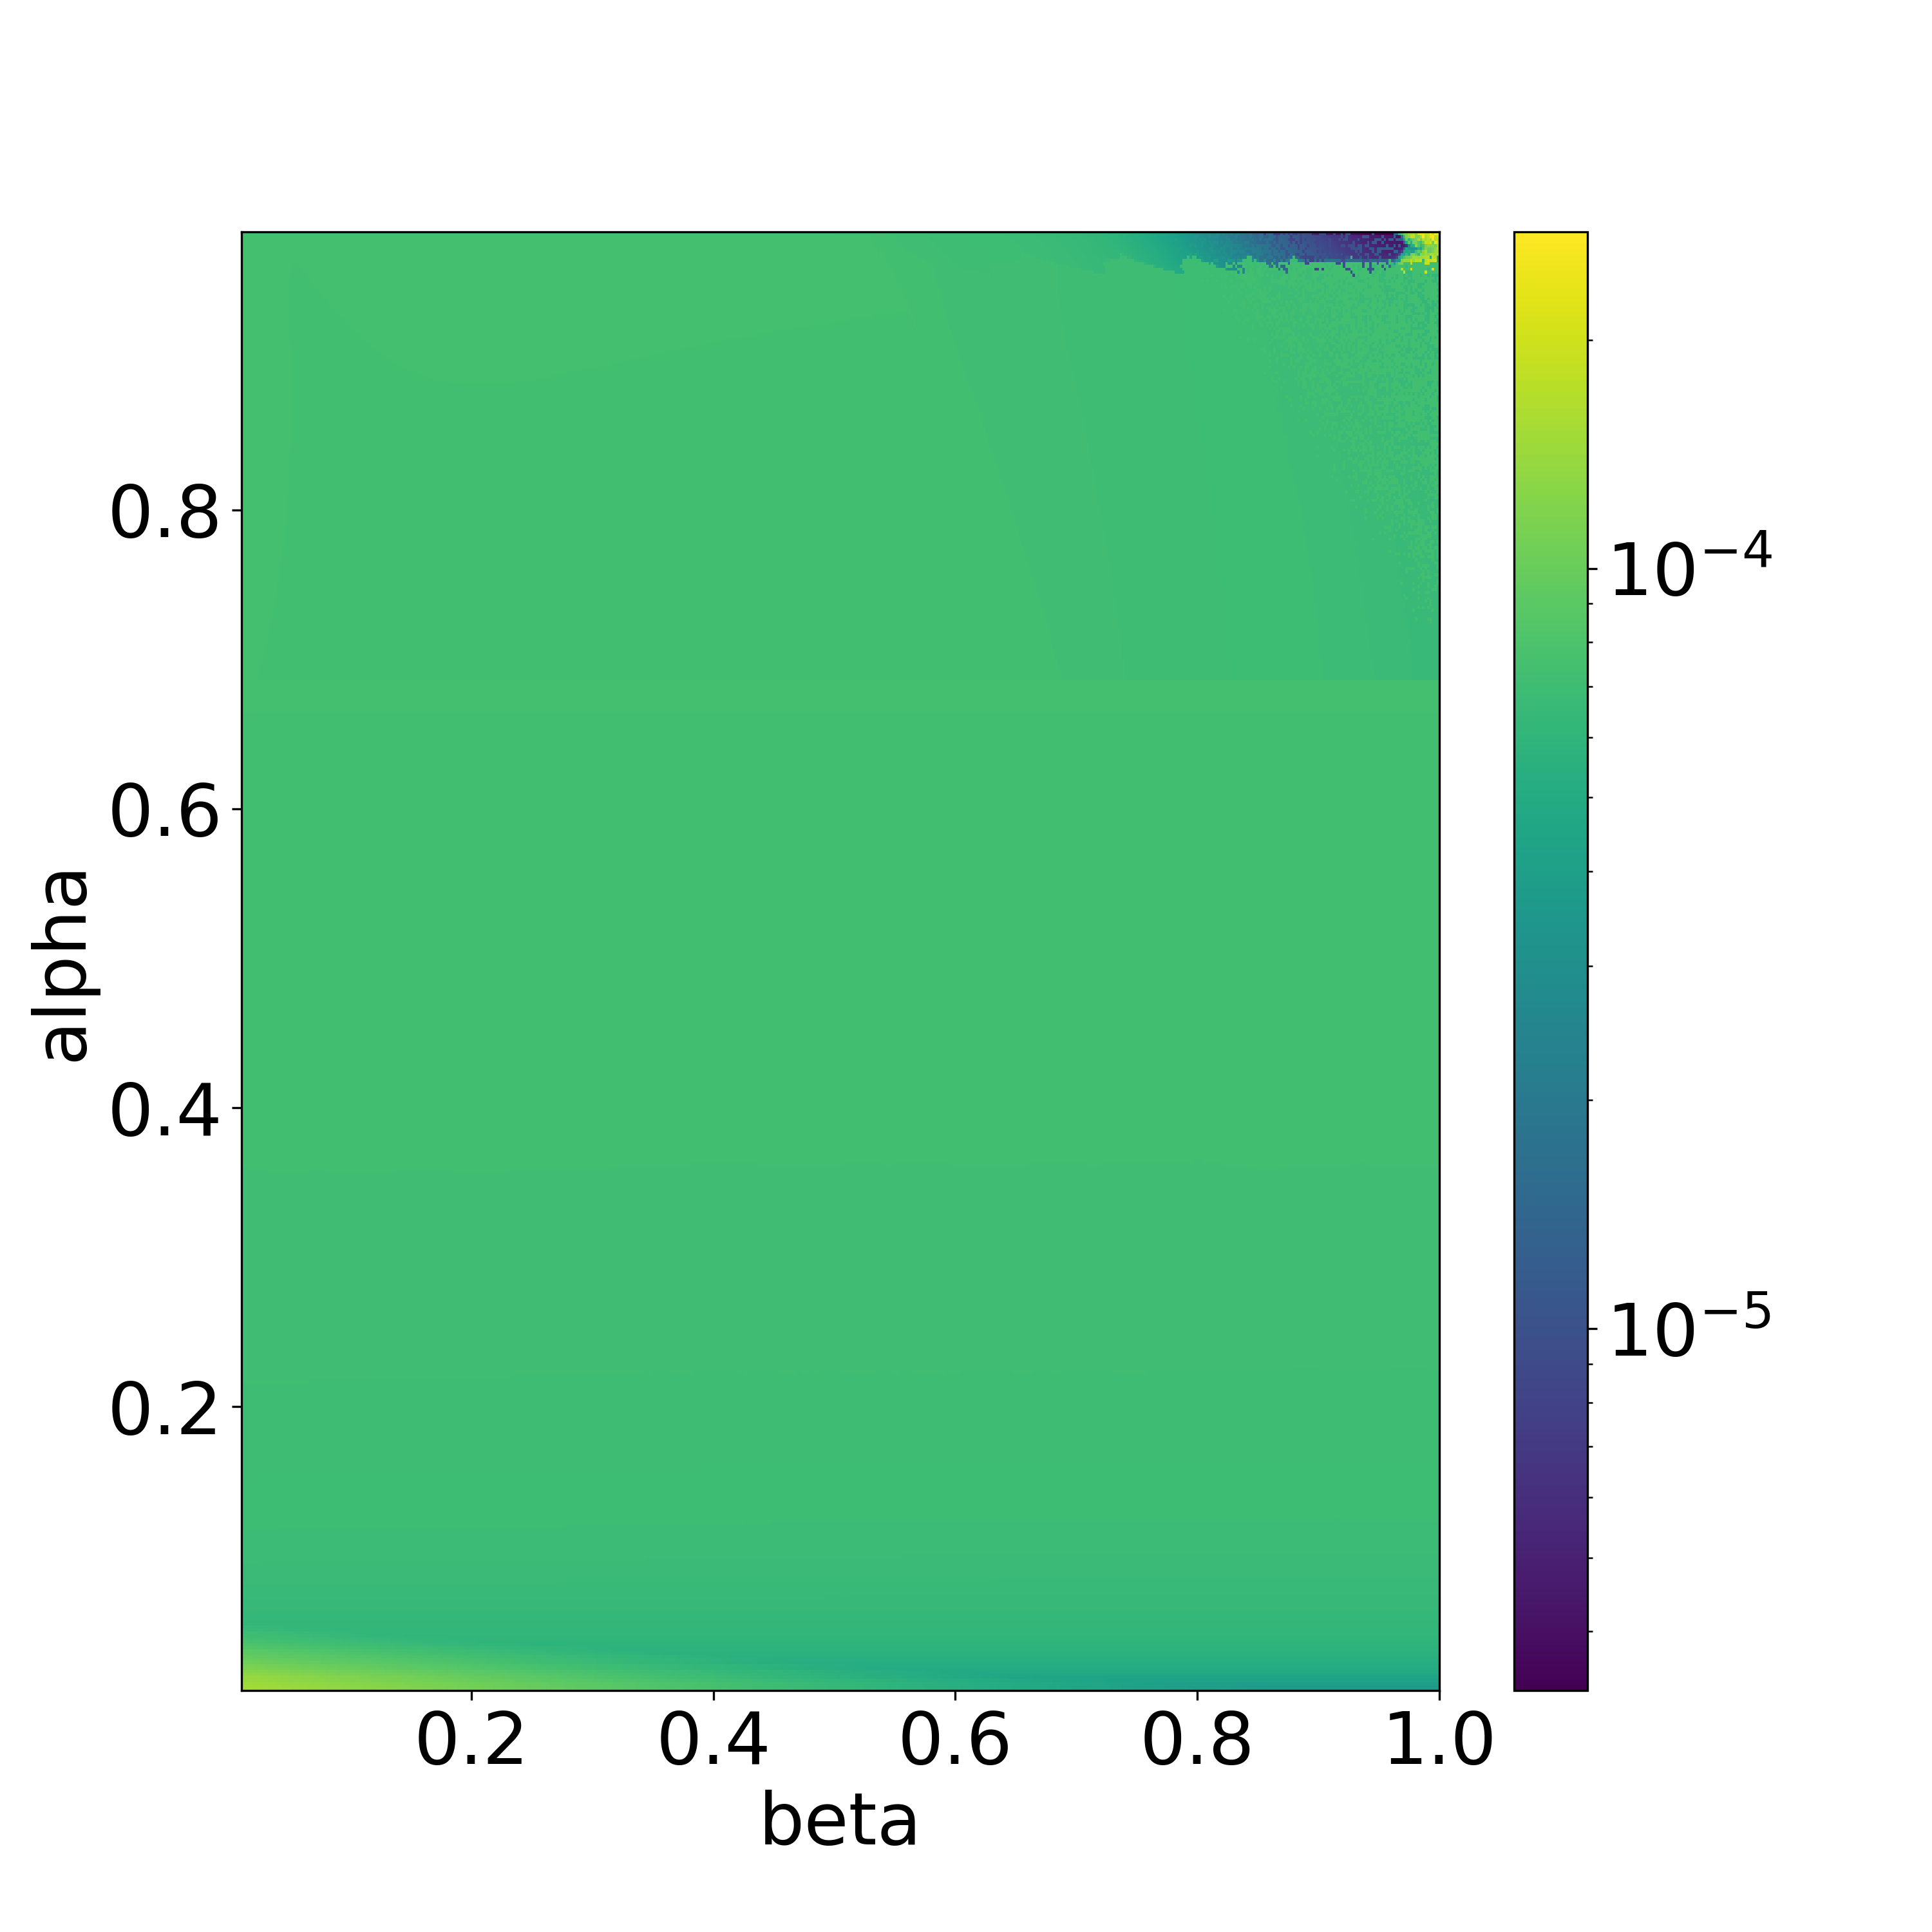
\includegraphics[width=1\textwidth]{images/analysis_BDF12_psi.png}
       	\subcaption{Absolute error of the variable $\psi$} 
        \label{fig:numberNumericalSchemeBDF12}
    \end{subfigure}
    \caption{Impact of the parameters $\alpha$ and $\beta$ of the PI controller on the number of required iterations to solve the model problem from \autoref{eq:first_DAE_ODE} using the implicit BDF method of first order (\textbf{BDF12}) for a simulation time of $t=5.0s$}
    \label{fig:ParametersPIControllerBDF12}
\end{figure}


\begin{figure}[H]
    \centering
    \begin{subfigure}{0.32\textwidth}
    	\centering
    	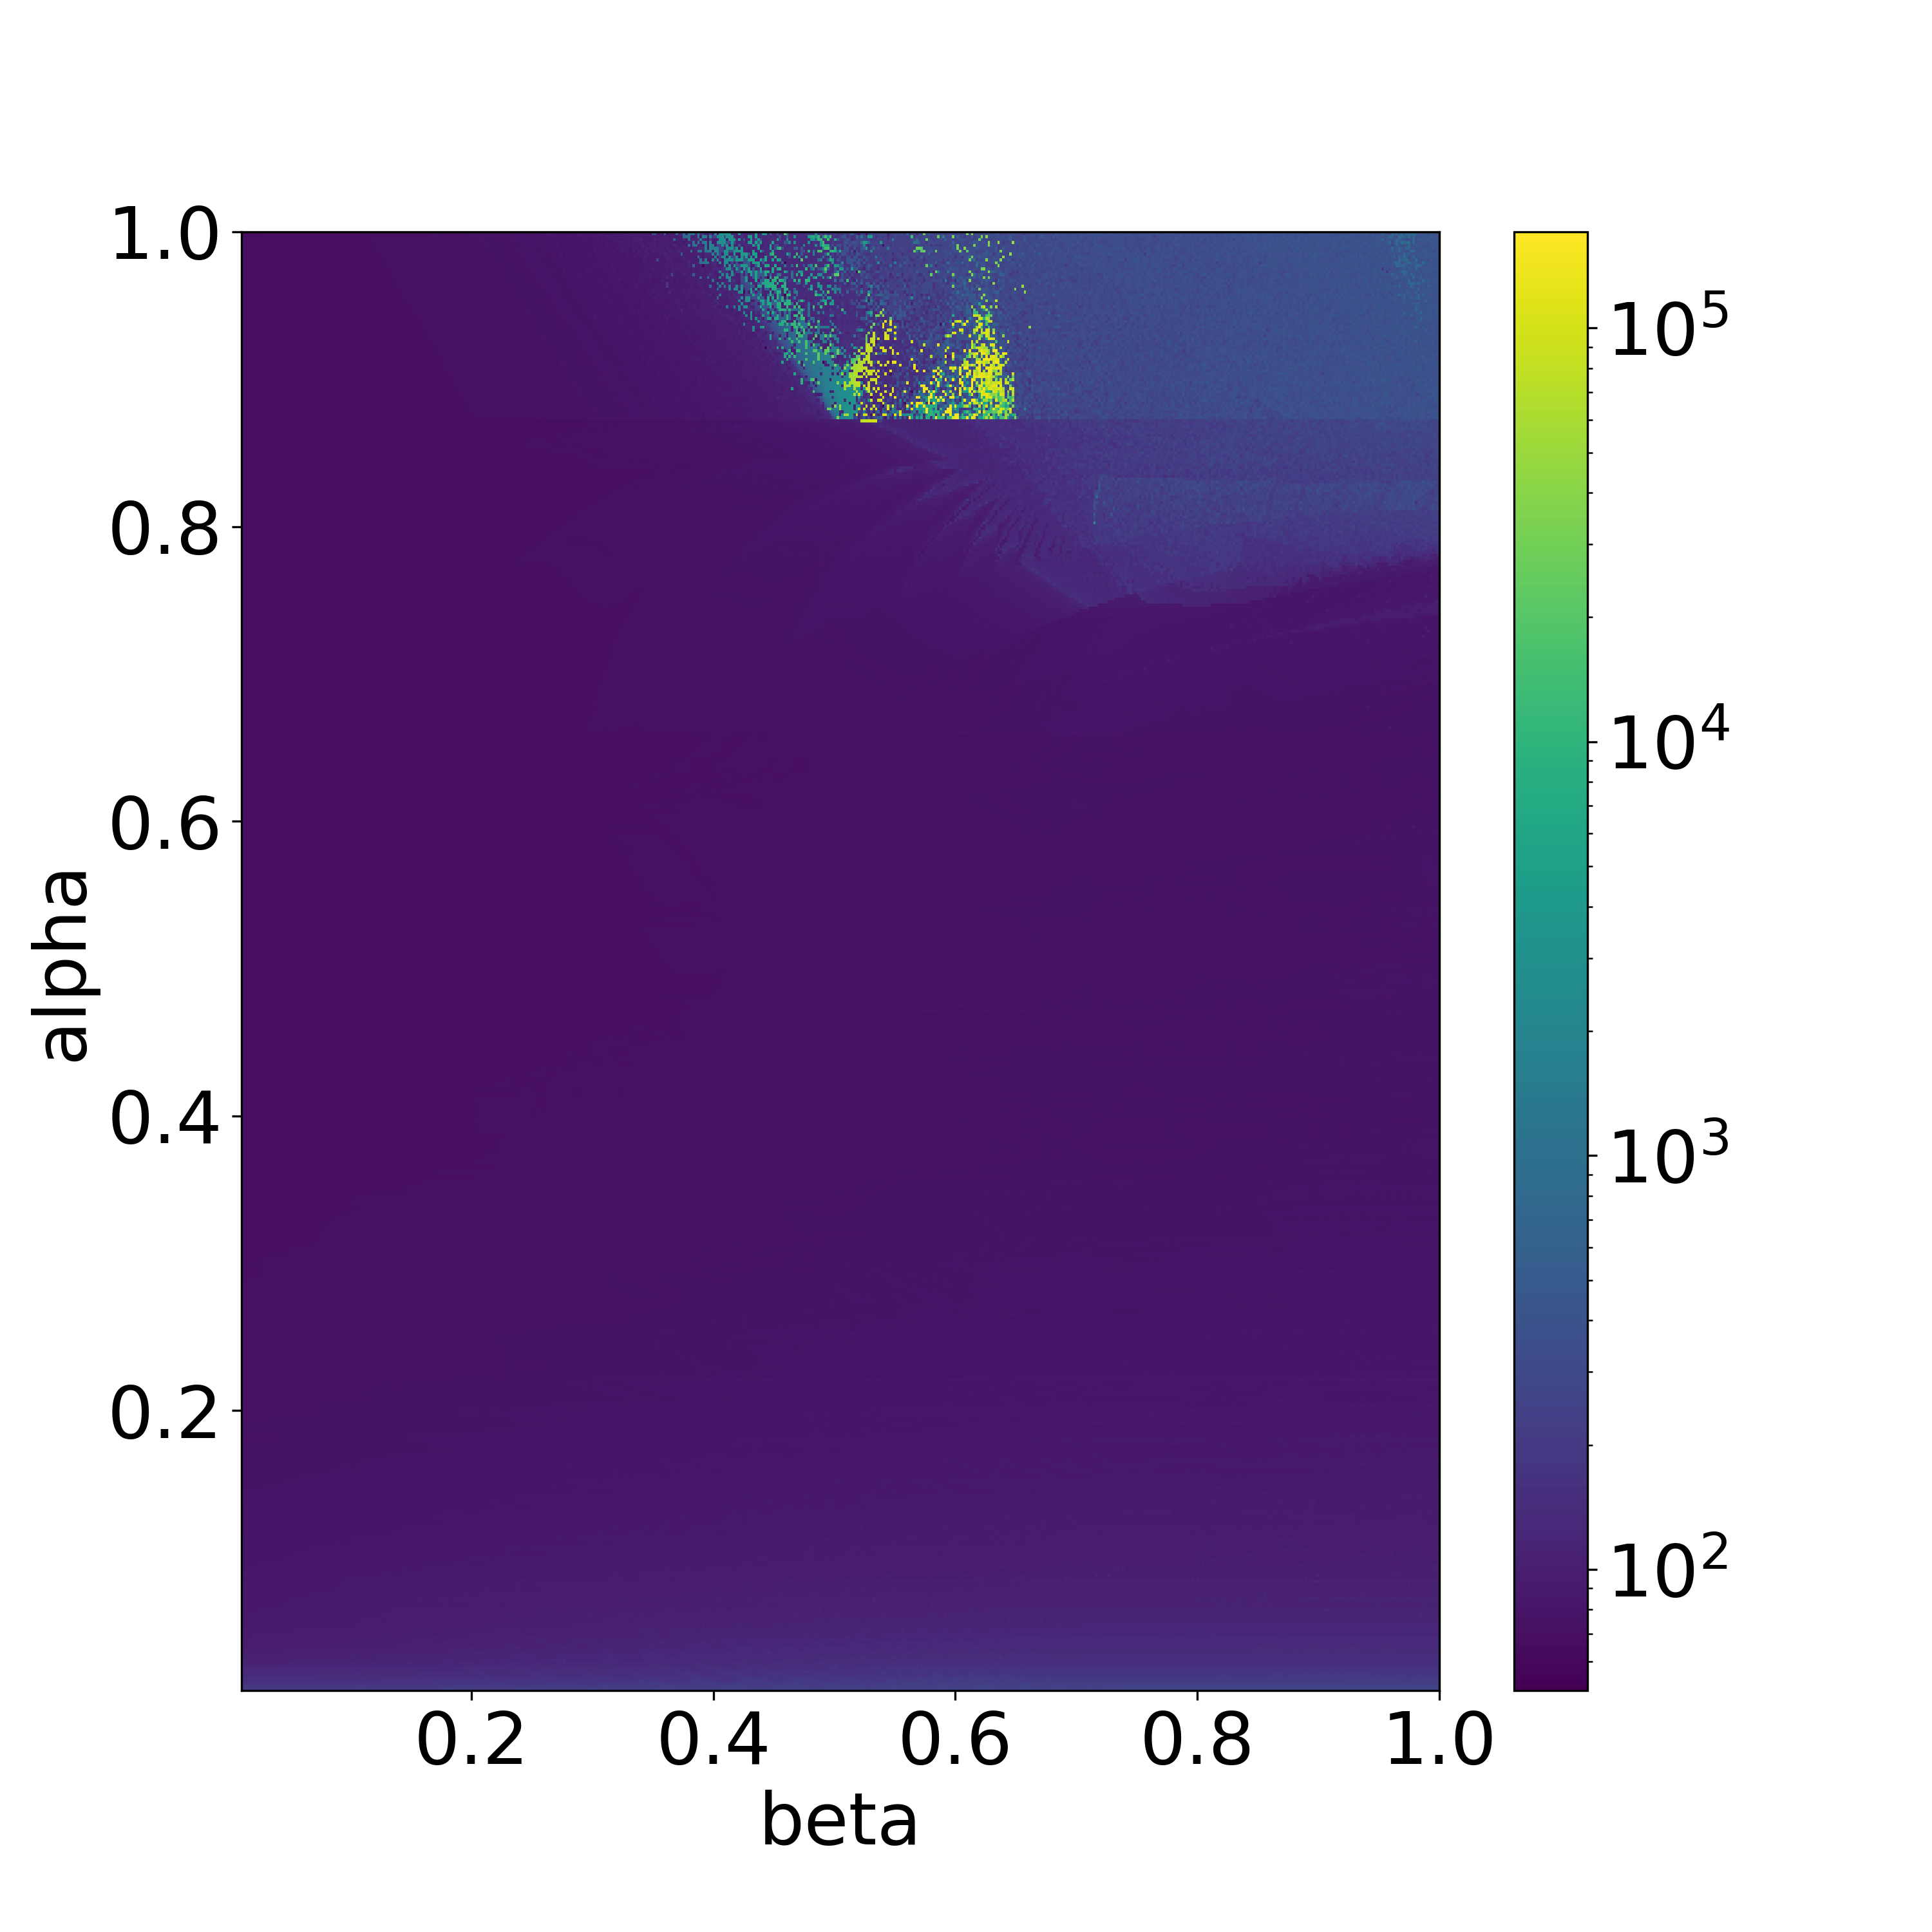
\includegraphics[width=1\textwidth]{images/analysis_BDF23_TS.png}
       	\subcaption{Number of required timesteps} 
        \label{fig:numberTimeStepsBDF23}
    \end{subfigure}
    \begin{subfigure}{0.32\textwidth}
    	\centering
    	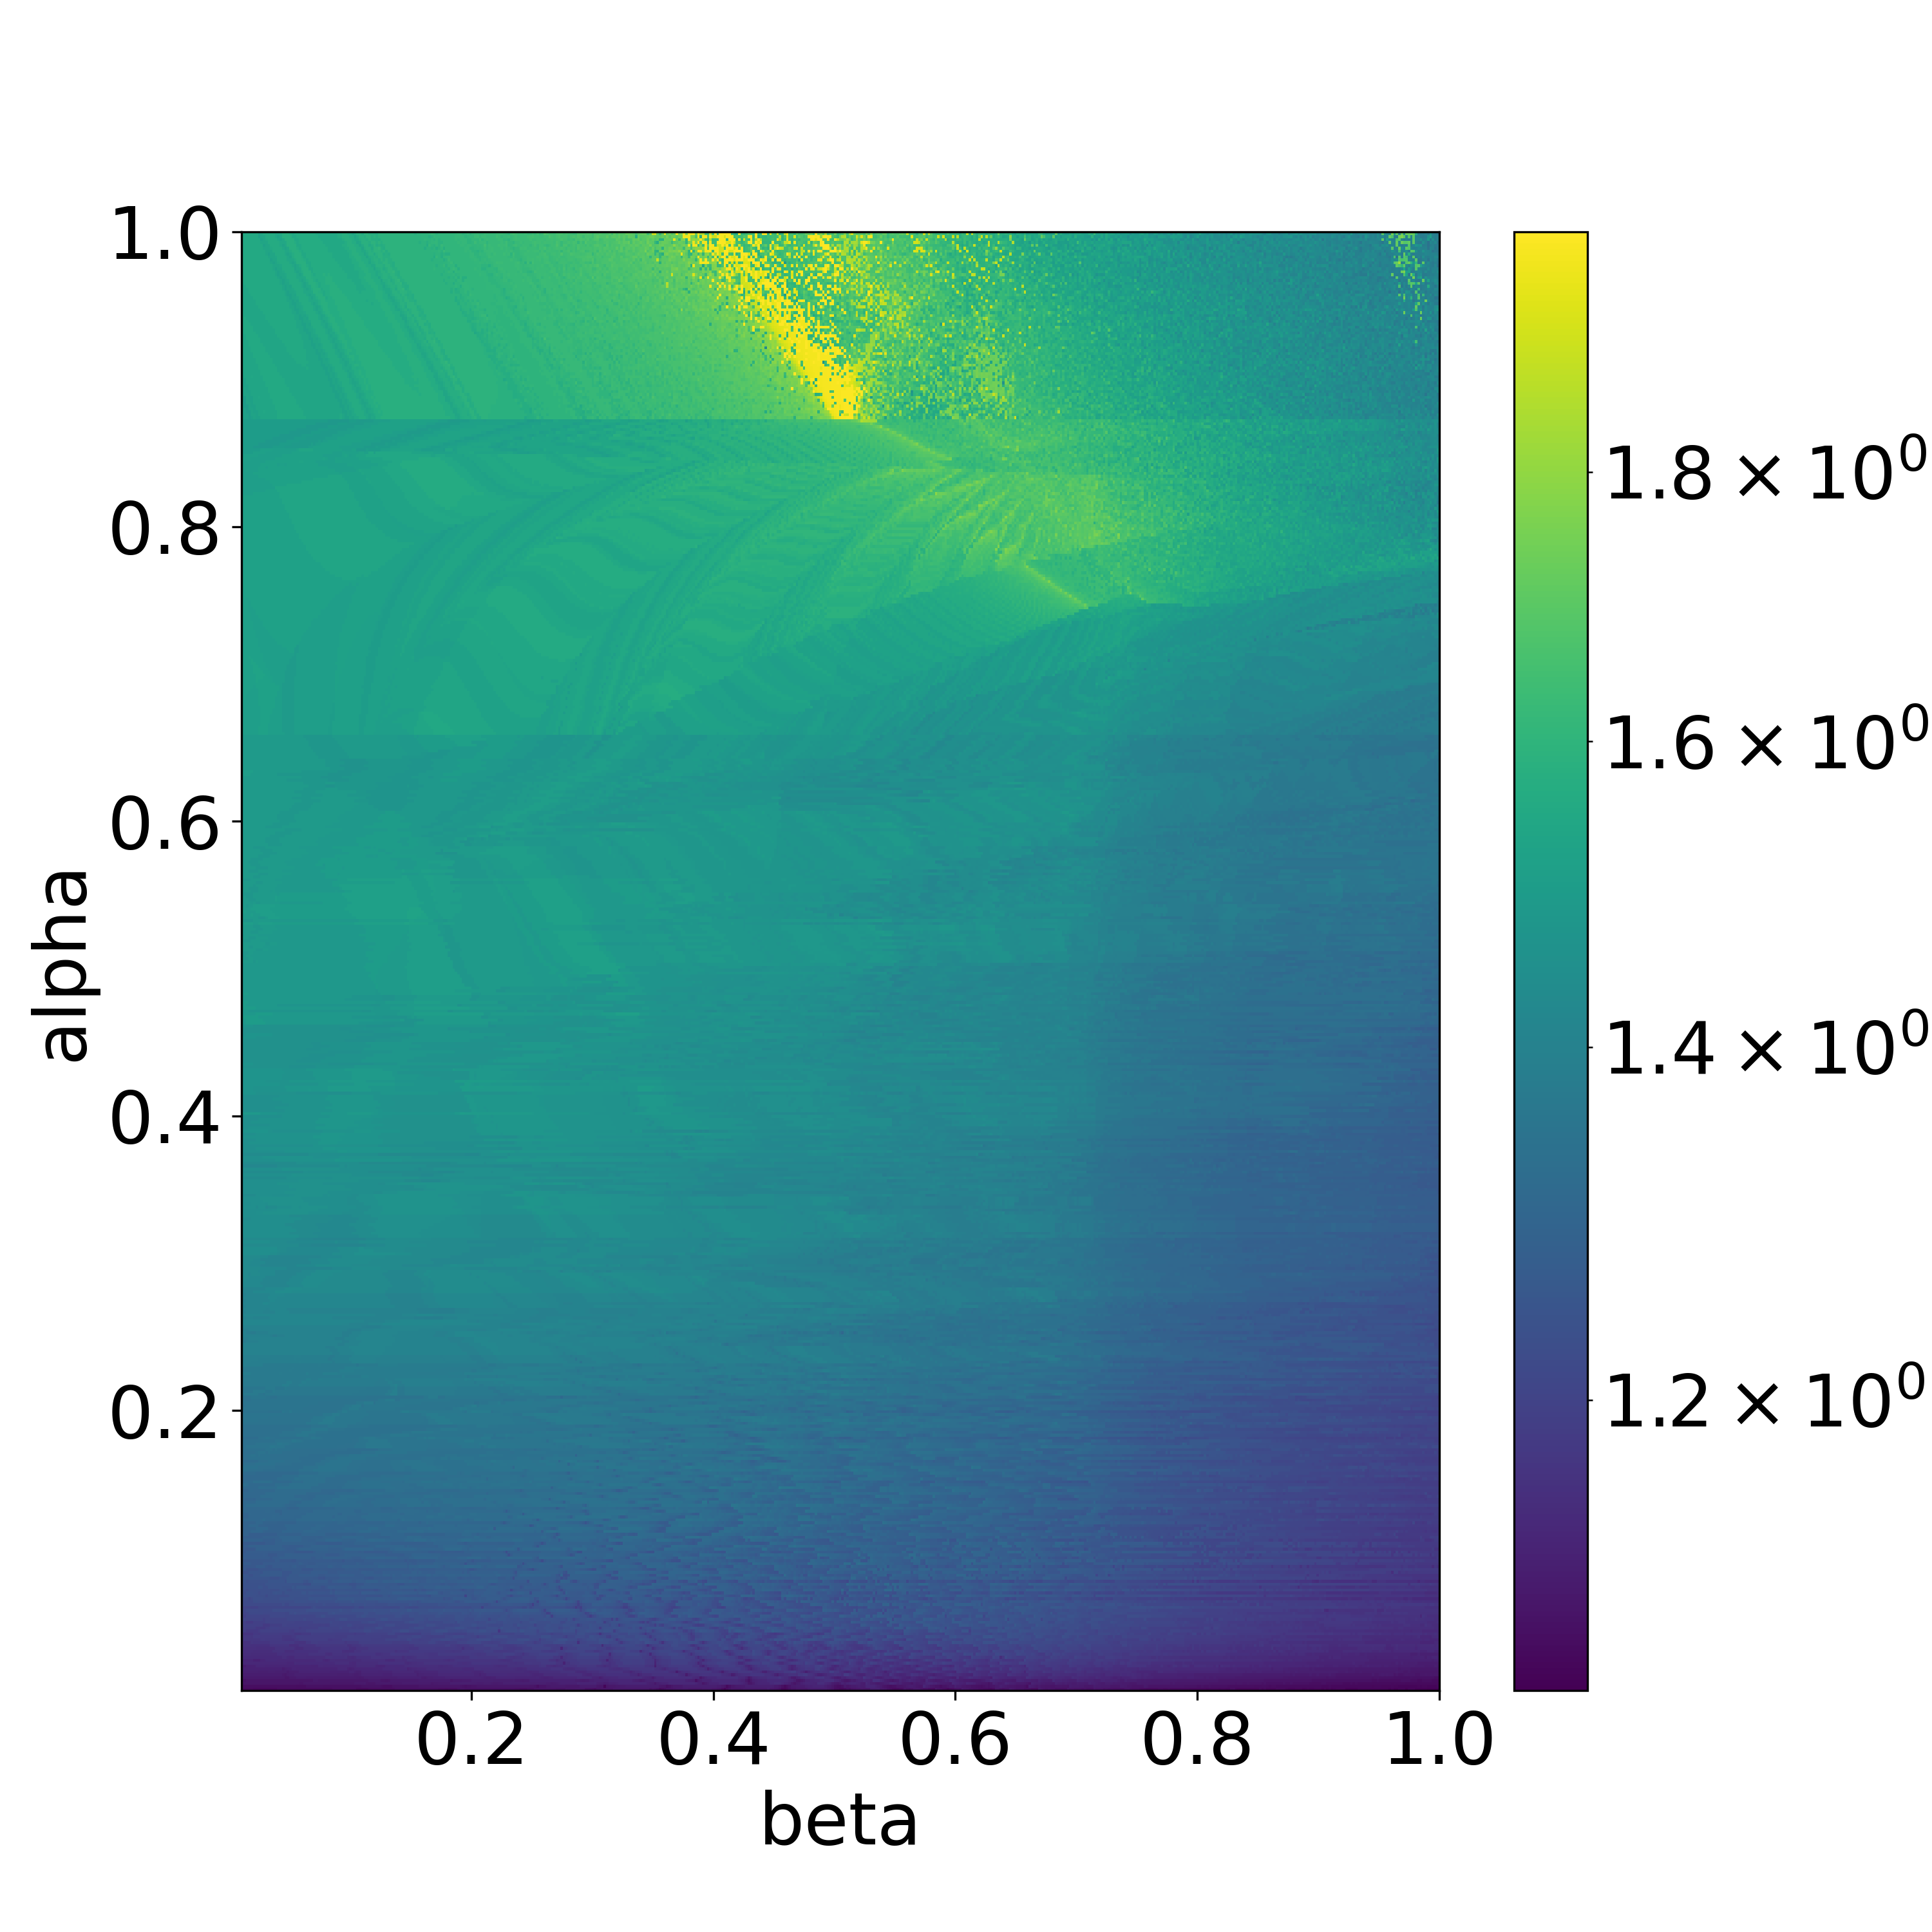
\includegraphics[width=1\textwidth]{images/analysis_BDF23_NI.png}
       	\subcaption{Average number of iterations per timestep} 
        \label{fig:numberIterationTSBDF23}
    \end{subfigure}
    \begin{subfigure}{0.32\textwidth}
    	\centering
    	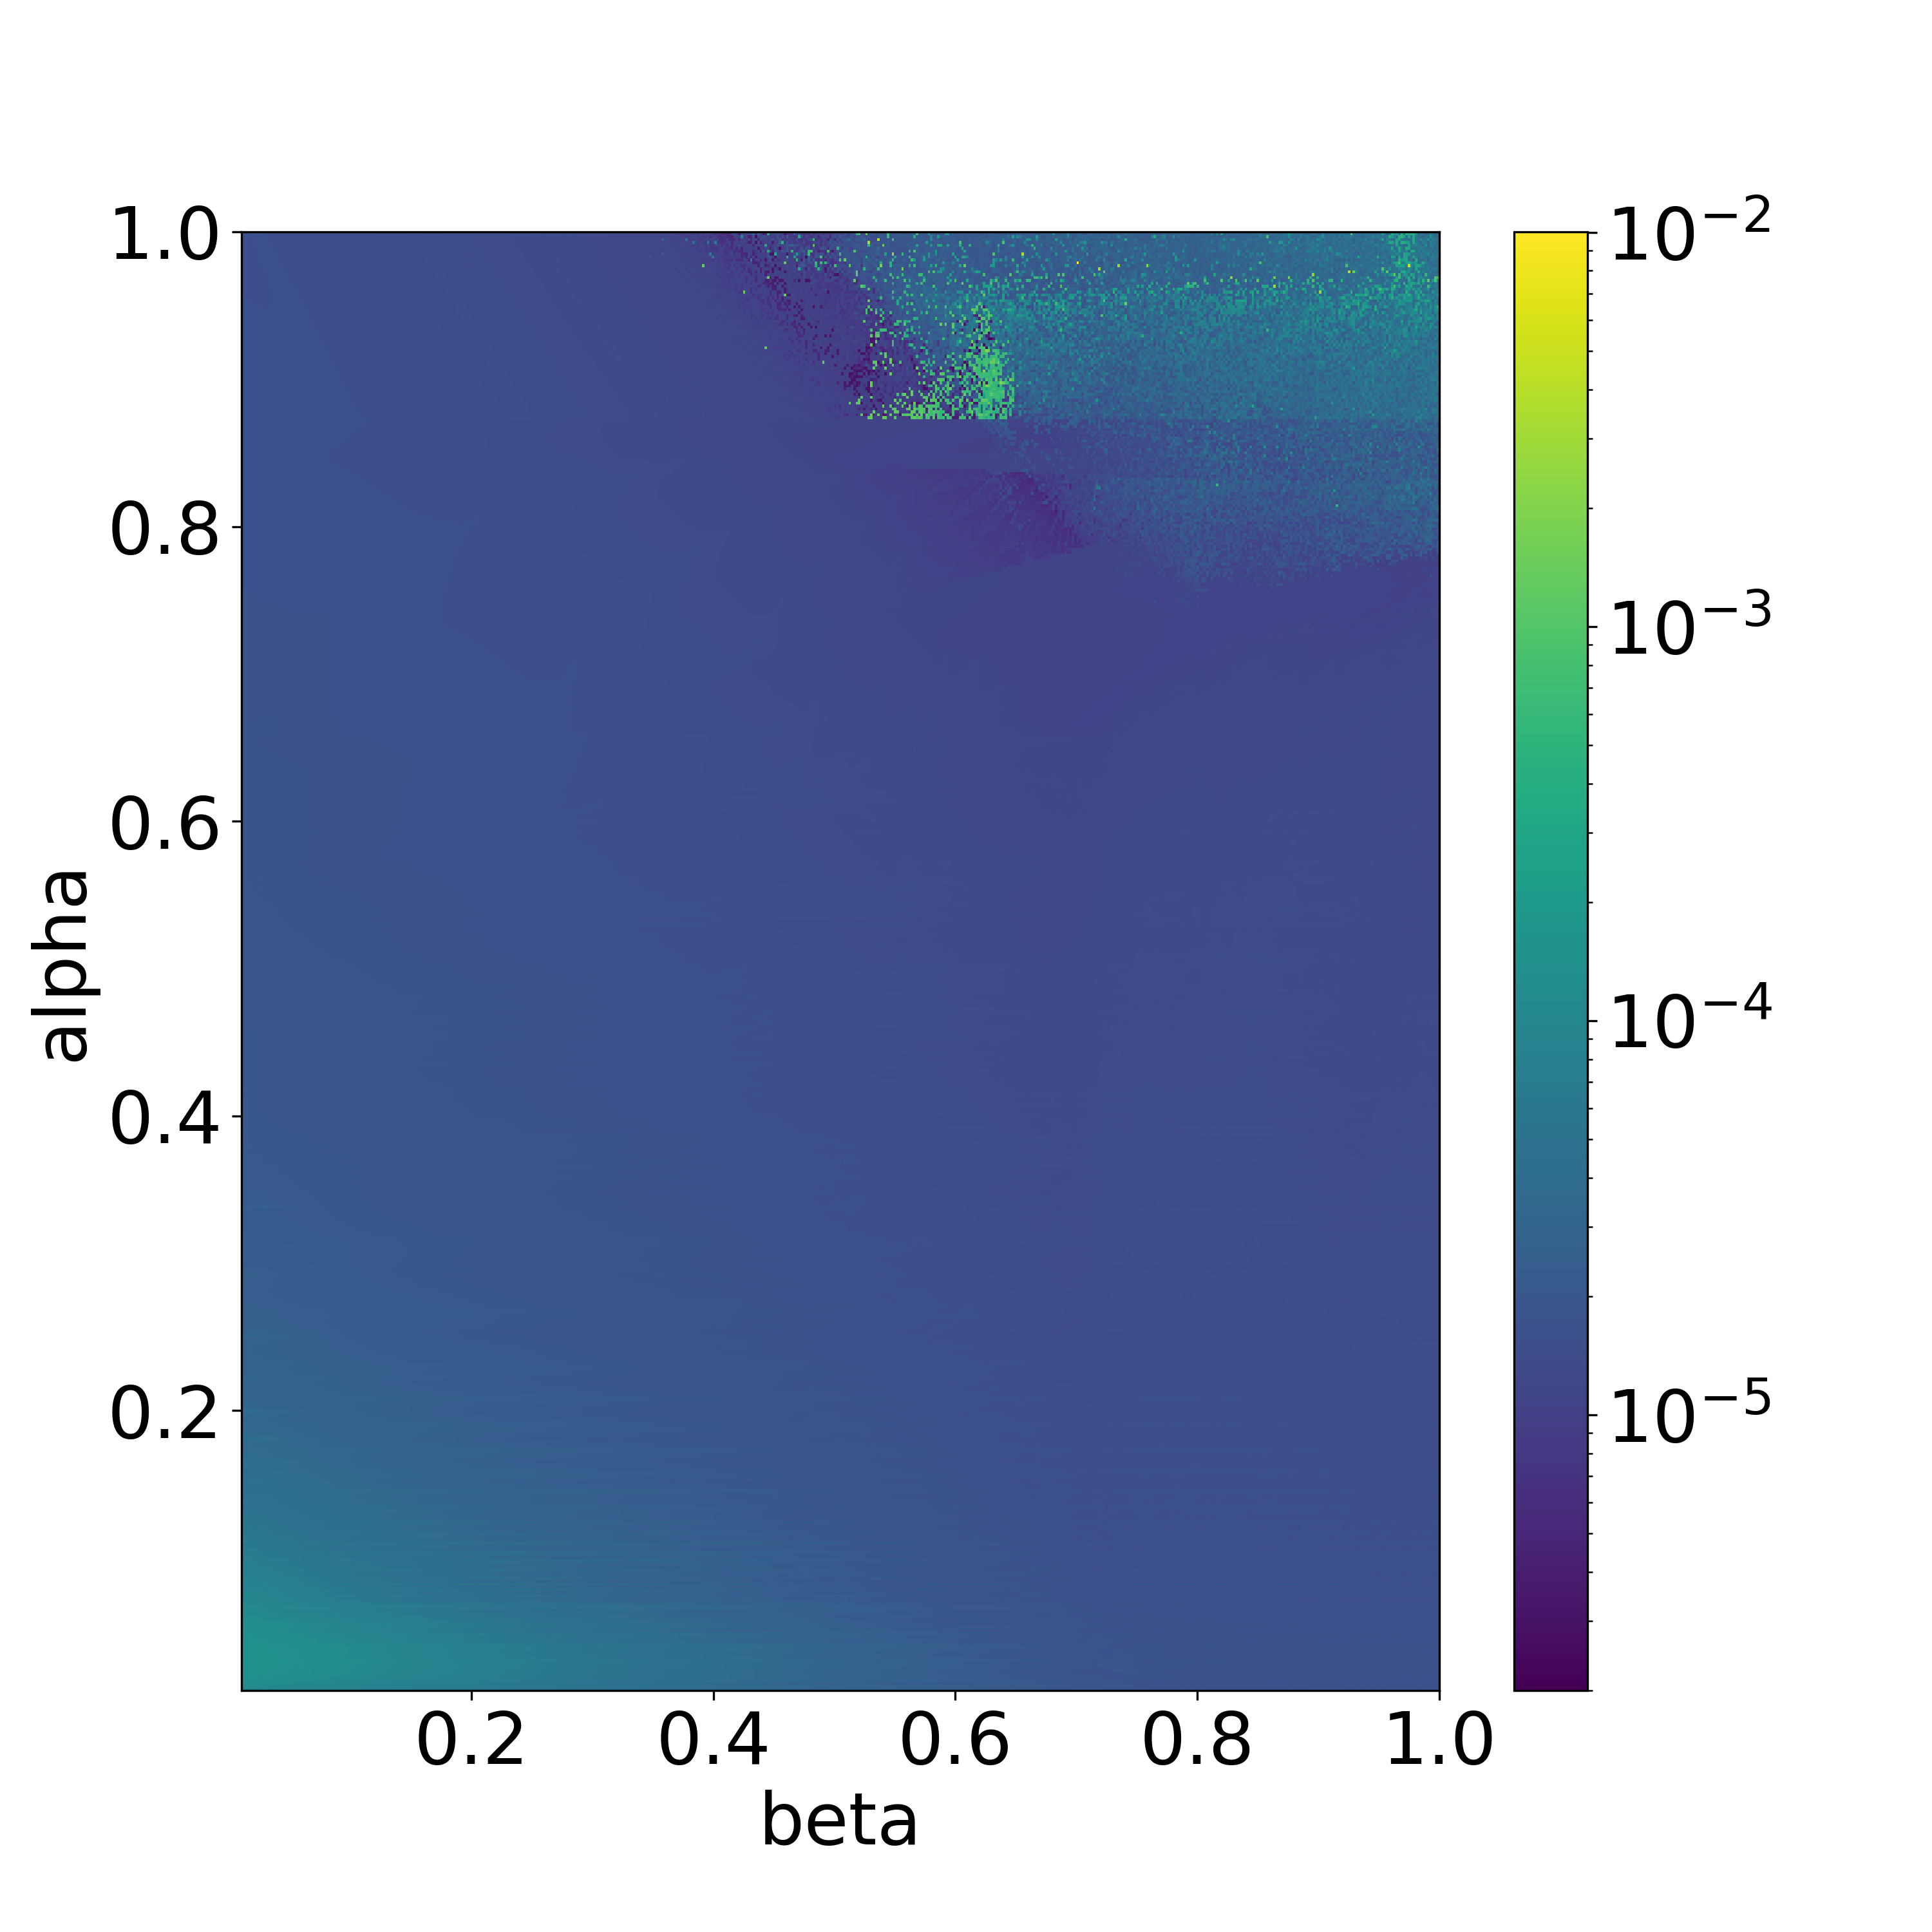
\includegraphics[width=1\textwidth]{images/analysis_BDF23_psi.png}
       	\subcaption{Absolute error of the variable $\psi$} 
        \label{fig:numberNumericalSchemeBDF23}
    \end{subfigure}
    \caption{Impact of the parameters $\alpha$ and $\beta$ of the PI controller on the number of required iterations to solve the model problem from \autoref{eq:first_DAE_ODE} using the implicit BDF method of second order (\textbf{BDF23}) for a simulation time of $t=5.0s$}
    \label{fig:ParametersPIControllerBDF23}
\end{figure}

We chose as parameters: 
\begin{itemize}
    \item for \textbf{RKF45}: $\alpha=0.4$ and $\beta=0.6$
    \item for \textbf{BDF12}: $\alpha=0.9$ and $\beta=0.4$
    \item for \textbf{BDF23}: $\alpha=0.9$ and $\beta=0.4$
\end{itemize}

---Put some more explanations here --- \\
---Find the balance between number of iterations and accuracy --- \\
---Numerical instabilities for the implicit methods for high values of $\alpha$ and $\beta$ --- \\
failure of the error estimate? too small timesteps? \\ 

\section{Comparison of the Numerical Schemes}
So far, one explicit (RKF45) and two implicit (BDF12, BDF23) numerical solvers have been implemented for the initial DAE in \autoref{eq:first_DAE_algeb} and their ideal parameter choice for their use with a PI controller has been discussed. Now, the quality of the solutions is compared. \\

\subsection{Numerical solutions}
Again, the allowed tolerance of the PI controller is set to $\epsilon=1\cdot 10^{-6}$. The method of the manufactured solutions is chosen to have an analytical solution against which numerical computations can be compared. The parameters $t_e$ and $t_w$ are chosen in a way that the velocity is initially close to zero and increases to 1 over the time span of one second at the middle of the simulation time. \autoref{fig:timeEvolutionValues} depicts the solution variables $\psi$ and $V$ over time for all three solvers. The expected form of the $\text{atan}$ function centered around $2.5$ for the velocity is obtained with all methods and the results for $\psi$ match too, as $\psi$ decreases linearly before it stabilizes around zero as the velocity increases. \\
If adaptive timestepping methods are used, the actual size of the timestep $h_n$ is of particular interest. Since at each timestep, the right-hand side of the ODE and the algebraic equation have to be solved a fixed number of times, a method that allows larger timesteps is considered more efficient. As shown in \autoref{fig:timeEvolutionDT}, this metric varies greatly with the chosen numerical solver. The simulation time can be roughly split into three sections: The first phase corresponds to low velocity and decreasing $\psi$ until the time $t=2.0s$. In it, the RKF45 and BDF23 methods allow for rather similarly large timestep sizes, whereas the BDF12 method is restricted to timestep sizes which are about fives times smaller. The second phase is marked by the fast increase in velocity and the stabilization of $\psi$. Such rapid changes in the solution should imply shorter timesteps to obtain accurate solutions, especially for RKF45, because explicit schemes face stability issues for stiff problems. Indeed, a decrease in the timestep size can be observed for all three methods, however the explicit RKF45 performs much better than expected with timesteps that are about twice as long as using BDF23. As previously, BDF12 has the worst performance of all three methods which much smaller timesteps. In the last phase, when the velocity approaches 1 and $\psi$ remains close to 0, the two implicit BDF methods reach very large timesteps with an increasing trend, whereas the the timesteps generated by the controller RKF45 stagnate at a rather low value. Overall, BDF23 performs best with 69 timesteps, followed by RKF45 with 120 and finally BDF12 needs 230 timesteps to execute the whole simulation. 

\begin{figure}[H]
    \centering
    \begin{subfigure}{0.43\textwidth}
    	\centering
    	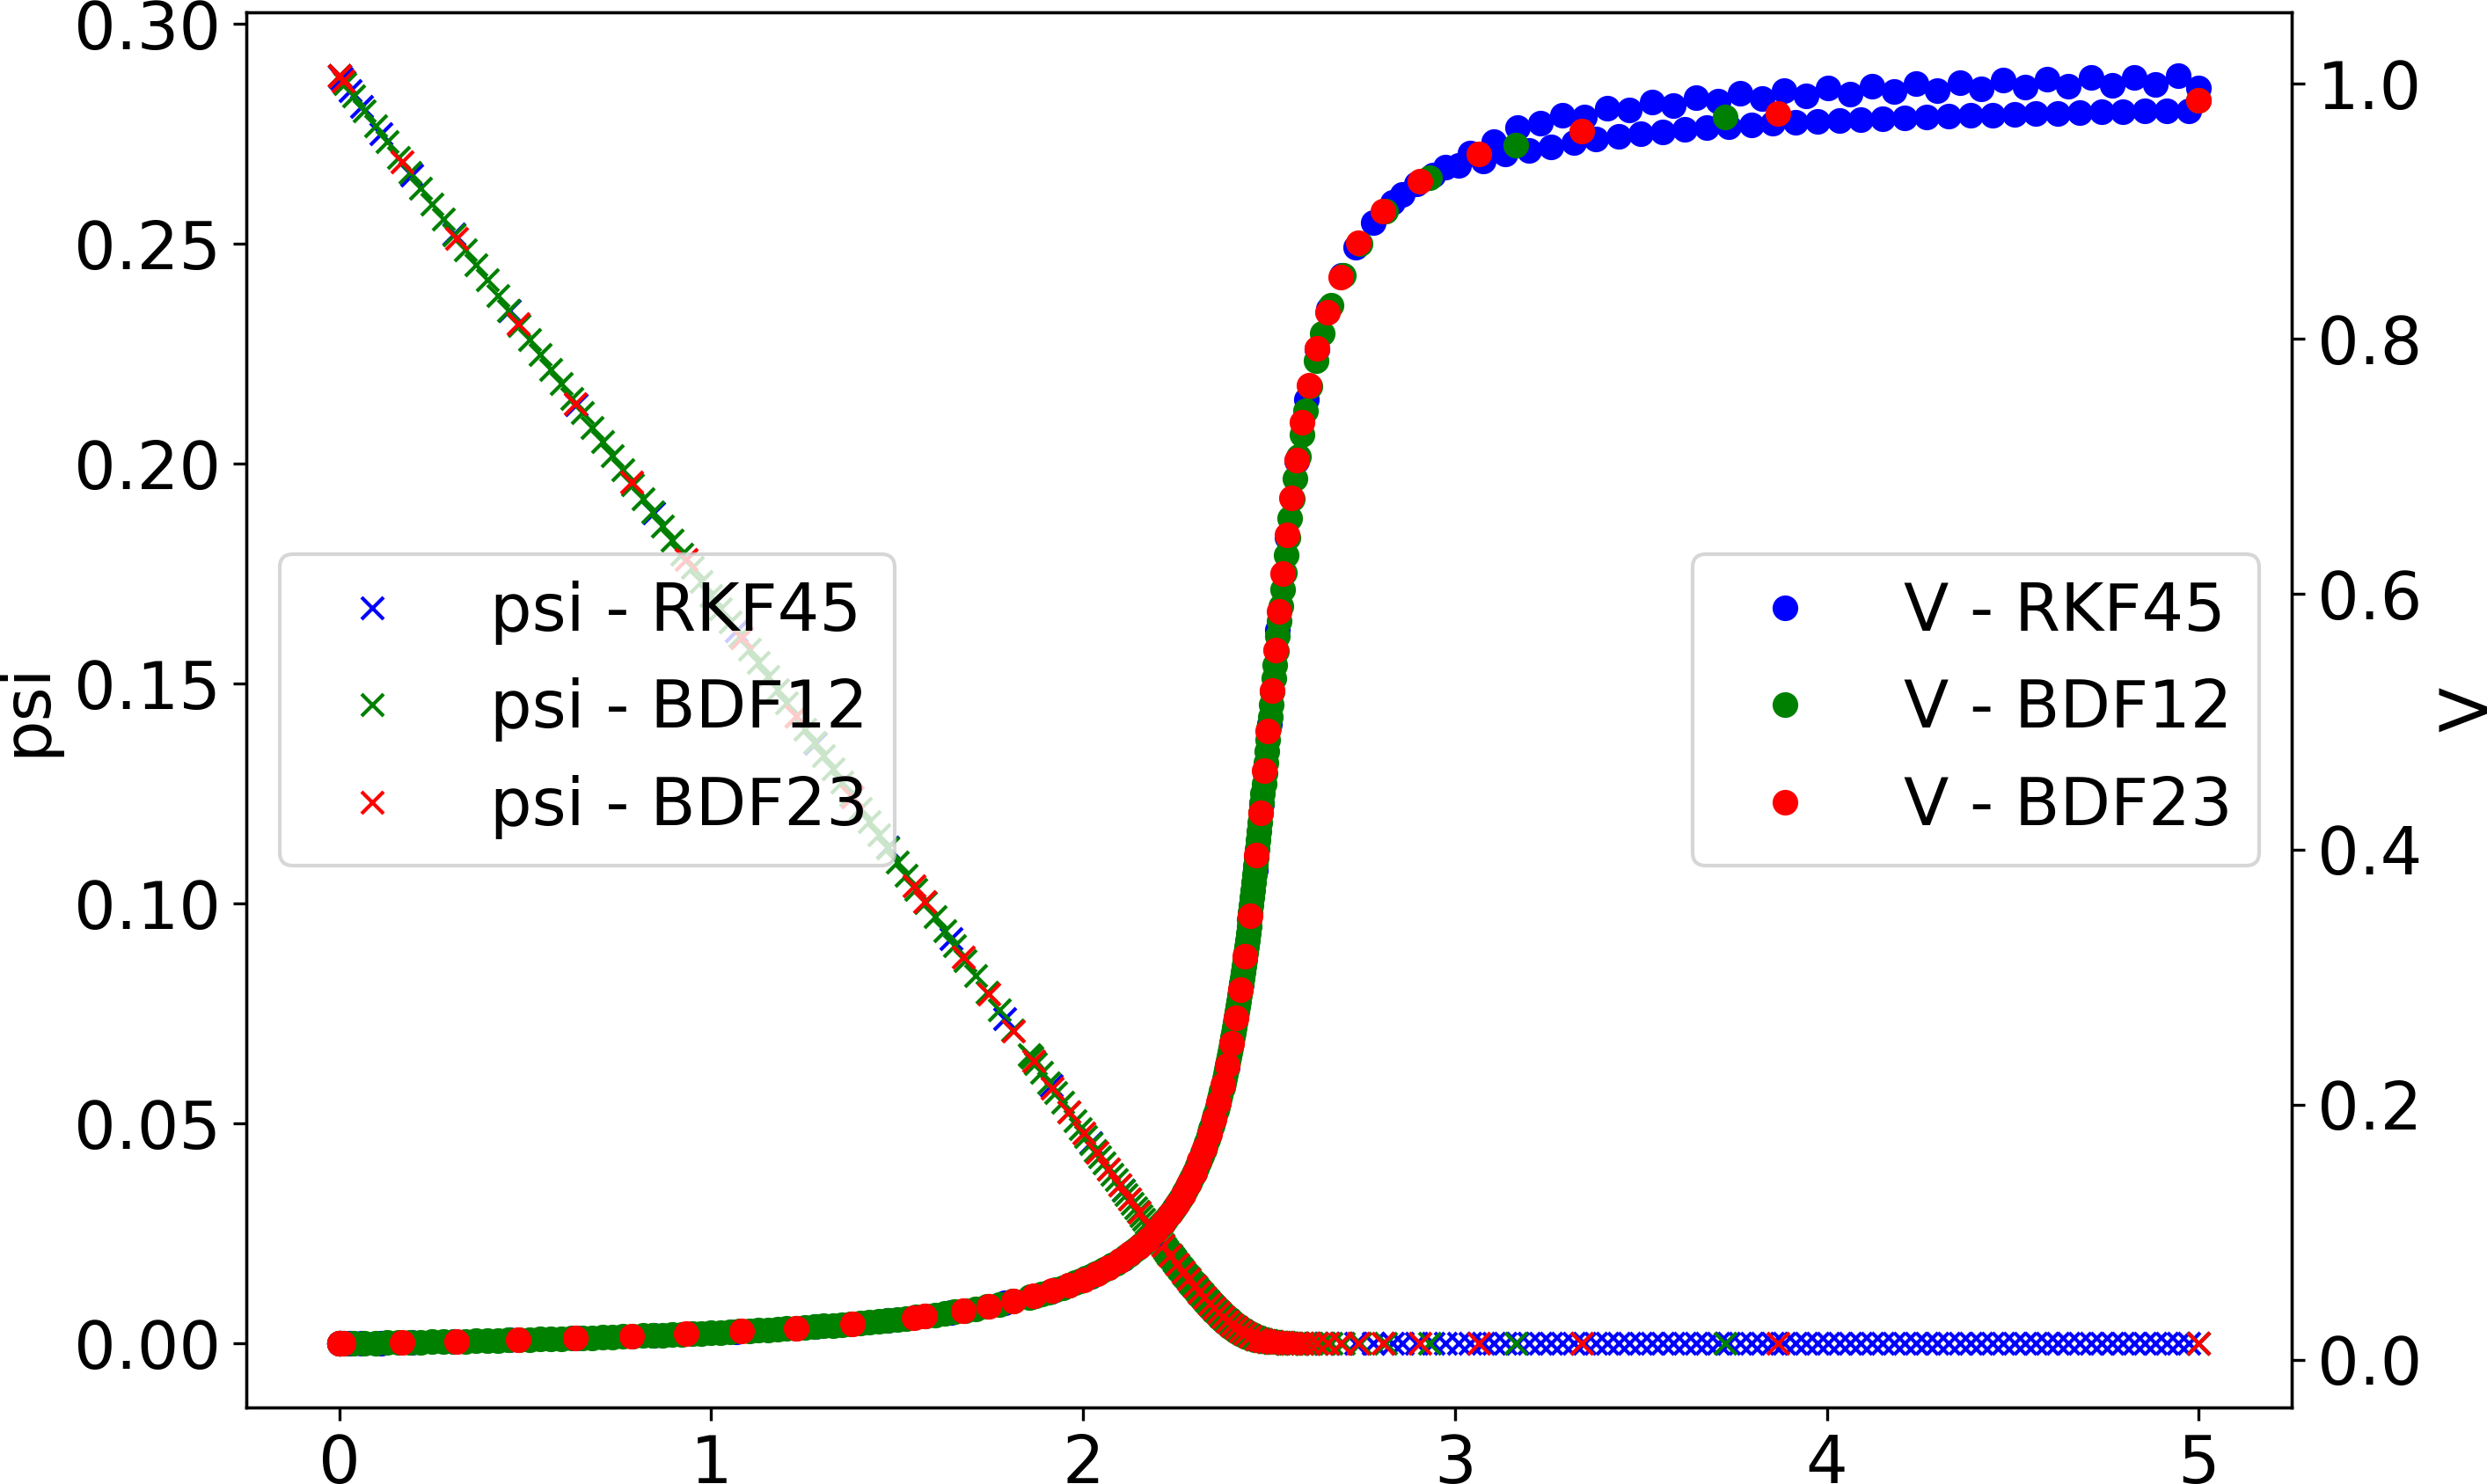
\includegraphics[width=1\textwidth]{images/timeEvolutionValues.png}
       	\subcaption{Evolution of the velocity $V$ and of the state variable $\psi$} 
        \label{fig:timeEvolutionValues}
    \end{subfigure}
    \begin{subfigure}{0.43\textwidth}
    	\centering
    	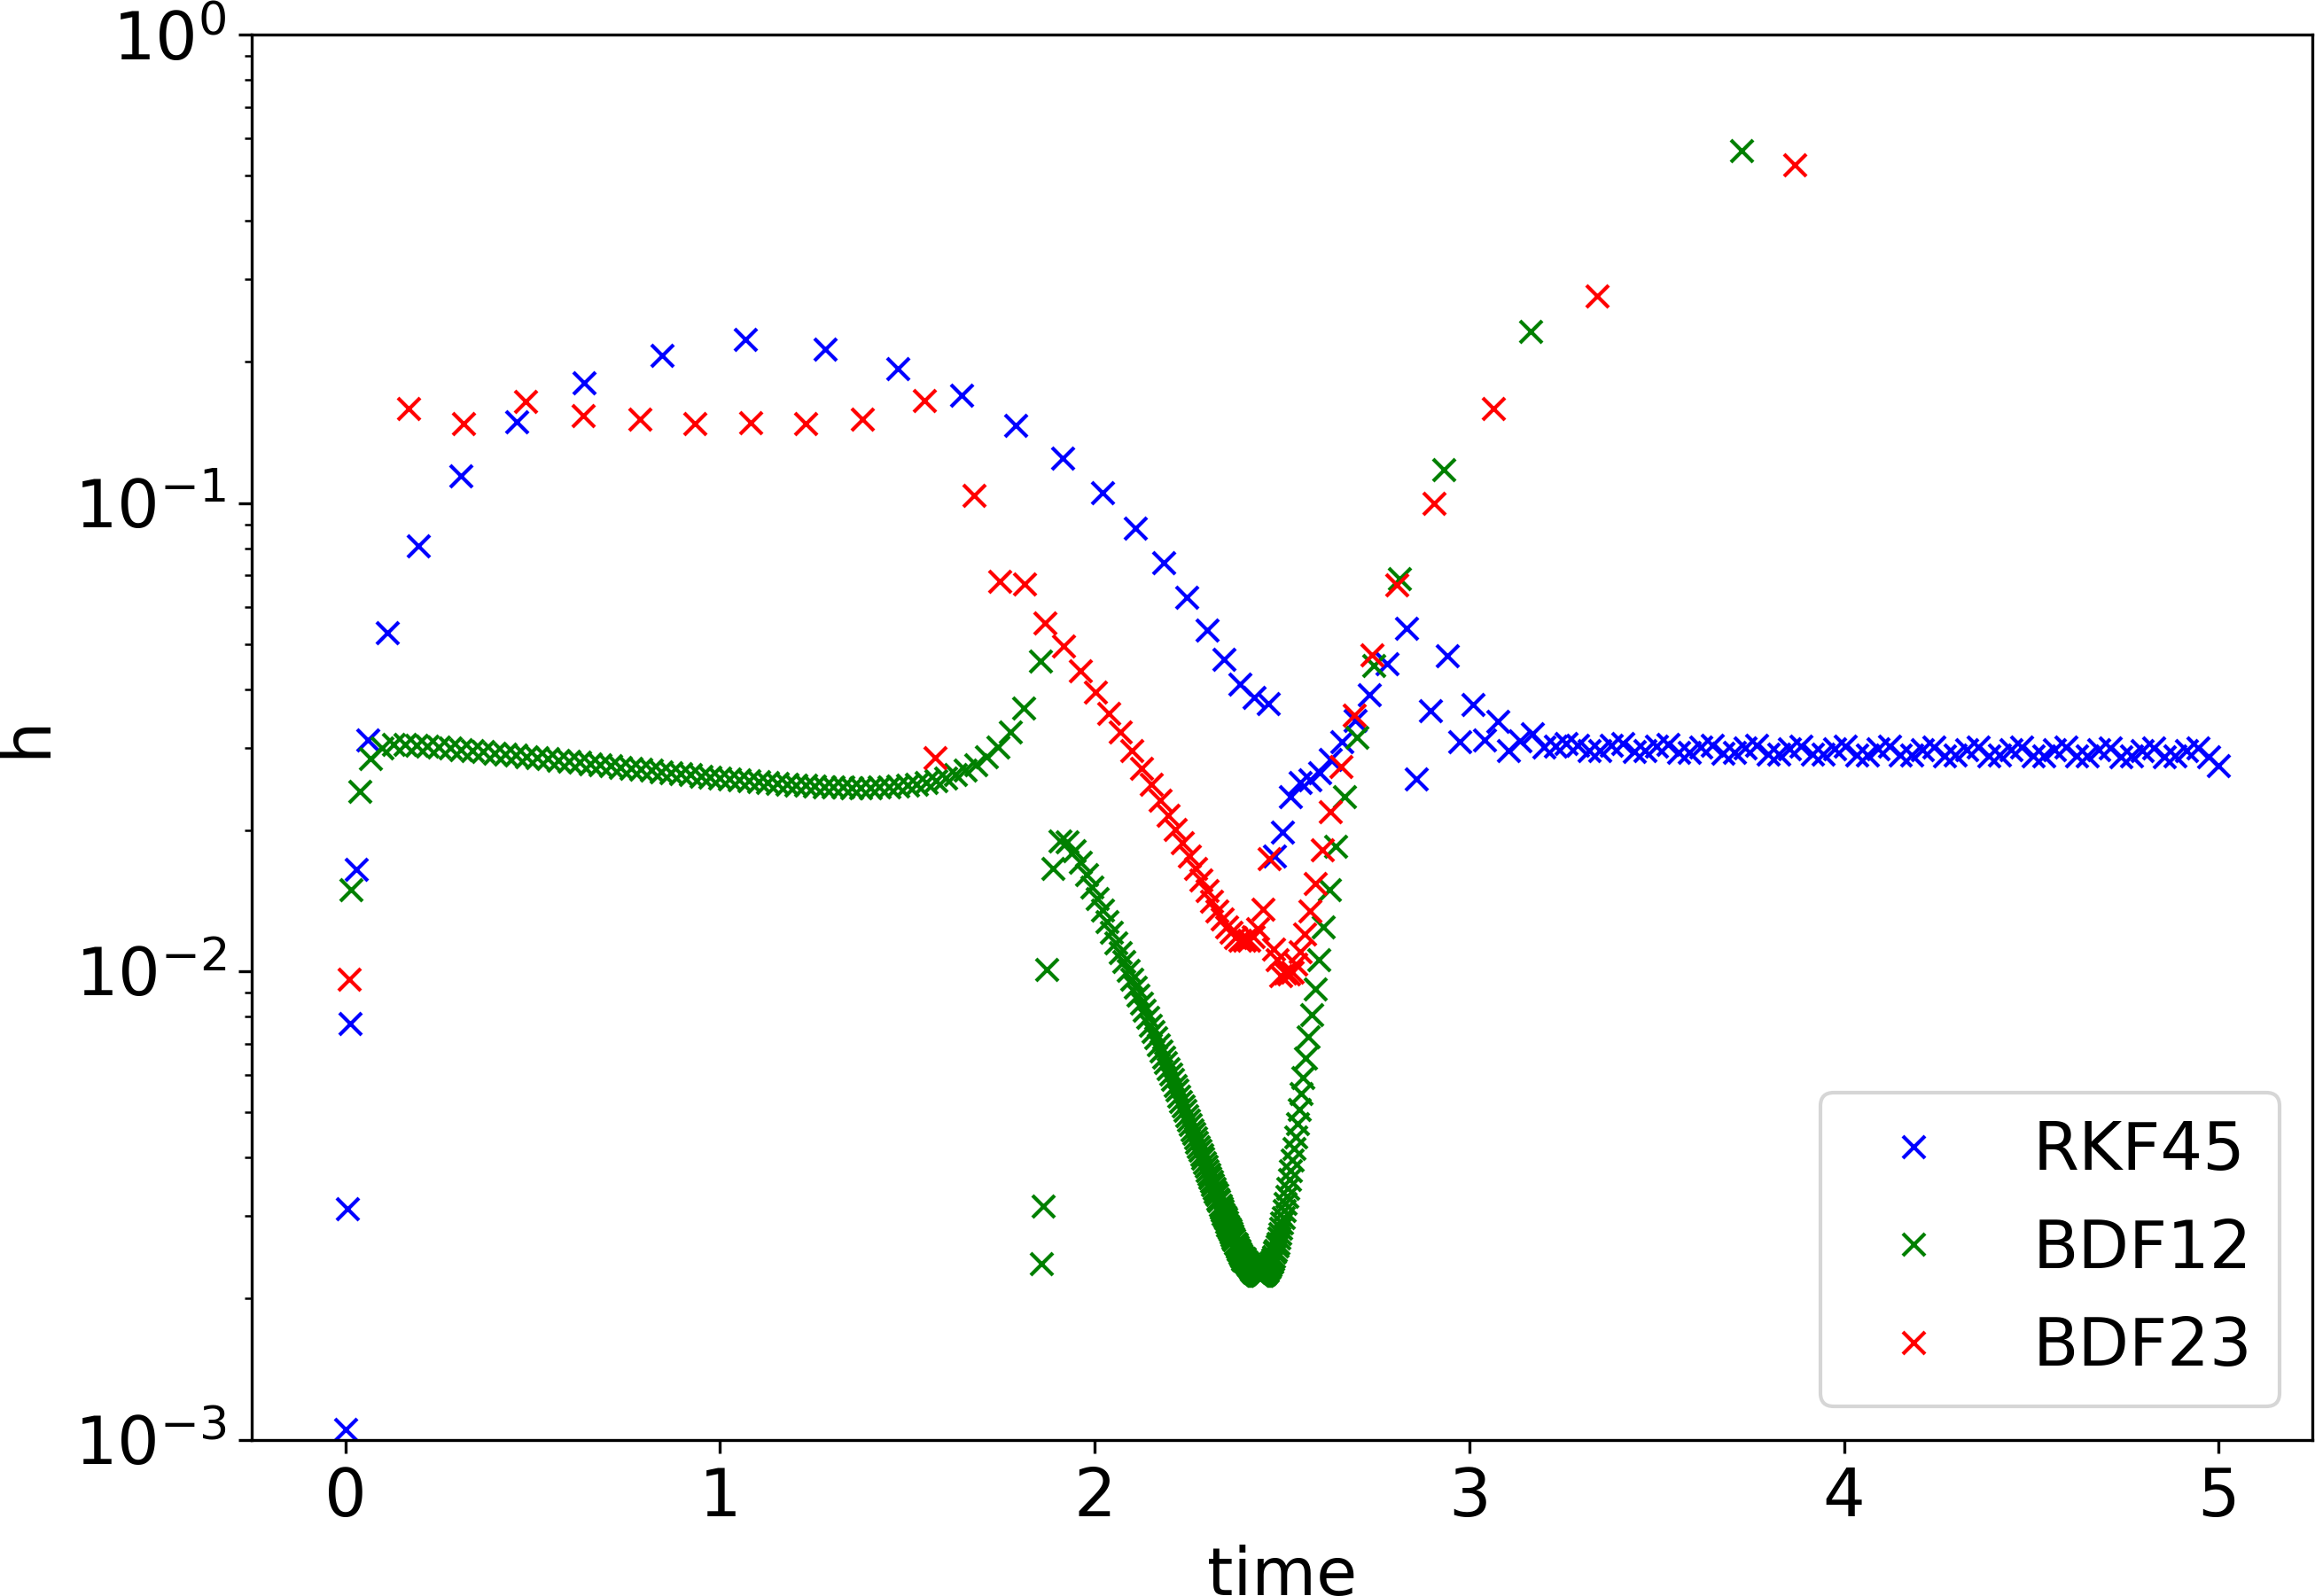
\includegraphics[width=1\textwidth]{images/timeEvolutionDT.png}
       	\subcaption{Evolution of the timestep size $h_n$} 
        \label{fig:timeEvolutionDT}
    \end{subfigure}
    \caption{Evolution of the solution and the timestep sizes of the single state problem defined in \autoref{eq:first_DAE_algeb} with the implemented numerical schemes}
\end{figure}

Now, the accuracy of the three numerical methods is compared. Therefore, \autoref{fig:timeEvolutionErrorPSI} depicts the evolution of the absolute difference between the numerical solution and the analytical solution of the state variable $\psi$. It is of interest to compare this error with the absolute error in velocity, shown in \autoref{fig:timeEvolutionVerror}. \\ 
As $\psi$ decreases, the error in $\psi$ increases steadily for all three numerical solvers. The implicit BDF methods produce two peaks in the evolution of the error, the first shortly before the end of the decrease and the second at the stiff transition of the velocity from 0 to 1. The norm of the error is much higher for BDF12 than for BDF23, despite the lower number of timesteps of the latter. The explicit RKF45 method produces a similar error norm as BDF12, but only in one peak at the beginning of the transition phase. In the end of the simulation, when $\psi$ stays around 0, all solvers match closely with the analytical solution and the error remains very low. On the other hand, the error in the velocity is very low for all solvers at the beginning and a peak in the error appears at the transition from 0 to 1. As usual, the highest error here appears for BDF12. Between the two remaining methods, RKF45 has the lowest error, which is astonishing for an explicit method applied to a stiff problem, especially considering the fact that in this section of the simulations, it also allows larger timesteps. Towards the end of the simulation, the error in velocity obtained by the two implicit methods vanishes again, however RKF45 produces suddenly very high errors which alternate between three different values. In \autoref{fig:timeEvolutionValues}, it can be seen that the velocity oscillates around the expected solution without getting closer to it. \\
It is important to realise that the error in $\psi$ and in the velocity are not directly correlated, thus a small error in $\psi$ does not necessarily lead to a small error in the velocity. It might thus be wise to reconsider the way the timestep size is controlled. So far, it only depends on the ratio between the local truncation error and a predefined tolerance value. This error is estimated by applying another numerical scheme with higher order, by taking the difference in $\psi$ of the two solutions as error estimate. Therefore, the velocity is not involved in the step size controller and the controller cannot ensure that the chosen timestep size guarantees sufficiently accurate results for the velocity. To ensure correct physical results, the controller needs to be extended in a way to restrict the timestep size with respect to some error estimate of the velocity. 

\begin{figure}[H]
    \centering
    \begin{subfigure}{0.43\textwidth}
    	\centering
    	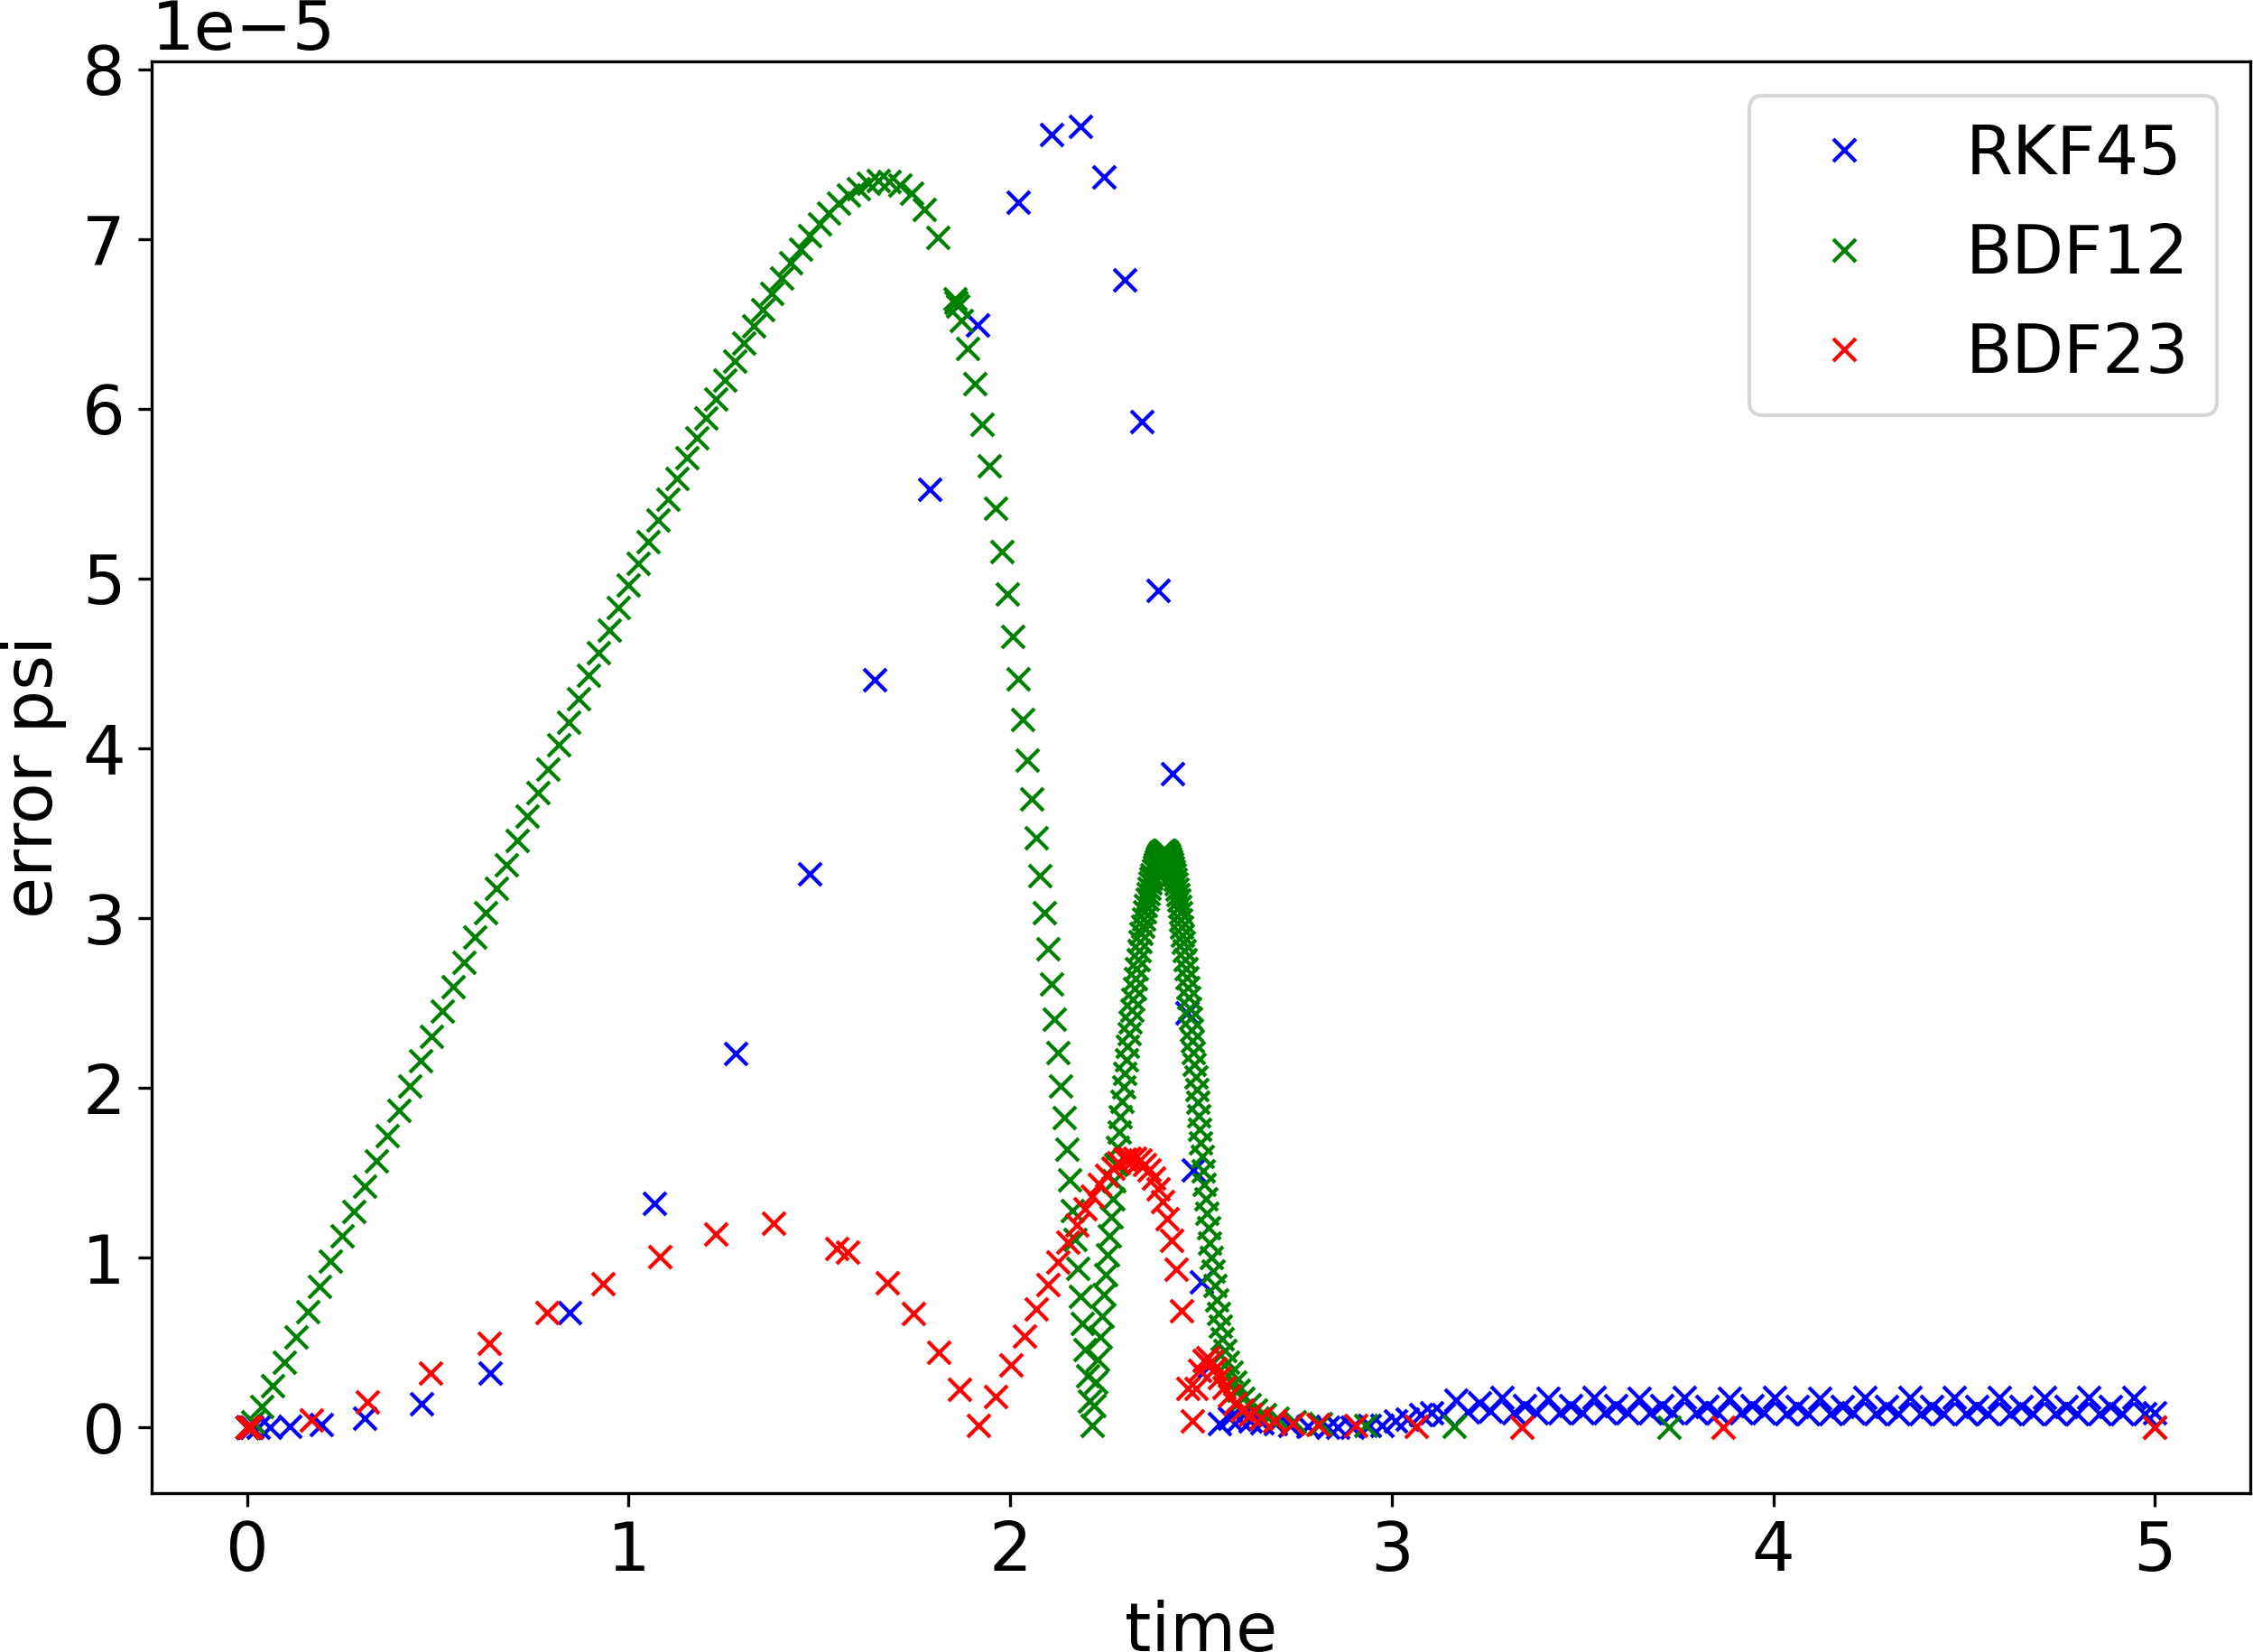
\includegraphics[width=1\textwidth]{images/timeEvolutionPSIerror.png}
       	\subcaption{Evolution of the absolute error of the state variable $\psi$} 
        \label{fig:timeEvolutionErrorPSI}
    \end{subfigure}
    \begin{subfigure}{0.43\textwidth}
    	\centering
    	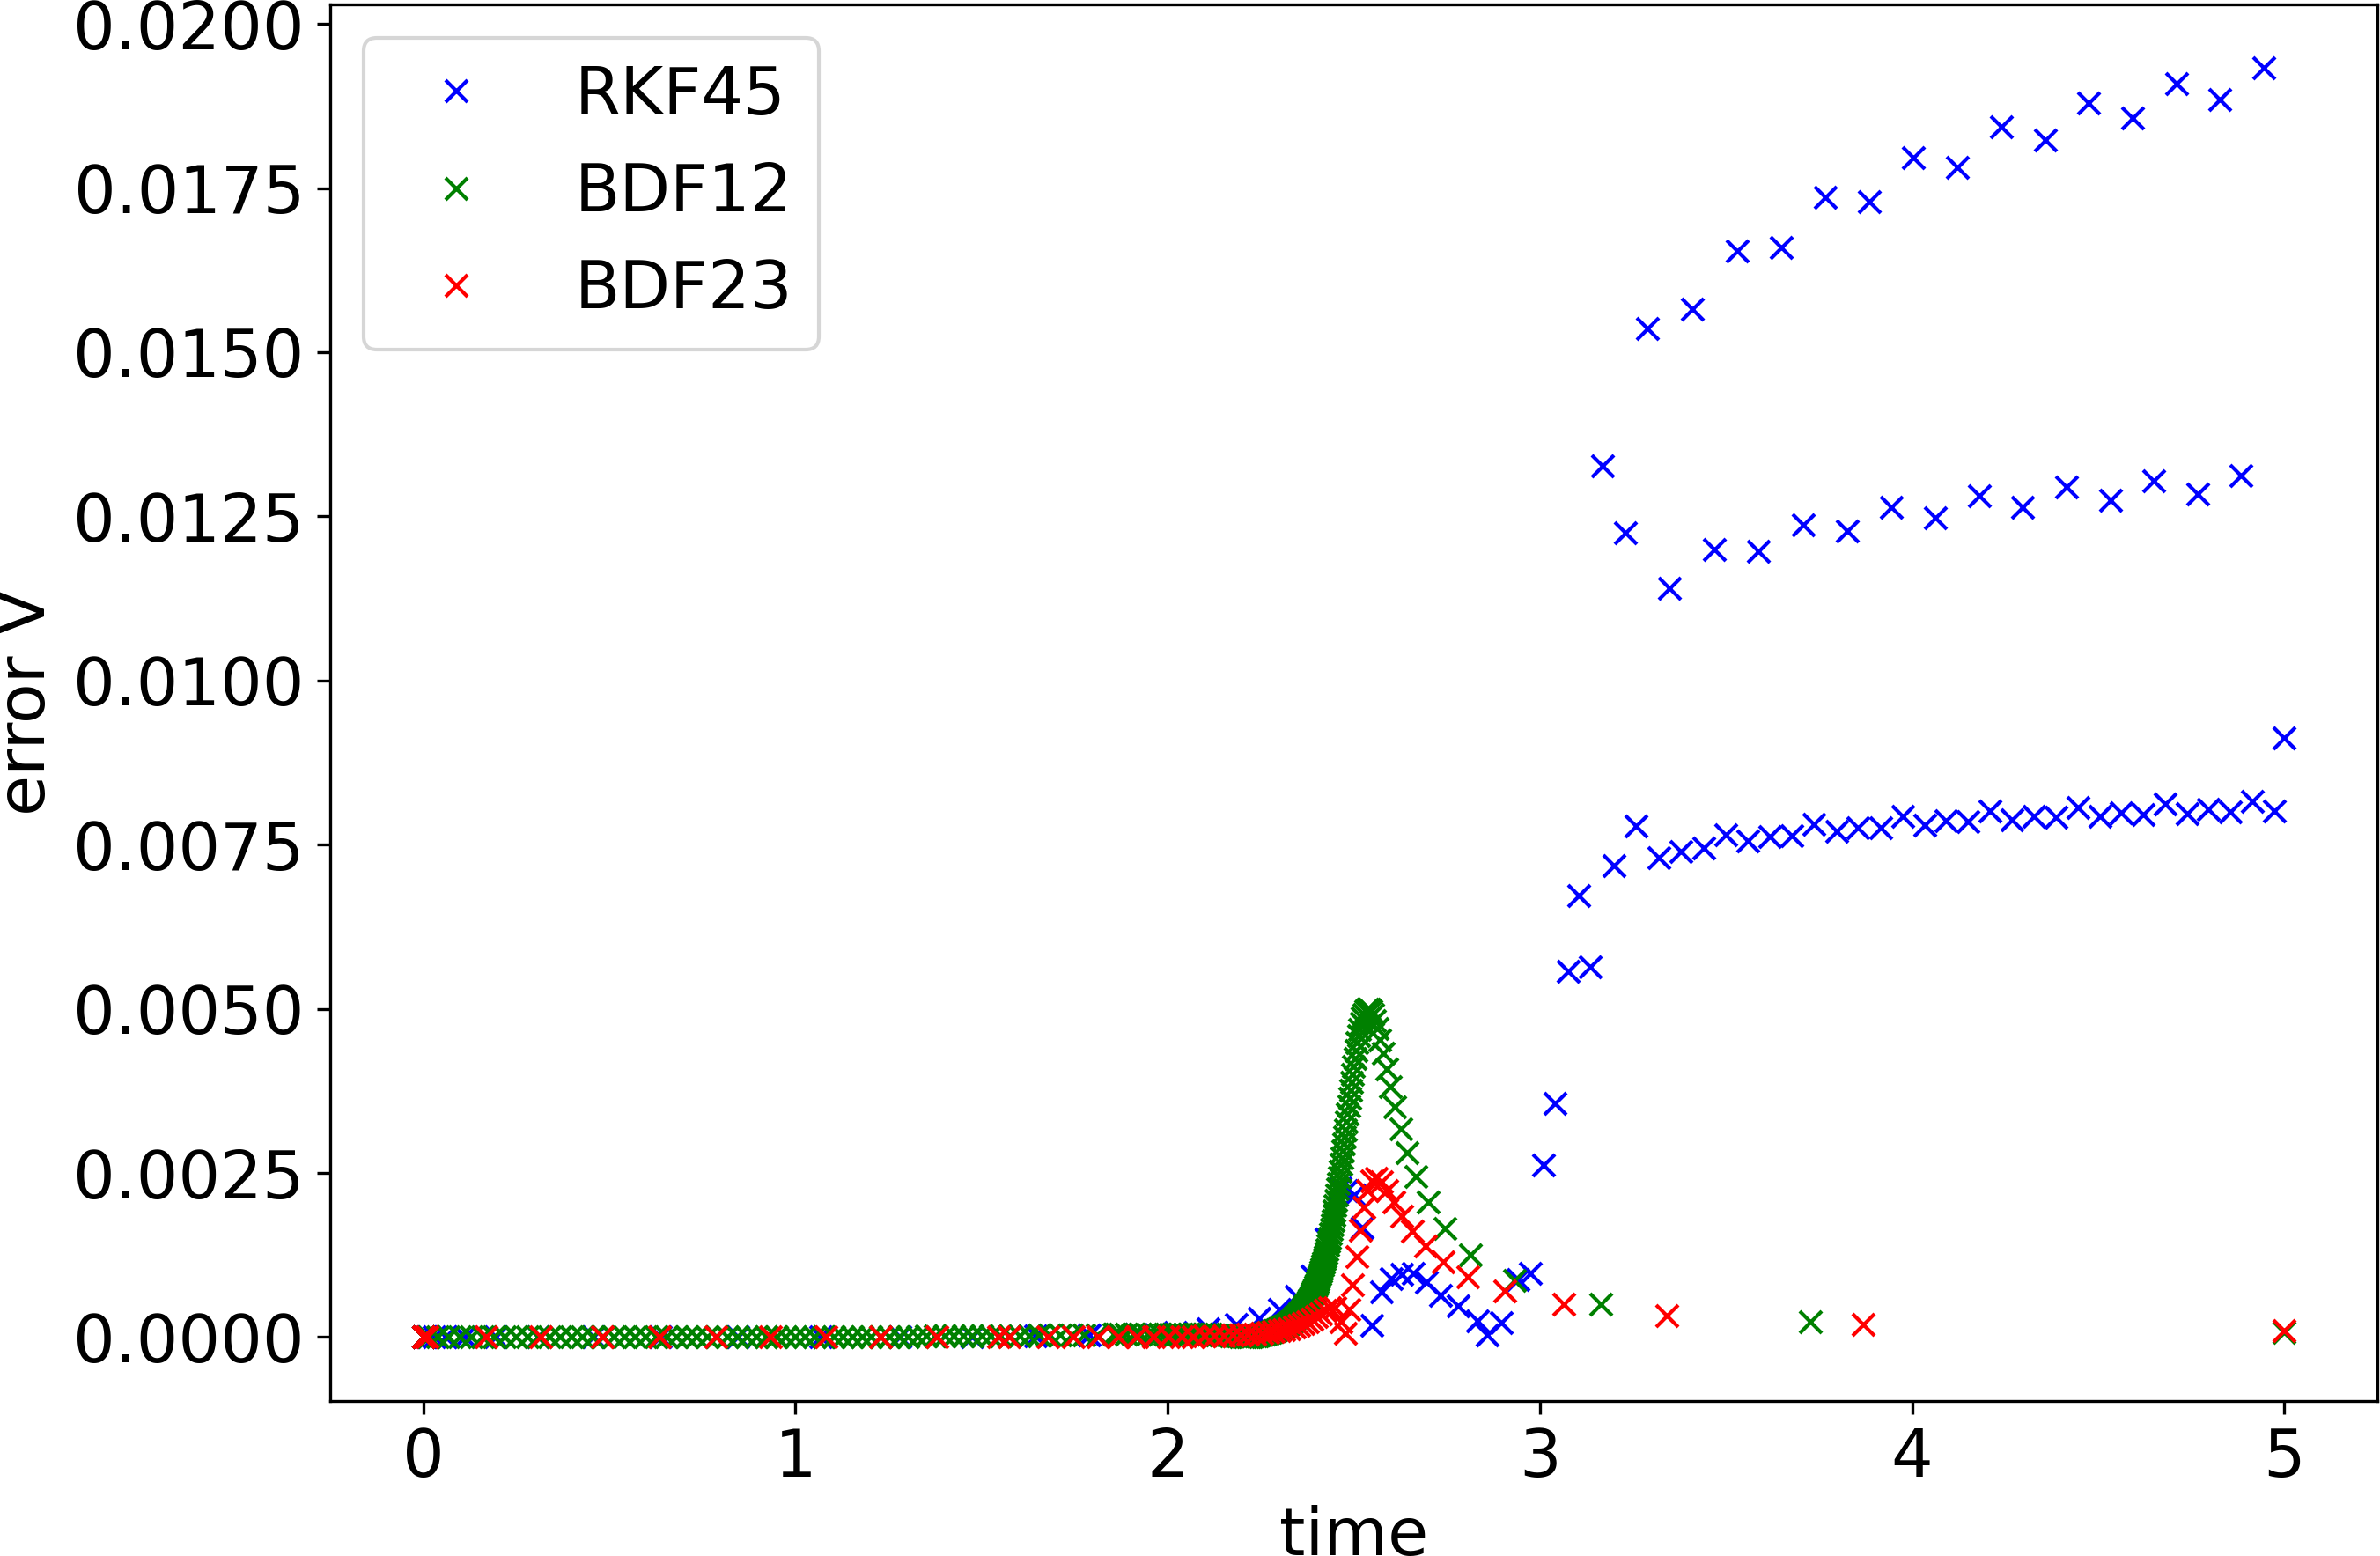
\includegraphics[width=1\textwidth]{images/timeEvolutionVerror.png}
       	\subcaption{Evolution of the absolute error of the velocity $V$} 
        \label{fig:timeEvolutionVerror}
    \end{subfigure}
    \caption{Evolution of the error for the single state problem defined in \autoref{eq:first_DAE_algeb} with the implemented numerical schemes}
\end{figure}

\subsection{Quality of the error estimates}
\label{ssec:QualityErrorEstimate_0D}
The whole theory of PI controller bases on an accurate error estimate, which is obtained in our case by calculating the solution with a higher order method. It is interesting to analyze whether the error estimate calculated in this way matches with the actual error to the analytical solution. The absolute error cannot be used as in the previous graphs, since the error estimate is calculated from the lower-order solution at the previous timestep. On the other hand, the local truncation error, which measures by how much the total error increases at each timestep, is much better suited to evaluate the accuracy of the error estimate. \\
In \autoref{fig:errorEstimateEvolutionALL}, the difference between the two solutions calculated at each timestep by any of the schemes, being the error estimate, plotted against the real local truncation error. In the initial phase, the two implicit methods estimate the error very closely to its real value. Even though the BDF12 method approximates it better than the BDF23 method, the high amount of executed timesteps in this phase accumulate the total error which turns out to be much worse. The estimate of the explicit RKF45 method roughly follows the real evolution of the local truncation error, but underestimates it by a large factor up to 5. During the transition phase, the situation is reversed, because the implicit methods fail at estimating correctly peaks in the evolution of the real error and remain instead around a same value. On the other hand, the RKF45 follows much better the evolution of the local truncation error, which explains its good performance in the transition phase with respect to the allowed timestep size and to the total error. In the final phase, the two implicit methods match again with the expected error values and the RKF45 method seems to fit exactly the real error, but it shows nonphysical oscillations which seem to correspond to the larges oscillations in the total error of the velocity. \\
Overall, the implicit methods yield the better error estimates except for the stiff transition which seems to be better handled by the explicit scheme. 

\begin{figure}[H]
    \centering
    \begin{subfigure}{0.32\textwidth}
    	\centering
    	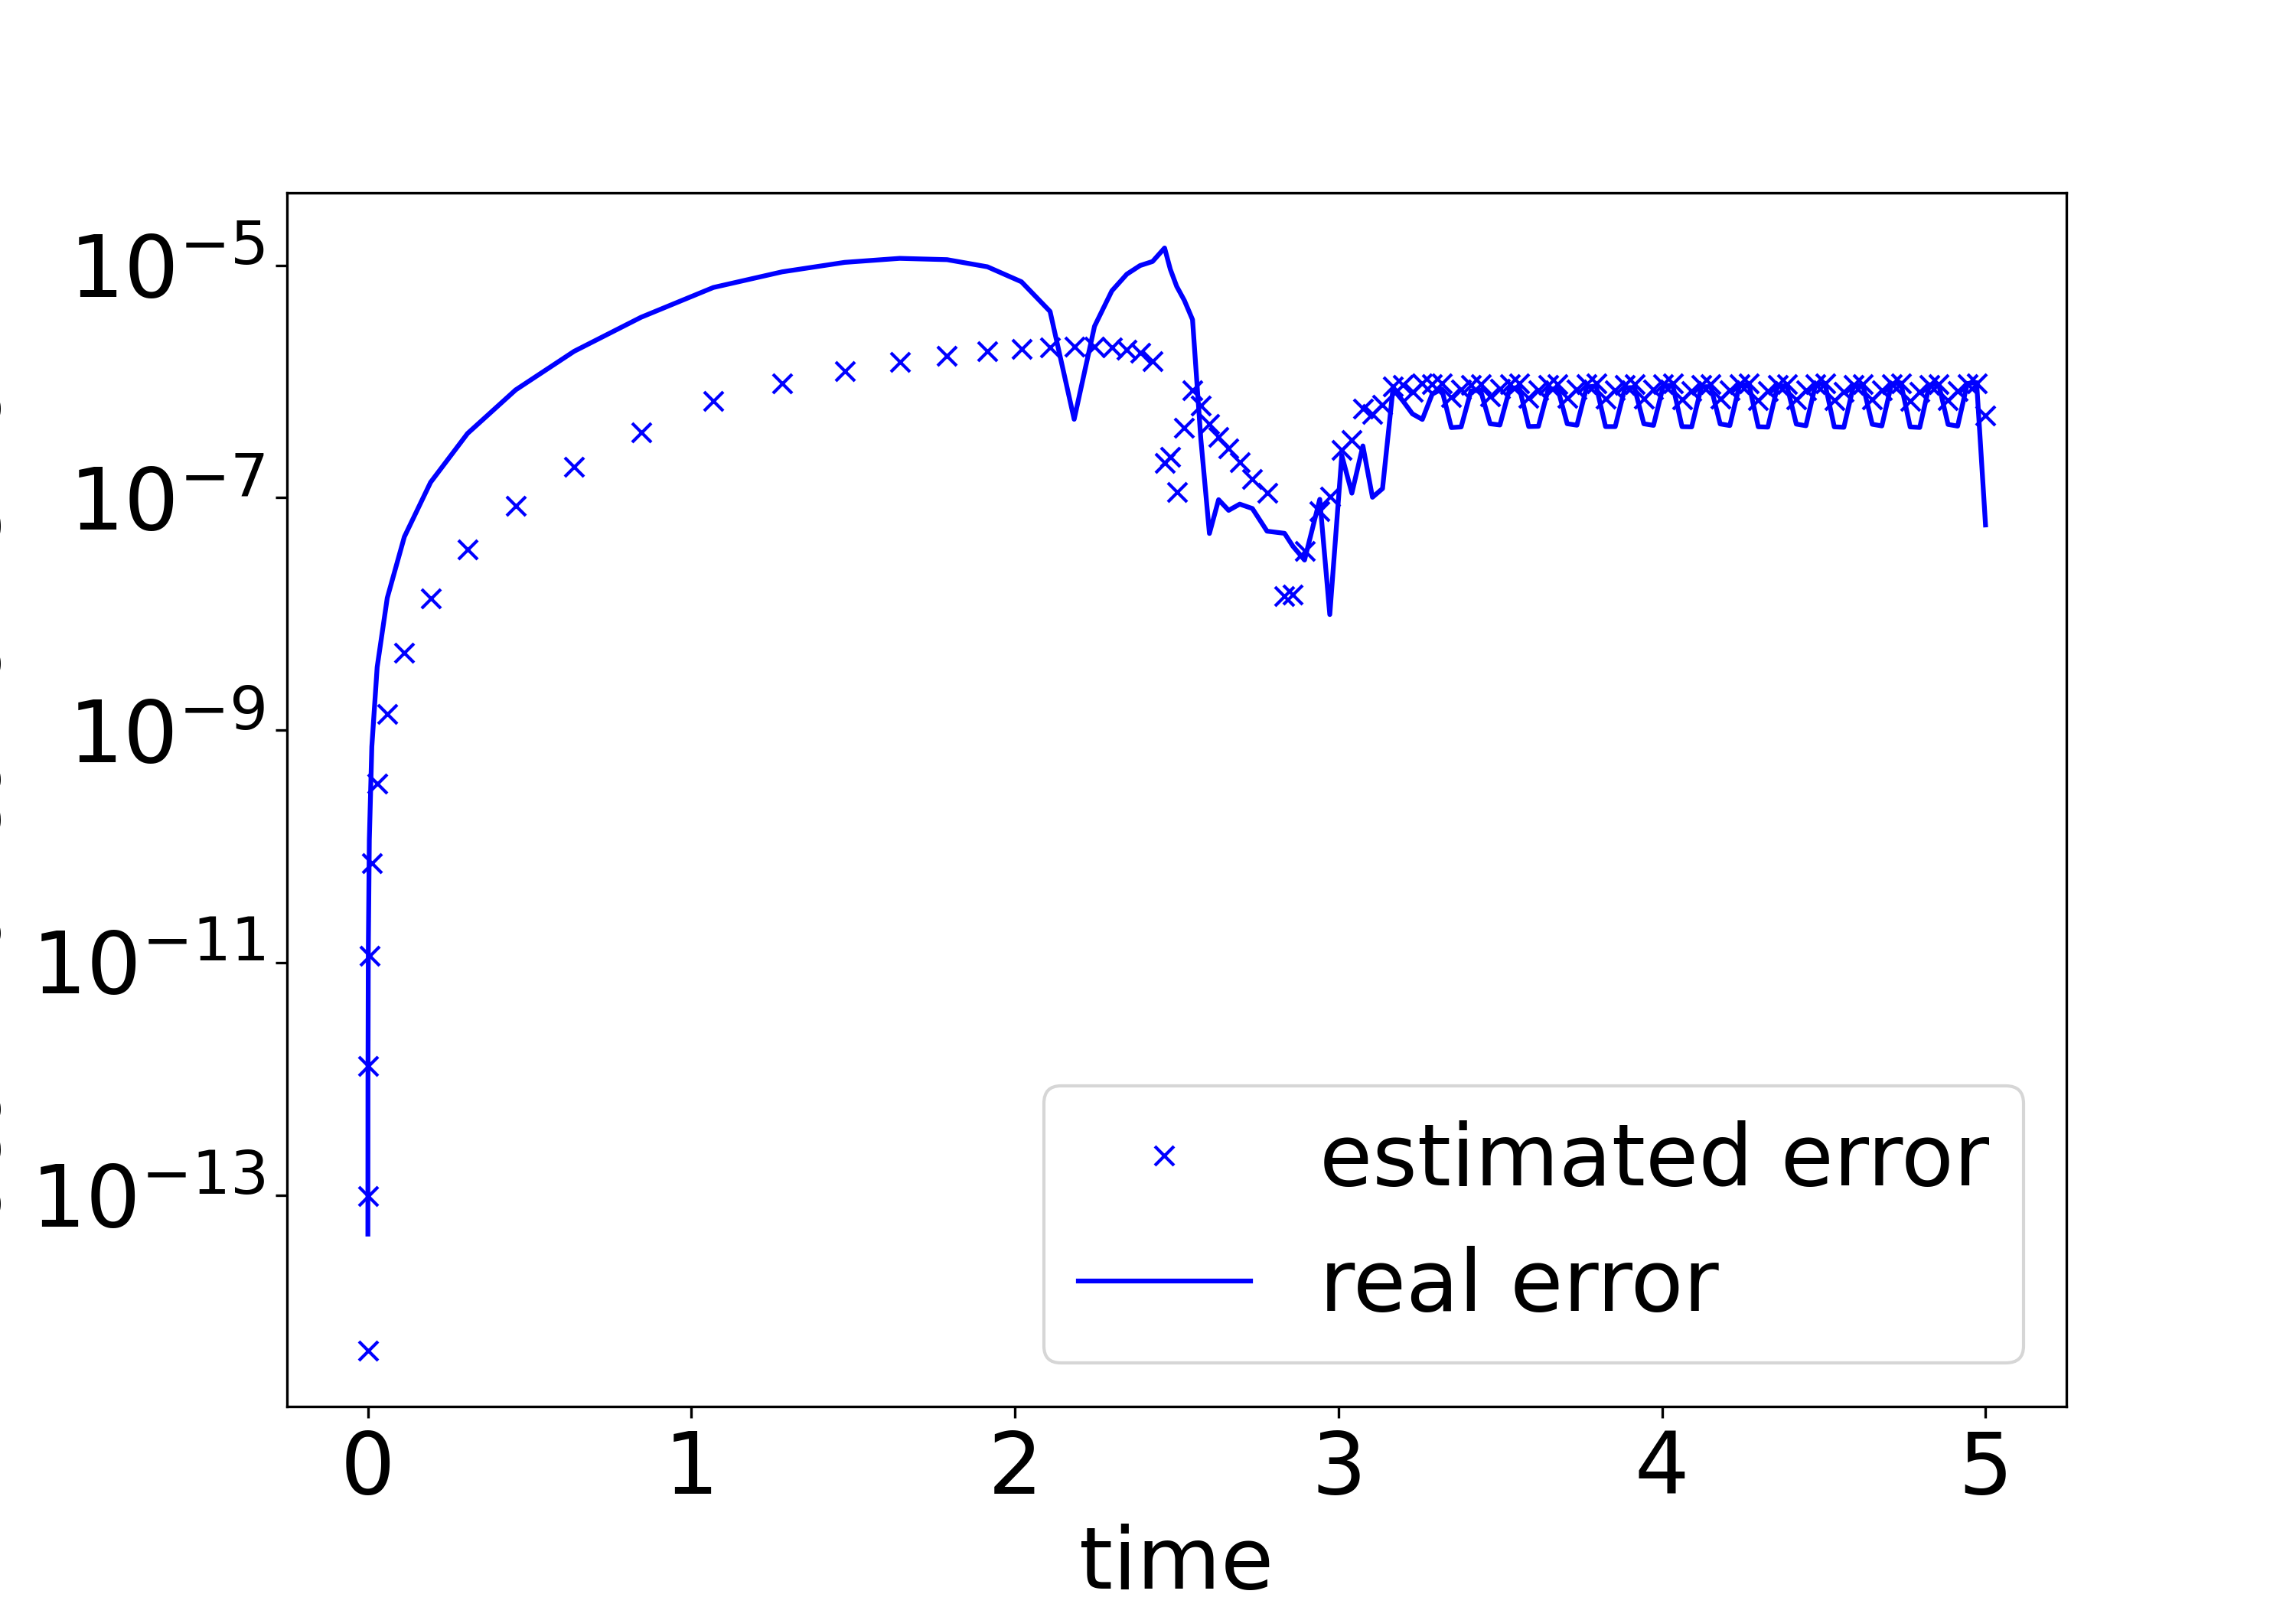
\includegraphics[width=1\textwidth]{images/errorEstimateRKF45.png}
       	\subcaption{\textbf{RKF45}} 
        \label{fig:errorEstimateEvolutionRKF45}
    \end{subfigure}
    \begin{subfigure}{0.32\textwidth}
    	\centering
    	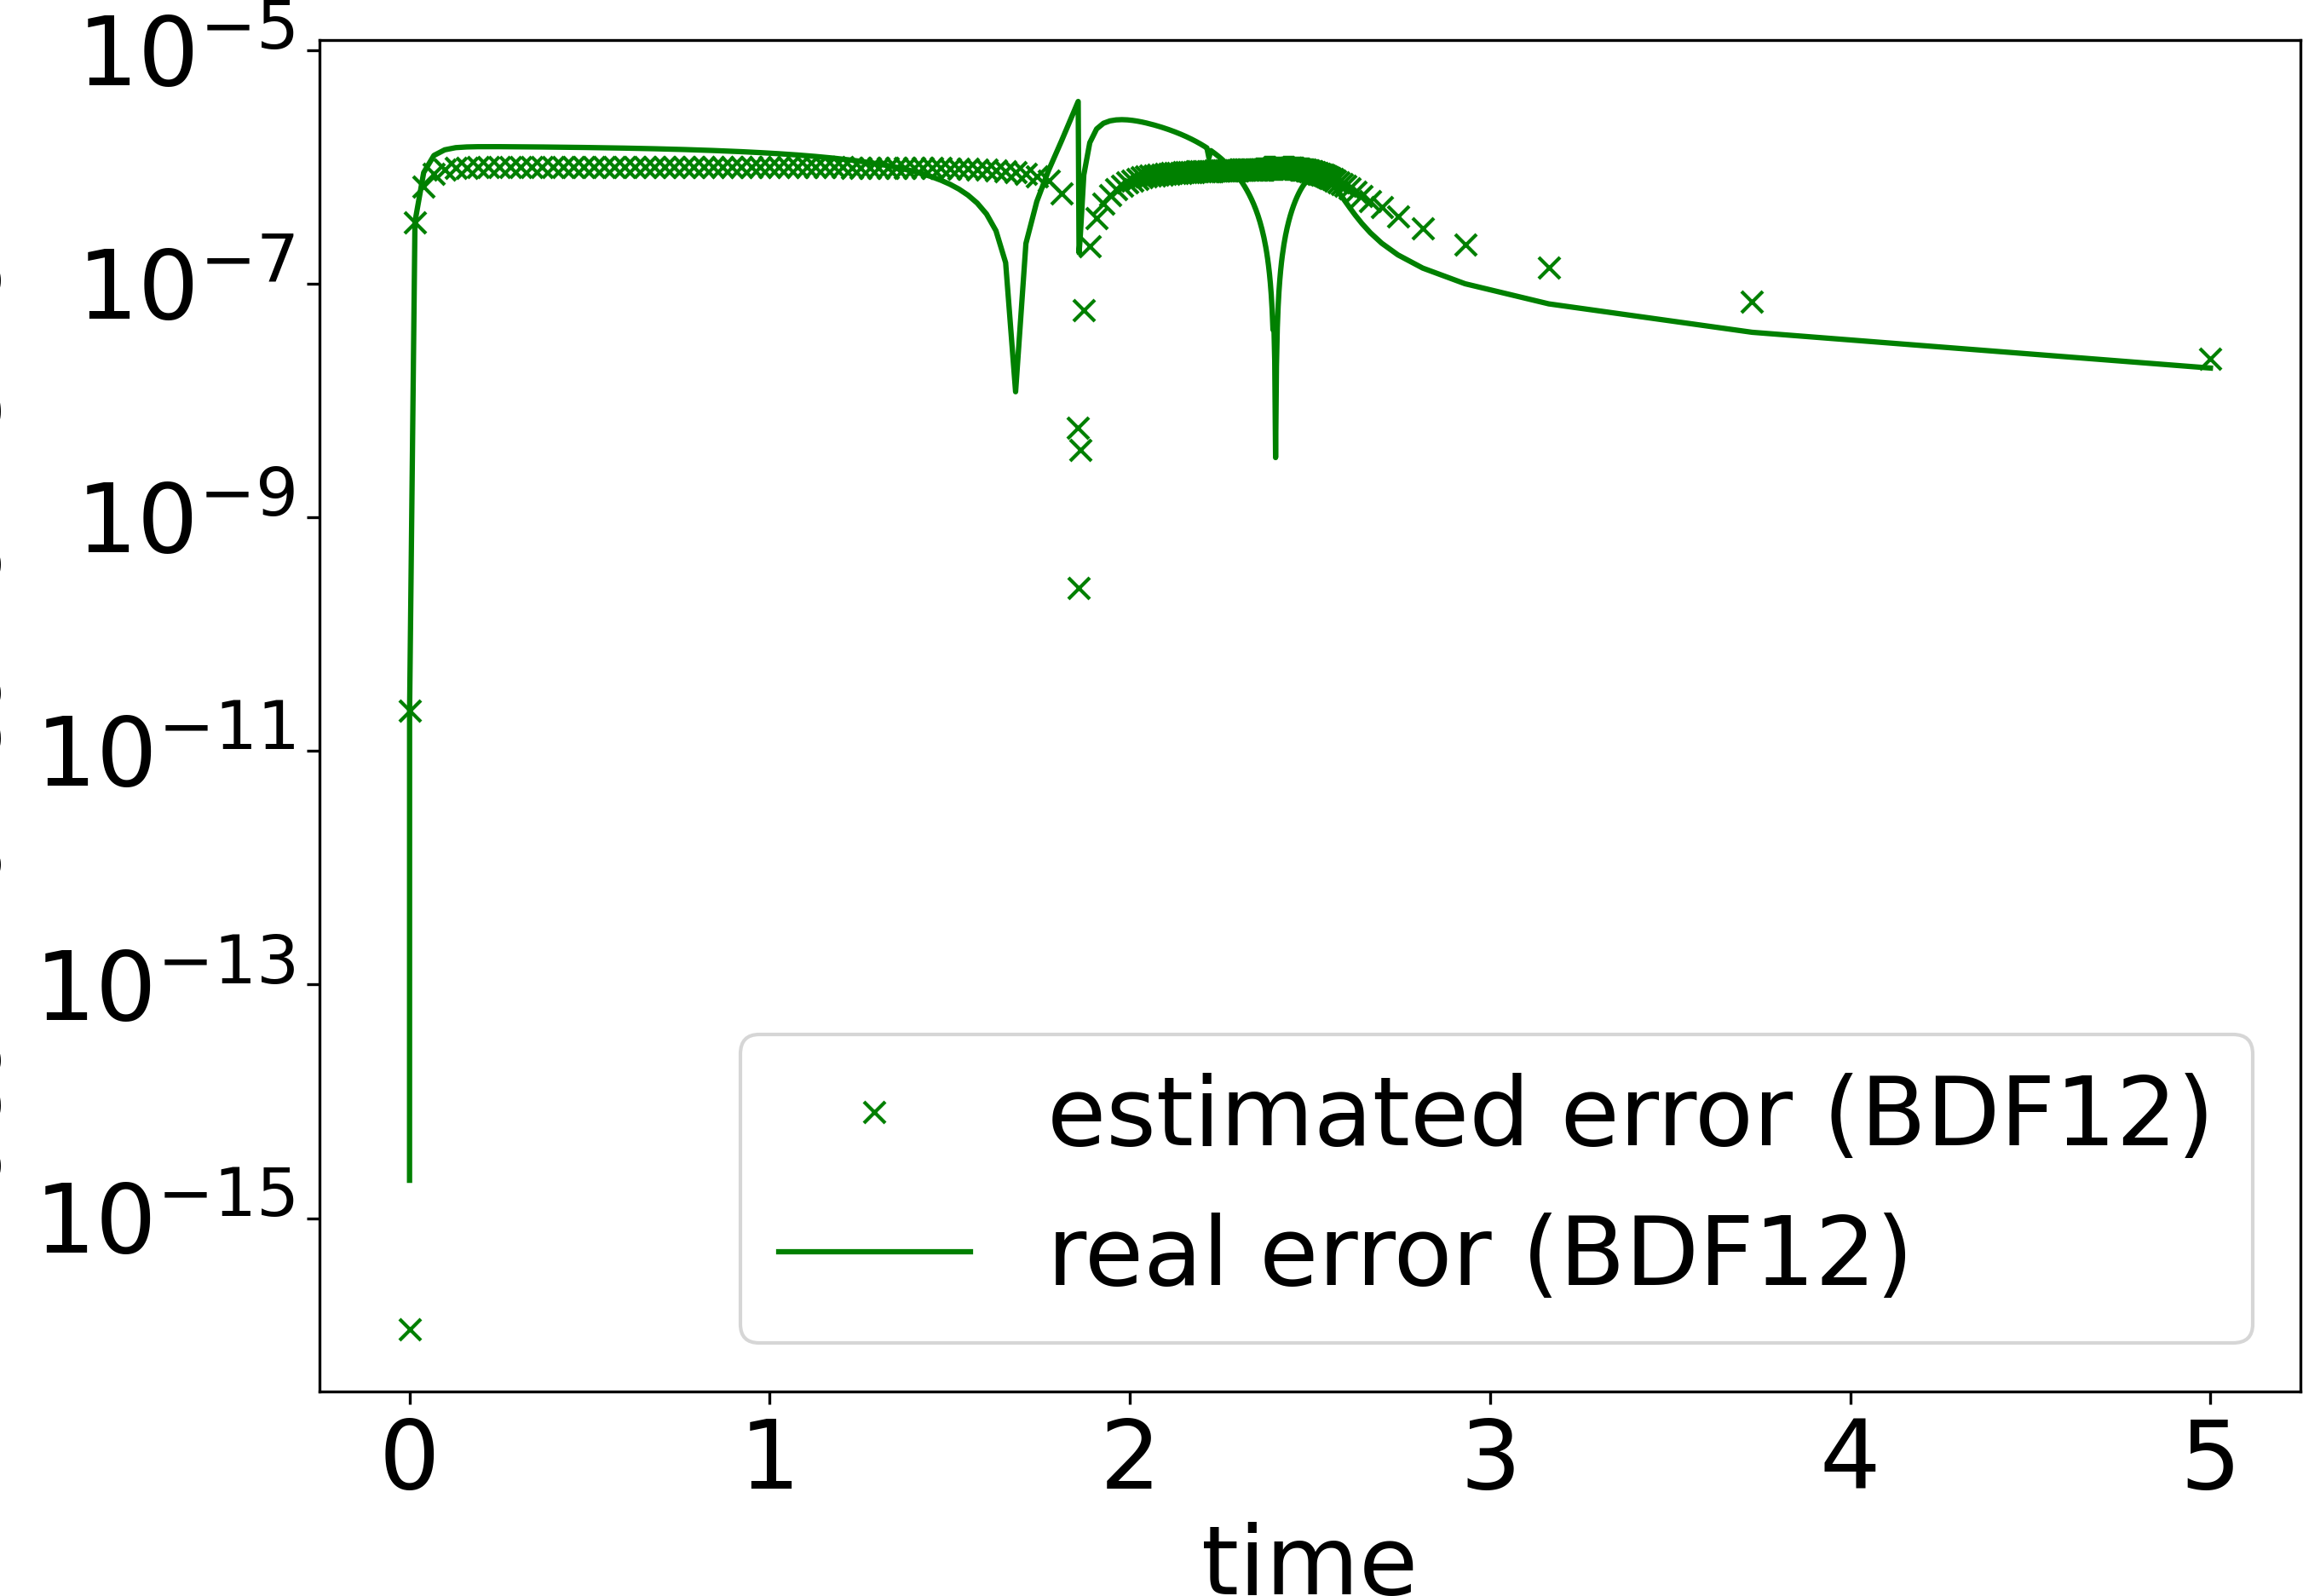
\includegraphics[width=1\textwidth]{images/errorEstimateBDF12.png}
       	\subcaption{\textbf{BDF12}} 
        \label{fig:errorEstimateEvolutionBDF12}
    \end{subfigure}
    \begin{subfigure}{0.32\textwidth}
    	\centering
    	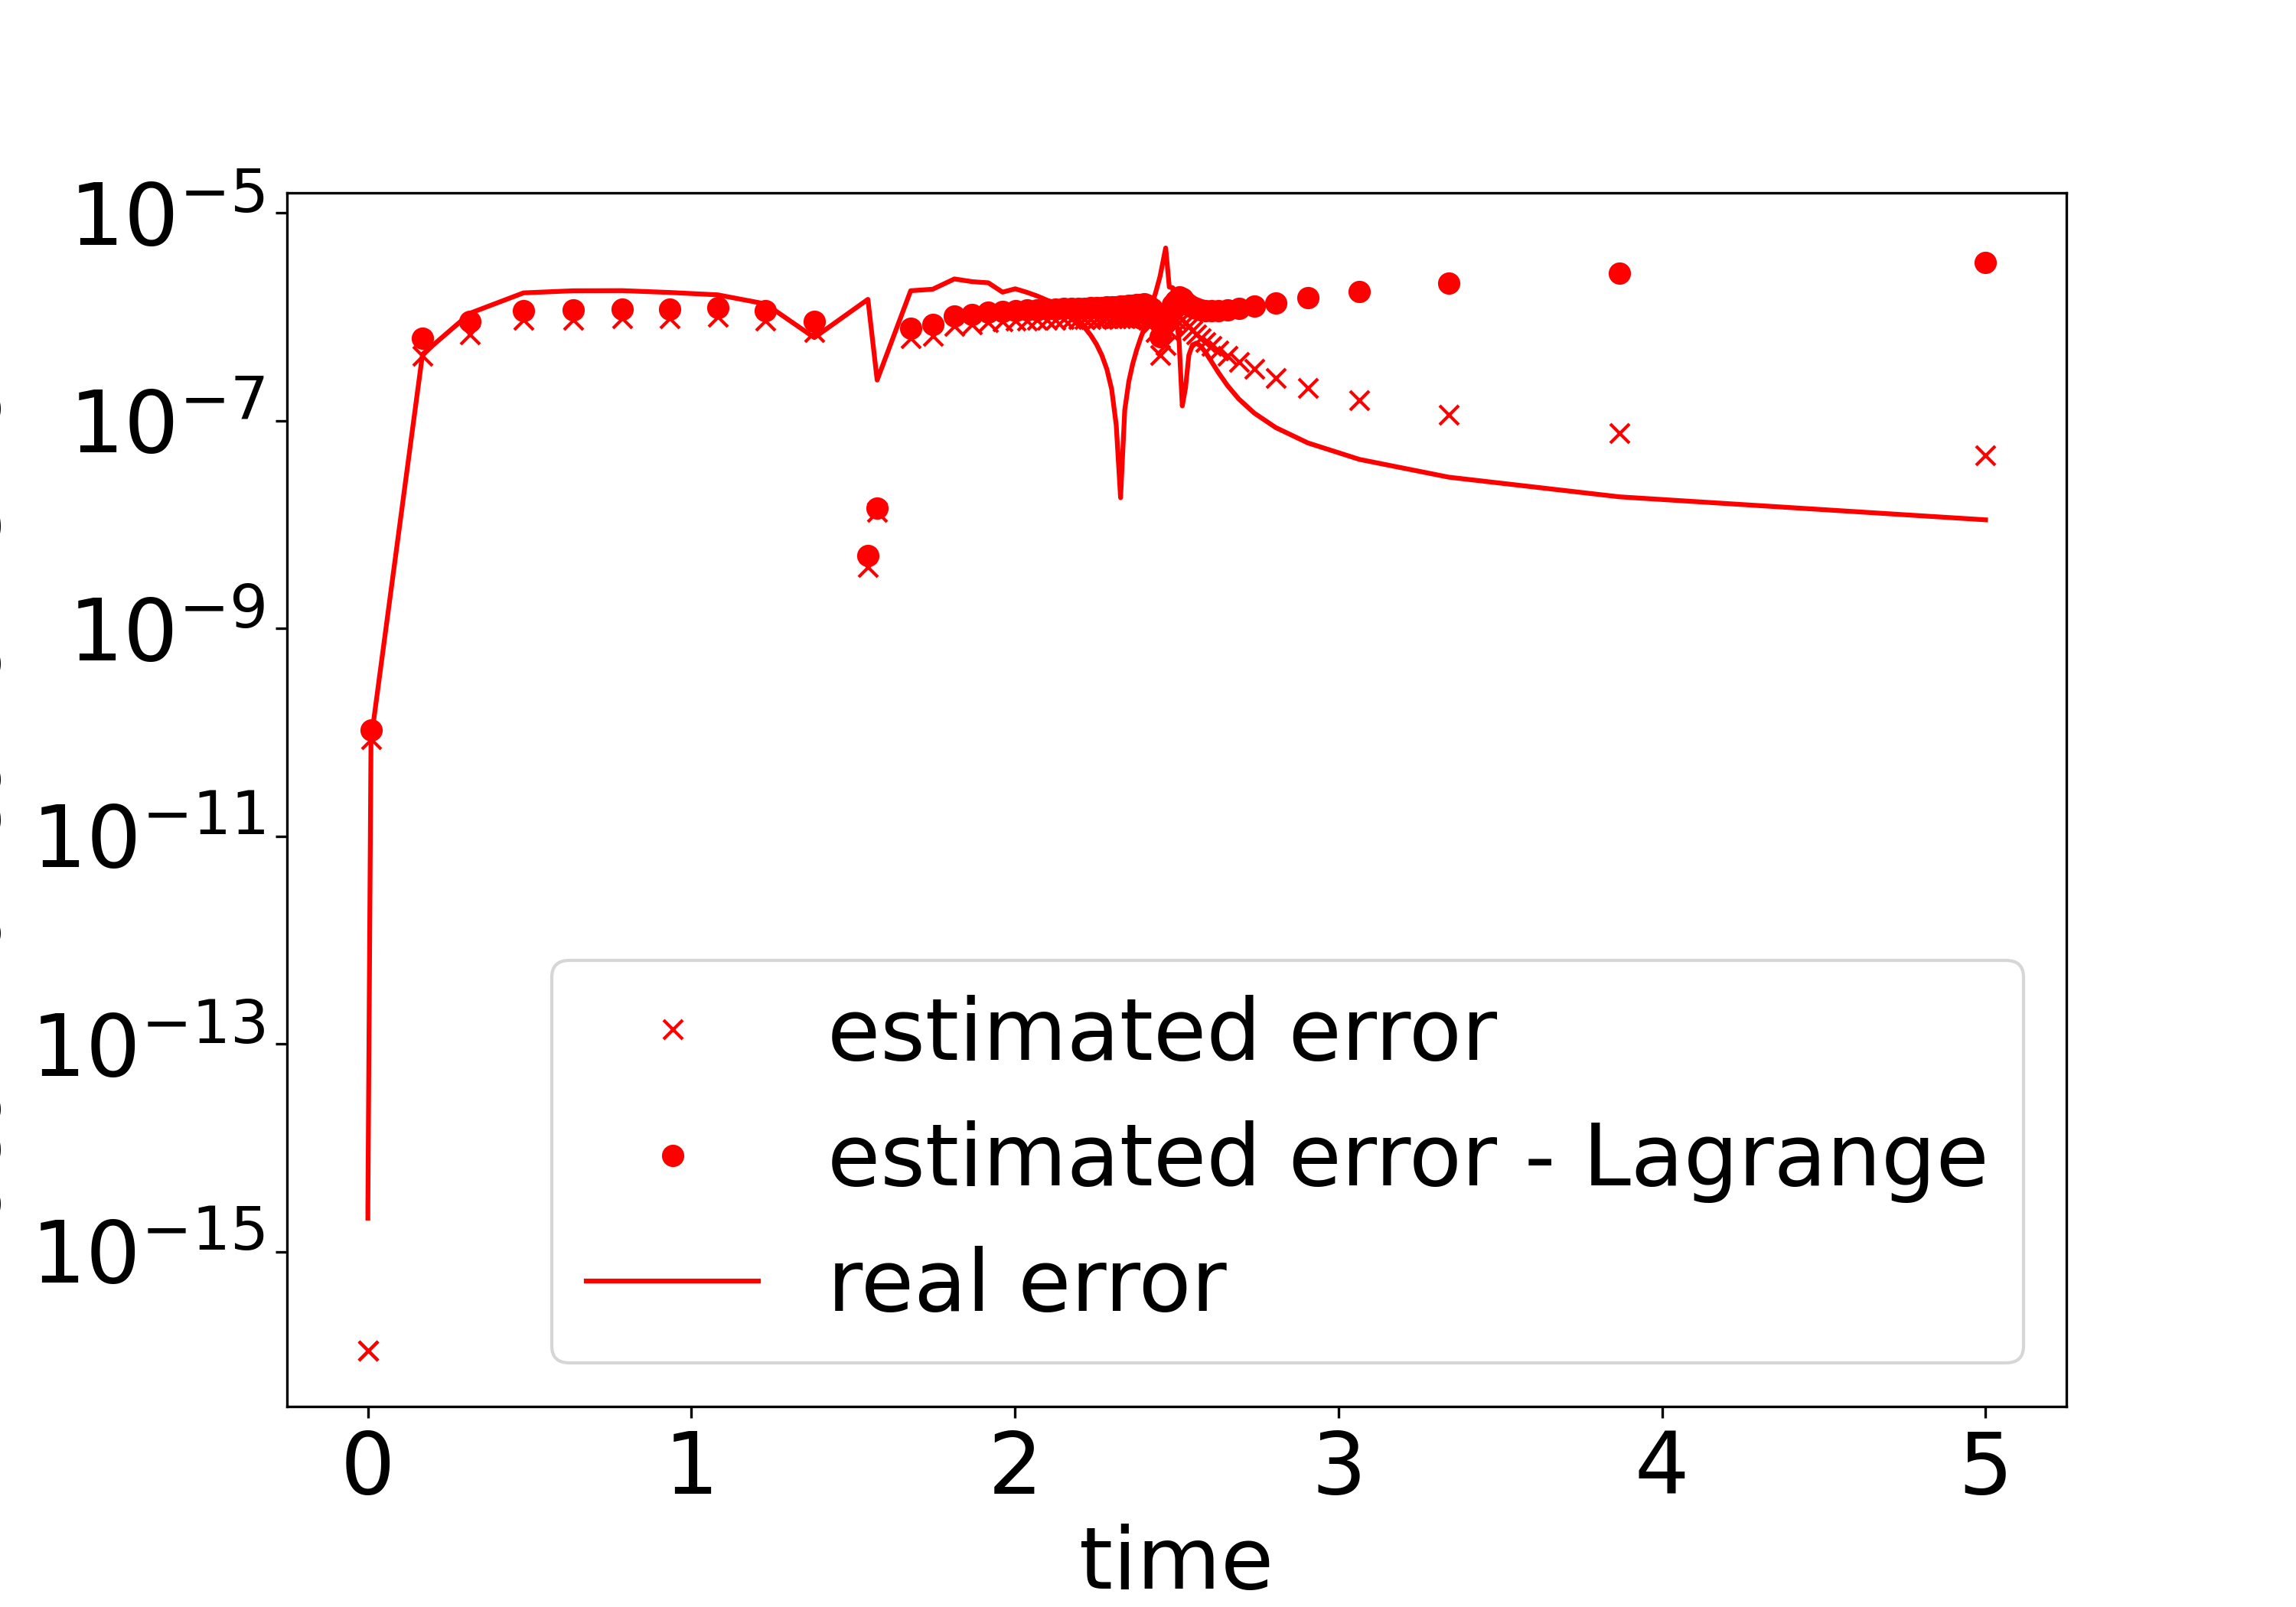
\includegraphics[width=1\textwidth]{images/errorEstimateBDF23.png}
       	\subcaption{\textbf{BDF23}} 
        \label{fig:errorEstimateEvolutionBDF23}
    \end{subfigure}
    \caption{Evolution of the local truncation error and of the error estimate for the single state problem defined in \autoref{eq:first_DAE_algeb} with the implemented numerical schemes}
    \label{fig:errorEstimateEvolutionALL}
\end{figure}

In conclusion, the implicit BDF23 method gives the best results because overall, the induced total error remains low, it allows for the highest timestep sizes and the local truncation error is generally well estimated. In contrast, the BDF12 method is restricted to much smaller timesteps which makes it unattractive for most simulations. Another negative side effect of the small timesteps is the large difference to the analytical solution since the local errors accumulate steadily. The explicit RKF45 fails if the velocity is too high, so it should not be used in such cases. However, it has a strong potential against the BDF23 method for very small velocities because it allows for larger timesteps and in the transition phase from low to high velocities because of the better estimate of the local truncation error.



\chapter{Two-Dimensional SEAS model}
In a second step we consider a trivial SEAS model with only two dimensions and square, symmetric tectonic plates.

\section{Physical Description}
\label{ssec:physicalDescriptionSEAS2D}
--- write down Poisson/elasticity equation for the domain --- \\
--- rate and state laws for the fault --- \\
describe what all variables mean and stuff...
Ageing law: 
\begin{equation}
    \dot{\psi} = g(\psi, V) = \frac{bV_0}{L}e^{\frac{f_0 - \psi}{b}} - \frac{V}{V_0}
\end{equation}
Friction law: 
\begin{equation}
    0 = \tau(U) - a\sigma_n(U) \text{arsinh}\left(\frac{V}{2V_0}e^{\frac{\psi}{a}}\right) - \eta V
\end{equation}


\section{BP1 problem}
--- read more about BP1 and find good citations --- \\
The displacement is applied orthogonal to the represented plane, thus, if the mesh is located in the X-Y plane, each element has one traction, velocity and displacement component acting in the Z direction. In this model problem, the represented tectonic plates have a symmetric layout and move in opposite direction, as one moves into the plane and the other one out of the plane. Therefore, it is enough to consider only one half of the domain, as the results in the other half will be identical, but with opposite sign. \autoref{fig:mesh_BP1_200_fault_elements} depicts the half-domain on which the solution is calculated. The fault here is located on the left side of the domain.
\begin{figure}[H]
    \centering
    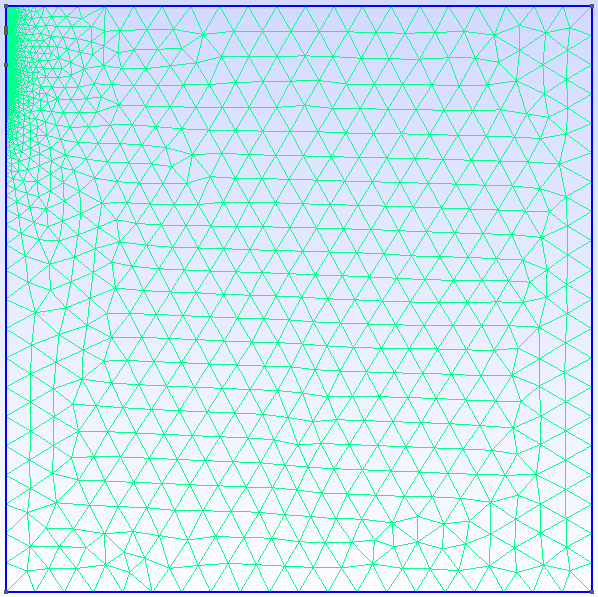
\includegraphics[width=0.4\textwidth]{images/BP1_MESH_200.png}
    \caption{Space discretization of the BP1 problem with 200 elements on the fault}
    \label{fig:mesh_BP1_200_fault_elements}
\end{figure}

In the considered example, we choose the mesh such that there are 200 elements at the fault. The lower end of the plates is pulled with a constant velocity $V_0 = 10^{-6} m\cdot s^{-1}$. 

\section{Formulation of the Discontinous Galerkin}

--- write something about DG --- \\ 


The numerical integration is achieved with the Gaussian quadrature. For that, Gauss-Legendre polynomials up to order $p$ are chosen to interpolate relevant values on each element. Dependent on the chosen order $p$, the solution has to be calculated at different points $x_i$ within the element and, associated with the correct weights to interpolate the data over the entire element, the integration is exact with respect to the interpolation polynomials. \\
--- write more about GQ --- \\

To solve the Poisson equation, it is necessary to evaluate the integral over the entire element and to handle boundary conditions and the fault, the integral over the edges of the element is needed. 


\section{First Order Differential Equation}
The problem stated in \autoref{ssec:physicalDescriptionSEAS2D} is a first order DAE, as the involving terms only depend on the unknown quantities and at most there first time derivatives:
\begin{align}
    \dot{S_i} &= V_i \label{eq:SEASDAE_dV_dt} \\
	\dot{\psi_i} &= g(\psi_i, V_i) =\frac{bV_0}{L}\left(e^{\frac{f_0-\psi_i}{b}} - \frac{V_i}{V_0}\right) \label{eq:SEAS_DAE_ageing_law} \\
	0 &= f_i(U,S,\psi,V) = \tau_i(U,S) - a\sigma_n\text{arsinh}\left(\frac{V_i}{2V_0}e^{\frac{\psi_i}{a}}\right) -\eta V_i \label{eq:SEASDAE_frictionLaw}\\
    0 &= AU - b(S) \label{eq:SEAS_DAE_AU=b}  
\end{align}
The index $i\in[0,n]$ refers to all interpolation points of the elements located on the fault, meaning that $S_i$, $V_i$ and $\psi_i$ are respectively the slip, the velocity and the value of the state variable on the fault. The matrix-vector system in \autoref{eq:SEAS_DAE_AU=b} stems from the DG formulation of the Poisson problem and needs to be solved for all nodes with index $j\in[0,N]$ in the DG domain. Usually, there are much more nodes in the full domain then purely on the fault, so $n \ll N$. The slip $S_i$ at the fault is related to the displacement $U_j$ by $\llbracket U_j \rrbracket = U_j^+ - U_j^- = -S_i$, where $j$ is the index of the fault node $i$ in the discretization of the full DG domain. The displacements $U_j^+$ and $U_j^-$ correspond to the displacements on the two sides of the fault, for the current symmetric problem, they have the same magnitude with opposite signs. Outside of the fault, the term $S$ is used to enforce boundary conditions on the domain, and typically increases with time, simulating constant tectonic movements of the plates. Nodes on the fault will first resist to this environment slip and when the forces reach a certain level, an earthquake is triggered. \\
To use implicit time solvers, a nonlinear equation has to be solved at each time step. For this purpose, Newton iterations are often used, however they require the Jacobian matrices of the right-hand side functions in (\ref{eq:SEAS_DAE_ageing_law}) and (\ref{eq:SEASDAE_dV_dt}). In general, if it is unknown, it is approximated along with the solution during the Newton iteration using for instance a Broyden iteration [cite Broyden]. However, this impairs the convergence speed of the Newton iteration compared to the analytical expression. It is especially relevant if a DAE formulation of the problem is chosen, for which an iterative solver is indispensable. An analytic expression of the Jacobian is provided for both the ODE and the DAE formulations of the problem, so that the Newton iterations can be solved efficiently when using implicit methods.
 

\subsection{Formulation as a first order ODE}
\subsubsection{Problem}
The first approach to solve the problem is to formulate the system as a classical ODE. The solution vector contains the values for the slip and for the state variable, and at each timestep, the the slip rate $V$ is calculated from \autoref{eq:SEASDAE_frictionLaw} from the state with an iterative solver.
\begin{align}
	\label{eq:ODE_formulation_SEAS}
	x &= \begin{pmatrix}
		S \\ \psi
	\end{pmatrix} & \dot{x} &= \begin{pmatrix}
								  \dot{S} \\ \dot{\psi}
							   \end{pmatrix} = \begin{pmatrix}
												   V(S,\psi) \\ g(\psi, V)
											   \end{pmatrix} = F
\end{align} 
Such a formulation allows us to use many well-known and proved numerical schemes, both implicit and explicit. 

\subsubsection{Jacobian matrix}
\label{sssec:Jacobian_ODE}
For the ODE formulation in \autoref{eq:ODE_formulation_SEAS}, it is not straightforward to calculate the Jacobian matrix because of the implicit evaluation of the slip rate within the right-hand side function. The matrix $\mathbf{J}_{\psi,S}(F)$ consists of four block matrices, which each contains the Jacobians related to the two quantities:
\begin{equation}
\label{eq:Jacobian_ODE_formulation}
\mathbf{J}_{\psi_j,S_j}\left(F_i\left(\psi,V(\psi,S)\right)\right) = \begin{pmatrix} 
\frac{\partial V_i}{\partial S_j} &
\frac{\partial V_i}{\partial \psi_j} \\ 
\frac{\partial g(\psi_i,V_i)}{\partial S_j} &
\frac{\partial g(\psi_i,V_i)}{\partial \psi_j}  \end{pmatrix}
\end{equation}
In a first step, the partial derivatives of the slip rate $V$ will be calculated. As this quantity is obtained implicitly from the friction law in \autoref{eq:SEASDAE_frictionLaw}, the implicit function theorem has to be applied. The function $f()$ is continuously differentiable and its Jacobian matrix with respect to the slip rate $\frac{\partial f}{\partial V}$ is invertible. Indeed, from the analytic expression in \autoref{eq:partial_df_dV}, it appears that the matrix is diagonal and its entries are all non-zero. All necessary conditions to apply the implicit function are fulfilled and it states that the partial derivatives of $V$ are given by the product:
\begin{align}
\frac{\partial V}{\partial S} &= -\left(\frac{\partial f}{\partial V}\right)^{-1}\frac{\partial f}{\partial S} \\ 
\frac{\partial V}{\partial \psi} &= -\left(\frac{\partial f}{\partial V}\right)^{-1}\frac{\partial f}{\partial \psi} 
\end{align}
Two of the occurring Jacobian matrices can be easily obtained from the respective derivatives of the friction law. 
\begin{equation}
\frac{\partial f_i(S,\psi,V)}{\partial \psi_j} = \left( -\frac{\sigma_n}{2V_0} \frac{Ve^{\frac{\psi_i}{a}}}{\sqrt{\frac{e^{\frac{2\psi_i}{a}}V_i^2}{4V_0^2}+1}}\right)\delta_{ij} 
\label{eq:partial_df_dpsi}
\end{equation}	
\begin{equation}
\frac{\partial f_i(S,\psi,V)}{\partial V_j} = \left( -\frac{\sigma_na}{2V_0} \frac{e^{\frac{\psi_i}{a}}}{\sqrt{\frac{e^{\frac{2\psi_i}{a}}V_i^2}{4V_0^2}+1}}-\eta\right)\delta_{ij} 
\label{eq:partial_df_dV}
\end{equation}
Since $\frac{\partial f}{\partial V}$ is a diagonal matrix, its inverse is very easy to calculate and does not require to solve a linear system of equations. The evaluation of the last missing partial derivative is more complex to obtain and will be one reason for a partial filling of the Jacobian matrix.
\begin{align}
\label{eq:partialDerivative_df_dS}
\frac{\partial f_i}{\partial S_j} = \frac{d \tau_i(U)}{d S_j} = \frac{\partial \tau_i(U)}{\partial U_k}\frac{\partial U_k}{\partial S_j} + \frac{\partial \tau_i(U)}{\partial S_j}
\end{align}
The problem shifted to calculate the partial derivative $\frac{\partial U}{\partial S}$. Since $U = A^{-1}b(S)$ and the matrix $A$ does not depend on $S$, we just need to find the derivative of $b(S)$. We get, for elements on the fault:
\begin{align}
\frac{\partial b_i(S)}{\partial S_j} &= \frac{\partial }{\partial S_j}\int_e \eta \{\{c_{mnkl}\epsilon_{kl}(w)\eta_n^e\}\}\llbracket U_m \rrbracket + \frac{\delta_e}{|e|^\beta}\llbracket U_m \rrbracket\llbracket w_m \rrbracket dx
\end{align}
As already stated earlier, we have $\llbracket U_i \rrbracket = -S_i$, therefore we can straight eliminate this term. On all other interpolation points not located on the fault, the right hand side $b$ does not depend on the fault displacement $S$ and the derivatives at these points consequently vanish. We then obtain:
\begin{equation}
\frac{\partial b_i(S)}{\partial S_j} = -\int_e 
\eta  \{\{c_{jnkl}\epsilon_{kl}(w)\eta_n^e\}\} +
\frac{\delta_e}{|e|^\beta}\llbracket w_j \rrbracket dx
\end{equation}
This expression can be calculated by plugging the unit vector $e^i$ as argument of the right-hand side vector $b$. The Jacobian term $\frac{\partial U_i}{\partial S_j}$ is therefore evaluated by applying the solver method of the Poisson problem to the unit vectors as slips. We get:
\begin{equation}
\frac{\partial U_i}{\partial S_j} = A_{ik}^{-1}b_k(e^i)
\end{equation}
The traction term $\tau(U,S)$ is calculated as $\tau = \mu \frac{\partial u}{\partial x_i}n_i$, and is numerically approximated on the nodal basis as $\tau_p = M_{rp}^{-1}e_{qr}^Tw_q(\nabla u)_{kq}n_{kq}$, where $M$ is the mass matrix of the fault basis, $e^T$ maps from fault to quadrature points, $w$ are the quadrature weights and $n$ is the normal at the quadrature points. The gradient of $u$ is approximated by $(\nabla u)_{pq} = \frac{1}{2}\left(D_{lpq}^0u_l^0 + D_{lpq}^1u_l^1\right) + c_0\left(E_{lq}^0u_l^0 - E_{lq}^1u_l^1 - f_q\right)n_{pq}$. The tensor $E$ maps from the quadrature points to the element basis and $D$ is its gradient and the superscripts $0$ and $1$ refer to the adjacent elements on opposite sides of the fault. The term $f_q$ denotes the actual slip transformed to the quadrature points. The evaluation of the derivative of the traction with respect to the displacement requires to derivate the gradient of the displacement with respect to itself. We obtain: 
\begin{align}
\frac{(\nabla u)_{pq}}{\partial u_k} &= \frac{1}{2}\left(D_{lpq}^0\frac{\partial u_l^0}{\partial u_k} + D_{lpq}^1\frac{\partial u_l^1}{\partial u_k}\right) + c_0\left(E_{lq}^0\frac{\partial u_l^0}{\partial u_k} - E_{lq}^1\frac{\partial u_l^1}{\partial u_k}\right)n_{pq} \\
&= \frac{1}{2}\left(D_{lpq}^0\delta_{lk}^0 + D_{lpq}^1\delta_{lk}^1\right) + c_0\left(E_{lq}^0\delta_{lk}^0 - E_{lq}^1\delta_{lk}^1\right)n_{pq} \\
&= \frac{1}{2}\left(D_{kpq}^0 + D_{kpq}^1\right) + c_0\left(E_{kq}^0 - E_{kq}^1\right)n_{pq} 
\end{align}
And further we get: 
\begin{equation}
\frac{\partial \tau_p}{\partial u_l} = M_{rp}^{-1}e_{qr}^Tw_q
\frac{(\nabla u)_{kq}}{\partial u_l}n_{kq}
\end{equation}
In addition, the traction needs to be derivated with respect to the current slip directly for the term $\frac{\partial \tau_i(U)}{\partial S_j}$, which is contained in the term $f_q = e_{qj}S_j$. It appears again in the gradient, so its derivative with respect to the slip is also needed. 
\begin{align}
\frac{(\nabla u)_{pq}}{\partial S_j} = -c_0 \frac{\partial f_q}{\partial S_j}n_{pq} 
= -c_0 e^T_{qk}\frac{\partial S_k}{\partial S_j}n_{pq} 
= -c_0 e^T_{qj}n_{pq} \\	
\end{align}
With this expression, we obtain: 
\begin{equation}
\frac{\partial \tau_p}{\partial S_j} = -M_{rp}^{-1}e_{qr}^Tw_qc_0e^T_{qj}n_{kq}n_{kq}
\end{equation}
This derivative term does not depend on the current slip anymore but only on the geometry of the discretization, so it can be calculated once at the beginning of the simulation. All components of the remaining partial derivative in \autoref{eq:partialDerivative_df_dS} are now available and the Jacobian matrices of the slip rate with respect to the slip and to the state variable can be calculated. \\
To express the full Jacobian matrix of the ODE in \autoref{eq:Jacobian_ODE_formulation}, the partial derivatives of the ageing law $g(\psi, V)$ are still missing. They can be expressed in term of the already known partial derivatives: 
\begin{align}
\frac{\partial g_i}{\partial S_j} &= -\frac{b}{L}\frac{\partial V}{\partial S} \\
\frac{\partial g_i}{\partial S_j} &= -\frac{V_0}{L}e^{\frac{f_0 - \psi}{b}}\delta_{ij} -
\frac{b}{L}\frac{\partial V}{\partial \psi}
\end{align}



\subsection{Formulation as a DAE}
\subsubsection{Problem}
The ODE form looks pretty and like an easy-to-tackle numerical problem, but may run into some trouble because of the implicit evaluation of the slip rate, which is treated independently of the numerical integration. Alternatively, the friction law could be solved for the slip rate together with the time-variant solution components. The solution vector is then extended by one quantity, and the evaluation of the slip rate with a separate iterative does not occur anymore.
\begin{align}
	\label{eq:DAE_formulation_SEAS}
	x &= \begin{pmatrix}
			S \\ \psi \\ V
		 \end{pmatrix} & \dot{x} &= \begin{pmatrix}
										\dot{S} \\ \dot{\psi} \\ 0
									\end{pmatrix} = \begin{pmatrix}
										V \\ g(\psi, V) \\ f(S,\psi,V)
									\end{pmatrix}
\end{align}
This system cannot be used anymore with pure explicit solvers, since no time discretization can be set up for the algebraic equation. It is however well-suited for implicit methods, which iteratively solve for the time-variant quantities $S$ and $\psi$ as well for the algebraic state $V$. A notable advantage of this formulation is that the tolerances of the numerical solver can be specified independently for $S$, $\psi$ and $V$, whereas in the ODE formulation of the problem, the error control is limited to the parameters $S$ and $\psi$. \\
The PETSc interface requires us to provide a DAE in the form
\begin{align}
	F(t, x,\dot{x}) = G(t,x) 
\end{align}
where the left-hand side function $F()$ depends on the solution vector and its time derivative whereas the right-hand side function $G()$ only depends on the solution vector. For now, we choose a fully implicit formulation of the problem, in which $G()$ vanishes. The DAE can then be expressed in the following way: 
\begin{align}
\label{eq:DAE_extended_formulation_SEAS}
	x &= \begin{pmatrix}
		S \\ \psi \\ V
	\end{pmatrix} & F(t, x,\dot{x}) &= \begin{pmatrix}
	 	V - \dot{S} \\ g(\psi, V) - \dot{\psi}  \\ f(S,\psi,V)
	\end{pmatrix} = \begin{pmatrix}
		0 \\ 0 \\ 0
	\end{pmatrix} = G(t,x)
\end{align}

Another class of solvers, the so called IMEX (implicit-explicit) solvers [cite IMEX], offer an interesting approach to numerically solve this problem, by mixing an implicit, iterative method for the algebraic states with an explicit method for the remaining simple time-dependent quantities. Technically, the function $F()$ is expected to be integrated implicitly, while the right-hand side function $G()$ is solved explicitly. In the given formulation, the right hand side is equal to 0, this means that the system has to be solved fully implicitly and the advantages of IMEX methods cannot be used here. 

\subsubsection{Jacobian matrix}
\label{sssec:Jacobian_DAE}
For the DAE formulation of the system in \autoref{eq:DAE_extended_formulation_SEAS}, another approach can be chosen to calculate the Jacobian matrix of the system. With now three different components in the solution vector, the Jacobian matrix contains the partial derivatives with respect to the slip rate in addition to the slip and to the state variable. Similarly, the function $F$ on which the Jacobian is applied is extended by the friction law. Each block $i,j$ in the structure of the Jacobian is given by:
\begin{equation}
\label{eq:Jacobian_DAE_formulation}
\mathbf{J}_{S_j,\psi_j,V_j}F_i(S,\psi,V) = 	\begin{pmatrix}
\frac{\partial V_i}{\partial S_j} & \frac{\partial V_i}{\partial \psi_j} & \frac{\partial V_i}{\partial V_j} \\
\frac{\partial g_i(\psi,V)}{\partial S_j} & \frac{\partial g_i(\psi,V)}{\partial \psi_j} & \frac{g_i(\partial \psi,V)}{\partial V_j} \\
\frac{\partial f_i(S,\psi,V)}{\partial S_j} & \frac{\partial f_i(S,\psi,V)}{\partial \psi_j} & \frac{\partial f_i(S,\psi,V)}{\partial V_j}
\end{pmatrix}
\end{equation}
In the previous section, a complicated approach had to be followed to obtain the derivative for the slip rate because of the nonlinear friction law, which was indirectly solved for each evaluation of the slip rate. Since the slip rate is now obtained directly from the solution vector $x$ and not from an iterative solver for the friction law, all its partial derivatives except with each component itself vanish. 

\begin{align}	
\frac{\partial V_i}{\partial S_j} &= 0 & \frac{\partial V_i}{\partial \psi_j} &= 0 & \frac{\partial V_i}{\partial V_j} &= \delta_{ij}
\end{align}

Similarly, the partial derivatives of the ageing law can be directly evaluated from its definition in \autoref{eq:SEAS_DAE_ageing_law}.
\begin{align}
\frac{\partial g_i(\psi,V)}{\partial S_j} &=  0 &
\frac{\partial g_i(\psi,V)}{\partial\psi_j} &= -\frac{V_0}{L}e^{\frac{f_0-\psi_i}{b}}\delta_{ij} &	
\frac{\partial g_i(\psi,V)}{\partial V_j} &= -\frac{b}{L} \delta_{ij}
\end{align}
For the friction law, the Jacobian matrices have already been calculated in \autoref{eq:partial_df_dpsi} for $\frac{\partial f(S,\psi,V)}{\partial psi}$, in \autoref{eq:partialDerivative_df_dS} for $\frac{\partial f(S,\psi,V)}{\partial S}$ and in \autoref{eq:partial_df_dV} for $\frac{\partial f(S,\psi,V)}{\partial V}$.

This formulation of the Jacobian cannot be directly used in the Newton iteration to calculate the next timestep. Typically, the Jacobian has to be adapted to represent the time-stepping scheme. For instance, the implicit Euler method results requires to solve the nonlinear equation $0 = 1/h(x_n - x_{n+1}) + F(x_{n+1})$ for the solution at the next timestep $x_{n+1}$ and the Jacobian matrix $J_N$ for the corresponding Newton iteration is constructed from $J$. 
\begin{equation}
J_N = -\frac{1}{h}I + J
\end{equation}
Here, the problem arises that the evolution over time is only defined for two components in the solution vector: the slip $S$ and the state variable $\psi$. The slip rate $V$ needs to be solved algebraically at every Newton iteration, but this component should not be included in the time-stepping scheme. The nonlinear equation to calculate a step of the implicit Euler has to be adapted to include properly the slip rate. 
\begin{align}
0 = \begin{pmatrix} \frac{1}{h}S_n     \\ \frac{1}{h}\psi_n     \\ 0 \end{pmatrix} - 
\begin{pmatrix} \frac{1}{h}S_{n+1} \\ \frac{1}{h}\psi_{n+1} \\ 0 \end{pmatrix} + 
\begin{pmatrix} V_{n+1}            \\ g(\psi_{n+1},V_{n+1}) \\ f(S_{n+1}, \psi_{n+1}, V_{n+1}) \end{pmatrix}
\end{align}
The Jacobian matrix to be used in a Newton iteration to solve this problem has to be changed accordingly.
\begin{align}
\label{eq:Jacobian_Newton_Iteration_extended_DAE}
\mathbf{J}_N = 
\begin{pmatrix} 
-\frac{1}{h}\mathbf{I} & \mathbf{0}            & \mathbf{0} \\ 
\mathbf{0}             &-\frac{1}{h}\mathbf{I} & \mathbf{0} \\ 
\mathbf{0}             & \mathbf{0}            & \mathbf{0} 
\end{pmatrix} + 
\begin{pmatrix}  
\mathbf{J}_S(S)    &  \mathbf{J}_\psi(S)    &  \mathbf{J}_V(S)    \\ 
\mathbf{J}_S(\psi) &  \mathbf{J}_\psi(\psi) &  \mathbf{J}_V(\psi) \\ 
\mathbf{J}_S(V)    &  \mathbf{J}_\psi(V)    &  \mathbf{J}_V(V)
\end{pmatrix} =
\begin{pmatrix} 
-\frac{1}{h}\mathbf{I}         &  \mathbf{0} 			            &
\mathbf{I}                     \\ 
\mathbf{0}                    & 
-\frac{1}{h}\mathbf{I} +  \frac{\partial g}{\partial \psi}       &  \frac{\partial g}{\partial V} \\ 
\frac{\partial f}{\partial S} & \frac{\partial f}{\partial \psi} &  \frac{\partial f}{\partial V} 
\end{pmatrix}
\end{align}
If other implicit numerical schemes are used than the implicit Euler, such as higher order BDF methods, $\mathbf{J}_N$ can be easily changed by multiplying the identity matrices $\mathbf{I}$ with a coefficient that depends on the chosen method. Albeit this formulation of the Jacobian matrix is perfectly valid, it is very specific to the SEAS problem and is therefore hard to implement as such within the PETSc framework. \\
To solve general implicit DAEs of the form $F(t,x,\dot{x}) = G(t,x)$, PETSc offers a convenient interface to provide the Jacobian matrices. In fact, three matrices have to be provided. The first Jacobian matrix, denoted by $\mathbf{F}_{\dot{x}}$, corresponds to the variation of the left-hand side function $F()$ with respect to the derivative of the solution vector. The second matrix $\mathbf{F}_x$ describes the variation of the same function under the actual solution vector. Finally, the third Jacobian matrix $\mathbf{G}_x$ represents the variation of the right hand side function $G()$ under the influence of $x$. In our case, the formulation is fully explicit and the right hand side function $G(t,x)$ is zero everywhere, and by extension, its Jacobian matrix $\mathbf{G}_x$ also vanishes. It remains to express the Jacobian matrix of the Newton iteration $\mathbf{J}_N$ in terms of $\mathbf{F}_x$ and $\mathbf{F}_{\dot{x}}$:
\begin{equation}
\mathbf{J}_N = \frac{dF}{dx_n} = \mathbf{F}_{\dot{x}}\frac{d\dot{x}_n}{dx_n} + \mathbf{F}_x	
\end{equation}
The term $\frac{d\dot{x}_n}{dx_n}$ is a constant scalar and depends only on the chosen time step scheme, which can be denoted by $\sigma$. For the implicit Euler method for instance, we have $\sigma = 1/h$. The Jacobian matrix $\mathbf{F}_x$ is exactly the one expressed in \autoref{eq:Jacobian_DAE_formulation} and $\mathbf{F}_x$ contains negative identity matrices at the entries for the slip $S$ and for the state variable $\psi$.
\begin{align}
\mathbf{F}_x = \begin{pmatrix} 
\mathbf{0}                     &  \mathbf{0}                       & 
\mathbf{I}                    \\ 
\mathbf{0}                     &  \frac{\partial g}{\partial \psi} & 
\frac{\partial g}{\partial V} \\ 
\frac{\partial f}{\partial S}  &  \frac{\partial f}{\partial \psi} &  
\frac{\partial f}{\partial V} 
\end{pmatrix} &&&
\mathbf{F}_{\dot{x}} = \begin{pmatrix} 
-\mathbf{I}  &  \mathbf{0}  & \mathbf{0} \\ 
\mathbf{0}  & -\mathbf{I}  & \mathbf{0} \\ 
\mathbf{0}  &  \mathbf{0}  & \mathbf{0}
\end{pmatrix}
\end{align}
With this too matrices, the Jacobian matrix for the Newton iteration of the implicit Euler method is exactly the same as calculated in \autoref{eq:Jacobian_Newton_Iteration_extended_DAE}.



\subsection{Compact formulation as a DAE}
\subsubsection{Problem}
It is important to remember that the slip rate is the time derivative of the slip, so the variables $\dot{S}$ and $V$ are equal and can be interchanged in the problem formulation. As such, the friction law can be solved directly for $\dot{S}$ and the term $V$ is not required anymore. The solution vector then remains with the components of the slip $S$ and of the state variable $\psi$, as previously in the ODE formulation.
 \begin{align}
	\label{eq:DAE_compact_formulation_SEAS}
	x &= \begin{pmatrix}
			S \\ \psi
	     \end{pmatrix} & F(t, x,\dot{x}) &= \begin{pmatrix}
												f(S,\psi,V) \\ g(\psi, V) - \dot{\psi}
											\end{pmatrix} = \begin{pmatrix}
																0 \\ 0
															\end{pmatrix} = G(t,x)
\end{align}
As in the developed DAE formulation, the friction law is solved along with time-variant quantities $S$ and $\psi$. It therefore requires an iterative solver method from an implicit time solver and it can be used only with an implicit integrator. \\

\subsubsection{Jacobian matrix}
The compact DAE formulation of the problem in \autoref{eq:DAE_compact_formulation_SEAS} needs again to be solved fully implicitly and involves again the three Jacobian matrices, $\mathbf{F}_{\dot{x}}$, $\mathbf{F}_x$ and $\mathbf{G}_x$, where the last one also vanishes because the right-hand side function is zero. The block matrices that appear in this formulation are calculated in exactly the same way as previously but are arranged in a different manner.
\begin{align}
	\label{eq:Jacobian_compact_DAE}
	\mathbf{F}_{\dot{x}}&=  \begin{pmatrix}
								\pdv{f}{V} &  \mathbf{0} \\
							    \pdv{g}{V} & -\mathbf{I}
							\end{pmatrix} & 
	\mathbf{F}_x        &=  \begin{pmatrix}
								\pdv{f}{S} & \pdv{f}{\psi} \\
								\mathbf{0} & \pdv{g}{\psi}
							\end{pmatrix} & 
	\mathbf{G}_x        &=  \begin{pmatrix}
								\mathbf{0} & \mathbf{0} \\
							    \mathbf{0} & \mathbf{0}
							\end{pmatrix}
\end{align}

\subsection{Verification of the Jacobian matrices}
All Jacobian matrices defined in this section have been checked for accuracy. For that, a second order central finite difference approximation \cite[p. 184]{introductionPartialDiffEquations} is used to approximate each term of the Jacobian. 
\begin{equation}
	\mathbf{J}_{ij} = \pdv{F_i}{x_j} \approx \frac{F_i(x + he_j) - F_i(x - he_j)}{2h}
\end{equation}
The function $F$ has to be evaluated $2n$ times with the current solution vector $x$ and a variation $h$ applied in positive and negative direction to each component of $x$ respectively. For this, the function to evaluate the right-hand side of the ODE or respectively the left-hand side for the DAEs is called. For an appropriate choice of $h$, not too large to be accurate and not too small to avoid truncation errors, the relative error between the analytic expression of the Jacobian and its approximation is inferior to $10^{-5}$ in all components and therefore, the expressions for the Jacobian matrices can be considered to be exact.

\subsection{Practical limitations of the Jacobian matrices}
The main advantage of implicit methods over explicit methods is to allow larger time steps without loss in accuracy. The program execution is therewith expected to be accelerated. The proposed calculation of the Jacobian matrix and its application in Newton iterations comes along with some drawbacks with respect to the required calculation effort. \\
As described in \autoref{sssec:Jacobian_ODE}, the computation of the Jacobian matrix can be split up in one constant part $\frac{\partial \tau_p}{\partial S_l}$ that has to be evaluated once at the beginning of the simulation and only depends on the domain geometry and in one variable part, that needs to be updated after each evaluation of the solution vector $x_n$. The initialization can be quite computationally expensive, at it requires, for each column of $\frac{\partial \tau_p}{\partial S_l}$, to solve the Discontinuous Galerkin system for the entire domain with the corresponding unit vector as right-hand side vector. Each calculation of this linear system is approximately as expensive as performing one time iteration with an explicit solver, since solving the same linear system is the most expensive operation of a time iteration. For large domains with several hundreds or thousands of fault elements, which each contains a couple of fault nodes, this initialization operation takes a considerable amount of time. In comparison with an explicit scheme, a potential implicit method starts the race for the fastest solver with a penalty of about $n$ explicit time iterations, where $n$ is the total number of nodes on the fault. The advantages of implicit methods will therefore only pay off after a high number of iterations and make such methods of interest only if the simulated time frame is very long. \\
Another potential drawback of the Newton method is that a linear system of size $n$ needs to be solved at each iteration step. This might still sound much less than solving for the displacement on the whole DG-domain of size $N$ as it is required to evaluate the right-hand side of the ODE at each iteration too. However, the DG system has a constant matrix $A$ whose LU-decomposition can be calculated once at the beginning of the simulation and each evaluation of the right-hand side only requires a backward substitution of complexity $\mathcal{O}\left(N^2\right)$. For the Jacobi matrix, such a pre.processing is not available since it changes along with the solution vector. Every calculation to solve the linear system in the Newton iteration is achieved with a complexity of the order $\mathcal{O}\left(n^3\right)$. In particular in large domains with many fault nodes the solver with cubic complexity may involve a substantially higher execution time than the one with quadratic complexity. Notwithstanding, for such large domains, the question has to be asked whether a direct solver is still appropriate or whether iterative solvers yield acceptable results. Such considerations are however beyond the scope of this thesis.

\section{Second Order Differential Equation}
So far, the original problem in \autoref{ssec:physicalDescriptionSEAS2D} has been formulated as a first order ODE in \autoref{eq:ODE_formulation_SEAS}, in which the friction law is solved implicitly within each evaluation of the right-hand side, such that explicit time integrators can be used. The solution vector has a compact size and only includes the slip $S$ and the state variable $\psi$. Alternatively, the problem can be directly formulated as a DAE, where the solution vector is extended by the slip rate $V$, such that it can be solved through the friction law iteratively together with the time quantities $S$ and $\psi$. A compact form of the DAE has also been formulated, where the derivative slip rate is directly used in the friction law instead of introducing a new variable $V$. \\
The original motivation was to define an extended ODE formulation as counterpart to the extended DAE form, such that the solution vector contains an additional component for the slip rate $V$. To achieve this goal, it is necessary to find a function $h(t,S,\psi,V)$ which describes the change in time of the slip rate $\frac{dV}{dt}$. Since $V$ itself is the time derivative of the slip, this function $h()$ corresponds to the second time derivative of the slip, or the slip acceleration. The new ODE formulation is: 
\begin{align}
&&	 x      =& \begin{pmatrix}	S                     \\ \psi           \end{pmatrix}      &
	 		   \begin{pmatrix}	\ddot{S}              \\ \dot{\psi}     \end{pmatrix}
			=& \begin{pmatrix}	h(t,S,\psi,\dot{S})   \\ g(\psi, V)     \end{pmatrix}
			 	 		 \\ &\Leftrightarrow&	 		  		 
	 x      =& \begin{pmatrix}	S       \\ \psi       \\ V	            \end{pmatrix}      &
   	\dot{x}  = \begin{pmatrix}	\dot{S} \\ \dot{\psi} \\ \dot{V}        \end{pmatrix}
	 		=& \begin{pmatrix}	 V      \\ g(\psi, V) \\ h(t,S,\psi,V)  \end{pmatrix}
	 		 = F	
	\label{eq:2nd_order_ODE_formulation}
\end{align}
Here, the friction law does not appear in the right-hand side anymore and is implicitly included in the function $h()$. Unlike the previous ODE formulation, it does not require anymore to solve the friction law implicitly at every time step for the slip rate $V$ (or any other quantity), therefore, the new formulation is in some sense a "true" ODE and not a hidden DAE anymore. Another very beneficial advantage is, that if the boundary conditions of the DG domain are linear in time, it does not require to solve the DG system at every time step anymore, which is the main performance bottleneck after initialization in the first order formulations. 

\subsection{Derivation of the second order ODE}
This section will focus on the derivation of the right-hand side function $h(t,S,\psi,V)$, which is necessary to formulate the second order ODE. Starting point is the expression for the friction law in \autoref{eq:SEASDAE_frictionLaw}. At any time in the simulation, this algebraic equation always evaluates to zero, and therefore, its time derivative is also equal to 0. With the help of the formula of total derivatives, we obtain following expansions: 
\begin{align}
	0 = \dv{f}{t} &= \pdv{f}{t} + \pdv{f}{S}\dv{S}{t} + \pdv{f}{\psi}\dv{\psi}{t} +  \pdv{f}{V}\dv{V}{t} \\
					  &= \pdv{f}{t} + \pdv{f}{S}V + \pdv{f}{\psi}g(\psi,V) + \pdv{f}{V}h(t,S,\psi,V)
\end{align}
The partial derivatives of $f$ that occur are calculated in the same way as for the Jacobian matrices of the first order formulations. The terms $\pdv{f}{\psi}$ and $\pdv{f}{V}$ are diagonal matrices with the entries stated in \autoref{eq:partial_df_dpsi} and \autoref{eq:partial_df_dV} and the term $\pdv{f}{S}$ is a constant, full matrix which depends on the geometry of the domain and is derived in \autoref{eq:partialDerivative_df_dS}. None of these terms depends on the slip $S$ anymore, so $h()$ can be calculated independently from $S$. After some transformations, it can be expressed as: 
\begin{equation}
	\label{eq:2nd_order_ODE_formulation_sum_of_Jacobians}
	h(t,\psi,V) = -\left(\pdv{f}{V}\right)^{-1}\left(\pdv{f}{t} + \pdv{f}{S}V + \pdv{f}{\psi}g(\psi,V)\right)
\end{equation}
It can be noted that this expression is very similar to the Jacobian matrix of the first order ODE formulation. If $x=(S,\psi)^T$ stands for its solution vector and $\mathbf{J}_{S}$ denotes the first row of block matrices of its Jacobian matrix in \autoref{eq:Jacobian_ODE_formulation}, an alternative definition of $h()$ could be: 
\begin{equation}
	h(t,\psi,V) = \mathbf{J}_{S}\dv{x}{t} -\left(\pdv{f}{V}\right)^{-1}\pdv{f}{t}
\end{equation}
The last missing term is the partial derivative of the friction law $f$ with respect to the time variable $t$. In its definition, the only component that directly depends on time is the traction $\tau$ through the boundary conditions of the DG domain. Typically, at boundary nodes which are not on the seismic fault, the slip $S_b$ there is prescribed and evolves with time to represent the natural movement of the tectonic plate. For a constant environment slip rate $V_p$, we calculate $S_b=V_pt$ for the general case or $S_b=V_p/2\;t$ if the domain is symmetric. The boundary slip is linear in time, so its first derivative $\dot{S}_b$ will be constant. In the DG formulation, boundary conditions are included in the term $f_q$ of \autoref{eq:???}, and are added to the traction $\tau$ on the fault only after linear transformations. To obtain $\pdv{\tau}{t}$ on the fault, it is then sufficient to solve the Poisson problem with only $\dot{S}_b$. Since this term is constant, $\pdv{f}{t}$ is also constant it is enough to solve the Poisson problem once at the beginning of the simulation and then, at each evaluation of the right-hand side of the ODE, use the same term $\pdv{f}{t}$. To reuse existent code structures, $\pdv{\tau}{t}$ can be pre-calculated with the DG solver for $\tau$ using a slip of 0 everywhere on the fault and by evaluating the boundary condition at the time $t=1$. \\
In comparison with the first order ODE formulation, the new second order formulation needs a considerable initialization phase, but evaluates the right-hand side of the ODE much faster. In addition of the LU-decomposition of the DG matrix $A$, the initialization of the Jacobian $\pdv{f}{S}$ needs to solve the Poisson problem on the DG domain of size $N$ once per fault node, so in total $n$ times. Moreover, the problem needs to be solved once to calculate the initial condition of $V$ from the initial $S$ and $\psi$ and once to initialize the time derivative of the friction law $\pdv{f}{t}$. At each evaluation of the right-hand side of the first order ODE, the DG system needs to be solved with its LU-decomposition in $\mathcal{O}\left(N^2\right)$ and the remaining components of the vector set up in $\mathcal{O}\left(n^2\right)$ because of the matrix-vector product in $\tau$, so the total complexity is $\mathcal{O}\left(n^2+N^2\right)$. In contrast, the second order formulation only needs matrix-vector multiplications on the fault node, so its total complexity per evaluation is reduced to $\mathcal{O}\left(n^2\right)$. Since $n\ll N$, it is expected that the new formulation performs much better for long simulation times. \\
However, if the boundary conditions are not linear in time, their derivation is not constant in time anymore and needs to be evaluated at every time step, and therefore the solution of the Poisson problem is needed again at every time step. The complexity increases back to $\mathcal{O}\left(n^2+N^2\right)$ and the main advantage of the second order formulation is lost. For now, we do not consider this case and always assume that the boundary conditions are linear in time.  \\
\autoref{fig:timeEvolution_2ndOrderODE_vs_1stOrderODE} shows the maximum slip rate that occurs throughout the simulation time for both ODE formulations. Both curves overlap well, at least up to 1000 years of simulation time, so it proves that the new approach leads to the same results. This graph also indicates at which times earthquakes happen: after two initial earthquakes, a regular pattern of three close earthquakes alternates with one singular earthquake every 90 years approximately.
\begin{figure}[H]
	\centering
	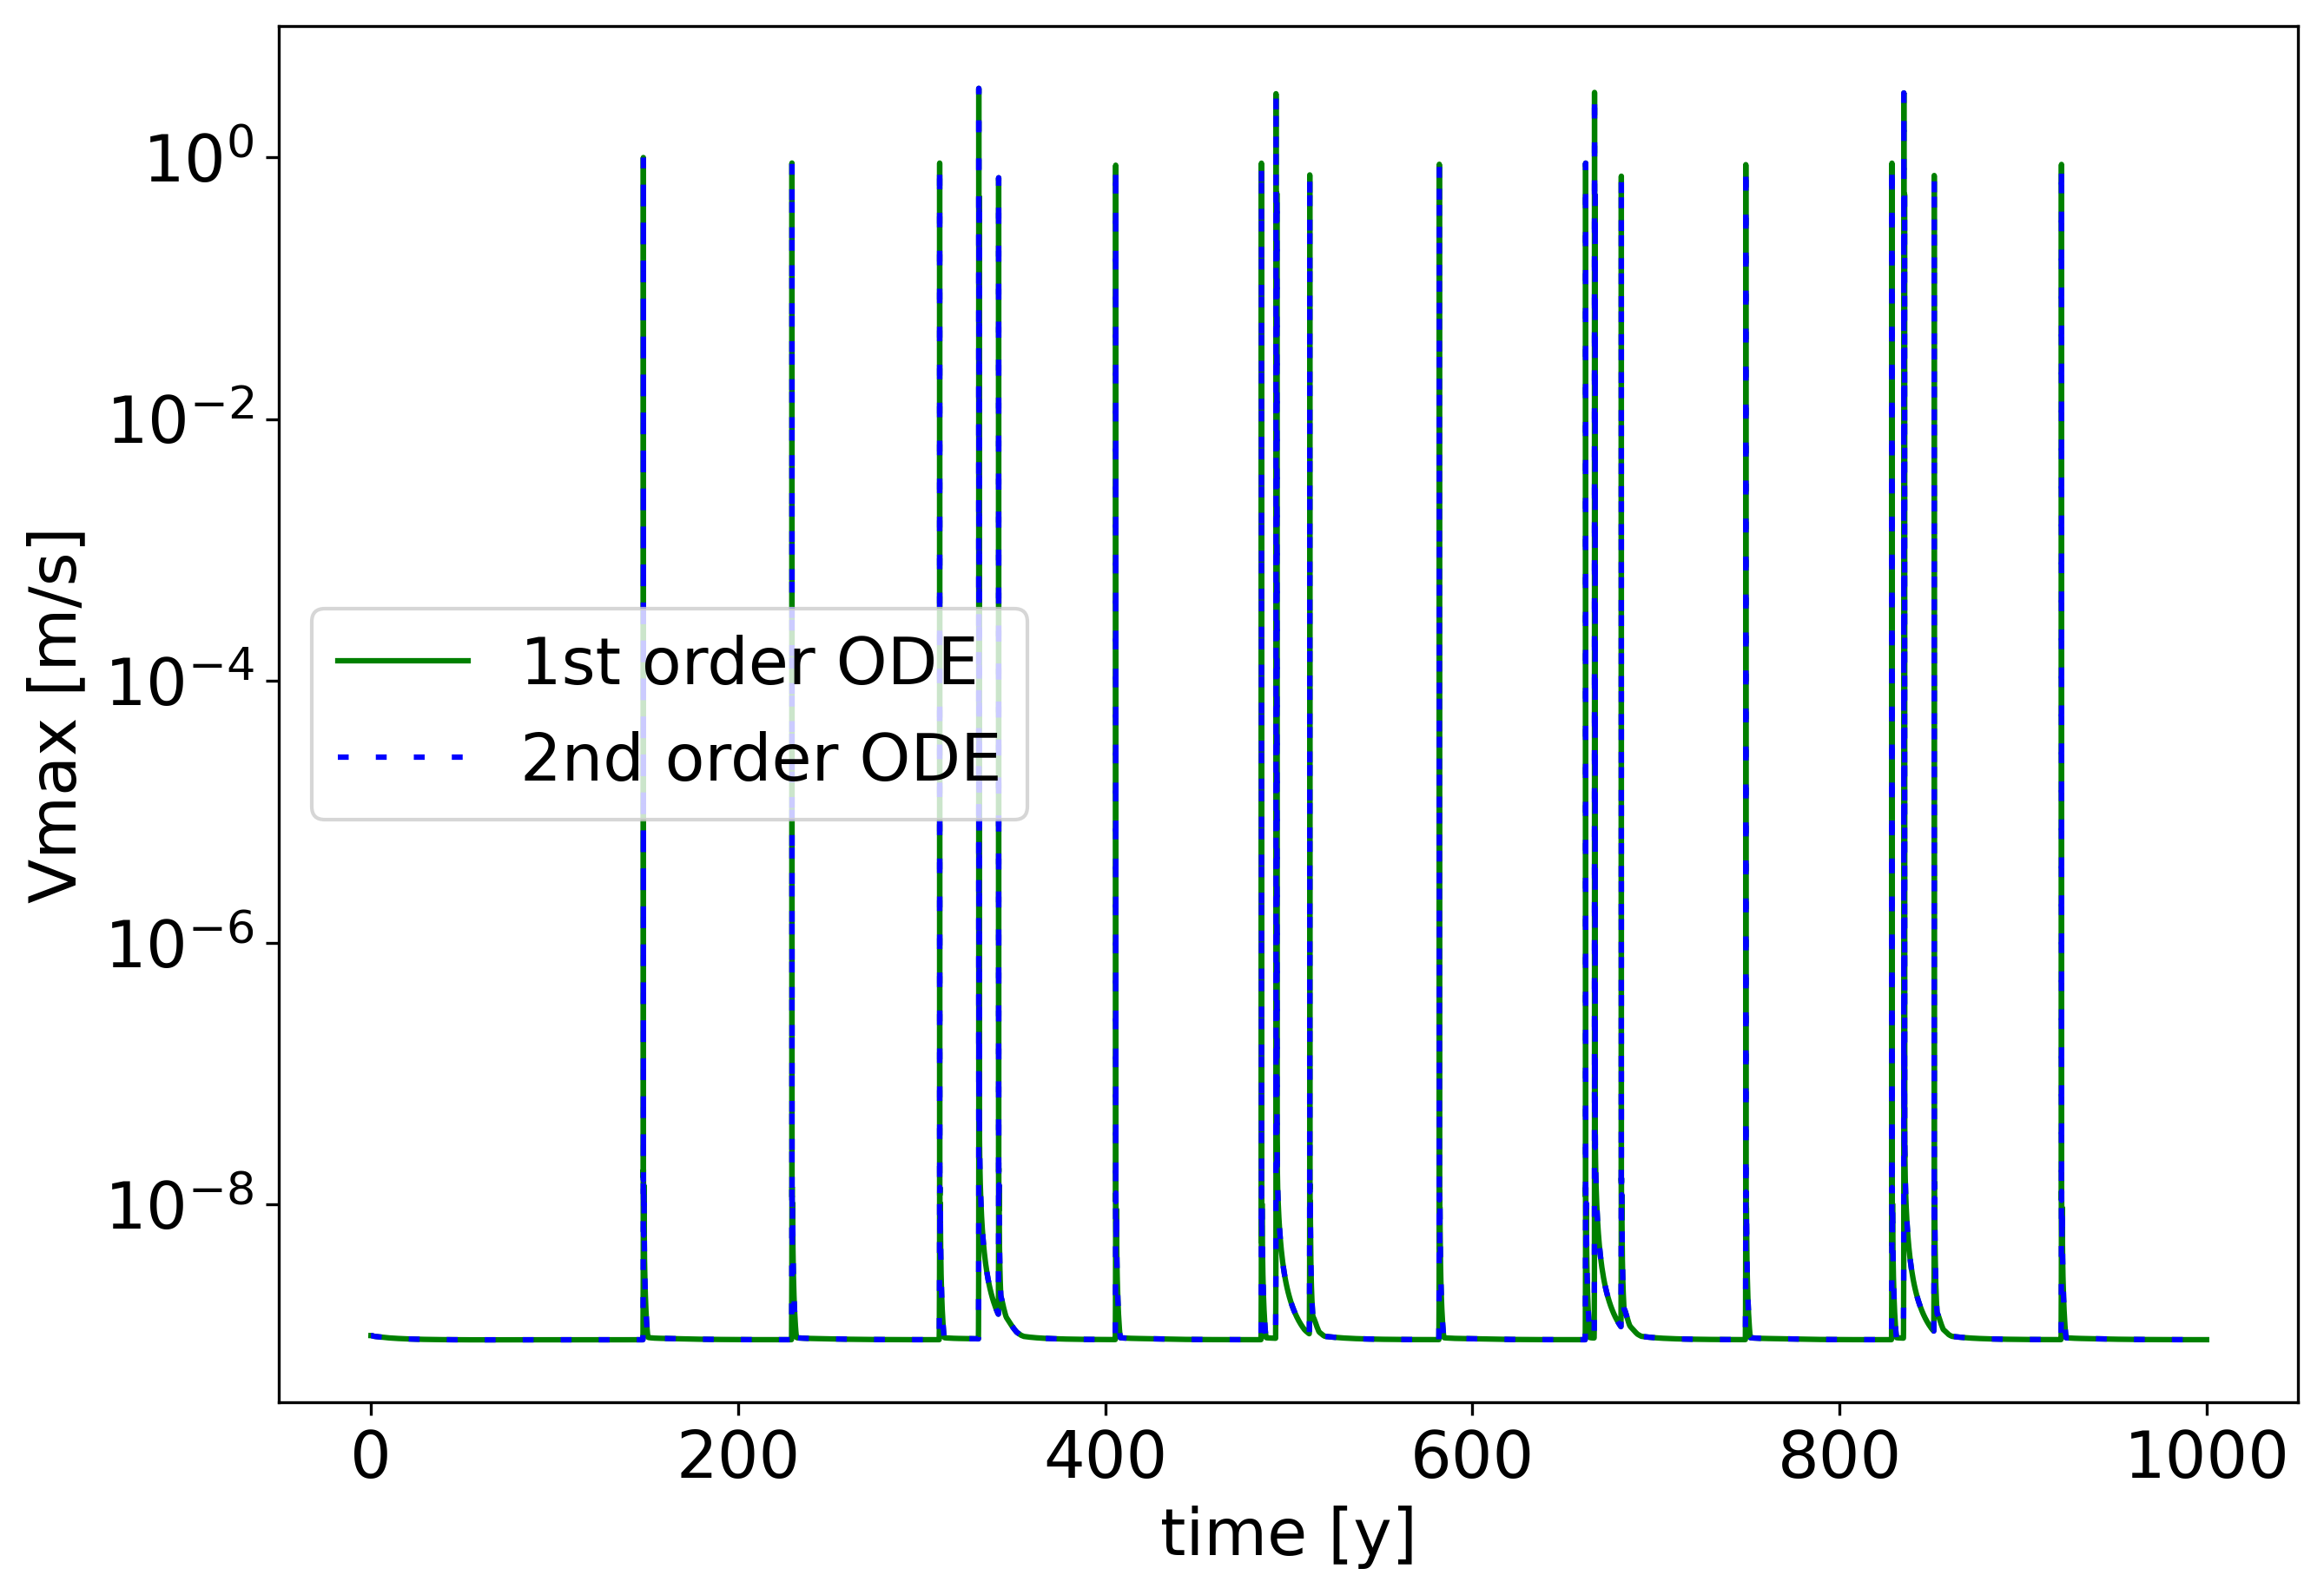
\includegraphics[width=0.45\textwidth]{images/TANDEMtimeEvolutionVExtendedODE1stvs2ndOrder.png}
	\caption{Maximum slip rate in the 1st and 2nd order formulations on a domain with 5 fault elements for 1000 years} 
	\label{fig:timeEvolution_2ndOrderODE_vs_1stOrderODE}
\end{figure}

\subsection{Derivation of the analytic Jacobian}
The Jacobian of the second order ODE formulation in \autoref{eq:2nd_order_ODE_formulation} has components in the slip $S$, the state variable $\psi$ and in the slip rate $V$. The block structure is given by:
\begin{equation}
\label{eq:Jacobian_2nd_order_ODE_formulation}
	\mathbf{J}_{S_j,\psi_j,V_j}F_i(S,\psi,V) = 	\begin{pmatrix}
	\pdv{V_i}{S_j} 				& \pdv{V_i}{\psi_j}	 			& \pdv{V_i}{V_j} \\
	\pdv{g_i(\psi,V)}{S_j} 		& \pdv{g_i(\psi,V)}{\psi_j}	 	& \pdv{g_i(\psi,V)}{V_j} \\
	\pdv{h_i(t,\psi,V)}{S_j} 	& \pdv{h_i(t,\psi,V)}{\psi_j} 	& \pdv{h_i(t,\psi,V)}{V_j}
\end{pmatrix}
\end{equation}
It can be directly seen that none of the terms $V$, $g$ and $h$ depend on the slip $S$, therefore all entries in the first column of block matrices evaluate to 0. A direct consequence is the singularity of the Jacobian matrix, which makes it unsuitable for the Newton iteration. Under consideration of all 0-entries, the matrix takes the form, where $\mathbf{K}$ is invertible with a partial diagonal structure:
\begin{equation}
\label{eq:Jacobian_2nd_order_ODE_formulation_with_zeros}
\mathbf{J}_{S_j,\psi_j,V_j}F_i(S,\psi,V) = 	\begin{pmatrix}
\mathbf{0} 												& \begin{matrix}\mathbf{0} & \mathbf{I} \end{matrix} \\
\;\,\begin{matrix}\mathbf{0} \\ \mathbf{0} \end{matrix} & \mathbf{K} 	\\
\end{pmatrix}
\end{equation}

To cope with this issue, recall that $g$ and $h$ do not depend on $S$, it is thus possible to apply the Newton iteration only on $\psi$ and $V$ with the reduced Jacobian $\mathbf{K}$. Once the slip rate $V^{(n+1)}$ is known for the next timestep, the implicit scheme can be directly applied to $S$ without the need to solve a nonlinear system of equations. Indeed, the value of the right-hand side of the ODE at the next timestep for $\dot{S^{(n+1)}} = V^{(n+1)}$ is directly available and can be plugged in the BDF scheme. If $S^{(n-i)}$ are the solutions at the $i$ previous timesteps, $\alpha_{n-i}$ the time adaptive BDF coefficients at these steps and $\sigma$ the current shift, the new slip rate $S^{(n+1)}$ can be calculated as: 
\begin{equation}
	\label{eq:update_S_2ndOrderODE}
	S^{(n+1)} = \frac{1}{\sigma}\left(V^{(n+1)} - \sum_{i=0}^{k}\alpha_{n-i}S^{(n-i)}\right)
\end{equation}

For the remaining unknown Jacobian $\mathbf{K}$, the entries in the first line are identical to the partial derivatives $\pdv{g}{\psi}$ and $\pdv{g}{V}$ \autoref{eq:Jacobian_DAE_formulation} and are trivial to compute. The entries in the second line are more challenging to obtain as they describe the variation of the product and sum of other Jacobian matrices. \\

We start from the expression for $h$ in \autoref{eq:2nd_order_ODE_formulation_sum_of_Jacobians} and introduce the new variables $C = \pdv{f}{t}$, a constant vector from the partial time derivative, $\mathbf{A} = \pdv{f}{S}$, a constant and dense matrix from the DG discretization defined in \autoref{eq:partialDerivative_df_dS}, and $\xi(\psi,V) = \left(\pdv{f}{V}\right)^{-1}$ and $\zeta(\psi,V) = \pdv{f}{\psi}$, two diagonal matrices which depend on the state variable and the slip rate. With these new variables, the components of $h$ can be expressed as:
\begin{equation}
	h_i = -\xi_{ii}\left(C_i + \mathbf{A}_{ik}V_k + \zeta_{ii}g_i\right)
\end{equation}
The first partial derivative $\pdv{h_i}{S_j}$ can be directly evaluated to 0 since none of the terms depends on the slip $S$. Next, the derivative with respect to the slip rate is already more complex:
\begin{align}
	\pdv{h_i}{\psi_j} &= -\left[\pdv{\xi_{ii}}{\psi_j}\left(C_i + \mathbf{A}_{ik}V_k + \zeta_{ii}g_i\right) + \xi_{ii}\left(\pdv{\zeta_{ii}}{\psi_j}g_i + \zeta_{ii}\pdv{g_i}{\psi_j}\right)\right]\delta_{ij}
\end{align}
The derivatives of $\xi$ and $\zeta$ can be directly computed from Equations \ref{eq:partial_df_dpsi} and \ref{eq:partial_df_dV}:

\begin{align}
	\pdv{\xi_{ii}}{\psi_j} &= \frac{2V_0\sigma_n e^{\frac{\psi_i}{a}}}{\sqrt{\frac{e^{\frac{2\psi_i}{a}}V_i^2}{4V_0^2}+1}\left(2V_0\eta\sqrt{\frac{e^{\frac{2\psi_i}{a}}V_i^2}{4V_0^2}+1}+a\sigma_n e^{\frac{\psi_i}{a}}\right)^2}\delta_{ij} \\
	\pdv{\zeta_{ii}}{\psi_j} &= -\frac{\sigma_nV_ie^{\frac{\psi_i}{a}}}{2aV_0\left(\frac{e^{\frac{2\psi_i}{a}}V^2}{4V_0^2}+1\right)^{\frac{3}{2}}}\delta_{ij}
\end{align}

The last derivative with respect to the slip rate $V$ is not a diagonal matrix anymore:
\begin{align}
	\pdv{h_i}{V_j} &= -\left[\pdv{\xi_{ii}}{V_j}\left(C_i + \mathbf{A}_{ik}V_k + \zeta_{ii}g_i\right)\delta_{ij} + \xi_{ii}\left(\mathbf{A}_{ij} + \pdv{\zeta_{ii}}{V_j}g_i\delta_{ij} + \zeta_{ii}\pdv{g_i}{V_j}\delta_{ij}\right)\right]
\end{align}
Again, the unknown derivatives can be calculated:
\begin{align}
	\pdv{\xi_{ii}}{V_j} &= -\frac{a\sigma_n V_ie^{\frac{3\psi_i}{a}}}{2V_0\sqrt{\frac{e^{\frac{2\psi_i}{a}}V_i^2}{4V_0^2}+1}\left(2V_0\eta\sqrt{\frac{e^{\frac{2\psi_i}{a}}V_i^2}{4V_0^2}+1}+a\sigma_n e^{\frac{\psi_i}{a}}\right)^2}\delta_{ij} \\
	\pdv{\zeta_{ii}}{V_j} &= -\frac{\sigma_n e^{\frac{\psi_i}{a}}}{2V_0\left(\frac{e^{\frac{2\psi_i}{a}}V_i^2}{4V_0^2}+1\right)^{\frac{3}{2}}}\delta_{ij}
\end{align}
By now, all components to set up the Jacobian matrix in \autoref{eq:Jacobian_2nd_order_ODE_formulation} are provided and the formulation is ready to be used with implicit methods. \\
In the implementation, the singularity is handled slightly differently: solving the Newton iteration with the matrix $\mathbf{K}$ in \autoref{eq:Jacobian_2nd_order_ODE_formulation_with_zeros} would require to copy the entries for $V$ and $\psi$ from the solution vector to another vector whose size matches the dimensions of $\mathbf{K}$. Instead, $\mathbf{K}$ is extended with ones on the diagonal elements related to the $S$, and in each Newton step, just before solving the linear system, the corresponding entries in the right-hand side vector are set to zero. As such, the change in $S$ always vanishes and the convergence of the Newton iteration is not altered. After a successful termination, the entries for $S$ are updated as described in \autoref{eq:update_S_2ndOrderODE}.

\section{Numerical Aspects and Implementation Details}
So far, 4 different methods have been proposed, which can be solved explicitly or implicitly. An overview of the available is given in \autoref{tab:availableMethods}, which in addition states the length of the solution vector. Methods with a size $2n$ contain the slip $S$ and the state variable $\psi$ in the solution vector, and methods with $3n$ contain in addition the slip rate $V$.
\begin{table}[H]
	\centering 
	\begin{tabular}{ | c | c c | c |}
		\hline	
						& explicit	& implicit 	& Vector length\\ \hline
		1st order ODE 	& yes 		& yes 		& 2$n$\\  
		extended DAE  	& no 		& yes 		& 3$n$\\
		compact DAE  	& no 		& yes 		& 2$n$\\
		2nd order ODE  	& yes 		& yes 		& 3$n$\\
		\hline
	\end{tabular}
	\caption{Overview of the available methods}
	\label{tab:availableMethods}
\end{table}
This section provides more details about the necessary components to solve each of these methods numerically. The focus is first on adaptive time integration methods followed by a discussion about the proper definition of tolerances. Next, the Newton iteration and its convergence properties is described to solve the nonlinear systems which arise in the implicit problem formulations. Finally, the data layout is described along with a quick estimate of the memory requirements for each problem formulation. In addition, the section exposes the peculiarities and possible limitations of the respective methods.

\subsection{Time integration}
The PETSc environment is used to handle most of the time integration. Among all available integrator, the new code is only compatible with Runge-Kutta methods for explicit formulations and BDF methods for implicit formulations. \\
For the explicit methods, the 2nd order Bogacki-Shampine scheme with a 3rd order error estimate and the 4th order Dormand-Prince scheme with a 5th order error estimate will be compared later in the results section. Their respective Butcher tableaus are given in /:TODO////---APPENDIX-----////. \\
For now, only the basic PETSc timestep adapter is used. The next timestep size is calculated in function of the estimation of the local truncation error $\epsilon$ and of the order of the estimate $\bar{k}$. In general, $\bar{k}=k+1$, where $k$ is the order of the numerical scheme. 
\begin{equation}
	h_{n+1} = C\epsilon^{-1/\bar{k}}h_n
\end{equation}
The safety factor $C$ is set to 0.9, and the scaling from one timestep to another is restricted to values between 0.1 and 10. In the native PETSc implementation for BDF, this upper bound for the factor is set to 2, but this only matters for the first few timesteps, since the change between timestep sizes is generally below 2.

\subsubsection{Implementation of the BDF schemes}
For the implicit methods, any BDF scheme of order 1 to 6 can be used. For the first few timesteps, not all necessary previous solutions are available yet to perform a $k$-order scheme. In this case, the highest possible order is used until the order $k$ is reached. If for example, a 4th order BDF scheme is required, the first three steps will be actually performed with the respective orders 1, 2 and 3. \\
The native PETSc error estimate uses the Lagrangian polynomials as described in \autoref{sssec:errorEstimateBDFLagrange}. The second method with an embedded higher order execution of the BDF scheme from \autoref{sssec:errorEstimateBDFEmbeddedScheme}, was manually implemented and the user can choose between both possibilities. Again, in the first few steps, the solution vectors are not yet available to execute the BDF scheme of order $k+1$ for the error estimate. In this case, the error is evaluated with a lower order scheme $k-1$ until enough old solution vectors are available. \\
Further, the adaptive BDF order finding from \autoref{sssec:adaptiveBDFOrder} has been implemented and is used if the user provided "0" for the BDF order. 

\subsection{Tolerances for the time integration}
\subsubsection{Behaviour of the Error}
Tolerances play a crucial role fort adaptive time-stepping methods. A proposed timestep is accepted only if the estimated error is inferior to a defined tolerance $t$, therefore a carefully chosen tolerance has a direct impact on the timestep size and consequently on the total number of time iterations to reach the final simulation time. If $u_i$ refers to all components of the solution vector and $u_i^{(e)}$ to the components of the embedded solution used for the error estimate, then a step is acceptable if following condition is fulfilled: 
\begin{equation}
\left\|\frac{u_i - u_i^{(e)}}{t_i}\right\|_\infty = \max_i \left|\frac{u_i - u_i^{(e)}}{t_i}\right|
\quad \leq \quad 1
\end{equation}
The infinity norm is used because a too large deviation in one node of the fault can erroneously provoke an earthquake at a too early time and thus strongly affects the accuracy of the results for the whole system. If the 2-norm was used, as it is common for other applications, too large errors at some nodes may occur, which are then compensated by nodes where the actual and the embedded solutions match well. \\
The tolerance $t_i$ can be defined independently for each component of the solution vector. It is calculated for each time step with an absolute tolerance $t_i^a$ and a relative tolerance $t_i^r$. 
\begin{equation}
t_i = t_i^a + \max\left(u_i,u_i^{(e)}\right)t_i^r
\end{equation}
Since some components of the solution vector correspond to the values of the state variable $\psi$ and the other components correspond to the slip $S$, it is appropriate to use two different tolerances for the respective quantities. Thus, $t_i^a$ and $t_i^r$ take the values $t_\psi^a$ and $t_\psi^r$ in case the component at index $i$ refers to the state variable and the values $t_S^a$ and $t_S^r$ if the index $i$ refers to the slip at the fault. The motivation behind this decision can be seen in \autoref{fig:errrors1e-7}, which depicts the maximal absolute and relative errors ($\max_i\left|u_i-u_i^{(e)}\right|$ and $\max_i\left|\frac{u_i-u_i^{(e)}}{u_i}\right|$) for the respective components of $\psi$ and $S$. For this simulation, all errors have been set to $t_i^r = t_i^a = 10^{-7}$, without any distinction between slip or state variable components nor between relative or absolute tolerances.
\begin{figure}[H]
	\centering
	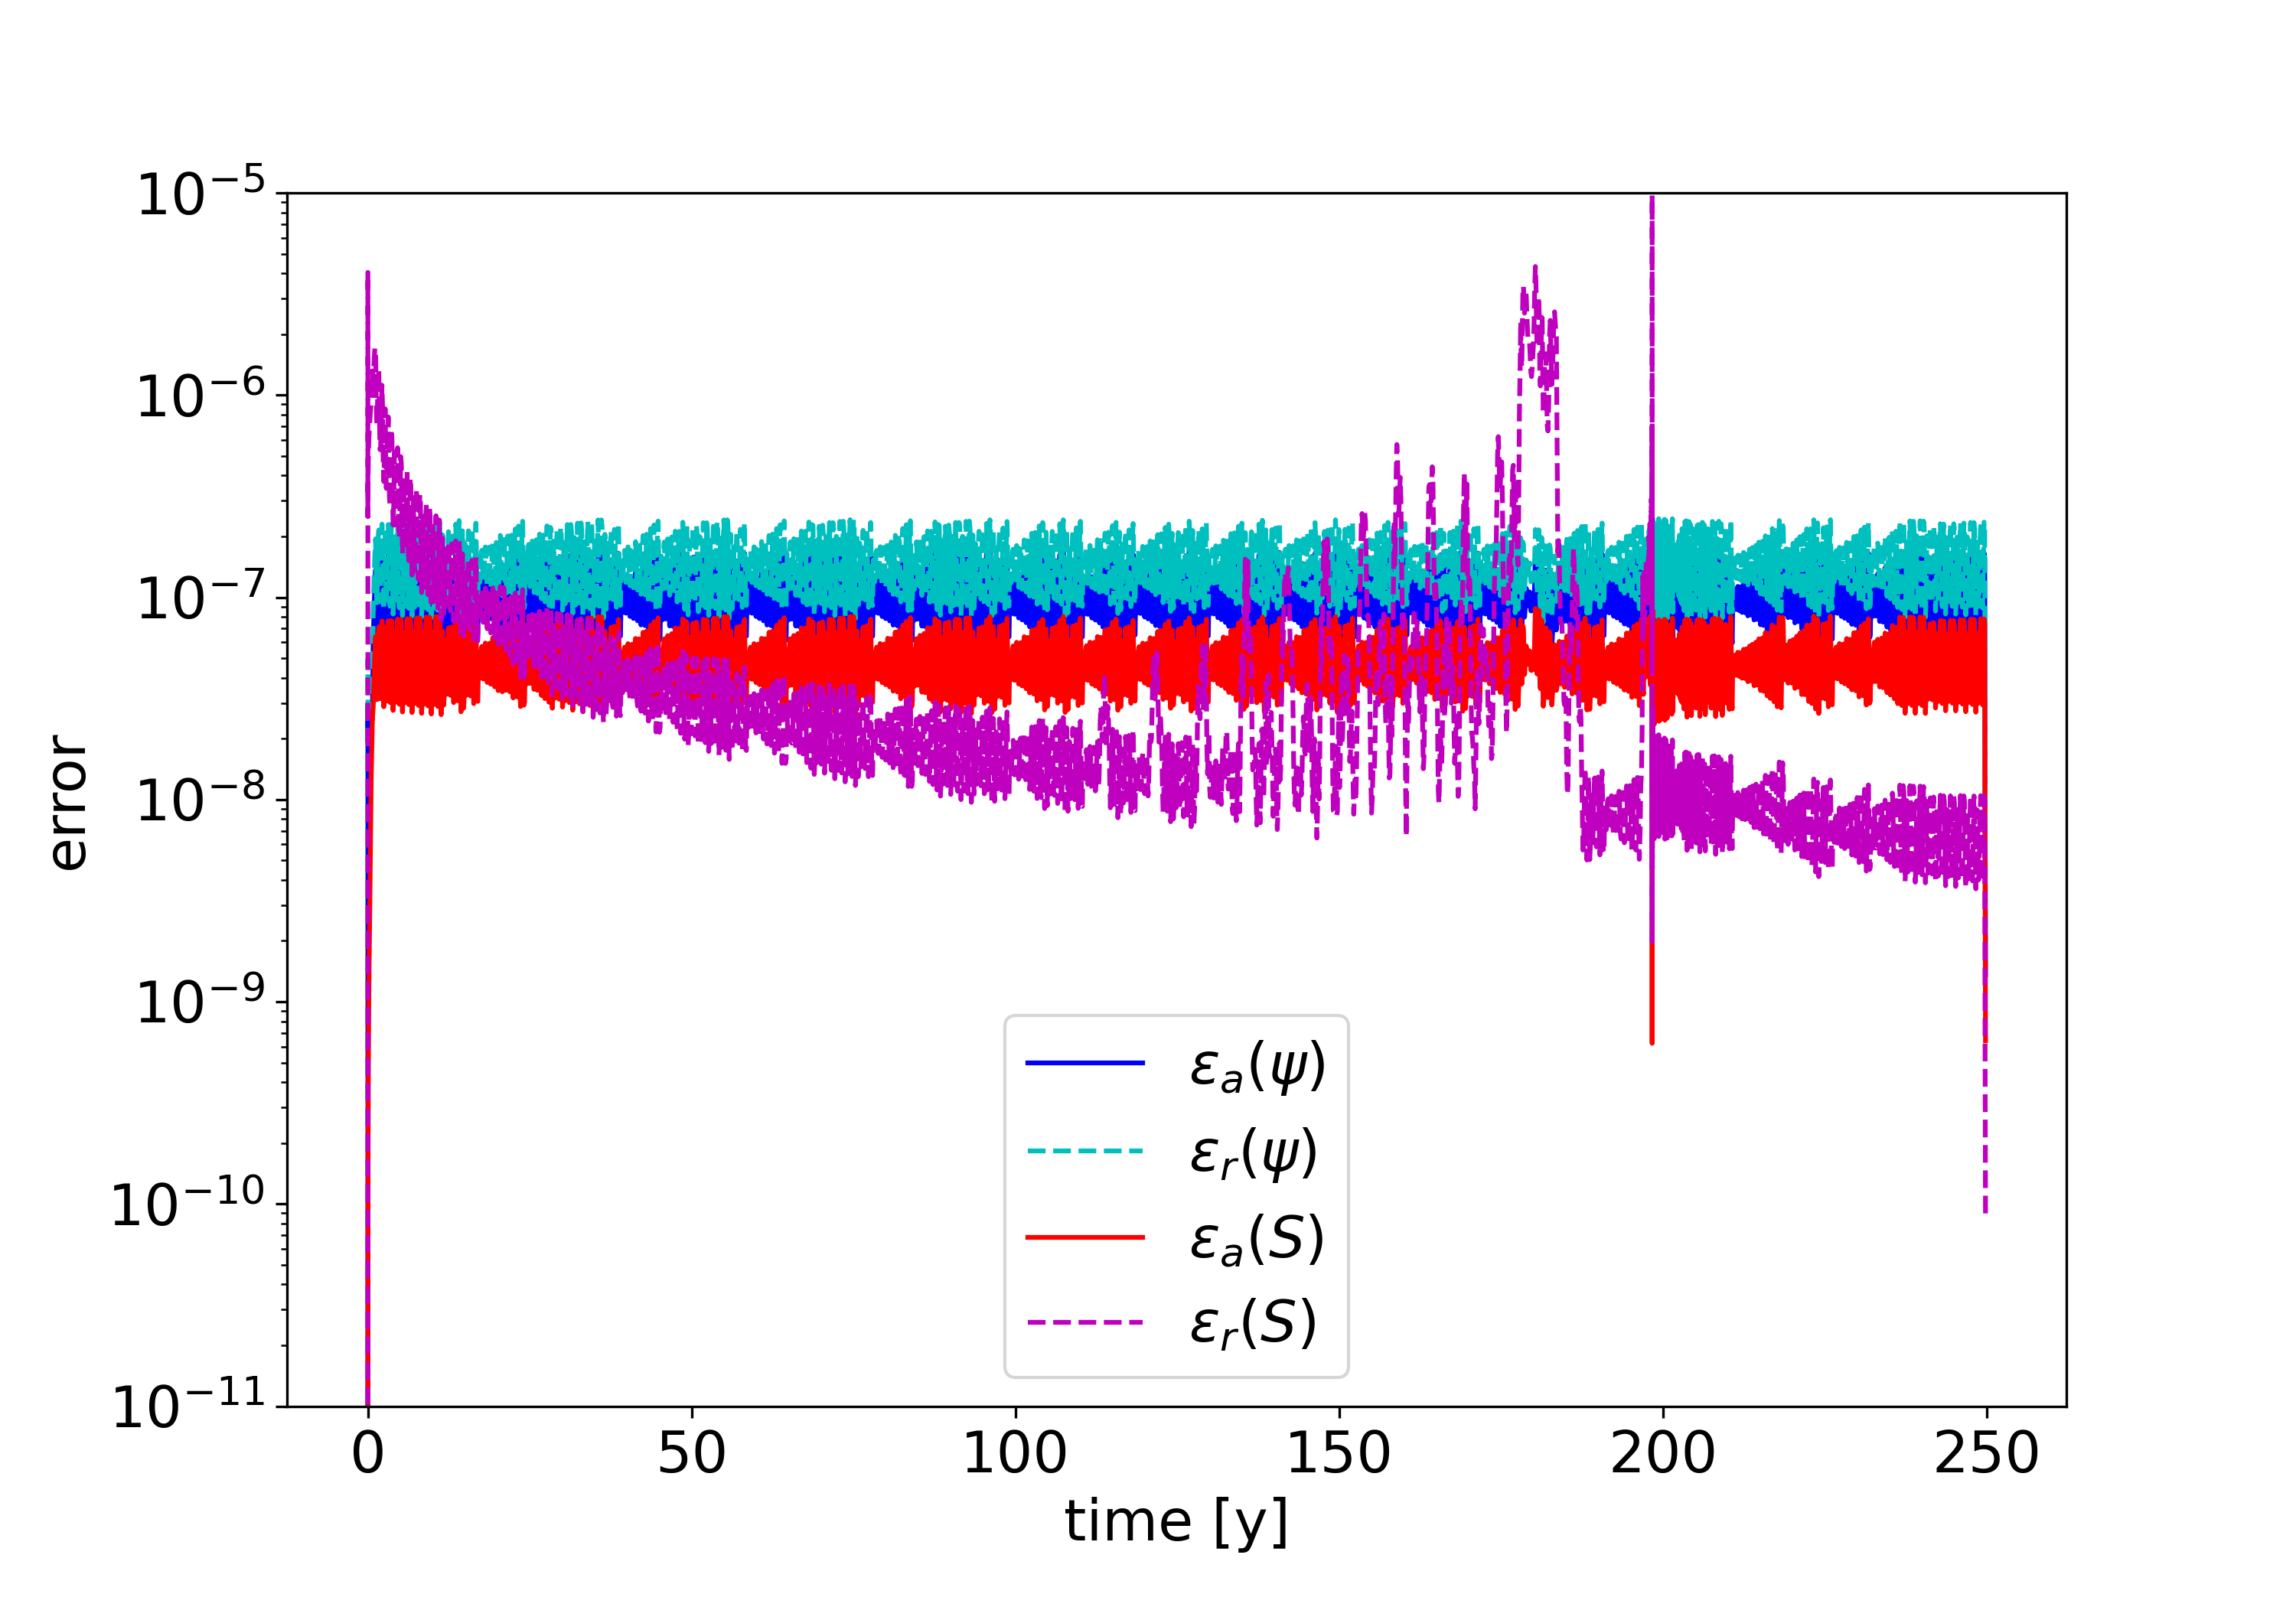
\includegraphics[width=0.6\textwidth]{images/TANDEMtimeEvolutionErrorall_RKDP5.png}
	\caption{Maximum relative and absolute errors using the RKDP5 method on a fault with 200 elements with an absolute and relative error tolerance of $10^{-7}$}
	\label{fig:errrors1e-7}
\end{figure}
Over the whole simulation time, the state variable $\psi$ takes values close to $0.8$ on all fault nodes, leading to a total tolerance for the corresponding components of $t_\psi \approx 1.8 \cdot 10^{-7}$. The blue line, which draws the maximum absolute error, is clearly limited by this tolerance value and the light blue line of the relative error is located, as expected, by a factor $1/0.8$ above the absolute error. \\
The error analysis of the slip presents a much less regular picture. The maximal absolute error lies always below the tolerance $t_S^a = 10^{-7}$, however the relative error reaches much higher values at the beginning of the simulation and before the earthquake event. The evolution of the extreme values of the slip in \autoref{fig:minmax1e-7} provides an explanation for these large errors. In the beginning, the slip at each node is below 1, thus the overall tolerance \\

\begin{figure}[H]
	\centering
	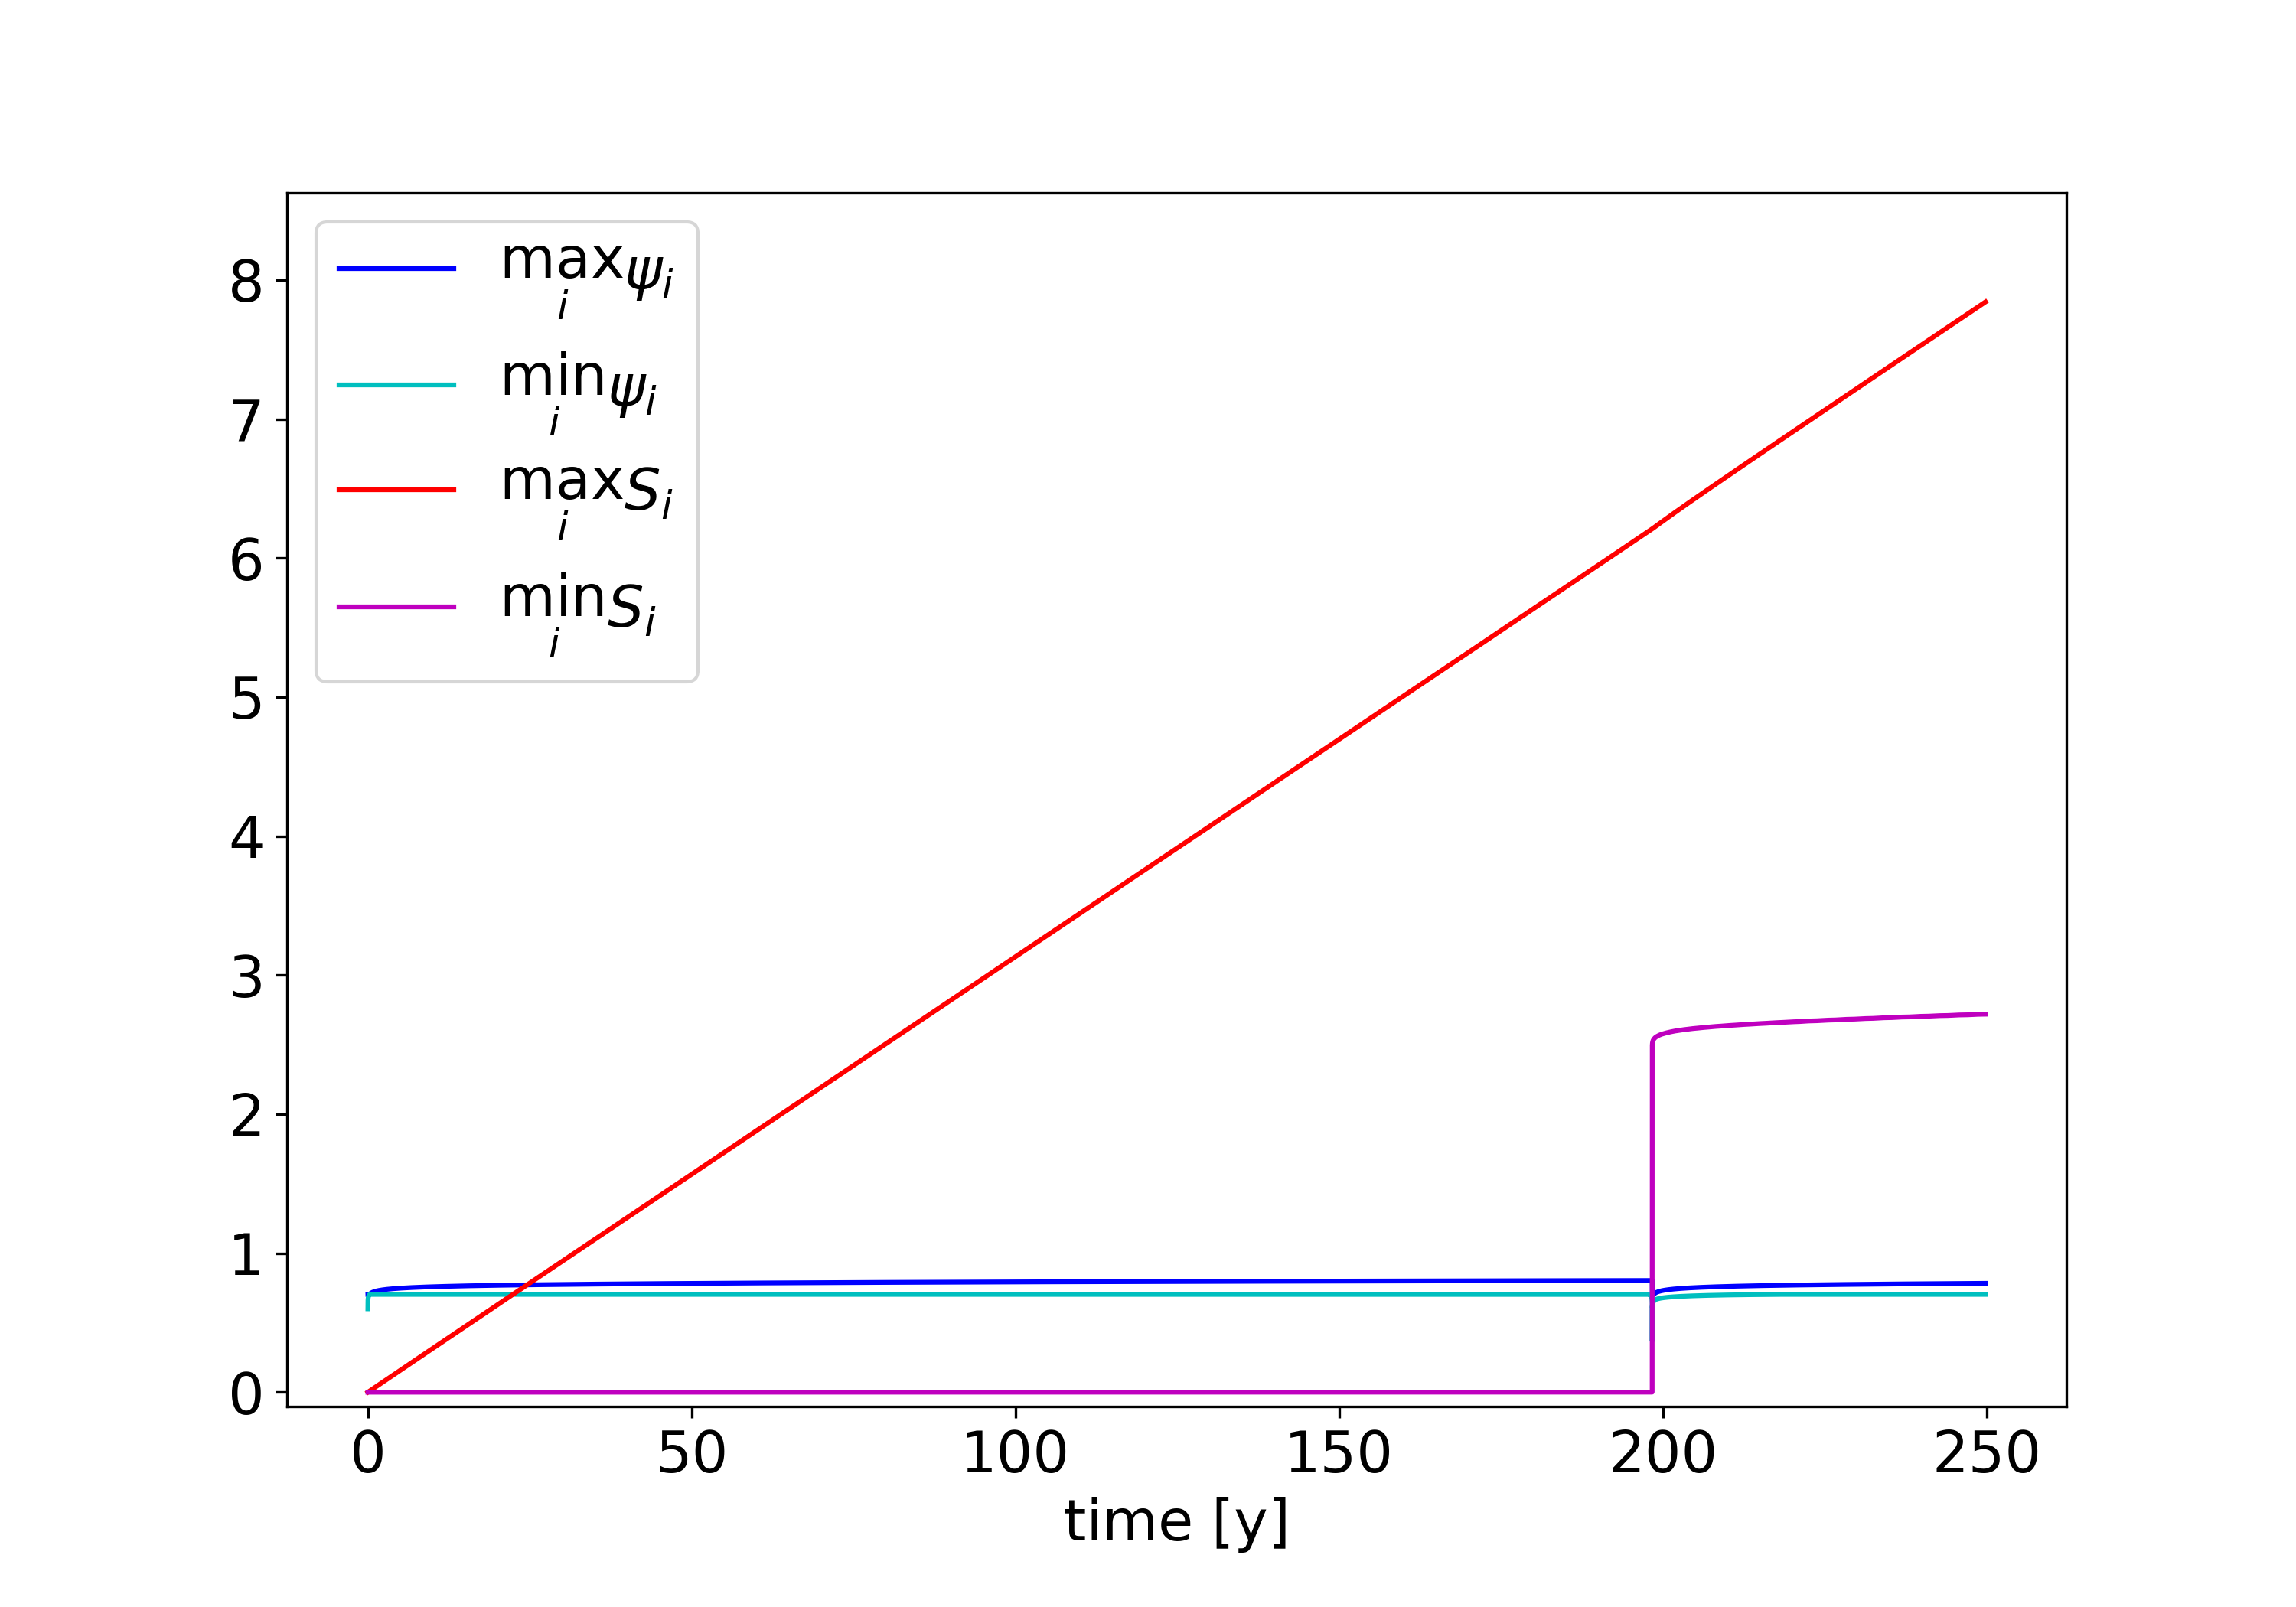
\includegraphics[width=0.6\textwidth]{images/TANDEMtimeEvolutionMinMaxAll_RKDP5.png}
	\caption{Maximum and minimum values of the state variable $\psi$ and of the slip $S$ over time. Simulation performed with the RKDP5 method on a fault with 200 elements with an absolute and relative error tolerance of $10^{-7}$}
	\label{fig:minmax1e-7}
\end{figure}

\subsubsection{Switching between different methods}
The simulation supports the use of different solvers and time integration methods for the aseismic slip phase and for the earthquake phase. To detect in which phase the simulation is currently in, the maximum slip rate $V_{max}$ at the current timestep is compared to the environment slip $V_0$. If $V_{max}>V_0$ is verified, it means that the simulation is currently in an earthquake, else wise it is in the aseismic slip. When the simulation detects a switch from one state to the other, and if a different problem formulation or integration method is defined by the users for both states, the program overwrites the PETSc configuration and restarts the solver at the current timestep with the new methods. It is thus possible, for instance, to use the compact DAE formulation for the aseismic slip and the 2nd order ODE formulation with an explicit Runge-Kutta scheme for the earthquake. 

\subsection{Newton Iteration}
\label{ssec:ConvergenceNewtonIteration}
The Jacobian matrix is needed to apply implicit numerical methods to the SEAS problem. Unlike explicit methods, they evaluate the right hand side of the ODE with the current solution which is not known yet. To calculate the solution vector at a given time step, a nonlinear algebraic equation of the form $\phi(x) = 0$ needs to be solved where $x$ is the solution vector to be determined. The Newton method is often used to solve the equation because of its ease to implement and its second-order convergence. 

\begin{itemize}
	\item Calculate an initial guess $x_0$
	\item Repeat until tolerance is reached $\|\phi(x_n)\| < TOL$: 
	\begin{itemize}
		\item $x_{n+1} = x_n - J_\phi^{-1}(\phi(x_n)) \phi(x_n)$
	\end{itemize} 
\end{itemize}

The matrix $J_\phi^{-1}(f(x_n))$ is the Jacobi matrix of the function $\phi$ evaluated at the point $x_n$. \\

\subsubsection{Convergence}
Next, the convergence properties of the Newton iteration with the analytic Jacobian is investigated on the 1st order ODE formulation. For this, we solve one timestep of the implicit Euler method starting from the initial condition of the simulation. The function $\phi$ and its Jacobian matrix are given by: 
\begin{align}
\phi(x) &= -x + x^{(0)} + h F(x) \\
J_\phi(x) &= -I + h J_F(x)
\end{align}
The vector $x$ contains both the components related to the slip $S$ and to the state variable $\psi$ and the right hand-side vector $F(x)$ contains their respective time derivative. The Jacobian of the proposed Newton iteration needs the Jacobian $J_F(x)$ of the right-hand side vector, of which the correctness is evaluated here. The success of the Newton iteration, thus observable second-order convergence, indicates the correctness of the Jacobian matrix. \\
Furthermore, the behavior of the analytic expression of the Jacobian is compared to the behavior of an iterative approximation of it. The Broyden's method \cite{BroydenIteration} provides an enhancement of the Newton method which updates the Jacobian matrix at each iteration without the need of its analytical expression. The main difficulty is to find an appropriate initial guess to achieve a fast convergence. 

\begin{itemize}
	\item Calculate the initial guesses $x_0$ and $J_0$
	\item Repeat until tolerance is reached $\|\phi(x_n)\| < TOL$: 
	\begin{itemize}
		\item $\Delta x_n = x_n - x_{n-1}$ and $\Delta \phi_n = \phi(x_n) - \phi(x_{n-1})$ 
		\item $J_n = J_{n-1} + \frac{\Delta \phi_n - J_{n-1}\Delta x_n}{\|\Delta x_n\|^2} \Delta x_n^T$
		\item $x_{n+1} = x_n - J_n \phi(x_n)$
	\end{itemize} 
\end{itemize}

The motivation behind this update scheme is to minimize the Frobenius norm $\|J_n - J_{n-1}\|_F$. As a matter of simplicity, the initial guess of the Jacobian is obtained with the analytical expression of it, even though its correctness has not yet been shown. Other initialization methods such as finite differences do not lead to convergence of the Broyden method. \\
The experiment has been performed on a symmetric, two-dimensional domain of varying size. The initial guesses for $x$ are obtained with one step of the explicit Euler method with a timestep of $h = 10^5$s. This time step is large enough to obtain an error to the exact value at this time which needs several Newton iterations to be corrected but still small enough to ensure that the Newton iteration converges at all. The evolution of the residual $\phi(x_n)$ is shown in \autoref{fig:convergenceNewtonAndBroydenDifferentSizes}.
\begin{figure}[H]
	\centering
	\begin{subfigure}{0.32\textwidth}
		\centering
		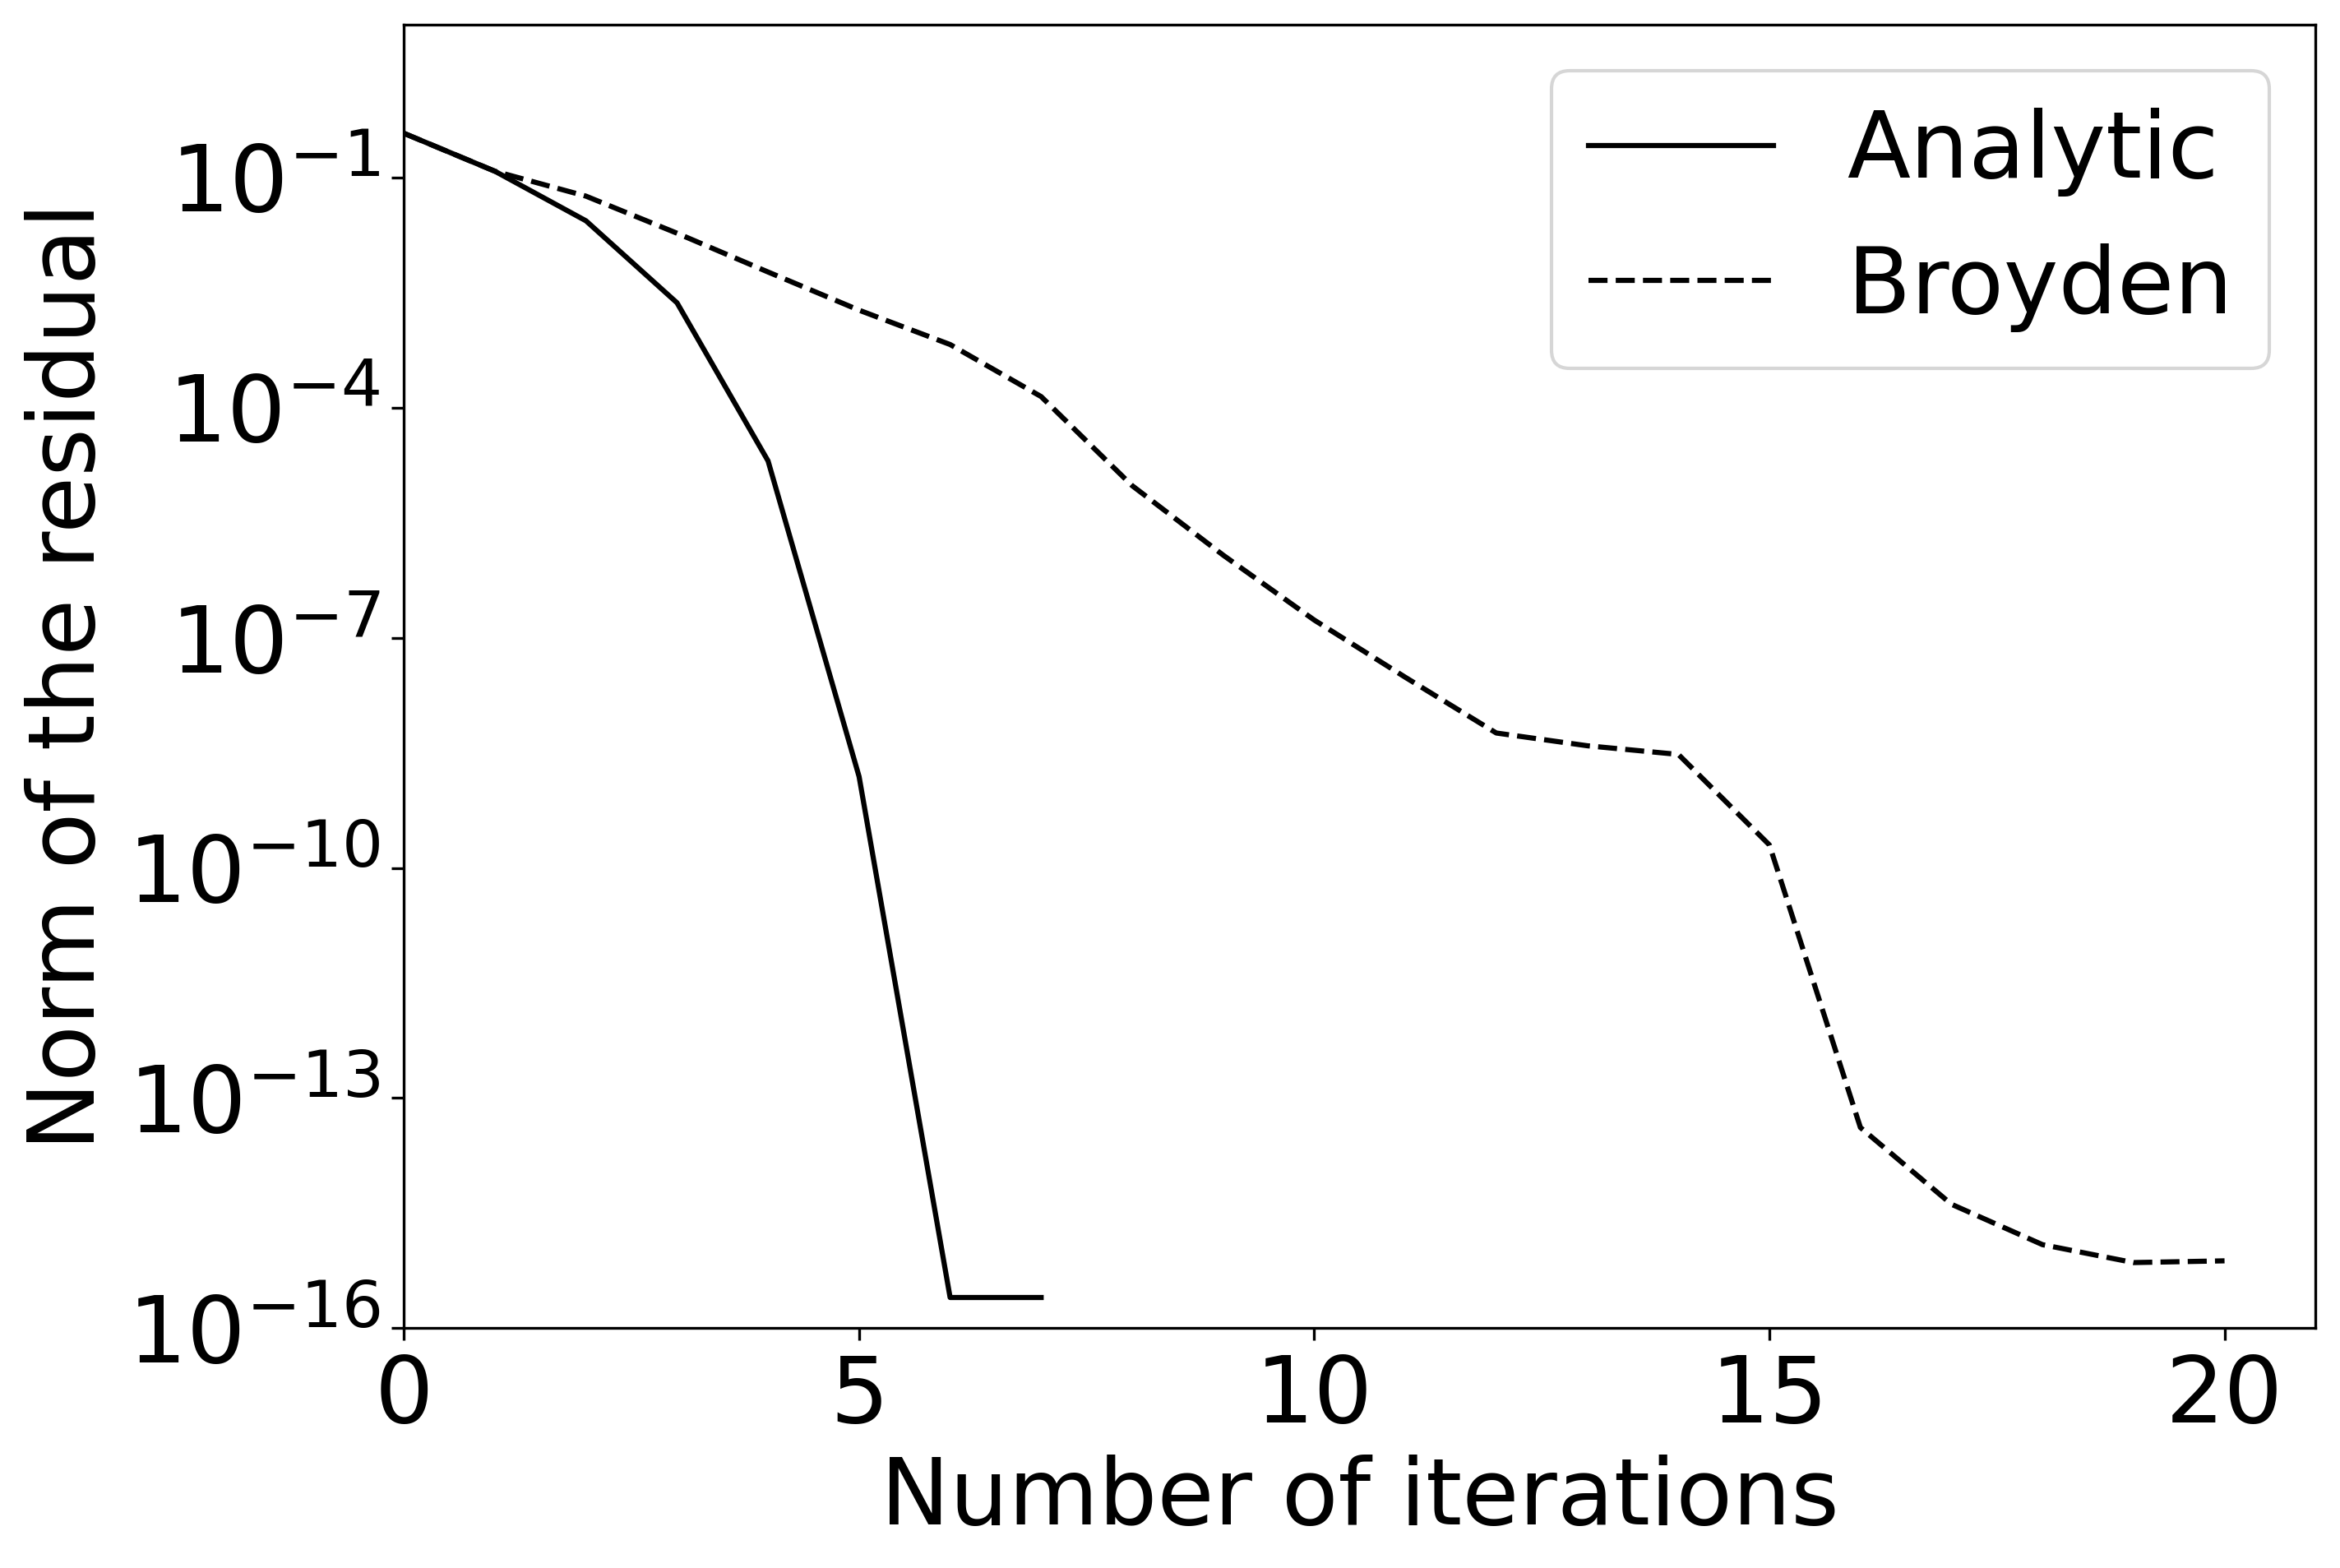
\includegraphics[width=0.9\textwidth]{images/NewtonIterationConvergence5Elements.png}
		\subcaption{5 fault elements} 
	\end{subfigure} 
	\begin{subfigure}{0.32\textwidth}
		\centering
		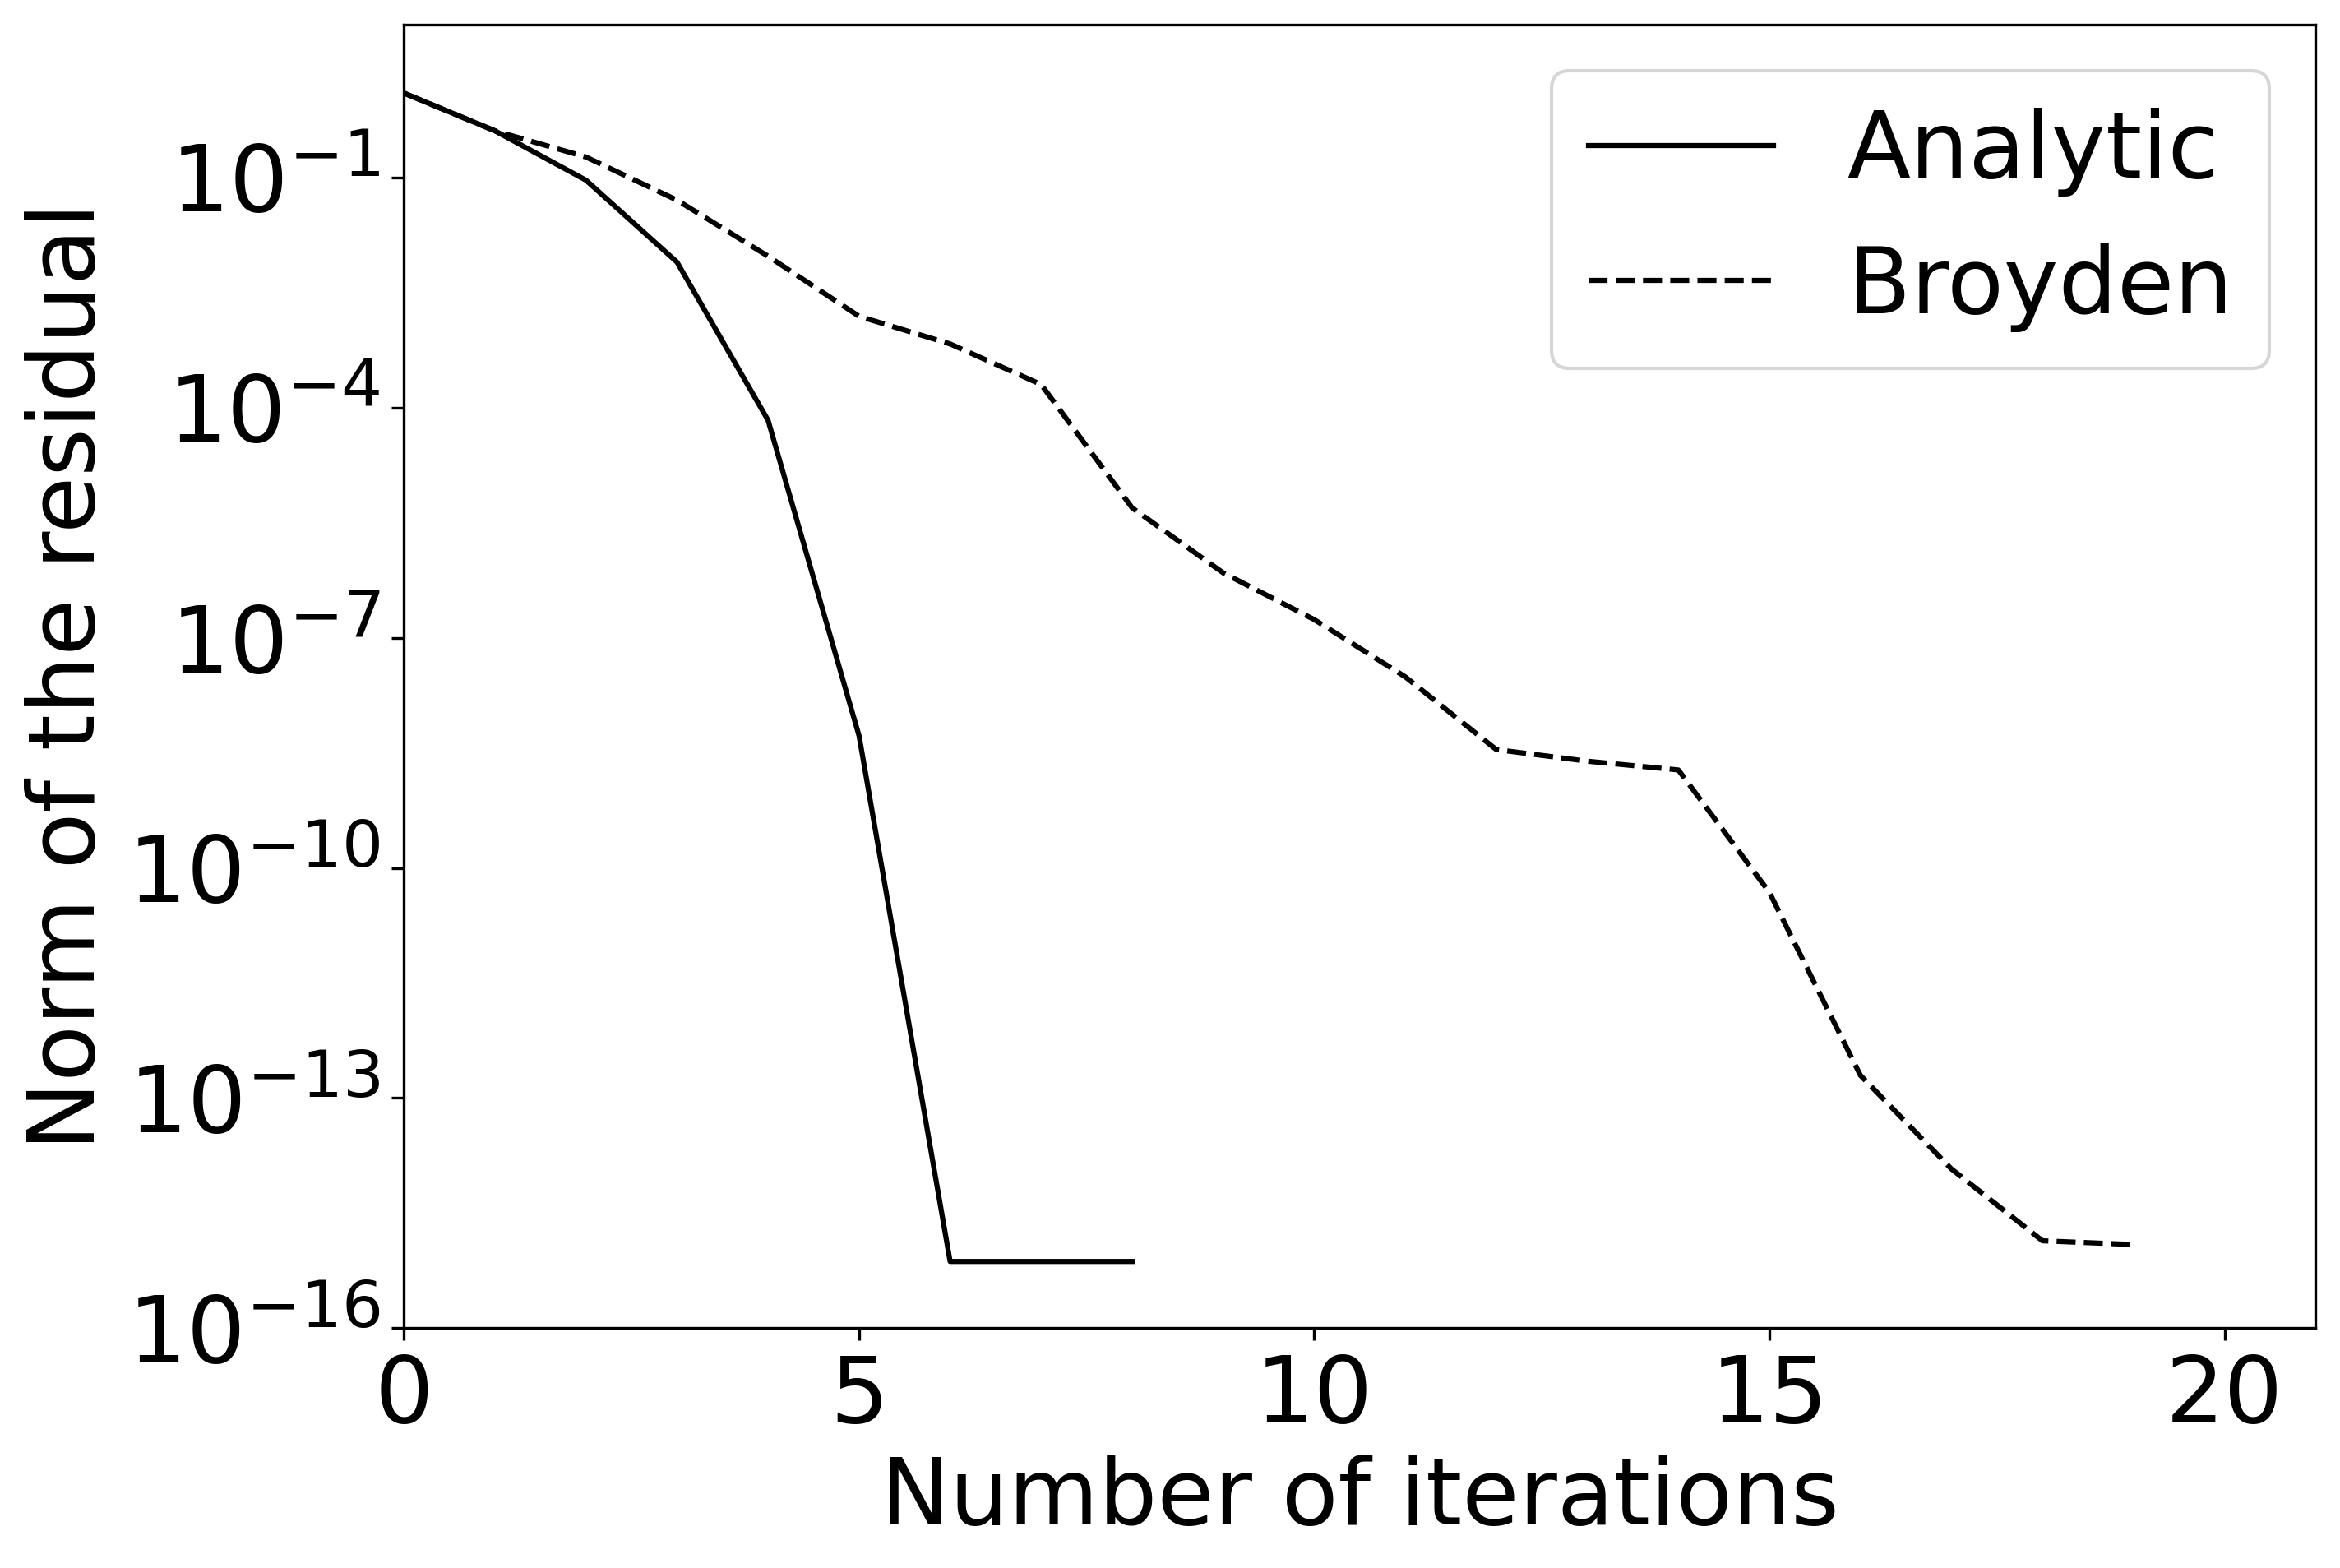
\includegraphics[width=1\textwidth]{images/NewtonIterationConvergence40Elements.png}
		\subcaption{40 fault elements} 
	\end{subfigure}
	\begin{subfigure}{0.32\textwidth}
		\centering
		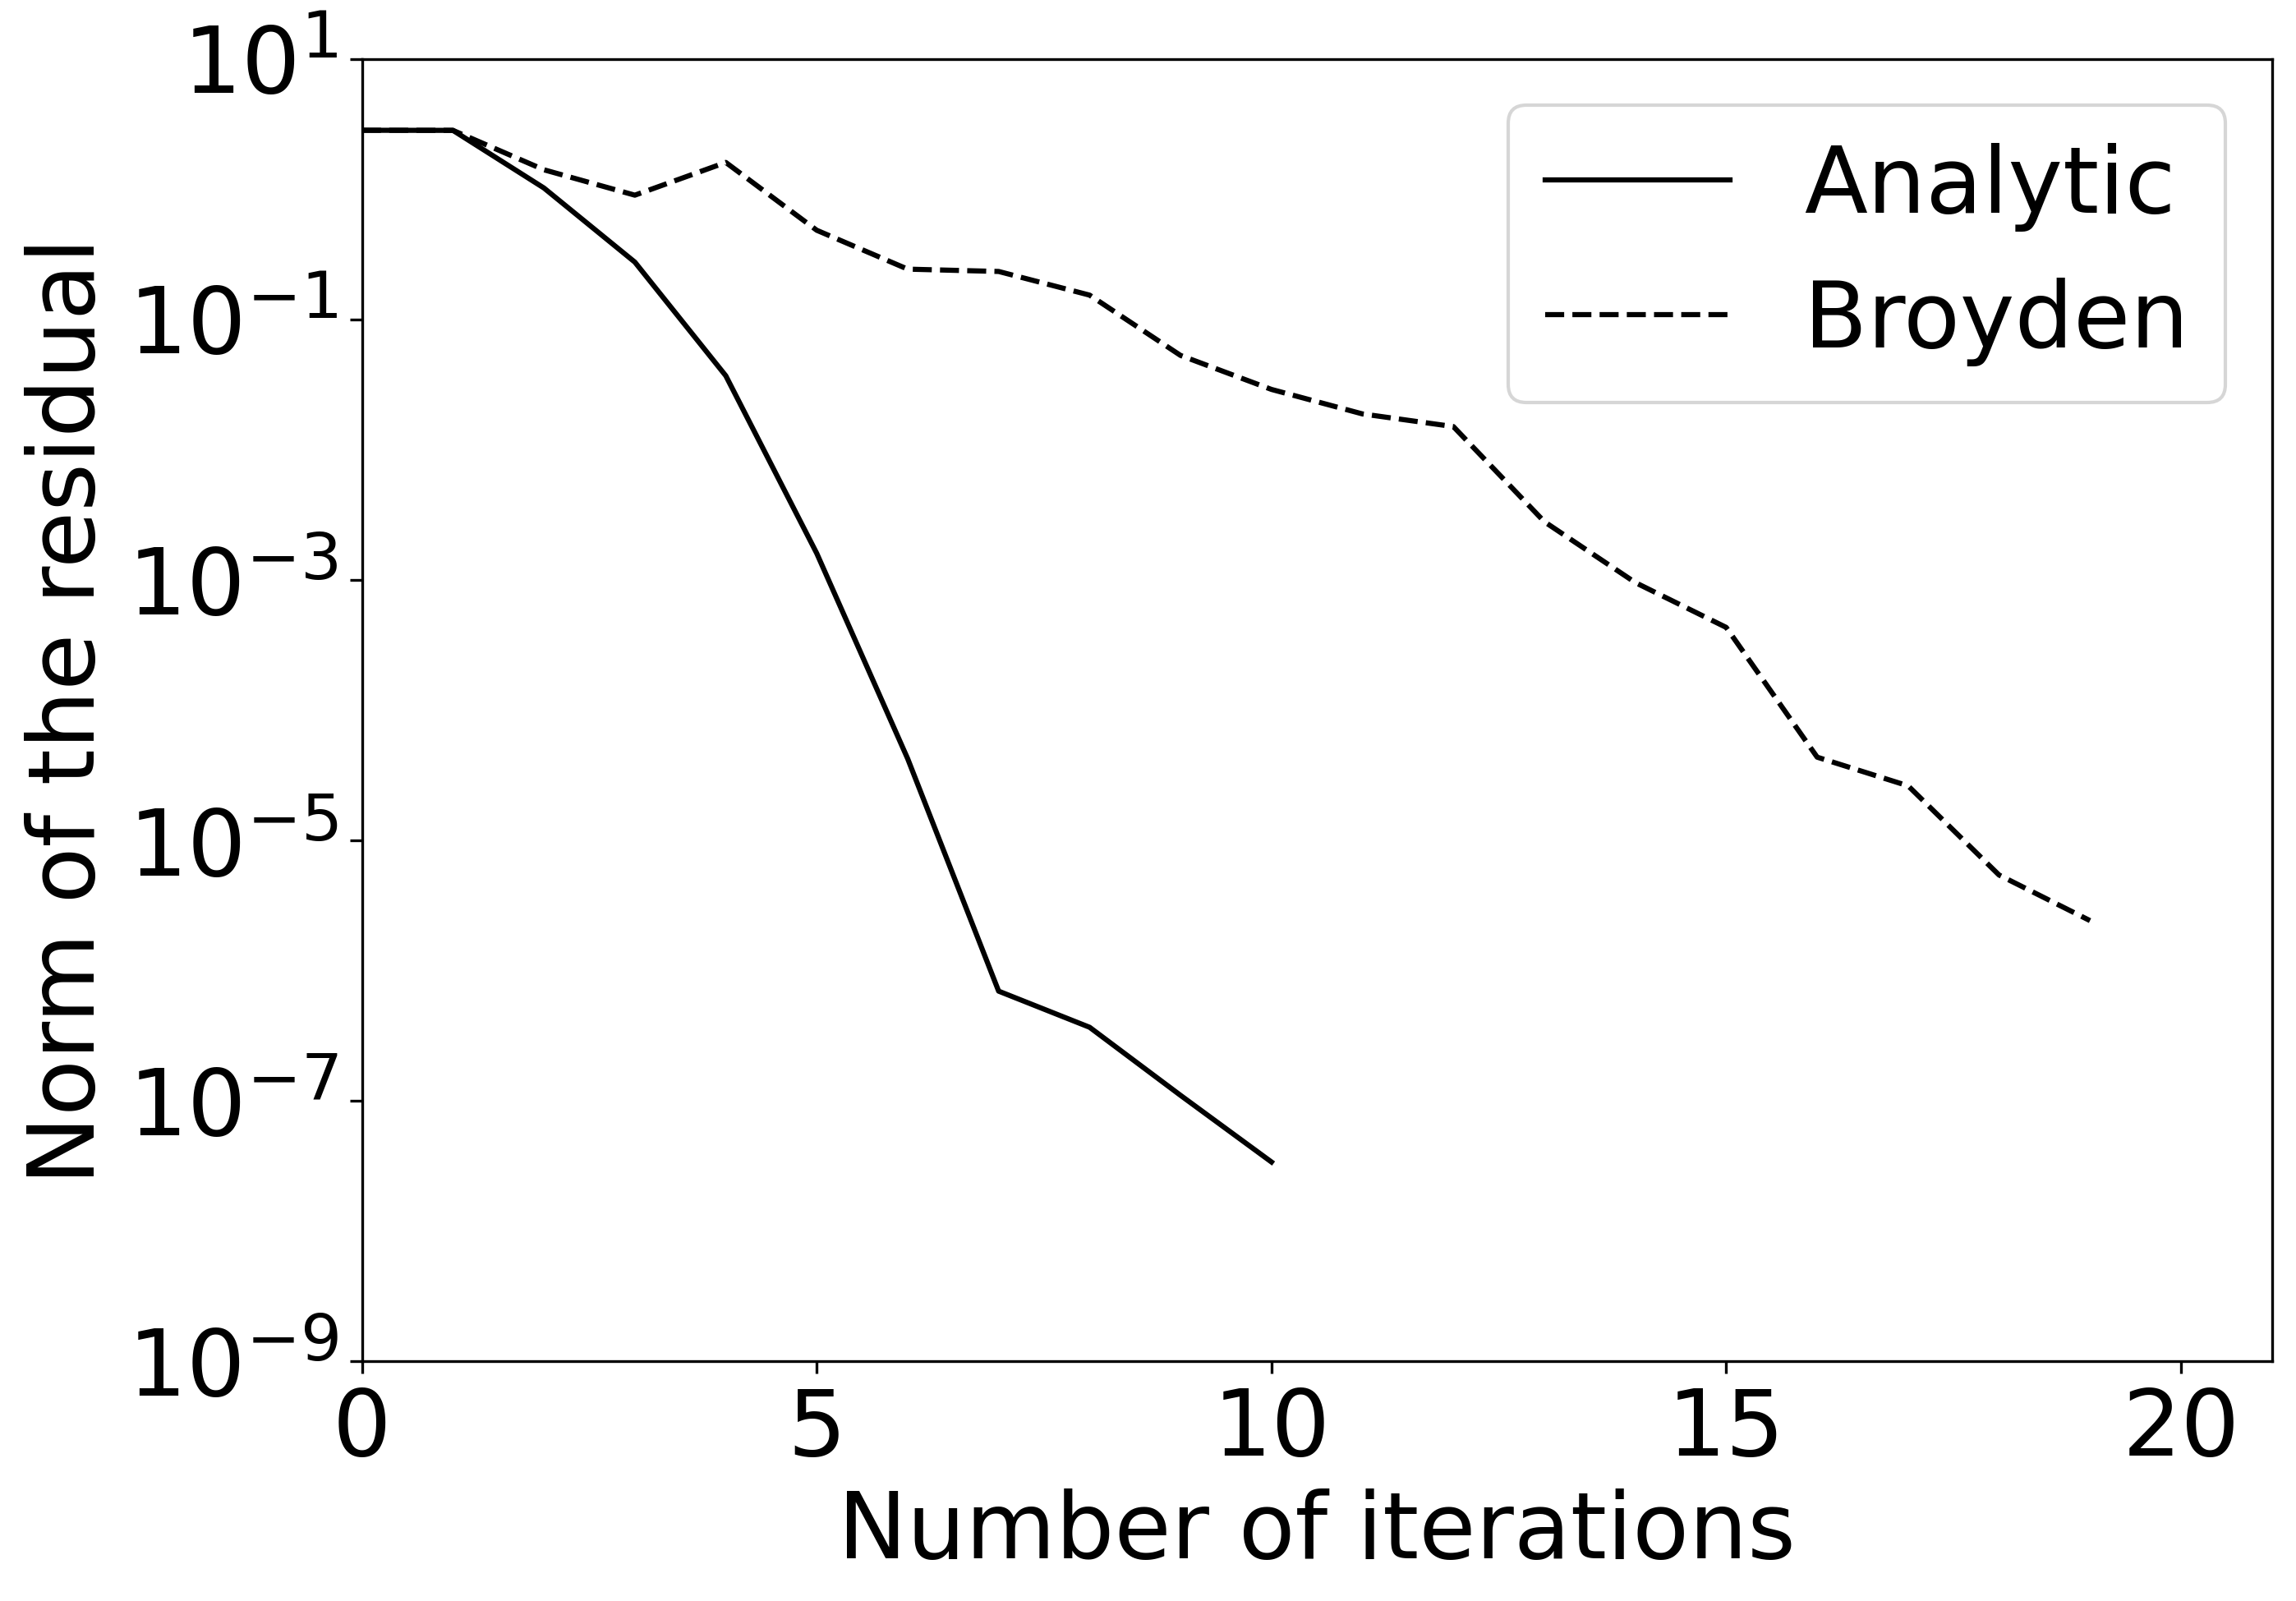
\includegraphics[width=1\textwidth]{images/NewtonIterationConvergence200Elements.png}
		\subcaption{200 fault elements} 
	\end{subfigure}
	\caption{Evaluation of the L2 norm of the residual $\phi(x_n)$ at each iteration of the Newton and Broyden methods}
	\label{fig:convergenceNewtonAndBroydenDifferentSizes}
\end{figure}
It can be immediately seen that the Newton method with an analytic expression of the Jacobian reaches much faster the maximum reachable accuracy of about $10^{-15}$ as if it was approximated with the Broyden method. The convergence rate even seems to be quadratic, as one would expect for the Newton iteration and the convergence is similarly fast for all tested domain sizes. The Broyden method on the other hand shows rather a linear convergence behavior, and the number of needed iterations increases with problem size. This makes the Broyden iteration particularly unsuitable for simulations on large domains. The approximated Jacobian matrix at the end of the Broyden iteration matches with high precision its analytic counterpart, since the maximum relative difference among the entries is of the order of $10^{-5}$. \\
So far, it has been shown that the Newton iteration converges well for various domain sizes. The chosen timestep size $10^5$s is still small, as in the aseismic slip, it may reach the order $10^7$s. \autoref{fig:convergenceNewtonAndBroydenDifferentTimeSteps} shows the norm of the residual for the timestep sizes $10^5$s $10^6$s and $10^7$s. The direct iteration with the analytic Jacobian matrix always has a quadratic convergence, and the slightly higher number of iterations for large timesteps is essentially due to the worse initial guess. In contrast, the Broyden iteration converges much slower if the timestep size increases. 
\begin{figure}[H]
	\centering
	\begin{subfigure}{0.45\textwidth}
		\centering
		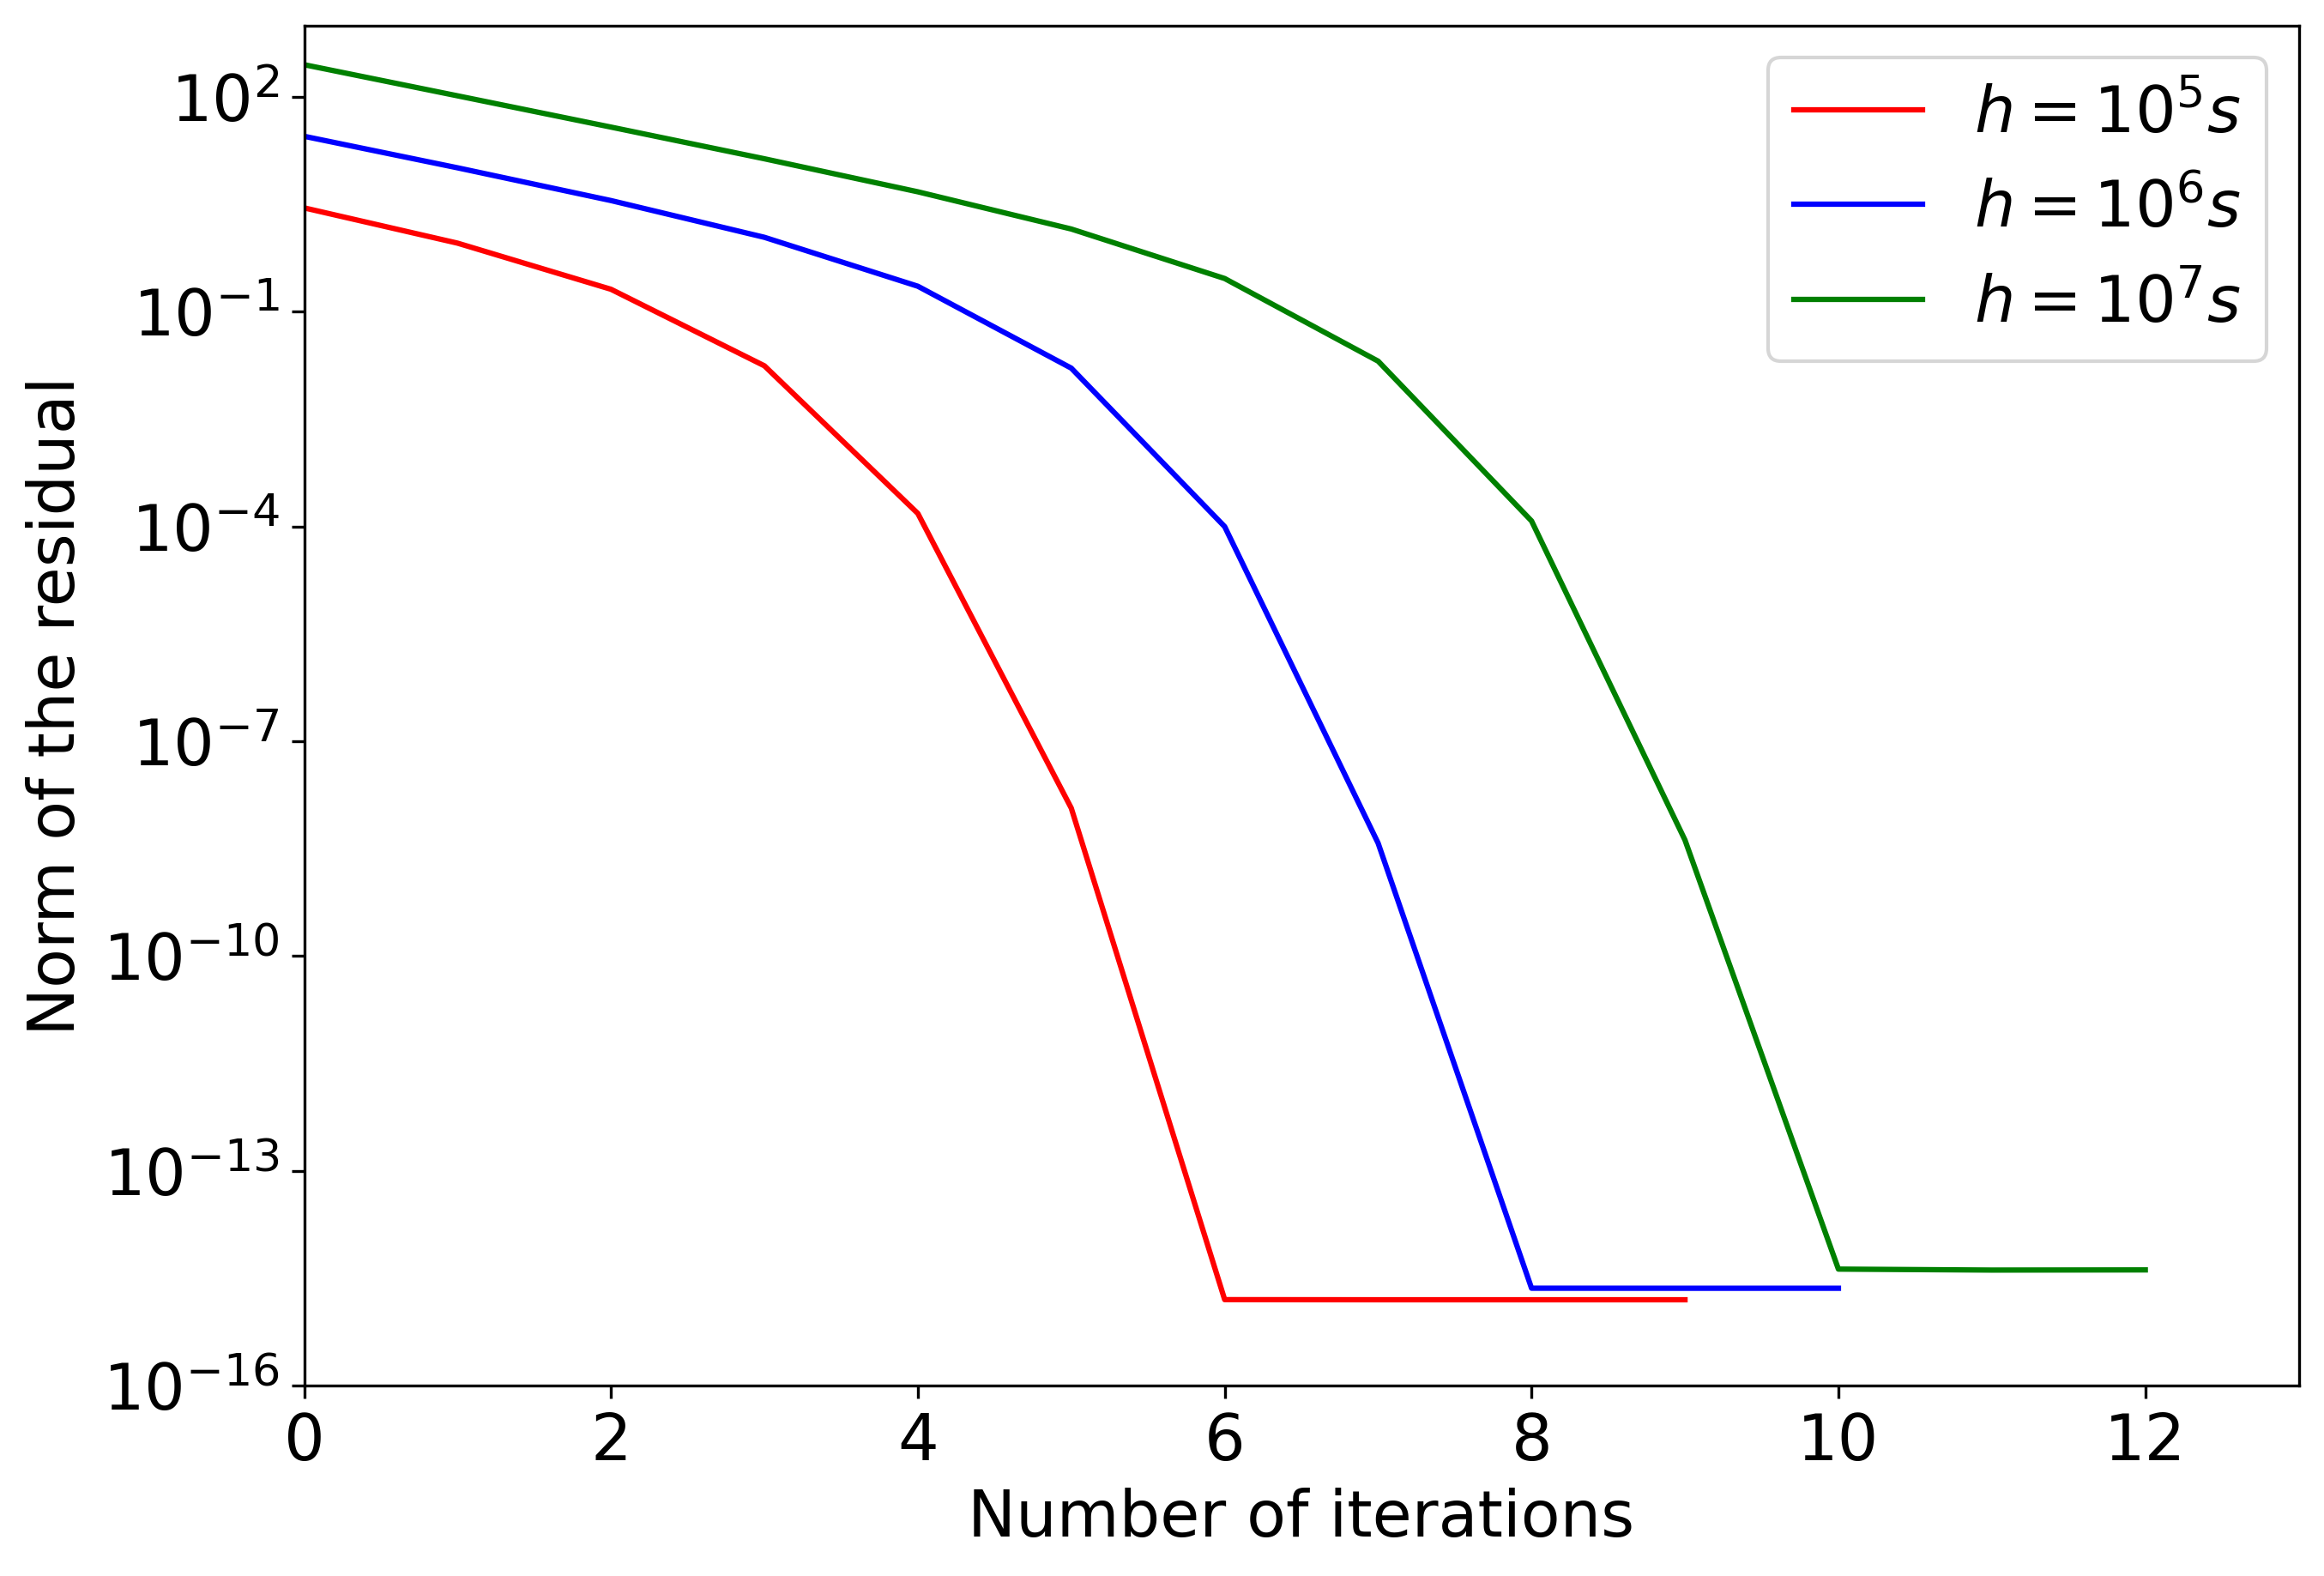
\includegraphics[width=1\textwidth]{images/NewtonIterationConvergence200Elements_DifferentDT_Analytic.png}
		\subcaption{Direct iteration}
	\end{subfigure}
	\begin{subfigure}{0.45\textwidth}
		\centering
		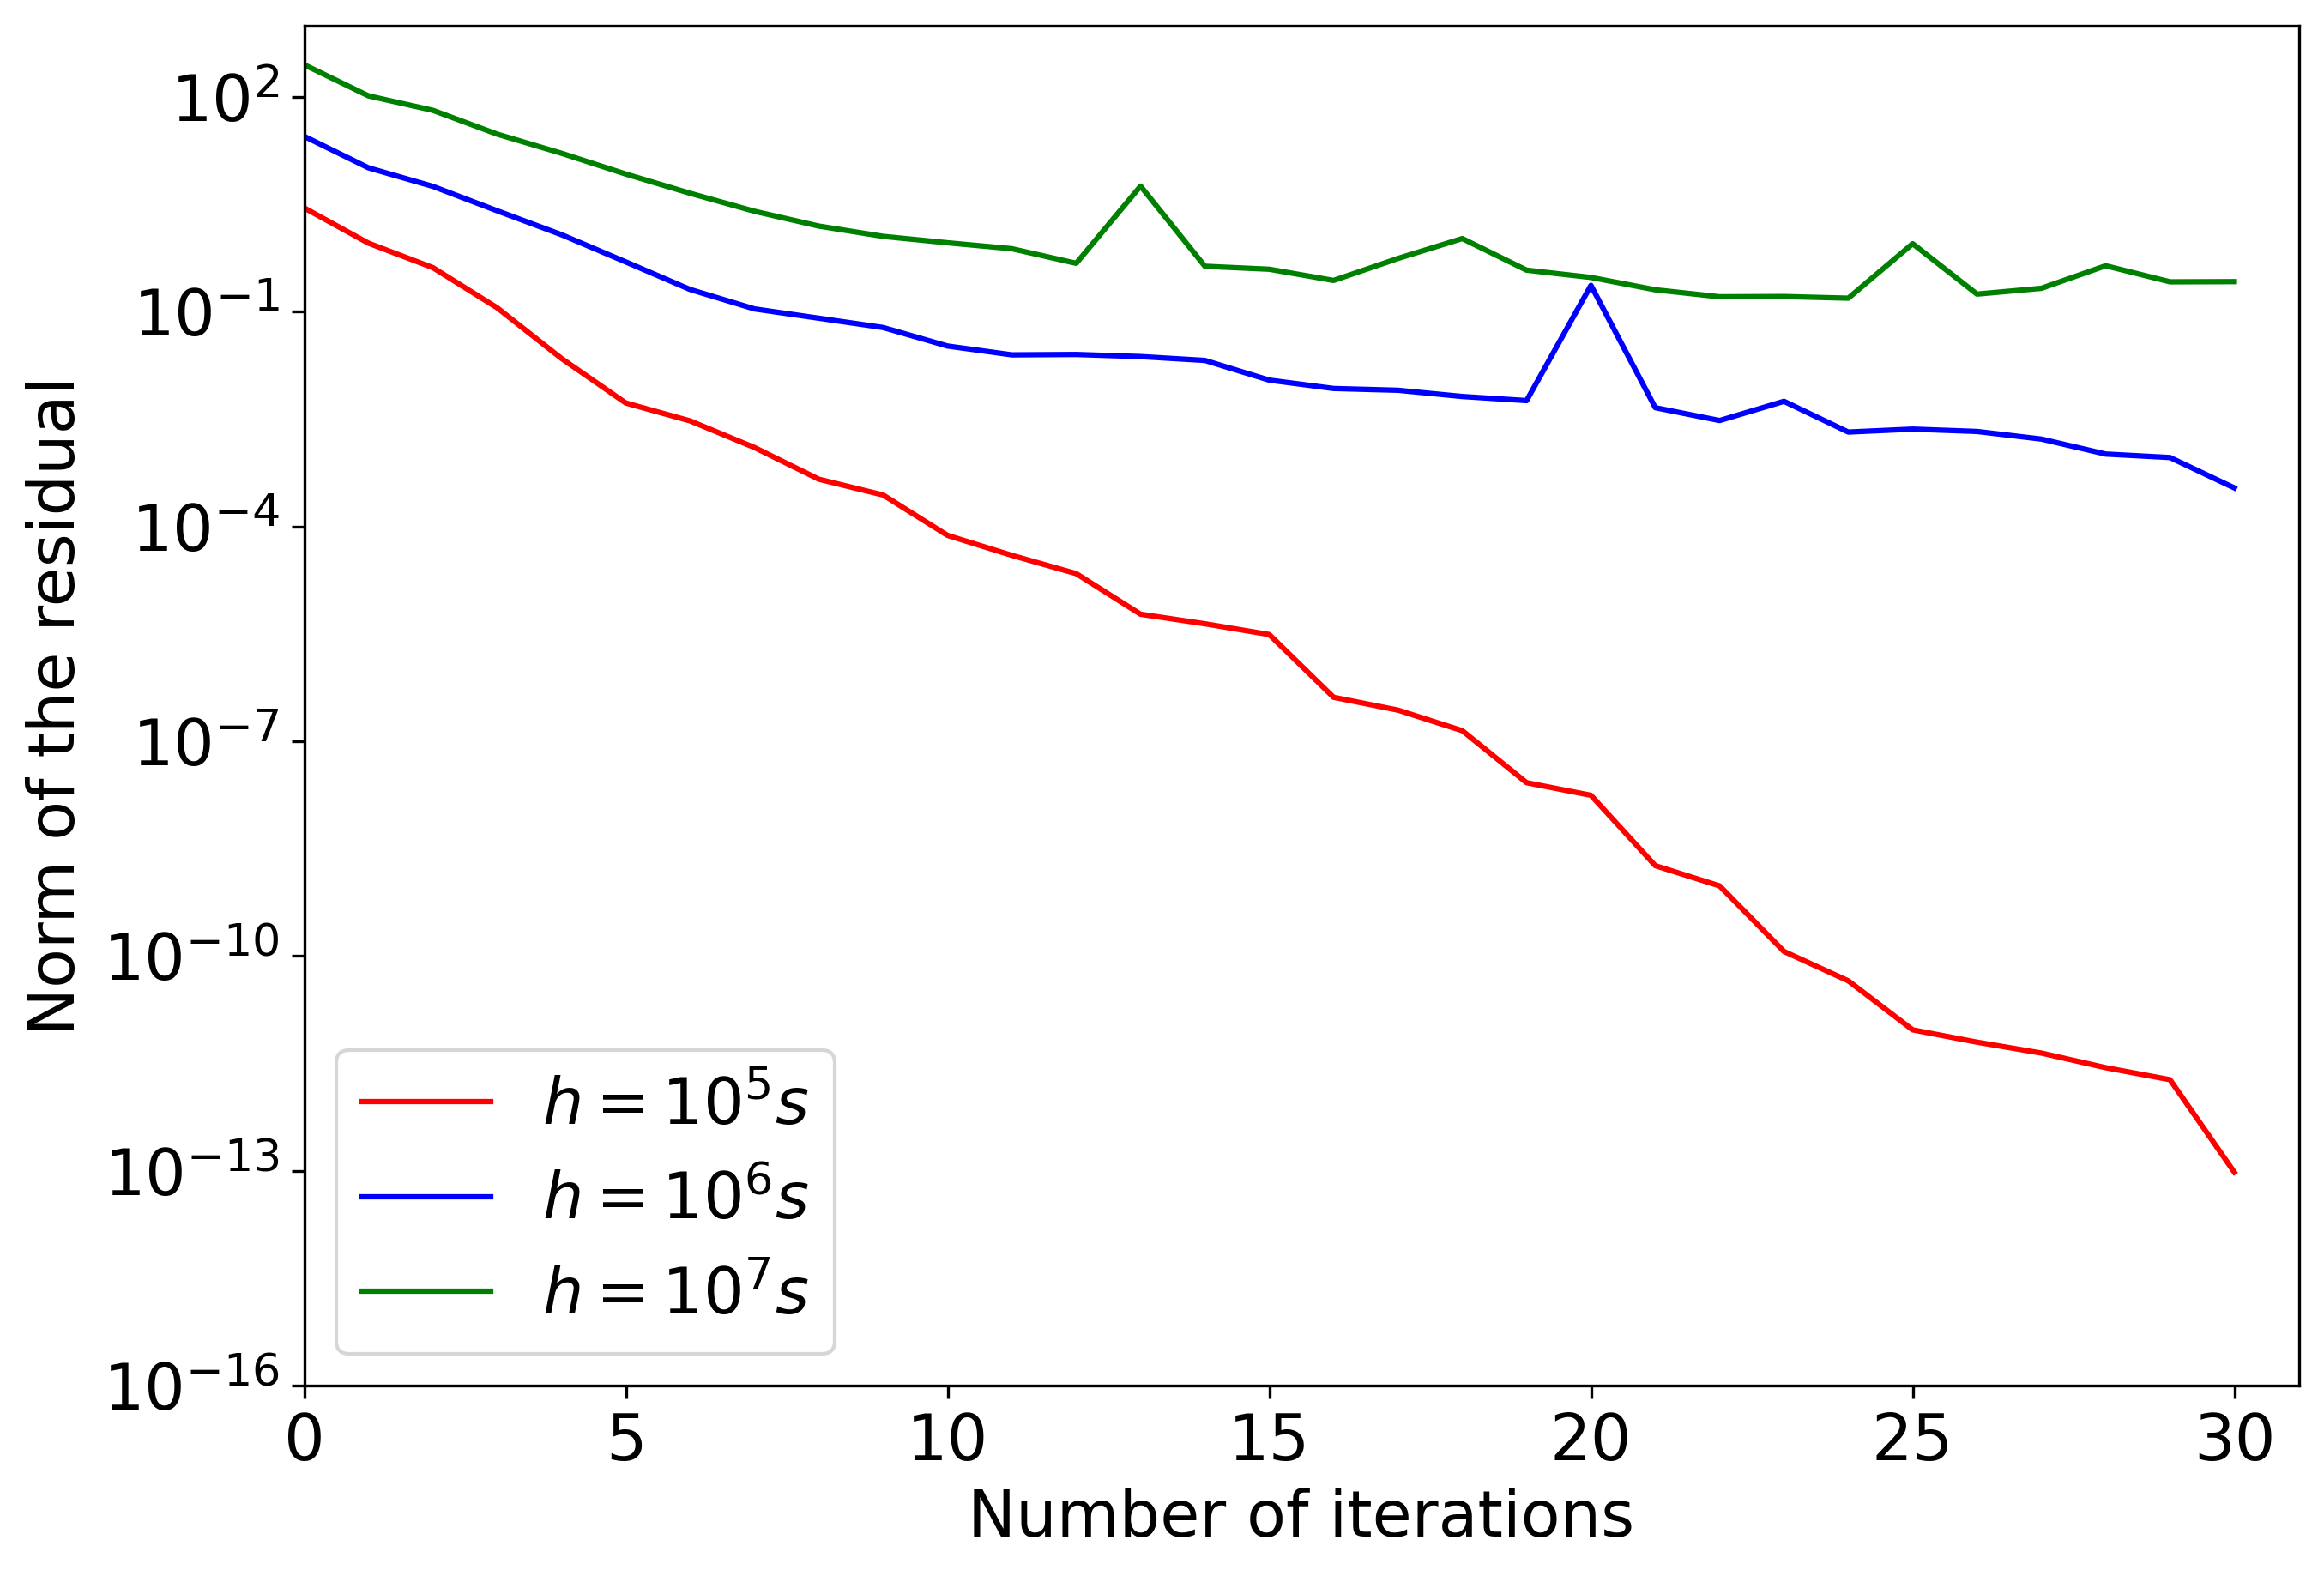
\includegraphics[width=1\textwidth]{images/NewtonIterationConvergence200Elements_DifferentDT_Broyden.png}
		\subcaption{Broyden iteration}
	\end{subfigure}
	\caption{Evaluation of the L2 norm of the residual $\phi(x_n)$ at each iteration of the Newton and Broyden methods for 200 fault elements}
	\label{fig:convergenceNewtonAndBroydenDifferentTimeSteps}
\end{figure}

It could be shown that the Newton iteration with the analytic Jacobian has excellent convergence properties for any domain sizes and large time step sizes. On the other hand, the alternative with a Broyden iteration, which approximates the Jacobian matrix along with the solution, converges only very slowly for large domains and large timesteps which is why this method is not suited to solve the problem. In practice, the  Newton iteration converges much faster because BDF schemes of higher order are used instead of the implicit Euler and the initial guess at the beginning of the iteration is obtained by extrapolating the previous solution vectors to the current simulation time. Usually, one Newton step is required to achieve the desired accuracy, which means two evaluations of the right-hand side function. \\

\subsubsection{Convergence issues with the compact DAE formulation}
The compact DAE formulation from \autoref{eq:DAE_compact_formulation_SEAS} shows a similar convergence behavior only during the aseismic slip. Whereas the method never diverges, the maximal achievable accuracy depends on the current time step size, in a way that for very small timesteps, the residual in the Newton iterations does not go below some large value. This bad convergence can be seen in \autoref{fig:convergenceIssuesCompactDAENewtonIterations}, which shows the infinity norm of the residual at each Newton step for different time step sizes. The largest instance, of the order $10^7$, is representative for the aseismic slip after the first earthquake and the other samples have been taken in the initial phase of the second earthquake, when the slip rate increases significantly and the timestep size decreases. \autoref{fig:convergenceIssuesCompactDAEMaxResidual_vs_dt} shows the maximum residual at the end of the Newton iteration in function of the current timestep size for all timesteps in the simulation. The locations of the samples in the first graph are highlighted by colored points. It can be clearly seen that a large residual norm inversely depends on the timestep size. \\ 
To obtain these results, the time integration itself has not been performed with the compact DAE formulation, since it obviously yields a poor accuracy, but rather with the 1st order ODE formulation using a classic adaptive RK4 scheme. At each timestep, the Newton iteration has been launched until the residual norm does not decrease anymore and the final result was discarded. Therefore, the solution vectors at the previous timesteps needed in the BDF method stem from the explicit RK4 time integration and thus slightly differ to the vectors in the time integration with the compact DAE formulation. To discuss the convergence, this difference is not significant, since the convergence issues arise in either case. \\

\begin{figure}[H]
	\centering
	\begin{subfigure}[t]{0.32\textwidth}
		\centering
		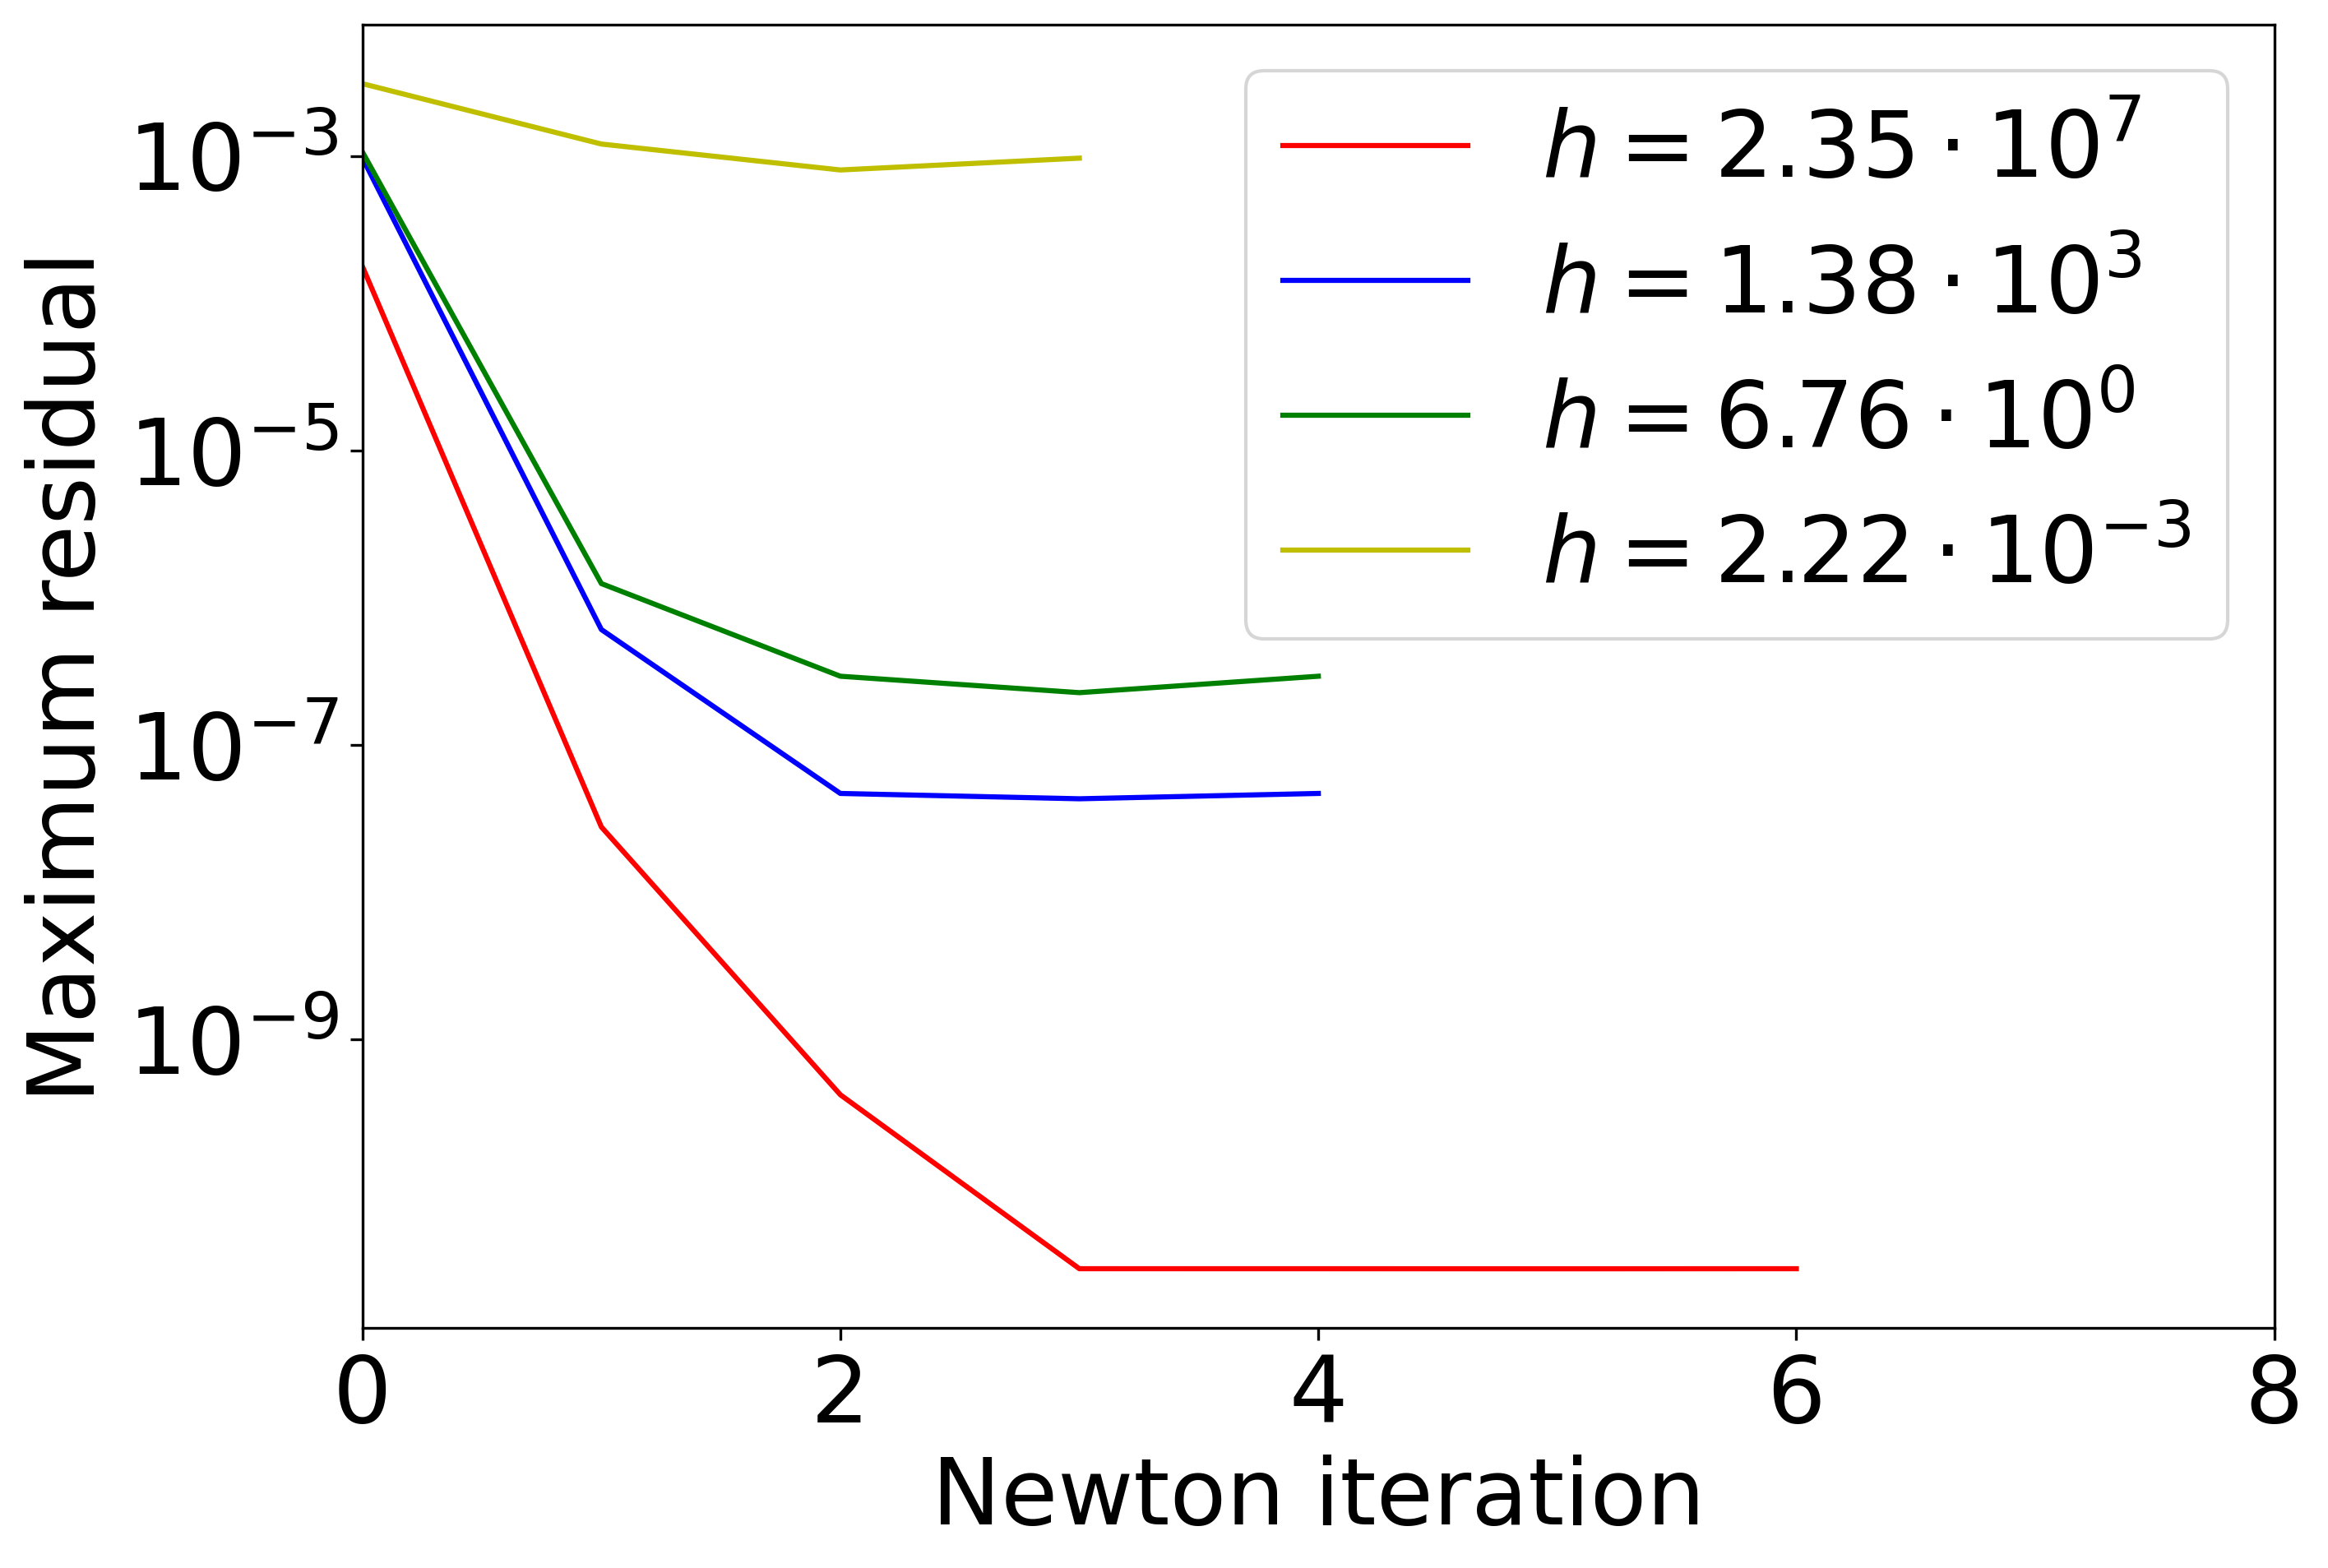
\includegraphics[width=0.9\textwidth]{images/TANDEMConvergenceAnalysisCompactDAENewton_Size5.png}
		\subcaption{$\infty$-norm of the residual in the Newton iterations at different time step sizes} 
		\label{fig:convergenceIssuesCompactDAENewtonIterations}
\end{subfigure} 
	\begin{subfigure}[t]{0.32\textwidth}
		\centering
		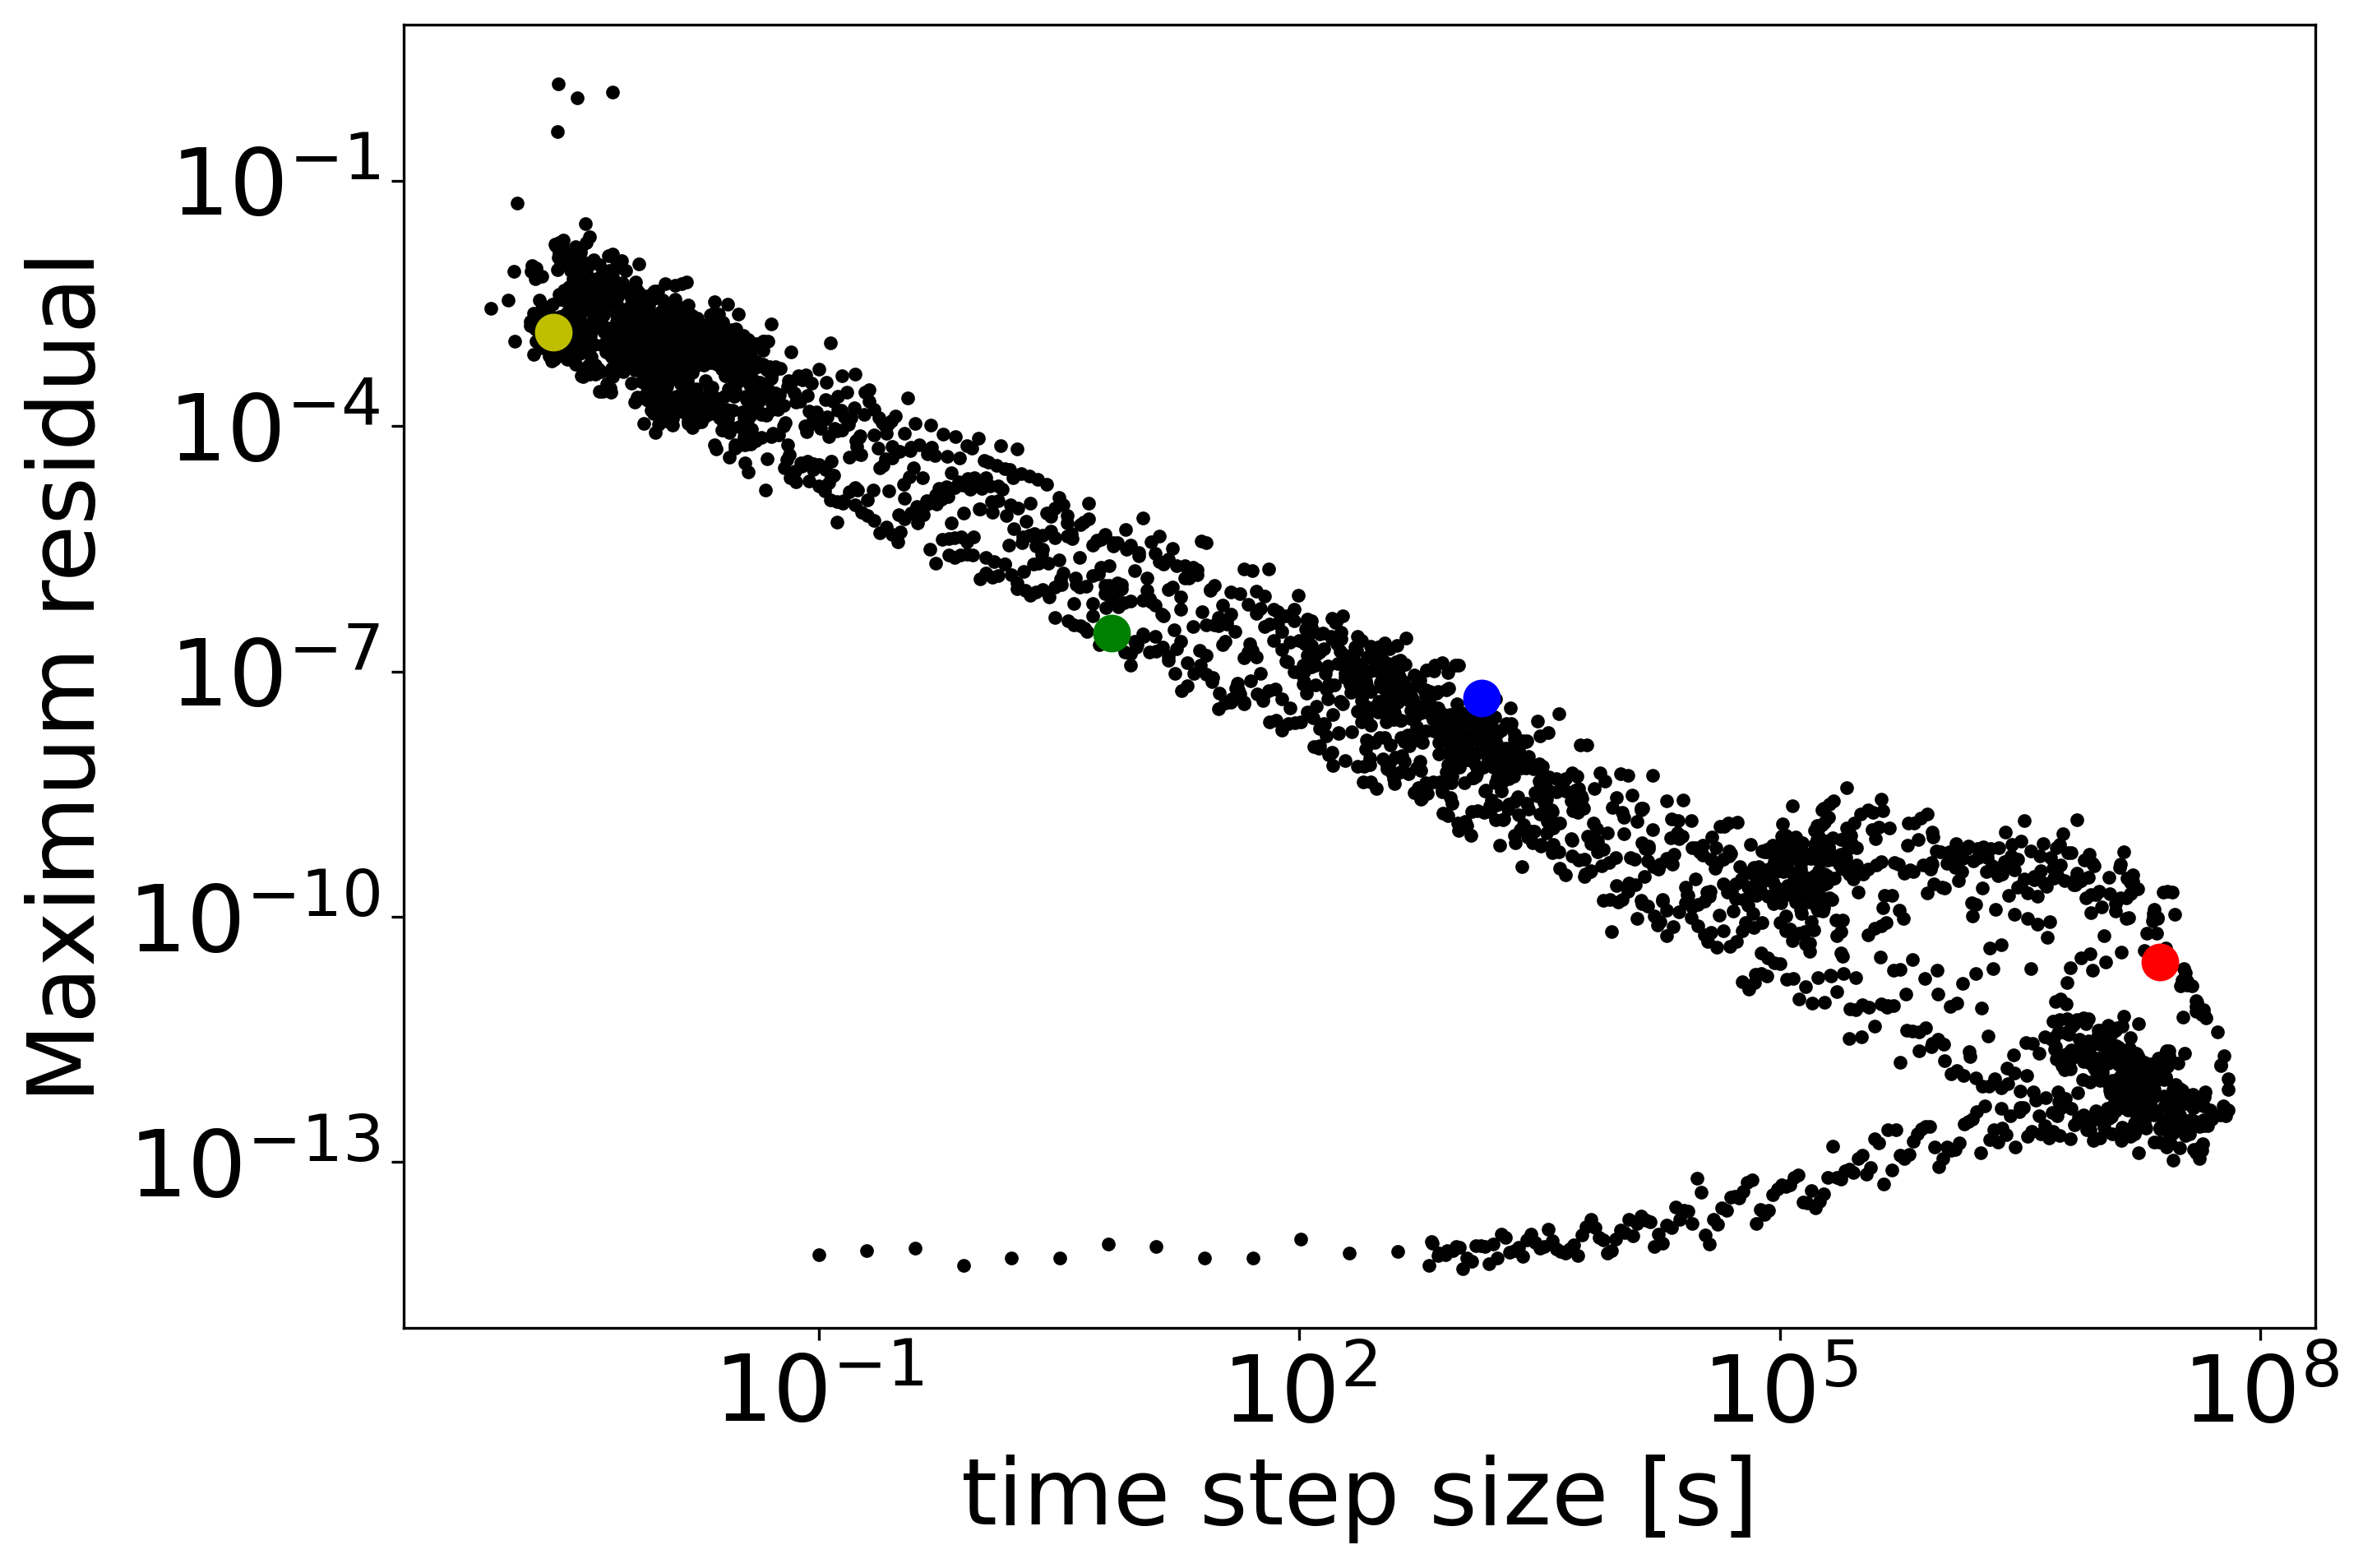
\includegraphics[width=1\textwidth]{images/TANDEMConvergenceAnalysisCompactDAEMaxResidual_Size5.png}
		\subcaption{Minimum achievable residual norms in function of the timestep size}
		\label{fig:convergenceIssuesCompactDAEMaxResidual_vs_dt}
	\end{subfigure}
	\begin{subfigure}[t]{0.32\textwidth}
		\centering
		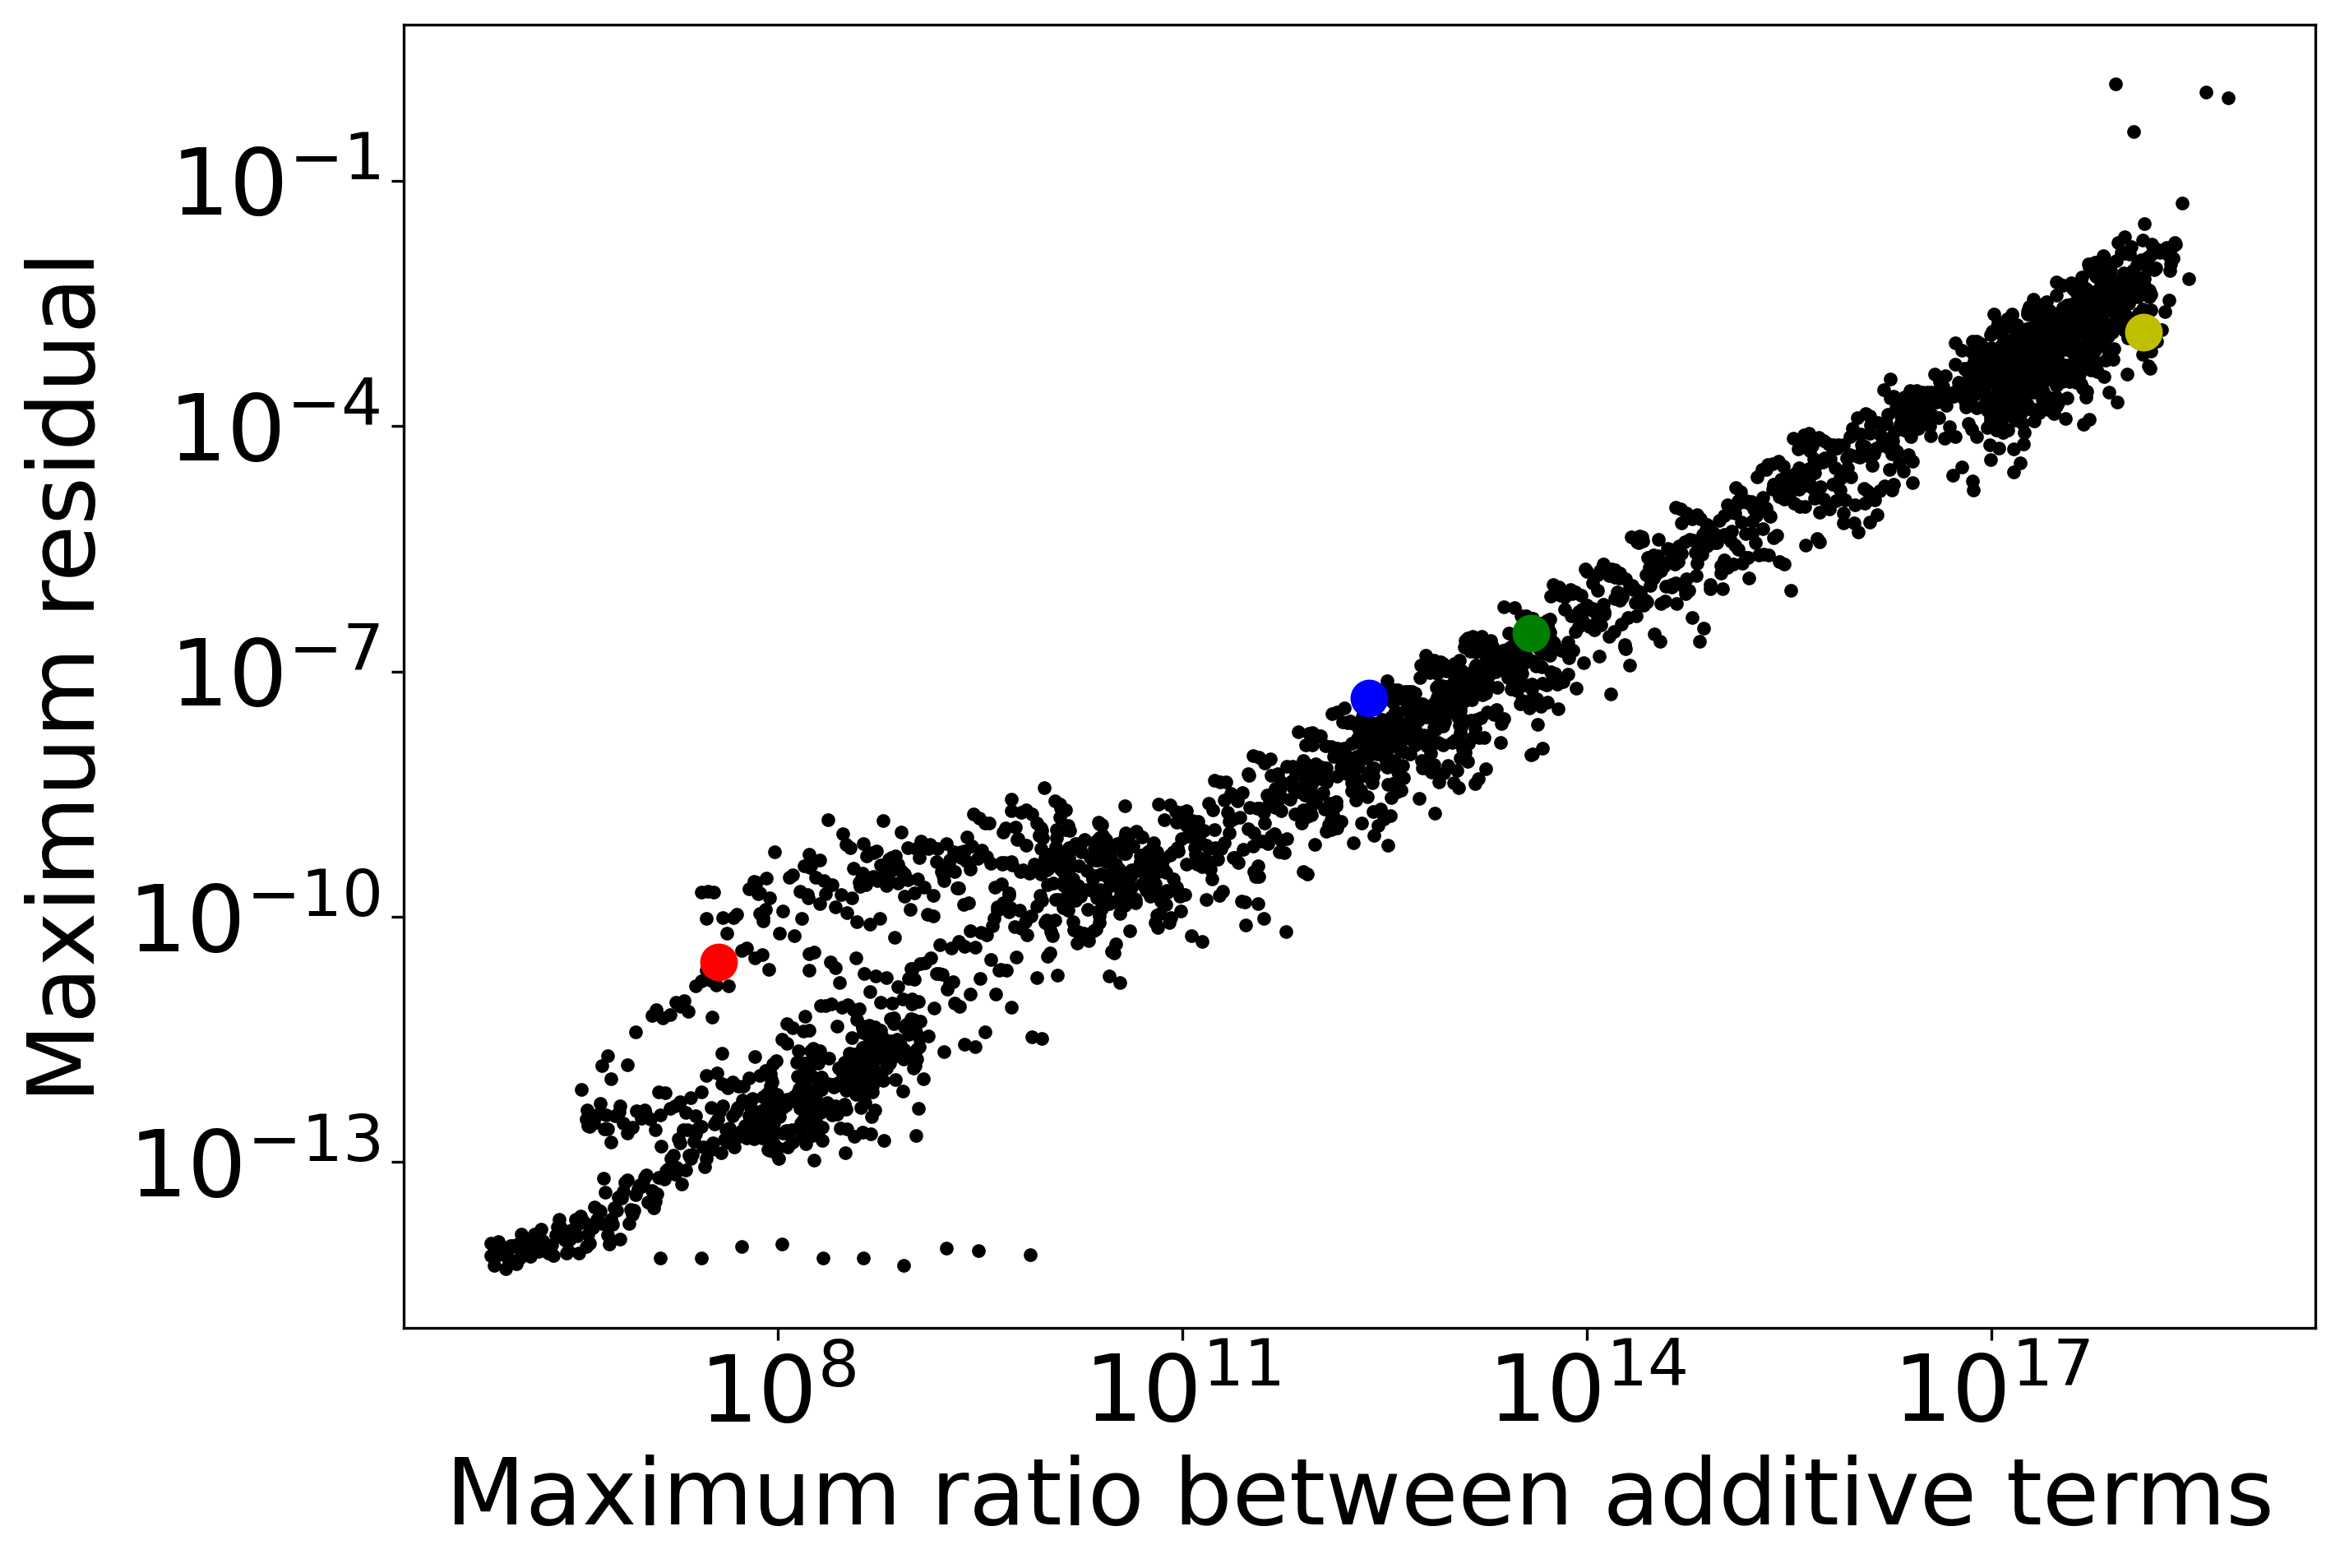
\includegraphics[width=1\textwidth]{images/TANDEMConvergenceAnalysisCompactDAERatioInAddition_Size5.png}
		\subcaption{Minimum achievable residual norms in function of the maximal ratio between the additive terms in the Jacobian matrix} 
		\label{fig:convergenceIssuesCompactDAEMaxResidual_vs_ratio}
	\end{subfigure}
	\caption{Convergence properties of the compact DAE formulation with the 4th order BDF method on a small domain with 5 fault elements}
\end{figure}

The reason for this poor convergence can be found in the definition of the Jacobian matrix of the compact DAE formulation in \autoref{eq:Jacobian_compact_DAE}. As a quick remainder, the Jacobian matrix in the Newton iteration is obtained by $\mathbf{J} = \mathbf{F}_x + \sigma \mathbf{F}_{\dot{x}}$, where the shift $\sigma$ depends on the order $k$ of the BDF scheme and on the timestep sizes in the $k$ previous timesteps. The upper left block in the Jacobian is thus the sum of $\sigma\pdv{f}{V}$ and $\pdv{f}{S}$. The first partial derivative is of the magnitude $10^9$ in the aseismic slip and reaches values up to the order $10^{15}$ in an earthquake. On the other hand, the second summand takes values between $10^0$ and $10^2$. Since the former is a diagonal matrix, the sum only affects the diagonal elements. The timestep does not change by a lot between two time iterations, it can be assumed that they are of the same order of magnitude. The shift $\sigma$ is then of the order $\sigma = \Theta\left(h_n^{-1}\right)$, where $h_n$ is current timestep size. In the aseismic slip, $\sigma$ is thus of the order $10^{-7}$ and can go as high as $10^3$ during an earthquake. In the worst case, two terms of orders $10^{18}$ and $10^0$ have to be summed up, which cannot be represented anymore by a double precision floating point variable. The partial derivative $\pdv{f}{S}$ is therefore neglected in the Jacobian matrix during an earthquake and the friction law cannot be solved accurately anymore.
\autoref{fig:convergenceIssuesCompactDAEMaxResidual_vs_ratio} shows the maximum residual at the end of the Newton iteration in function of the ratio $\sigma\pdv{f}{V} / \pdv{f}{S}$ between the two problematic summands. As the ratio approaches and surpasses the machine precision of approximately $10^{16}$, the minimal achievable residual norm also increases. As a matter of fact, the bad accuracy only appears in the residual components in $S$, for which the problematic summation occurs, whereas the residual components in $\psi$ remain at very good values below $10^{-12}$ throughout the simulation.
\\
In the last two graphs, a band with high accuracy and low timestep size appears at the bottom. These points correspond to the initial phase of the simulation, which is always launched in the aseismic slip phase with $h_0=0.1s$. Since the solution vector contains the initial value in these points, the Newton iteration converges directly with a high precision. \\
This issue occurs only with the compact DAE formulation, because the Jacobian matrices of the ODE formulations do not require any summations and in the extended DAE formulation, the two problematic terms $\pdv{f}{V}$ and $\pdv{f}{S}$ are located in different submatrices of $\mathbf{F}_{\dot{x}}$ and $\mathbf{F}_x$ and are thus never added to each other. \autoref{fig:convergenceIssuesExtendedDAEMaxResidual_vs_dt} shows the same dependency as in \autoref{fig:convergenceIssuesCompactDAEMaxResidual_vs_dt} for the extended DAE formulation. The norm of the residual at the end of the Newton iteration here does not depend on the timestep size and it varies between $10^{-12}$ and $10^{-15}$ throughout the simulation. Since both the slip and the state variable are of the order of $10^0$, the achieved tolerance is excellent and close to machine precision. However, it seems that the best accuracy is only reached for large timesteps, whereas for very small timesteps, the Newton iteration only reached the "not the best but still very good" - accuracy of $10^{-12}$. In the definition of the Jacobian matrix for the extended DAE formulation in \autoref{eq:Jacobian_Newton_Iteration_extended_DAE}, there still is an addition between the shift $\sigma$ ($\sigma=1/h$ in the referred equation because it is related to the implicit Euler method) and the term $\pdv{g}{\psi}$. Since this last term is always of the order $10^{-7}$, the difference between the summands is not as extreme as for the compact formulation, but still noticeable for small time steps, where $\sigma \approx 10^3$. Looking at \autoref{fig:convergenceIssuesExtendedDAEMaxResidual_vs_dt_onlyPSI}, the components of the residual vector relative to $\psi$ increase if the timestep size decreases. This is the same behavior as previously, but on a much lower magnitude. Only in the earthquake phase, when timesteps below $0.1s$ are encountered, the residual in $\psi$ exceed the maximal precision $10^{-15}$ of the friction law and impacts the overall accuracy. 

\begin{figure}[H]
	\centering
	\begin{subfigure}[t]{0.45\textwidth}
	\centering
		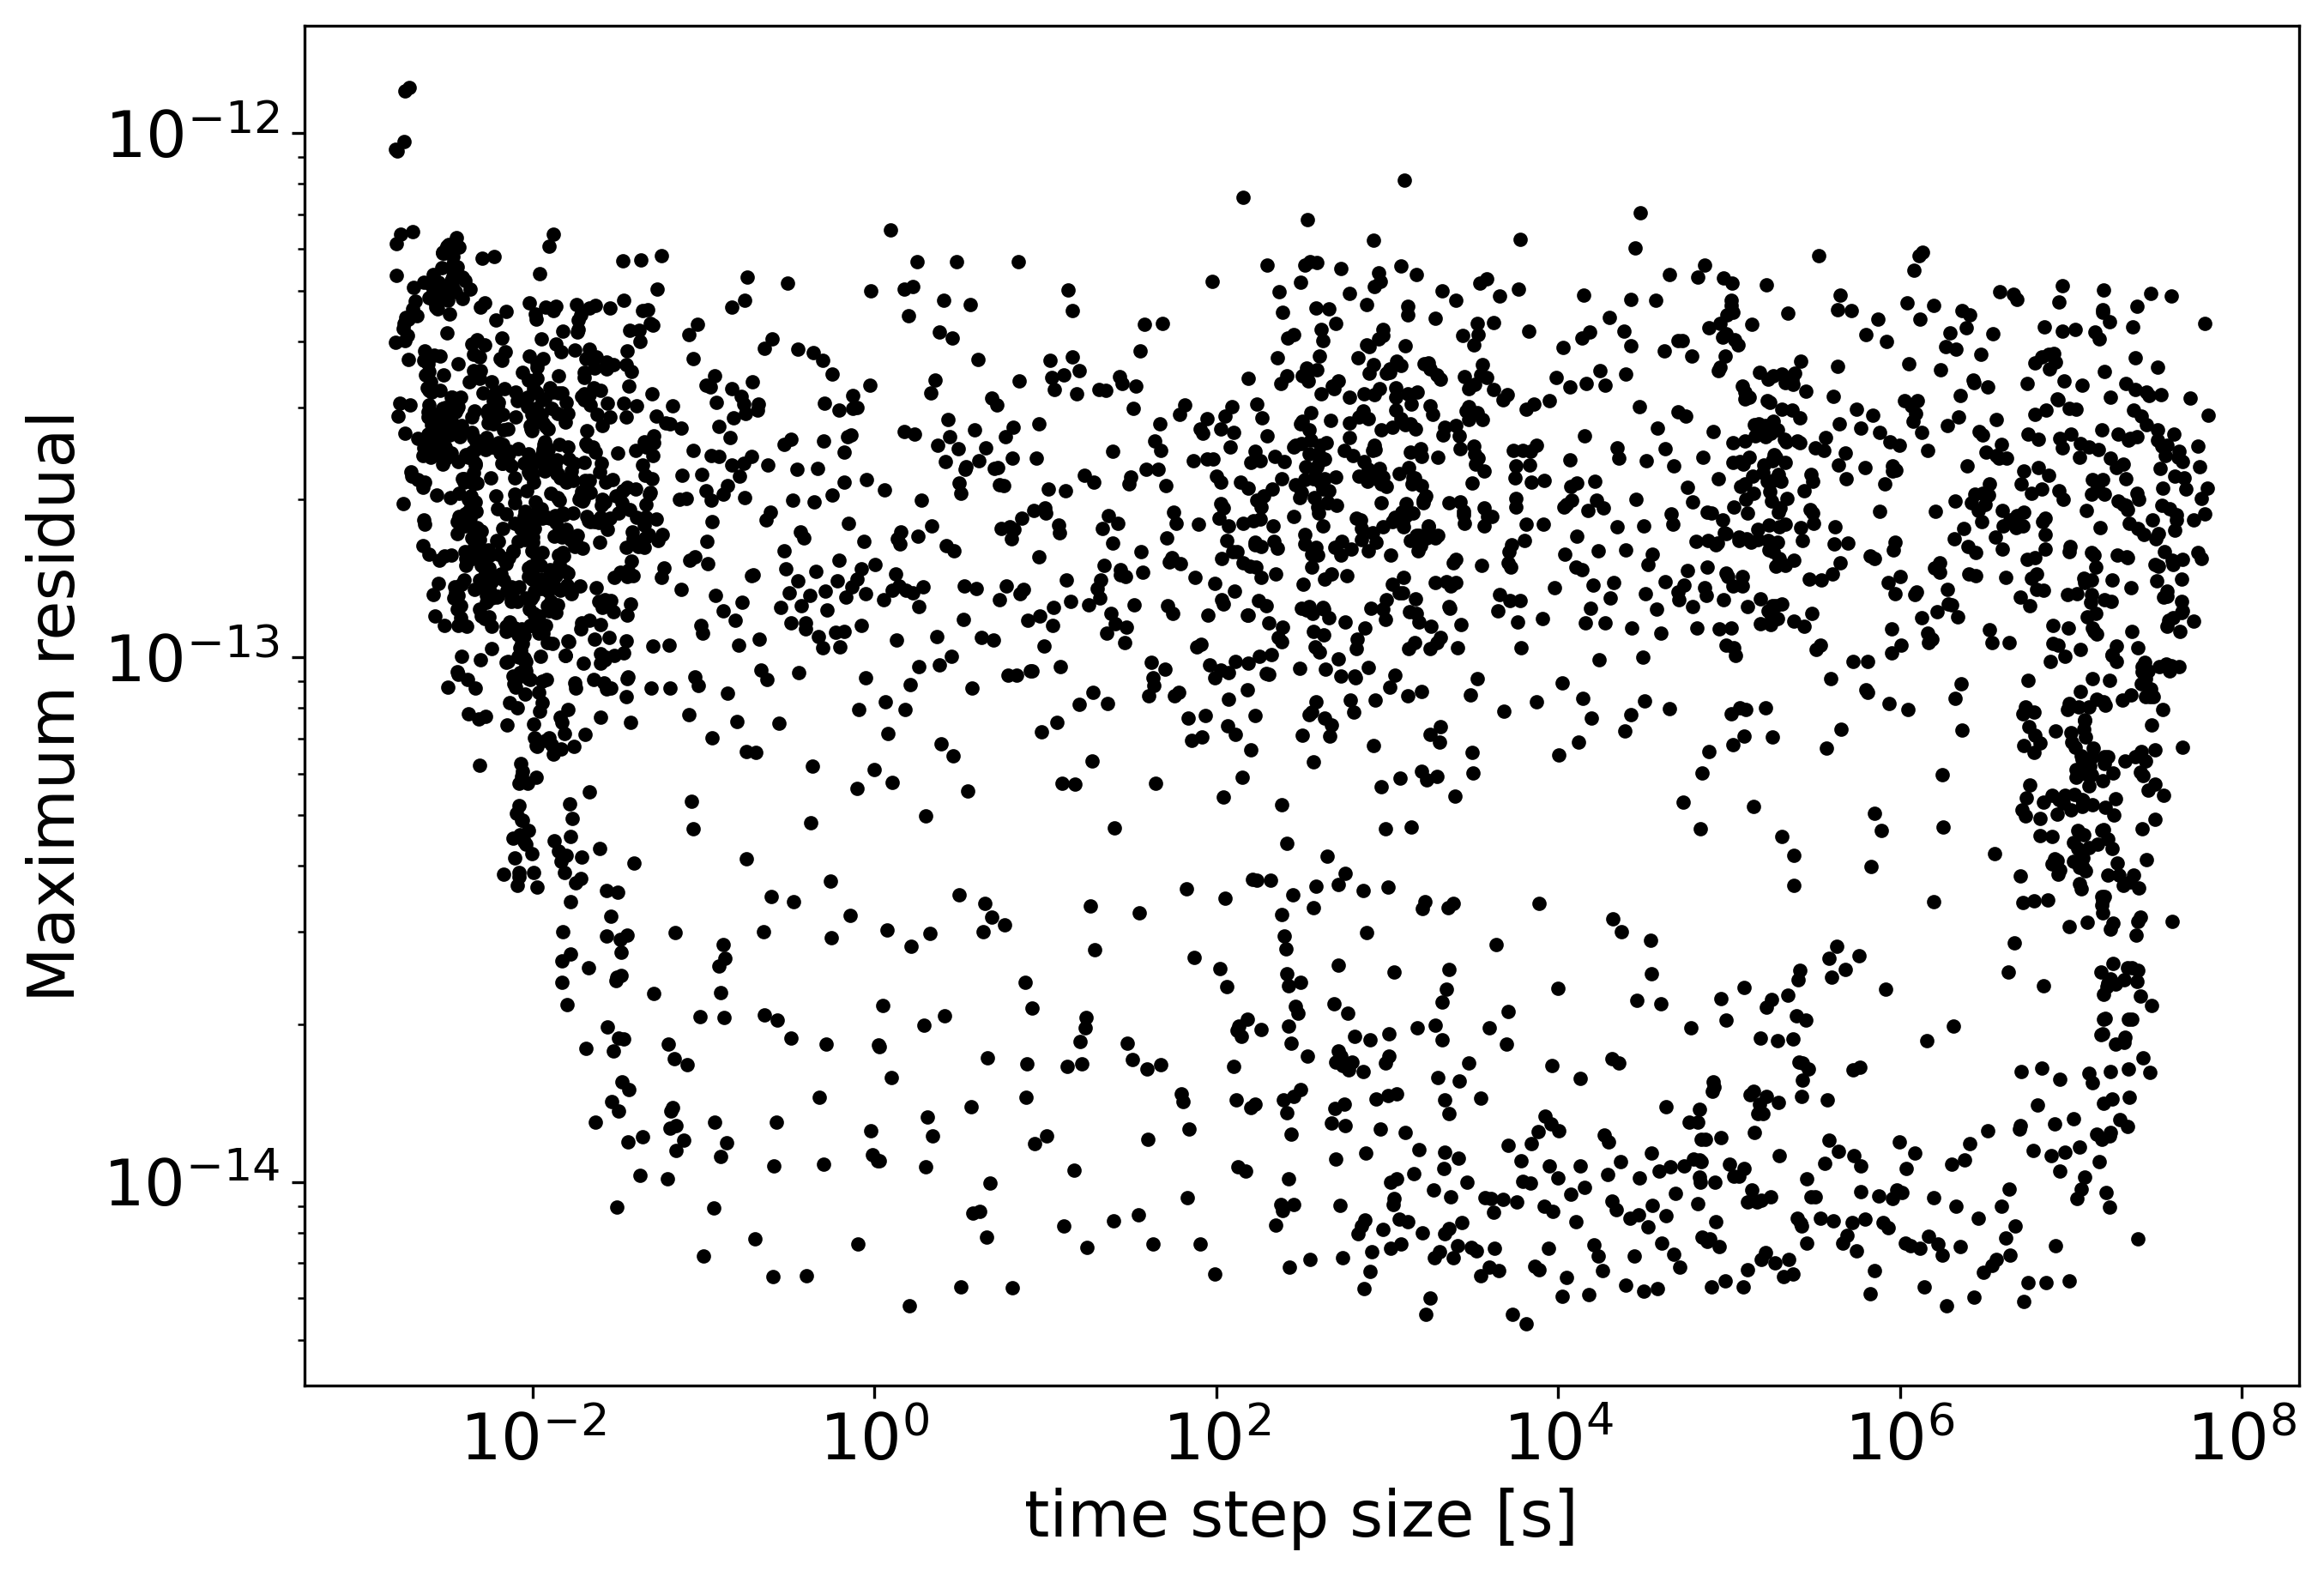
\includegraphics[width=1\textwidth]{images/TANDEMConvergenceAnalysisExtendedDAEMaxResidual_Size5.png}
		\caption{Residual of all components}
		\label{fig:convergenceIssuesExtendedDAEMaxResidual_vs_dt}
	\end{subfigure} 
	\begin{subfigure}[t]{0.45\textwidth}
		\centering
		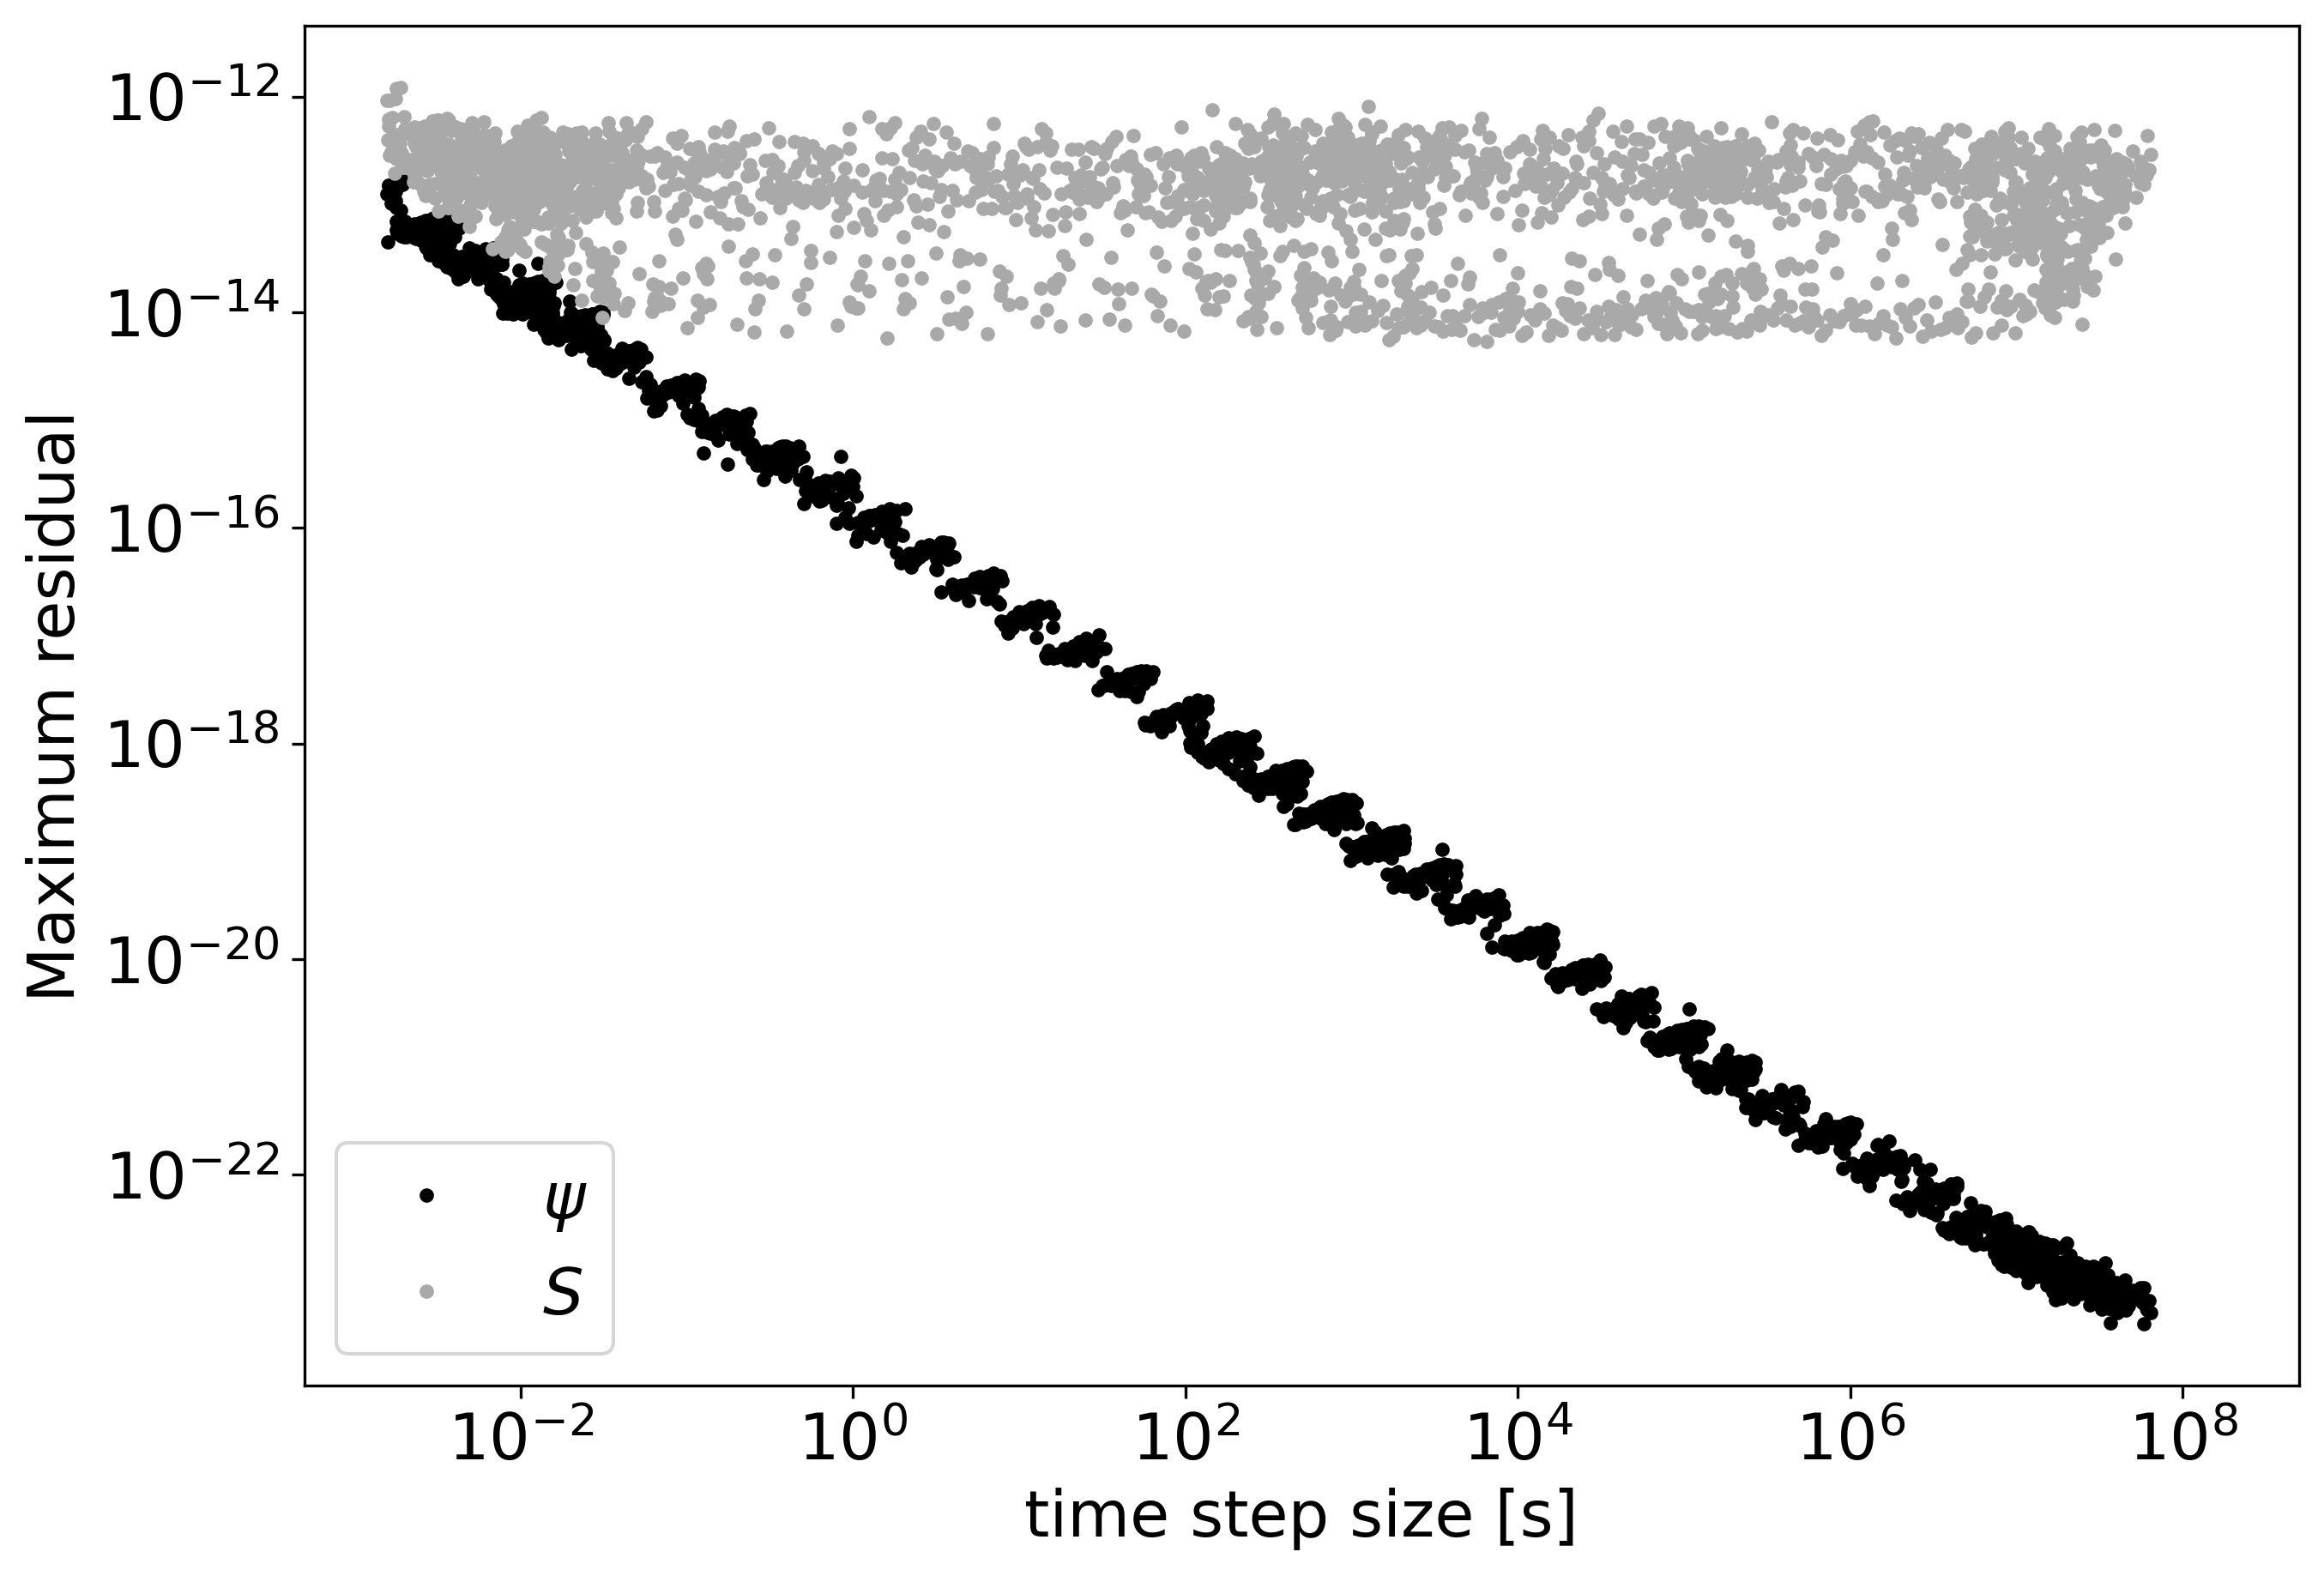
\includegraphics[width=1\textwidth]{images/TANDEMConvergenceAnalysisExtendedDAEMaxResidual_Size5_onlyPSI.png}
		\caption{Residual of the individual components $\psi$ and $S$}
		\label{fig:convergenceIssuesExtendedDAEMaxResidual_vs_dt_onlyPSI}
	\end{subfigure} 
	\caption{Minimum achievable residual norms in function of the timestep size for the extended DAE formulation with the 4th order BDF method on a small domain with 5 fault elements}
\end{figure}

\begin{figure}[H]
\end{figure}

In conclusion, the compact DAE formulation fails for the earthquake and can only be applied in the aseismic slip phase. Since the accuracy decreases along with the timestep size, the usual strategy to restart a step with a smaller timestep size if the nonlinear did not converge only leads to an even worse accuracy and is unsuitable. For this limited purpose, it still offers advantages over other methods which will be discussed in a further section.

\subsection{Data structure}
\subsubsection{Block structure}
\subsubsection{Memory requirements}

\section{Results}
\subsection{Comparison between the different formulations of problem}
The simulation is run over a period of 250 years, in which one earthquake occurs on June 13th of the 195th year. This event can be clearly observed in \autoref{fig:timeEvolutionTANDEM_V} which depicts the maximum slip rate over time, which reaches $4.6m\cdot s^{-1}$ as opposed to an average of $1.0 \cdot 10^{-9}m\cdot s^{-1}$ in calm times. 
\begin{figure}[H]
    \centering
    \begin{subfigure}{0.32\textwidth}
     	\centering
    	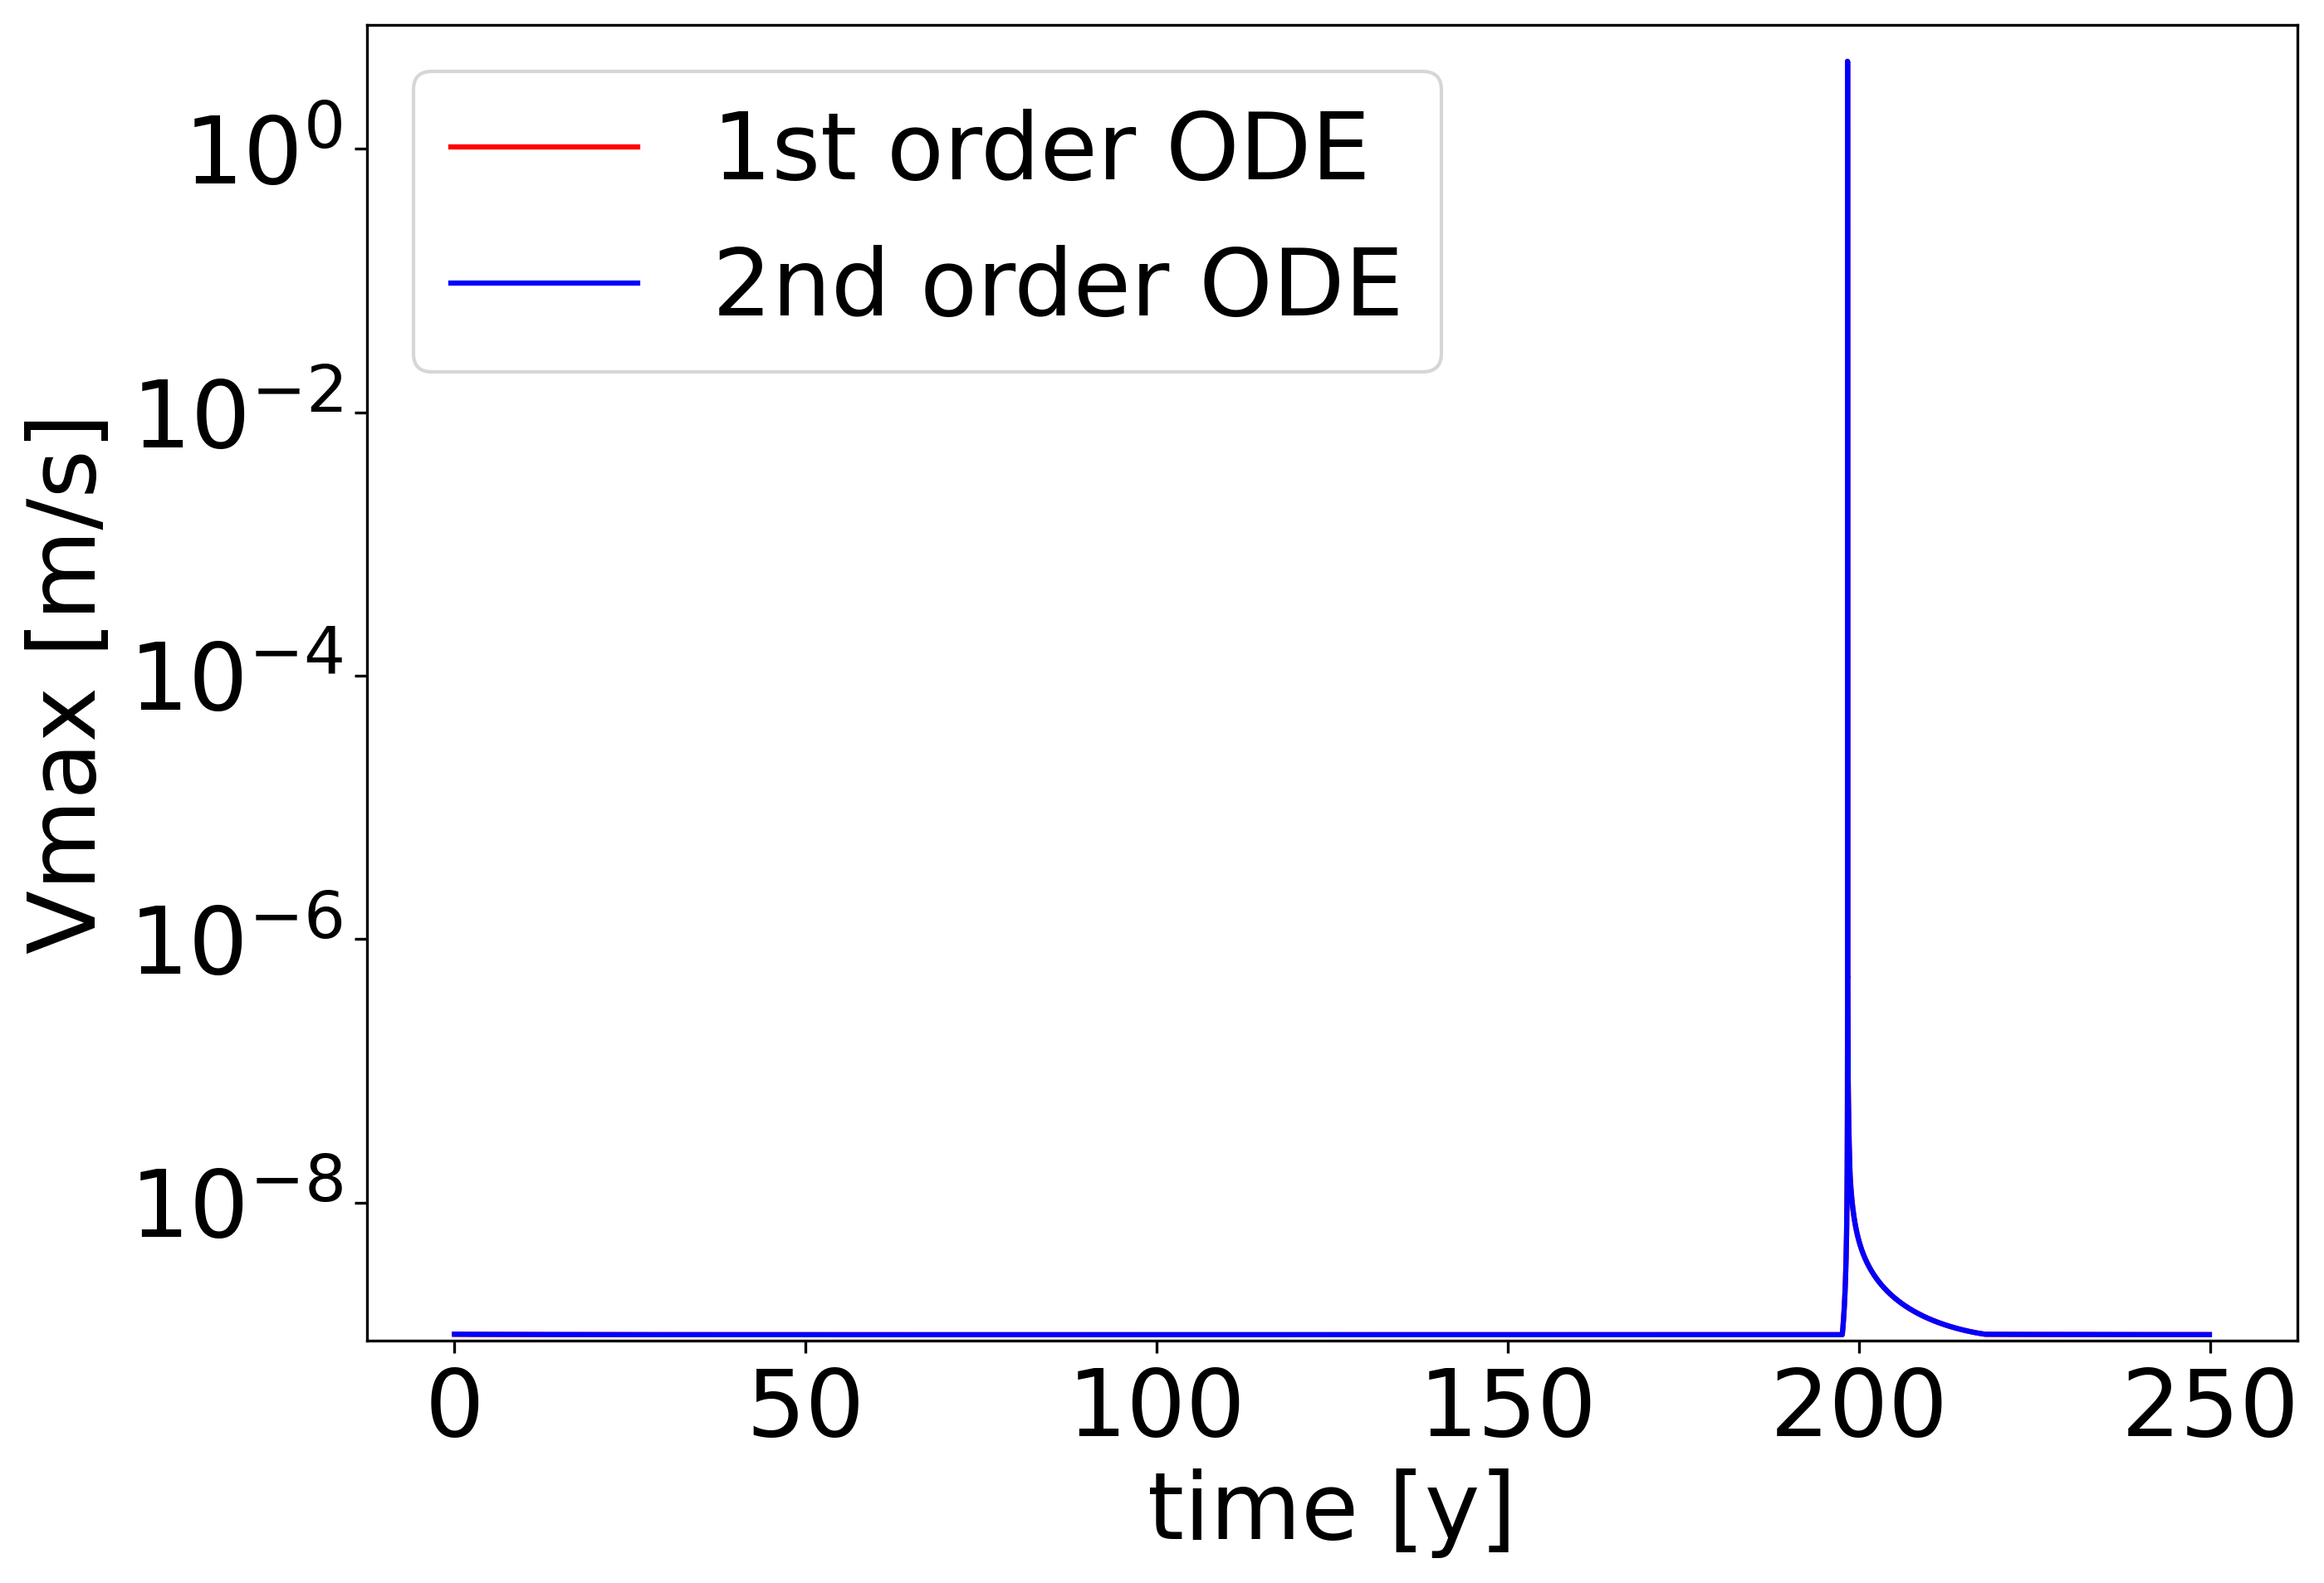
\includegraphics[width=1\textwidth]{images/TANDEMcompareFormulationstimeEvolutionVall.png}
       	\subcaption{Full simulation time} 
    \end{subfigure} 
    \begin{subfigure}{0.32\textwidth}
    	\centering
    	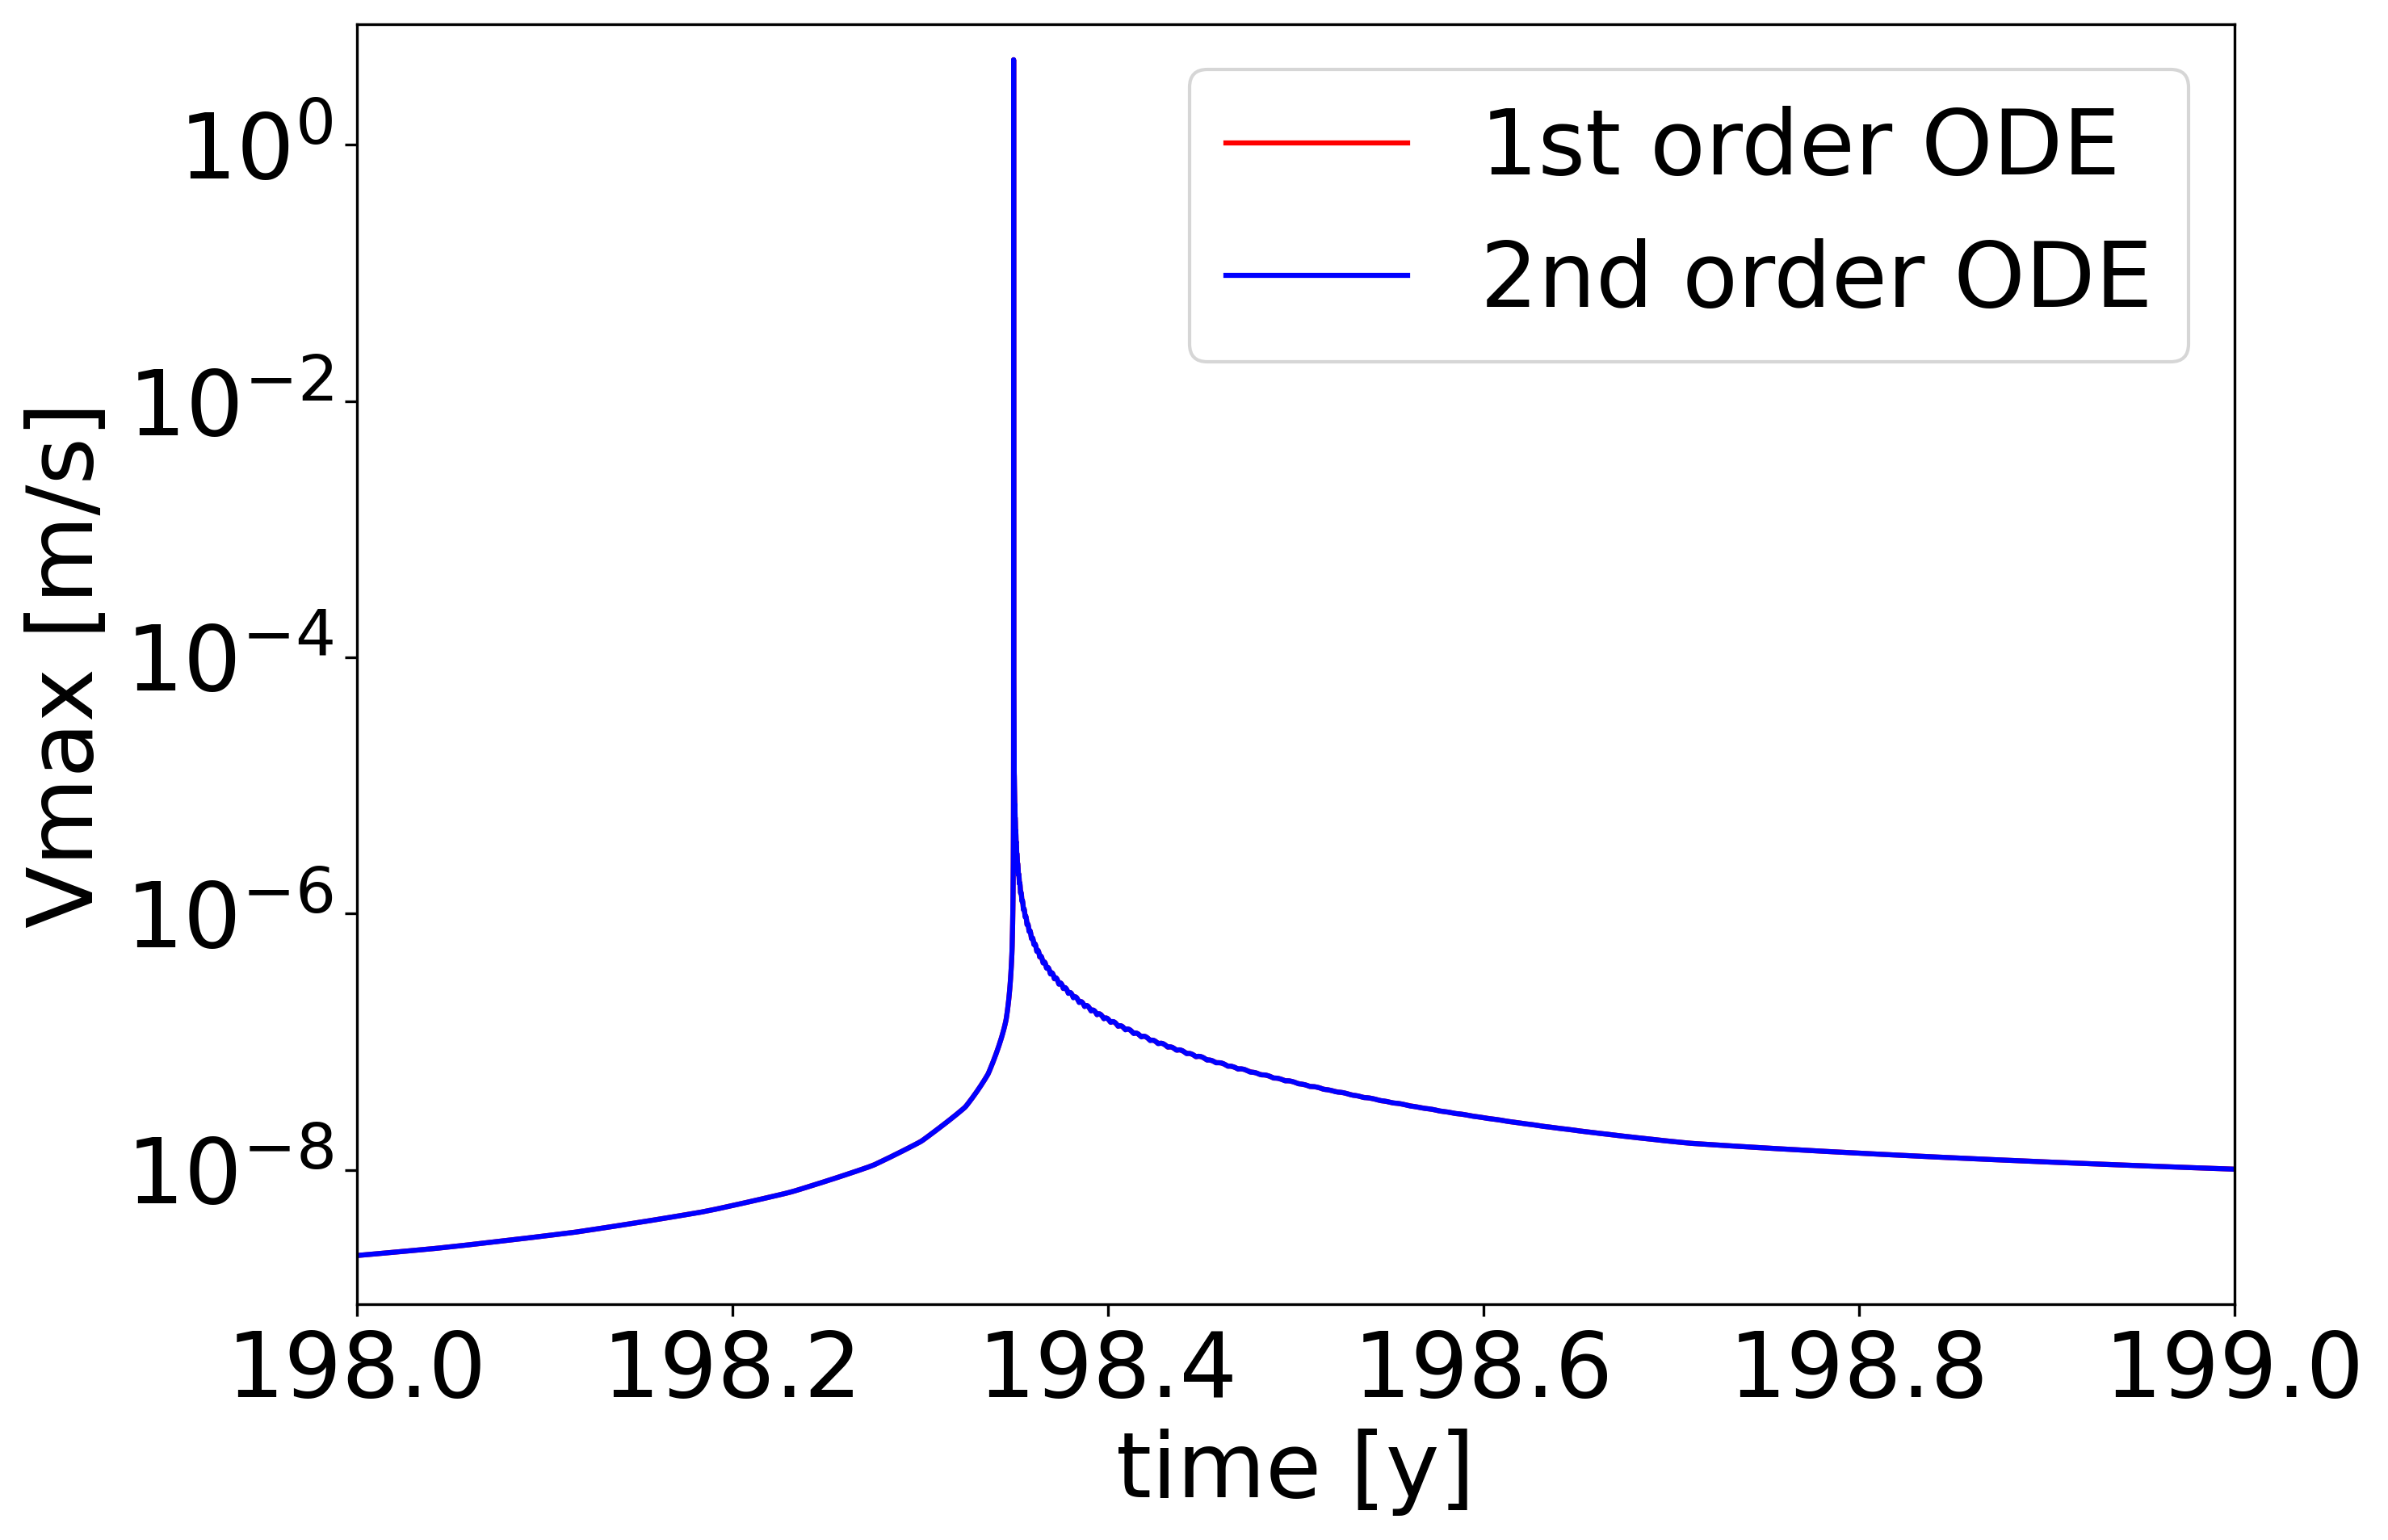
\includegraphics[width=1\textwidth]{images/TANDEMcompareFormulationstimeEvolutionVsurroundings.png}
       	\subcaption{Year of the earthquake} 
    \end{subfigure}
    \begin{subfigure}{0.32\textwidth}
    	\centering
    	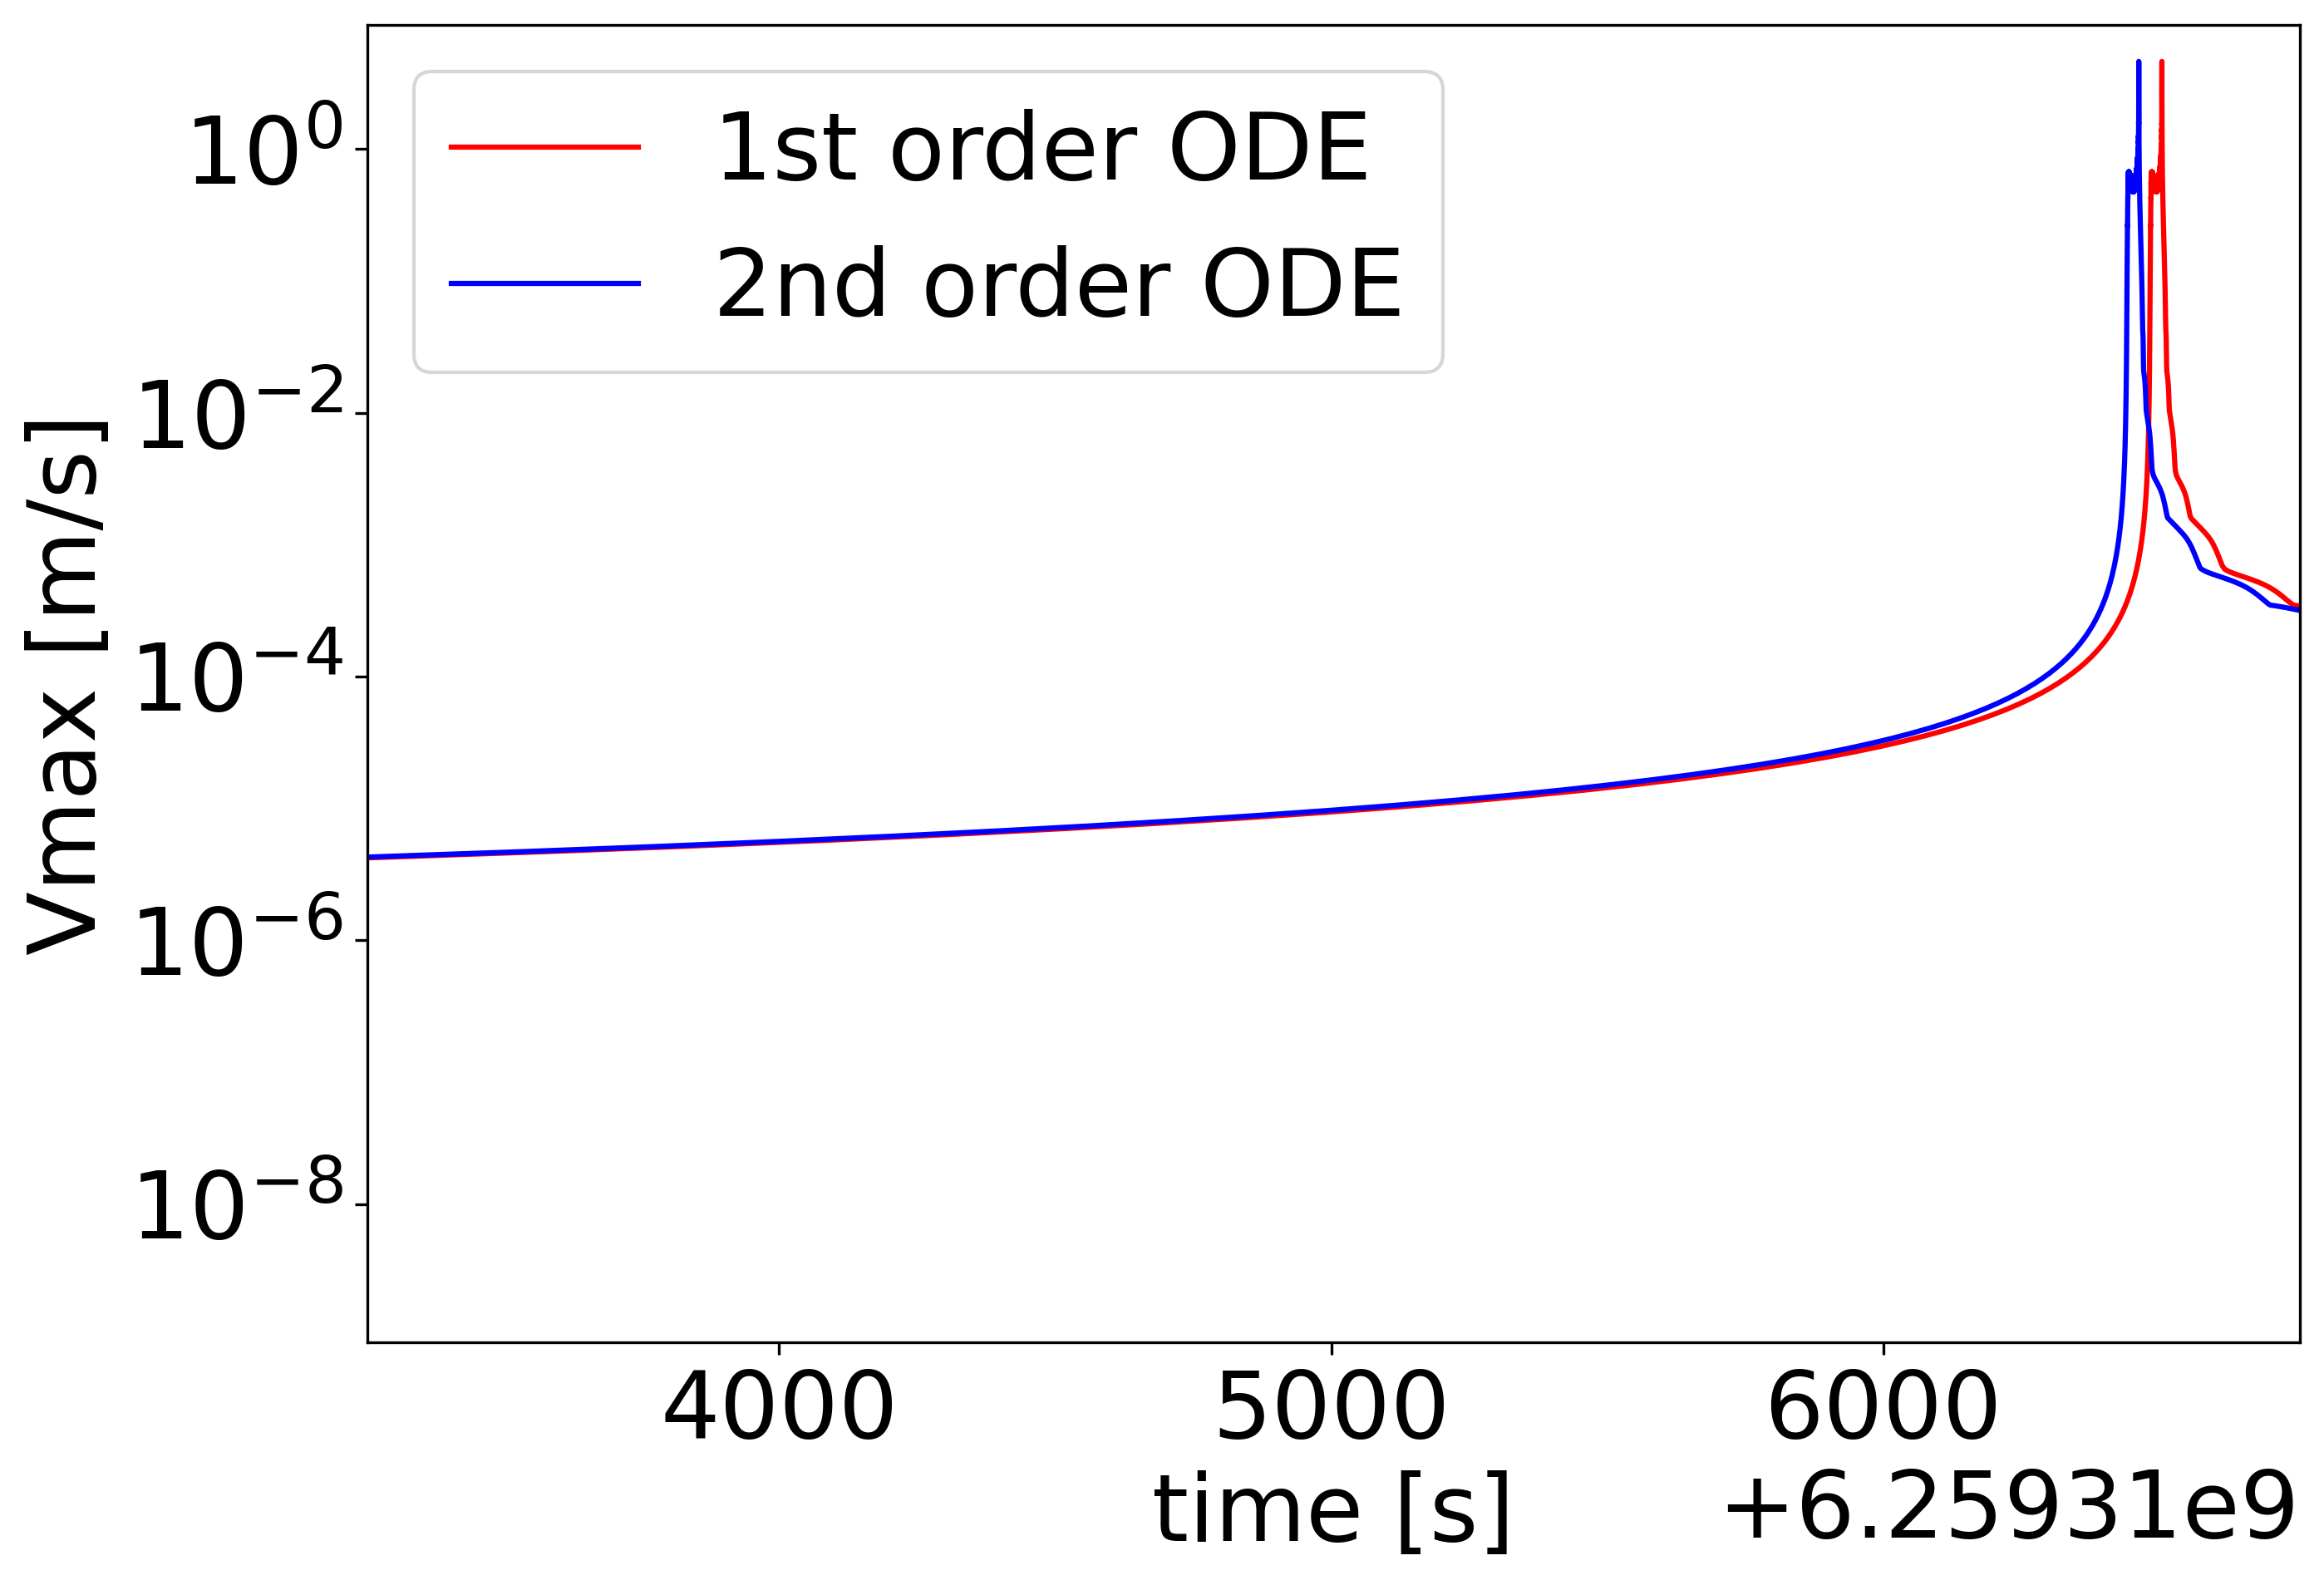
\includegraphics[width=1\textwidth]{images/TANDEMcompareFormulationstimeEvolutionVearthquake.png}
       	\subcaption{Evolution of the earthquake event} 
    \end{subfigure}
    \caption{Evolution of the maximal slip rate $V$ on the fault for different solvers on the symmetric two-dimensional BP1 problem with 200 elements on the fault}
    \label{fig:timeEvolutionTANDEM_V}
\end{figure}


\begin{figure}[H]
    \centering
    \begin{subfigure}{0.32\textwidth}
    	\centering
    	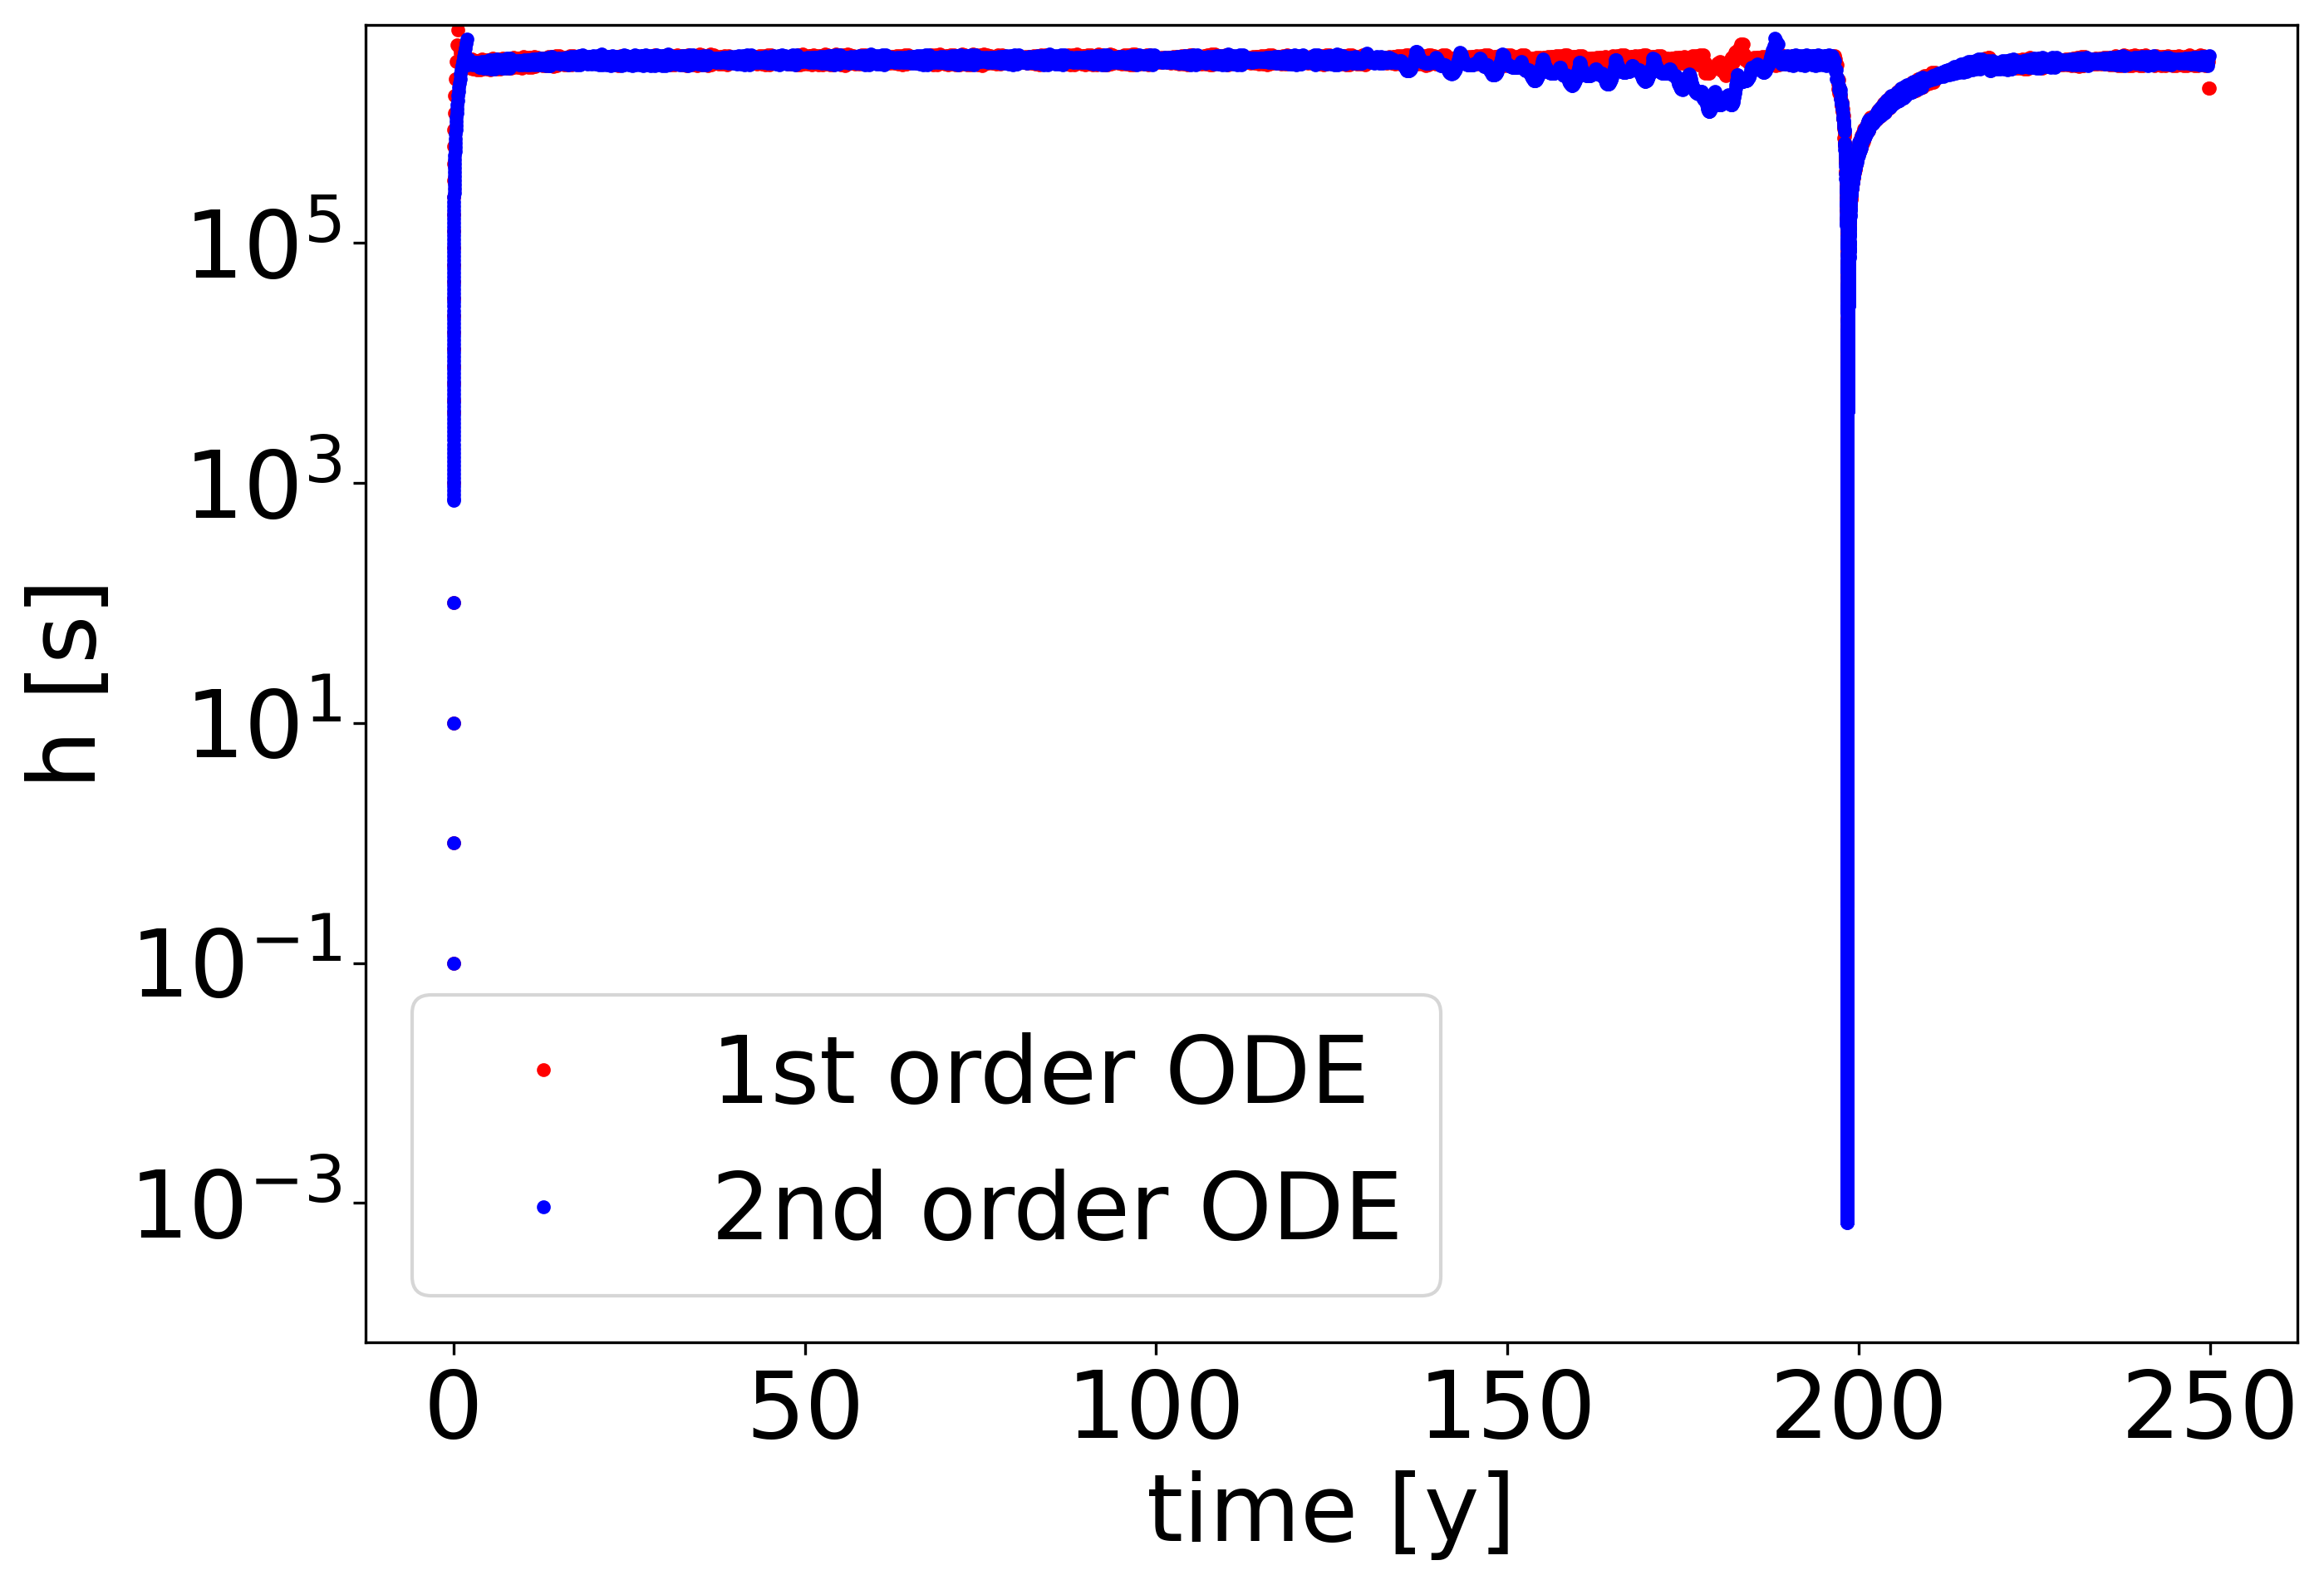
\includegraphics[width=1\textwidth]{images/TANDEMcompareFormulationstimeEvolutionDTall.png}
       	\subcaption{Full simulation time} 
    \end{subfigure}
    \begin{subfigure}{0.32\textwidth}
    	\centering
    	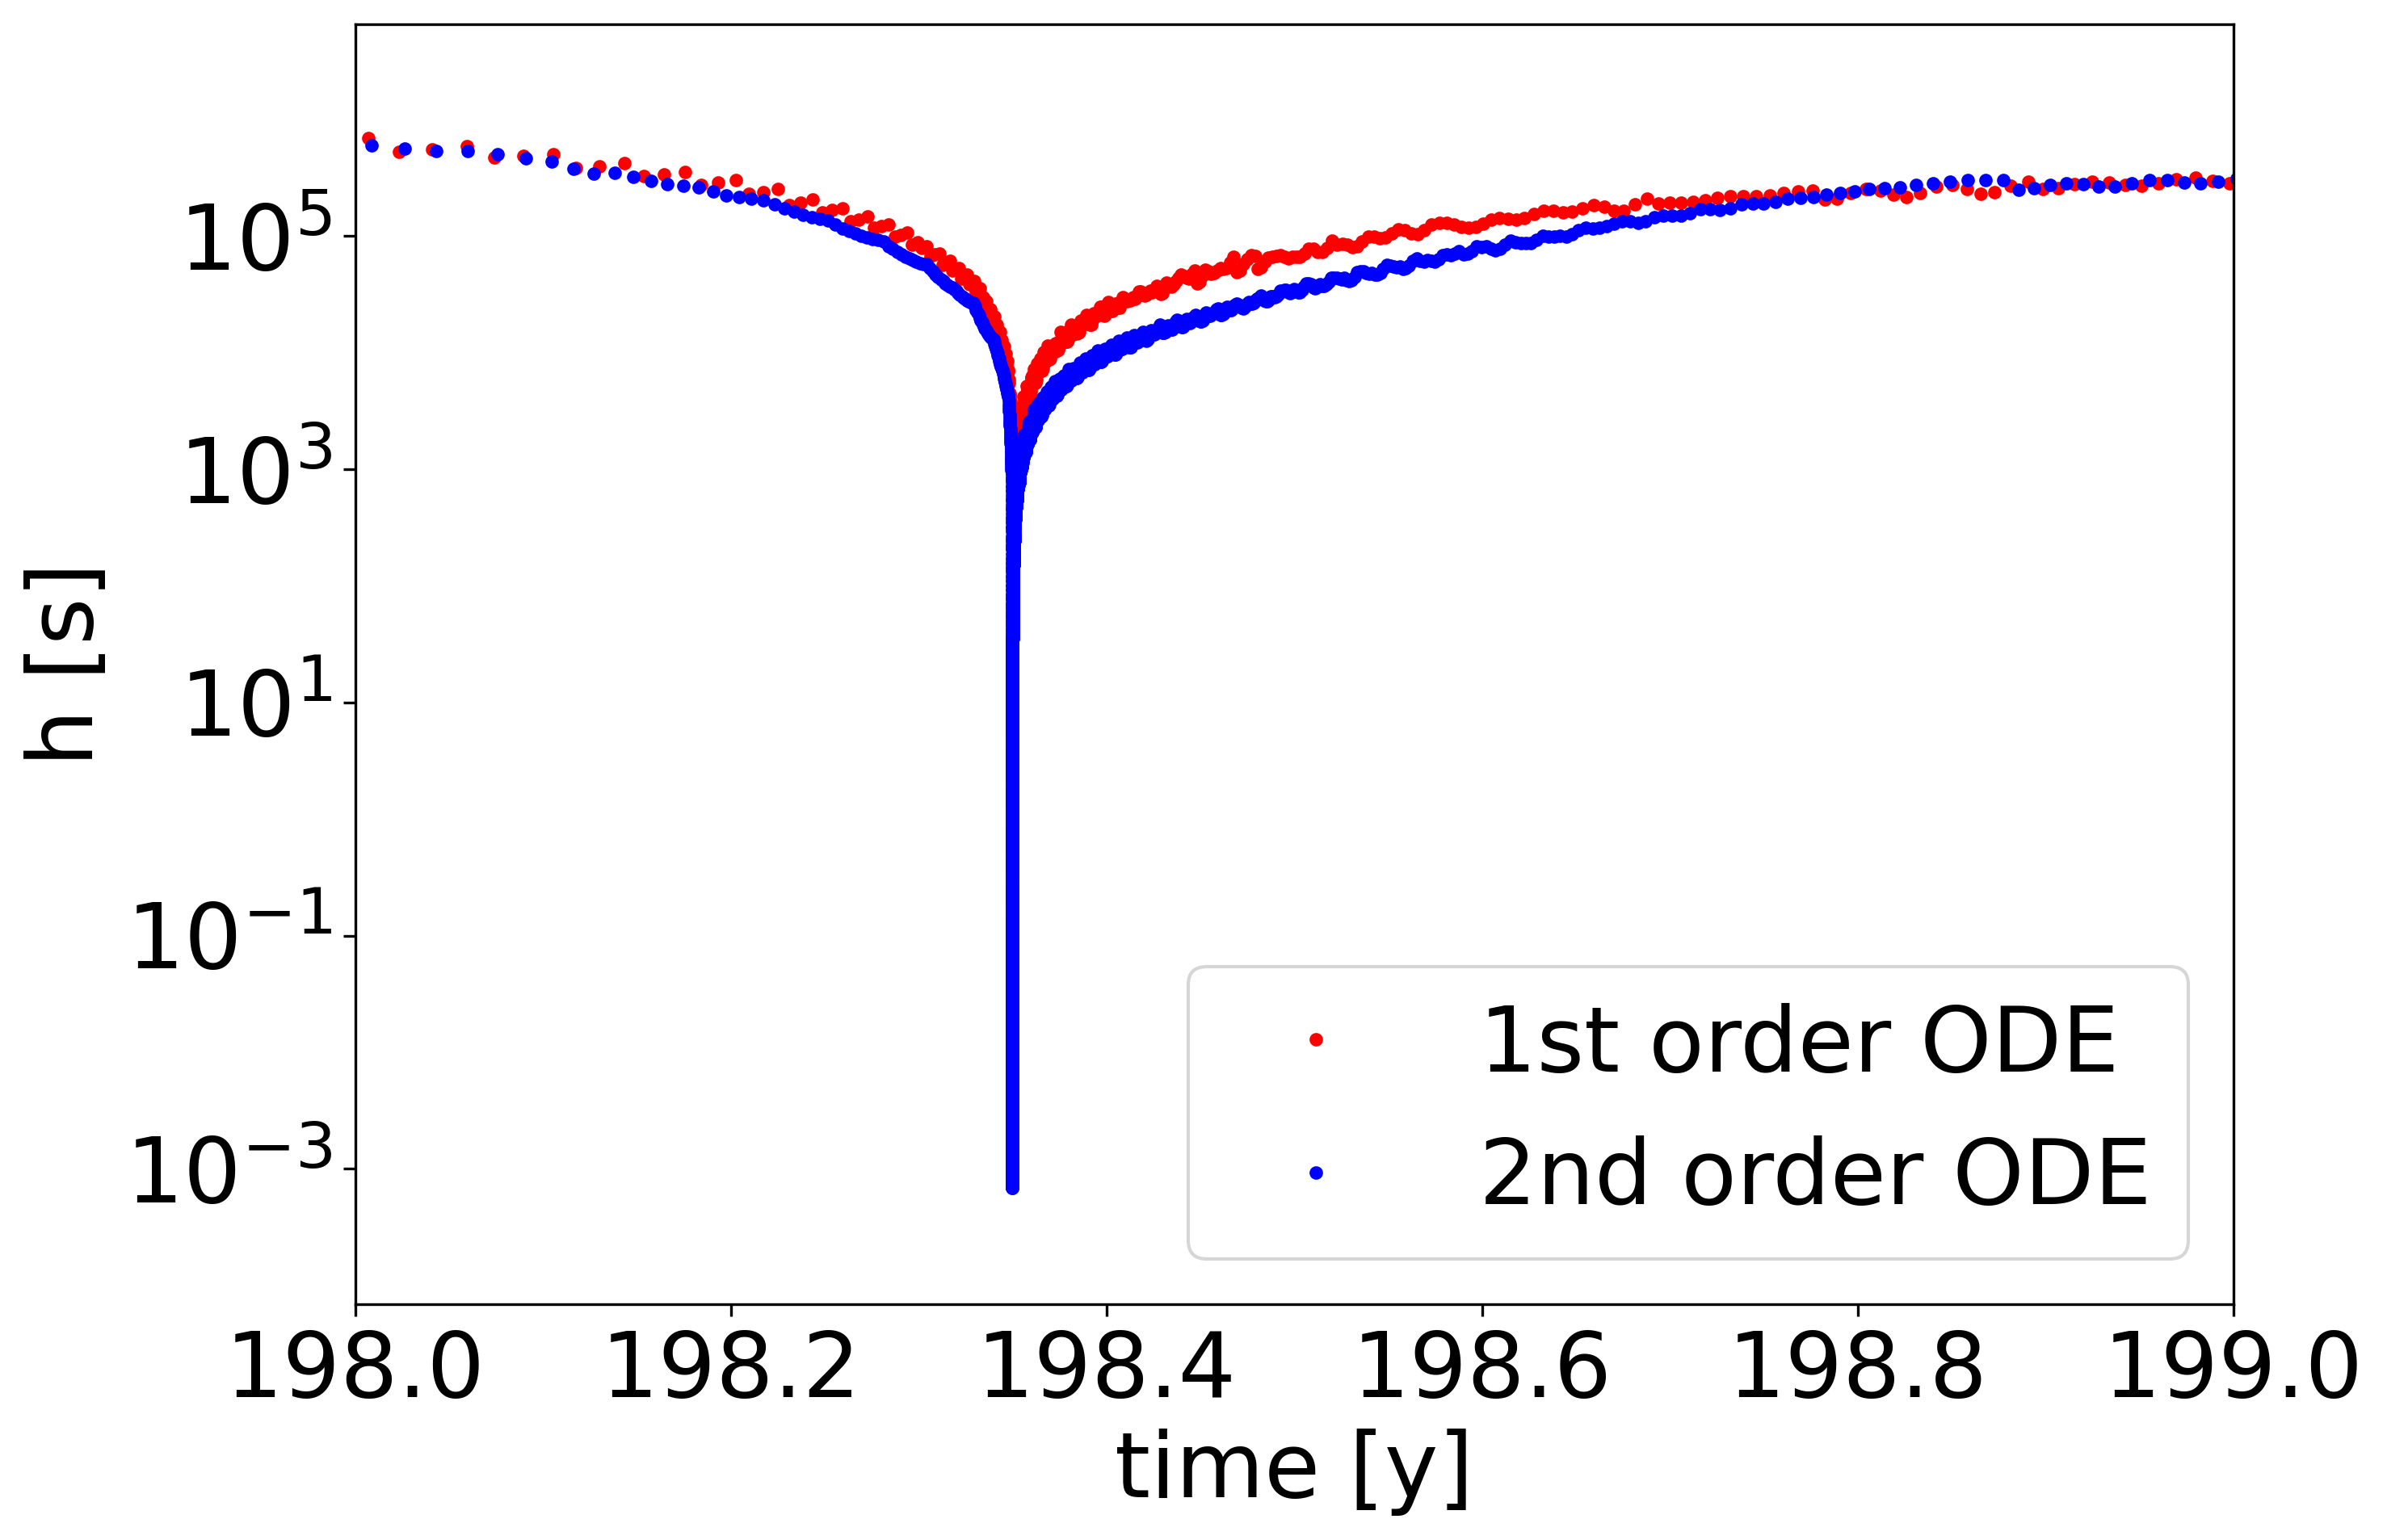
\includegraphics[width=1\textwidth]{images/TANDEMcompareFormulationstimeEvolutionDTsurroundings.png}
       	\subcaption{Year of the earthquake} 
    \end{subfigure}
    \begin{subfigure}{0.32\textwidth}
    	\centering
    	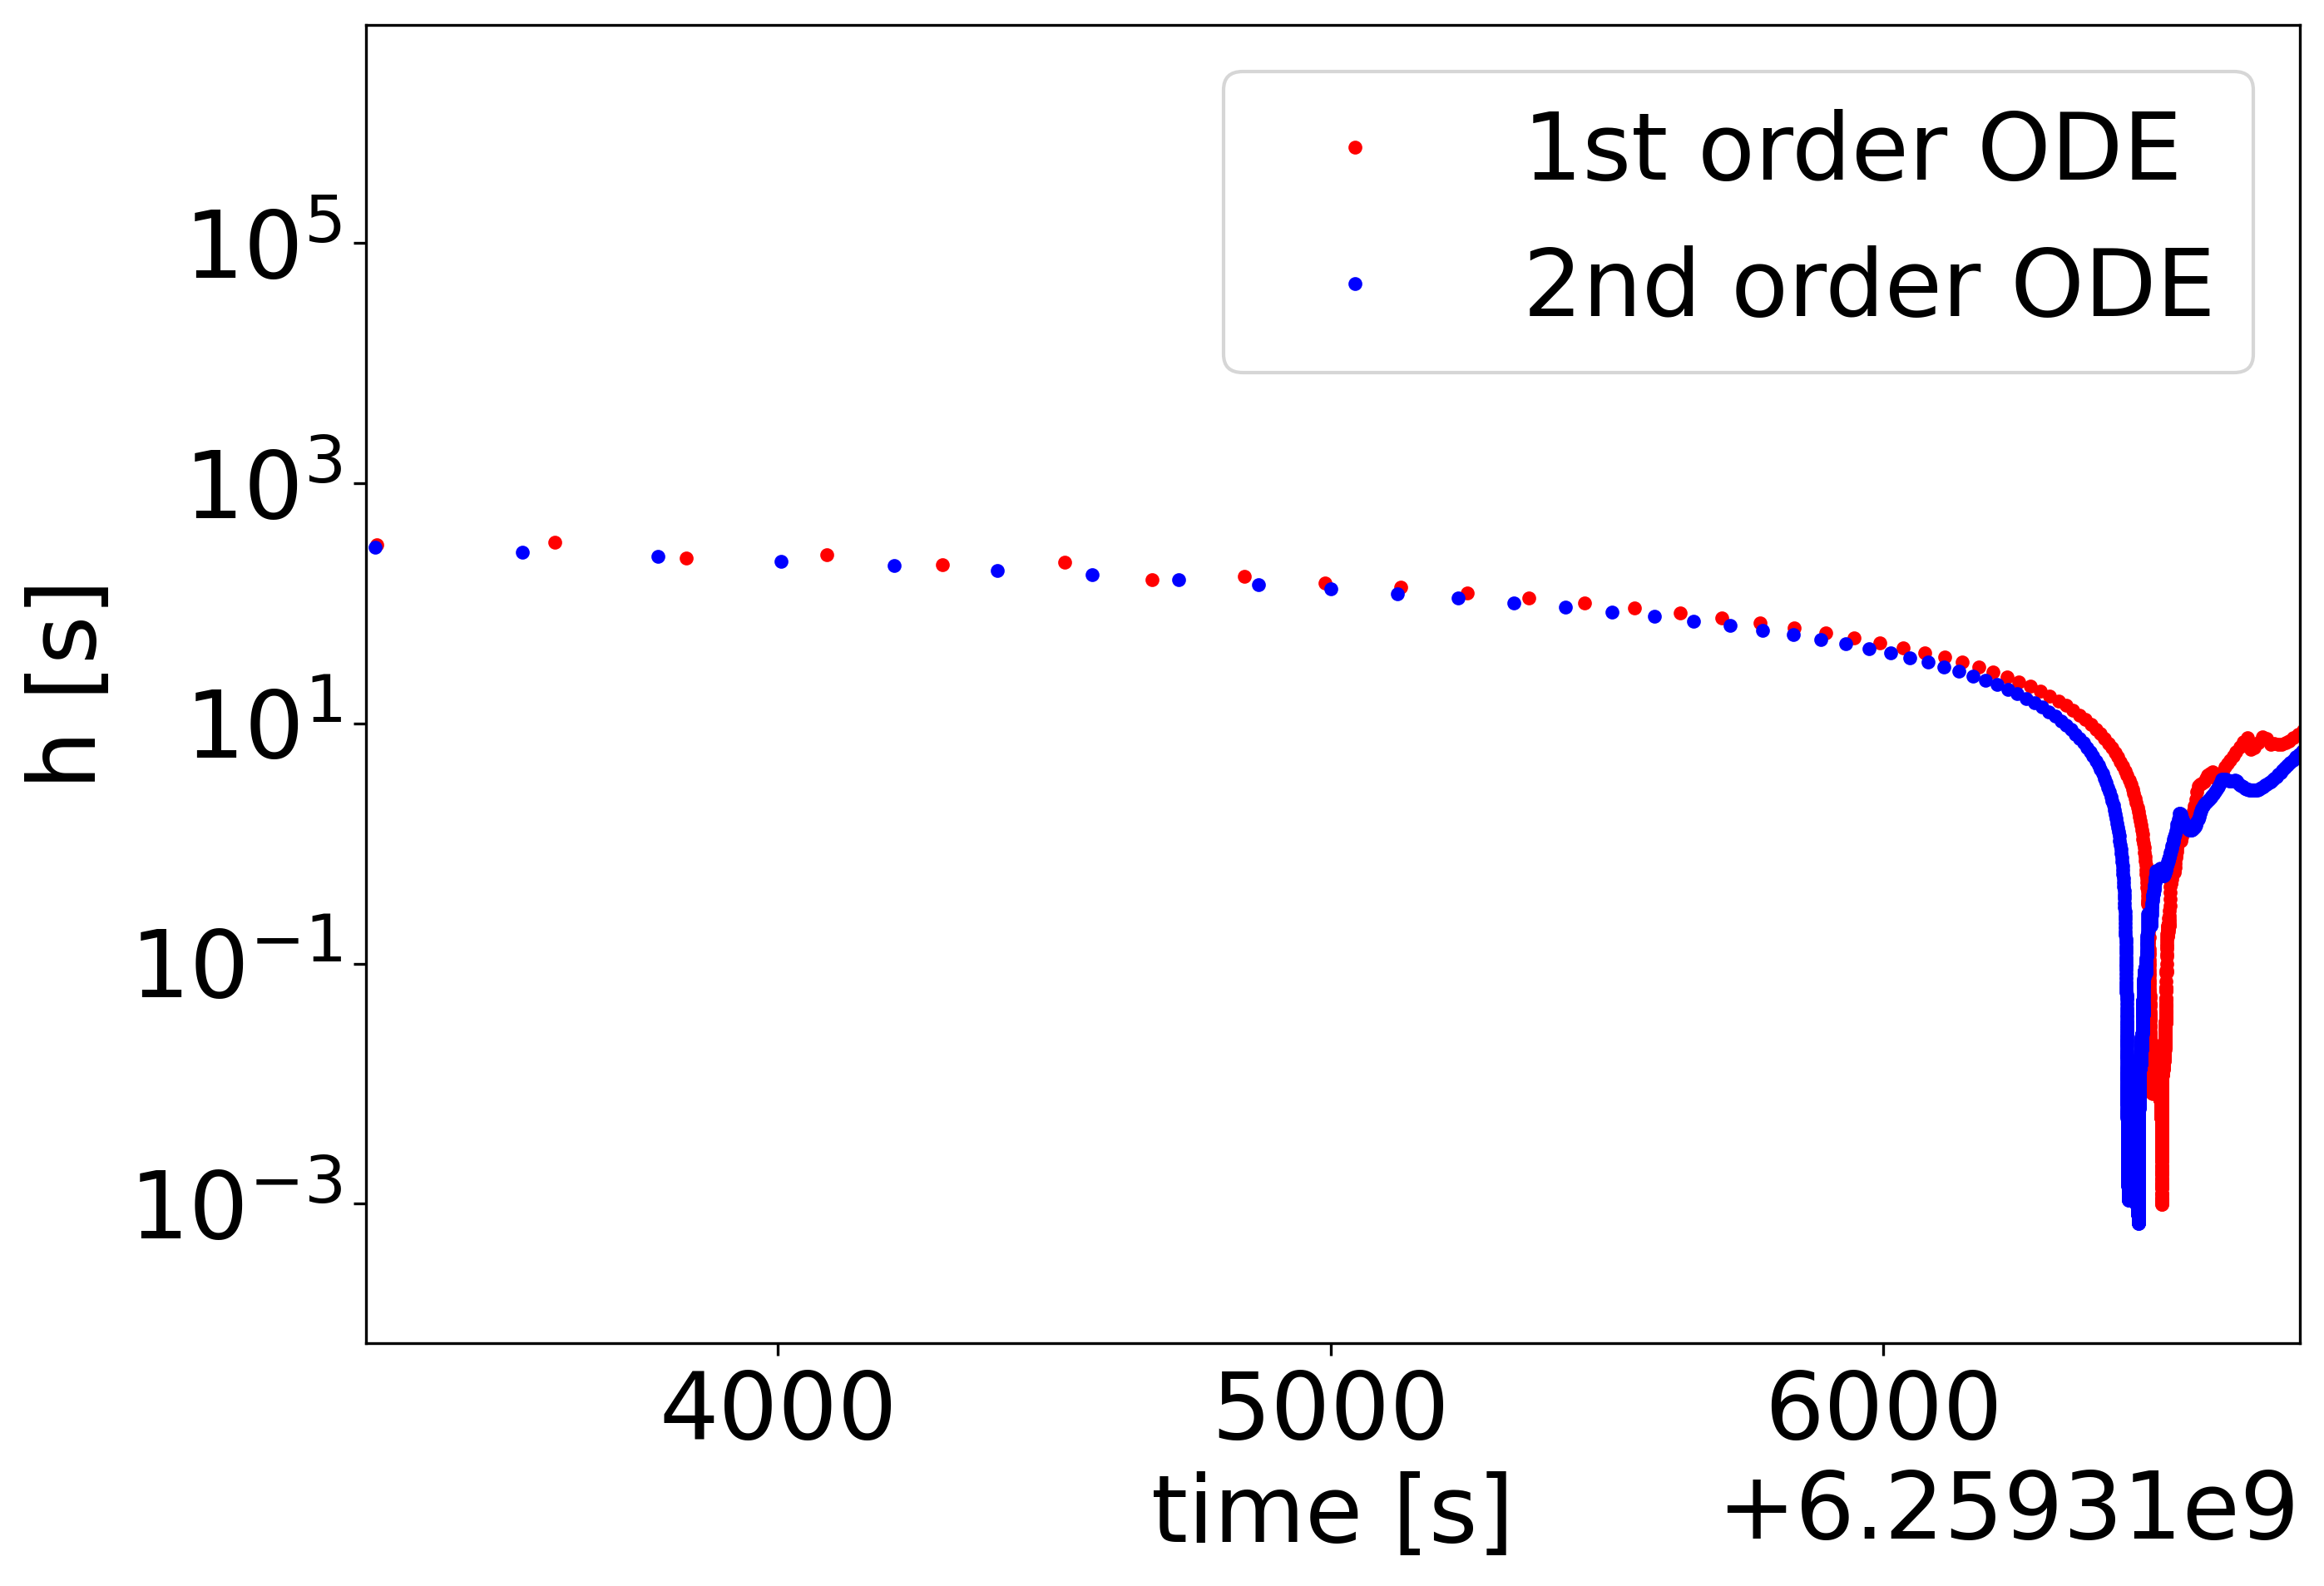
\includegraphics[width=1\textwidth]{images/TANDEMcompareFormulationstimeEvolutionDTearthquake.png}
       	\subcaption{Evolution of the earthquake event} 
    \end{subfigure}
    \caption{Evolution of the time step size $h$ for different solvers on the symmetric two-dimensional BP1 problem with 200 elements on the fault}
    \label{fig:timeEvolutionTANDEM_DT}
\end{figure}


\begin{figure}[H]
    \centering
    \begin{subfigure}{0.32\textwidth}
    	\centering
    	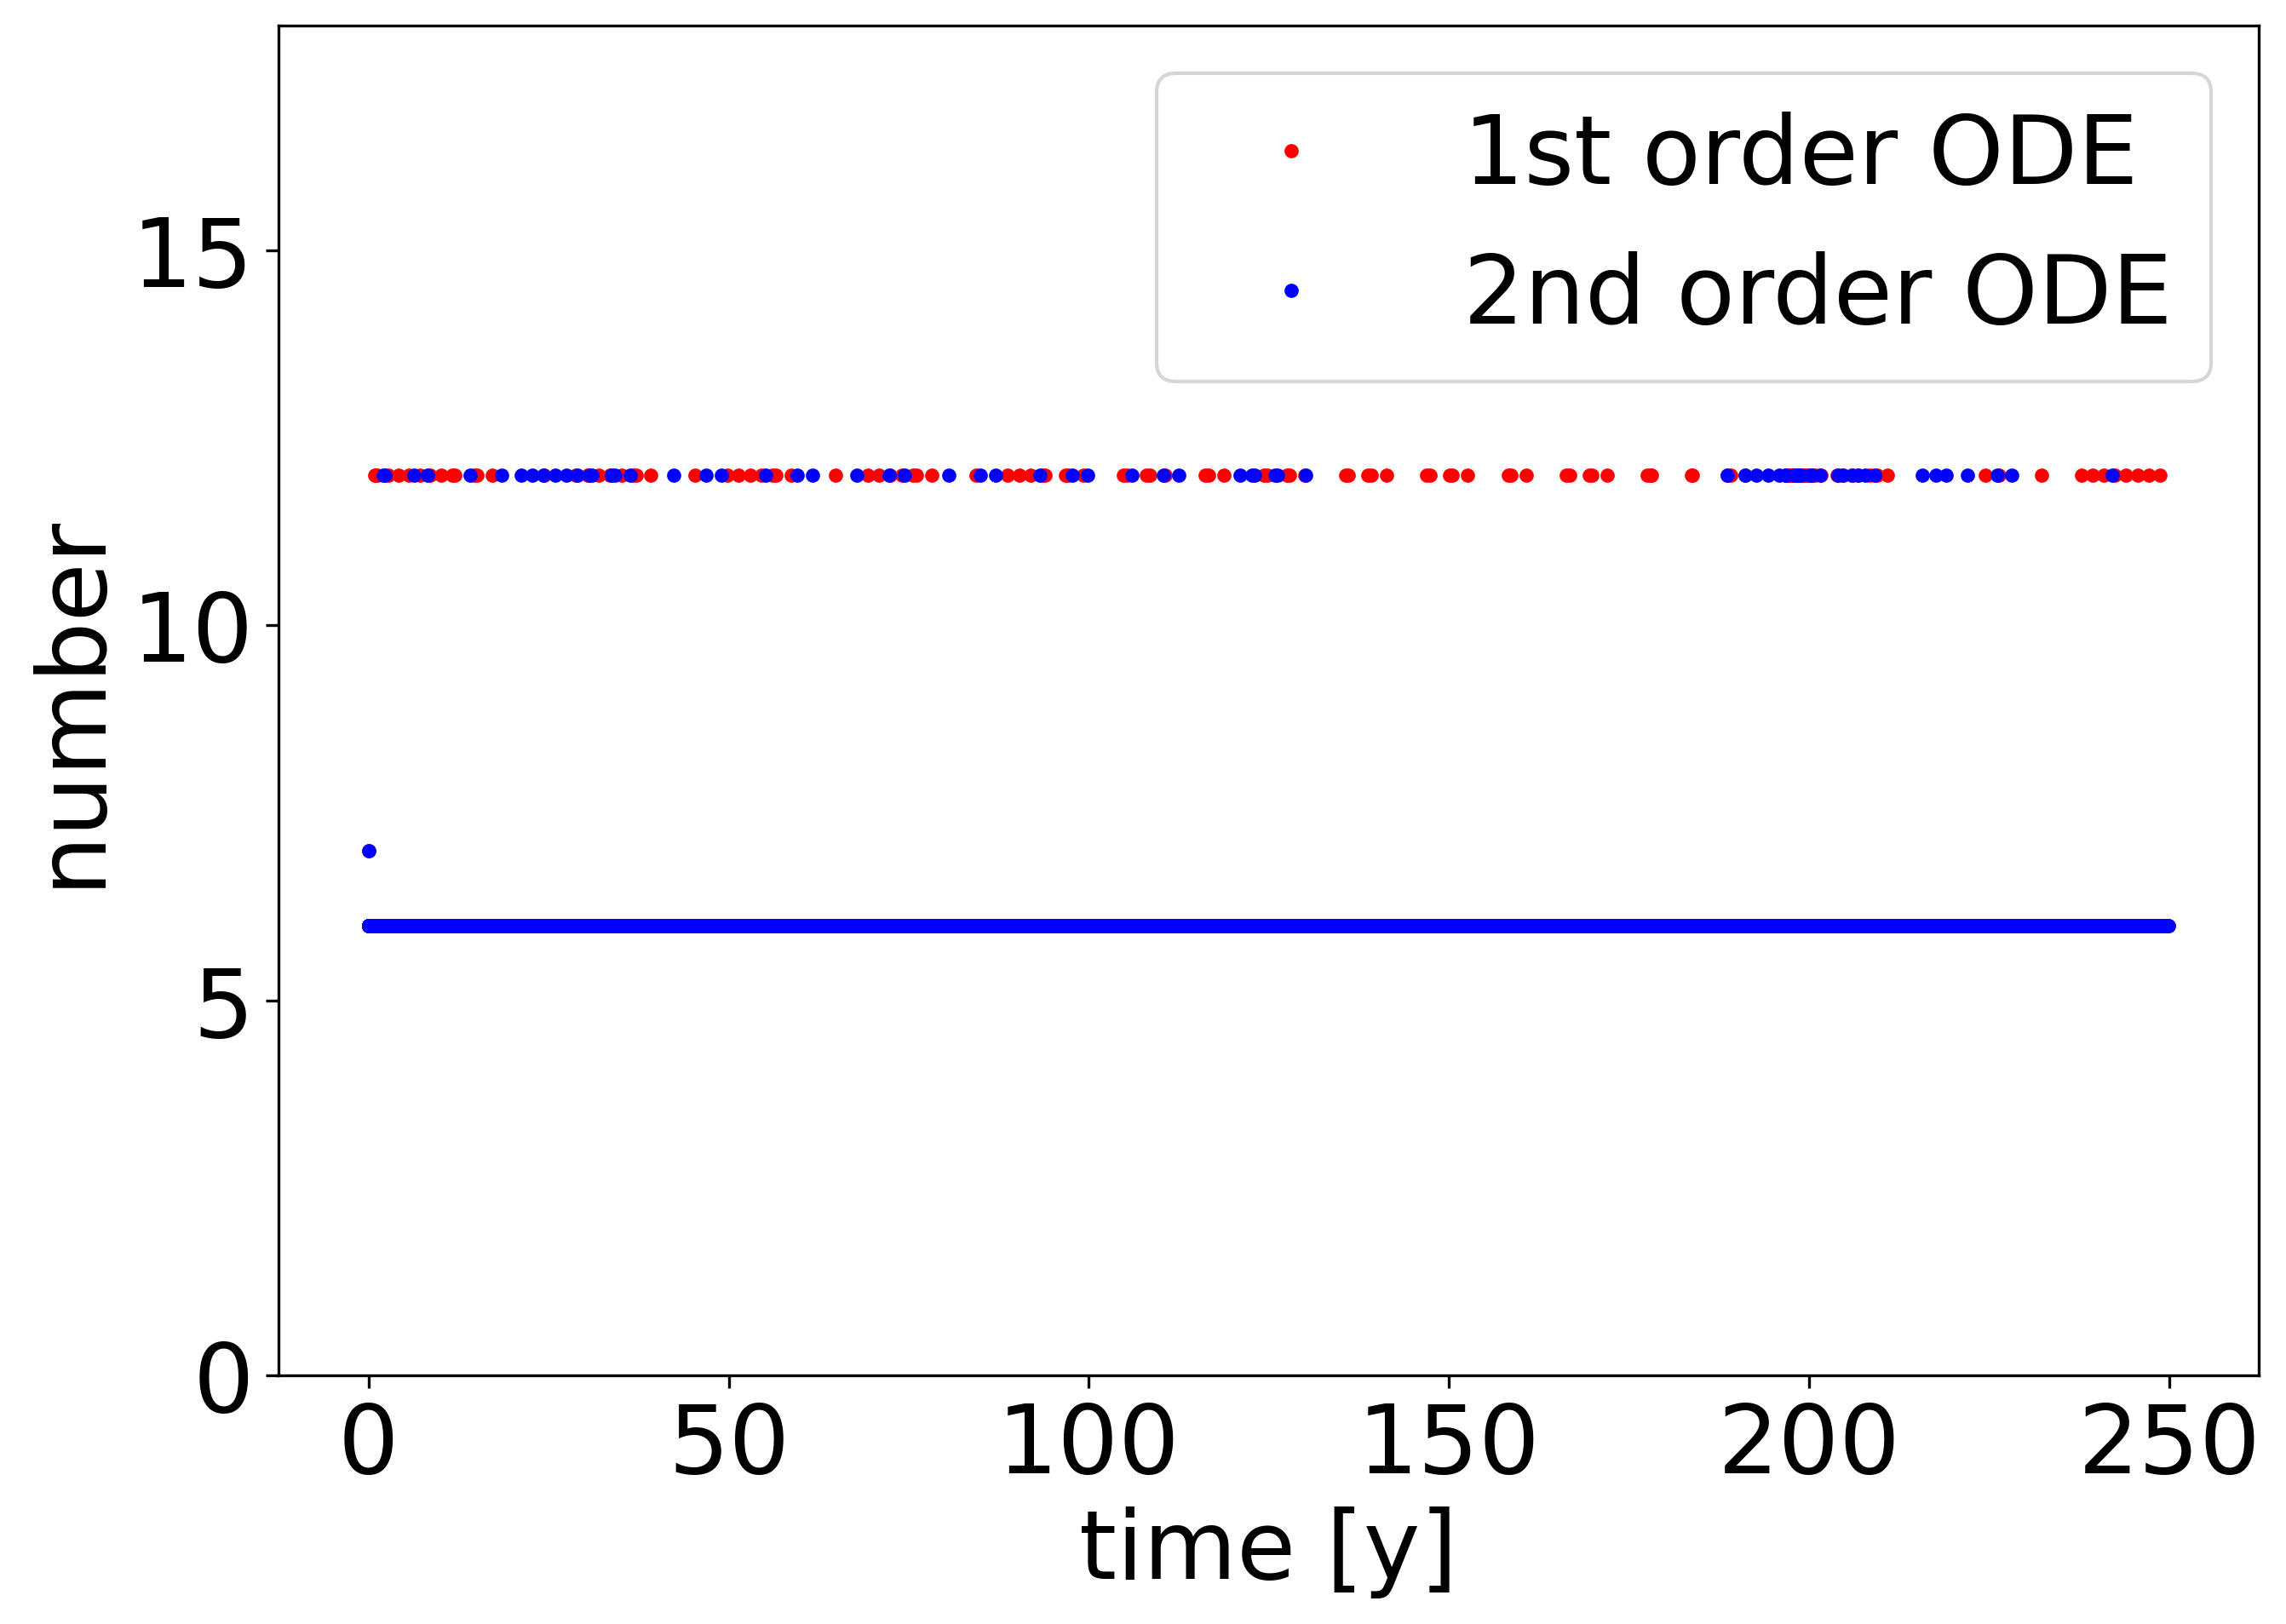
\includegraphics[width=1\textwidth]{images/TANDEMcompareFormulationstimeEvolutionRHSall.png}
       	\subcaption{Full simulation time} 
    \end{subfigure}
    \begin{subfigure}{0.32\textwidth}
    	\centering
    	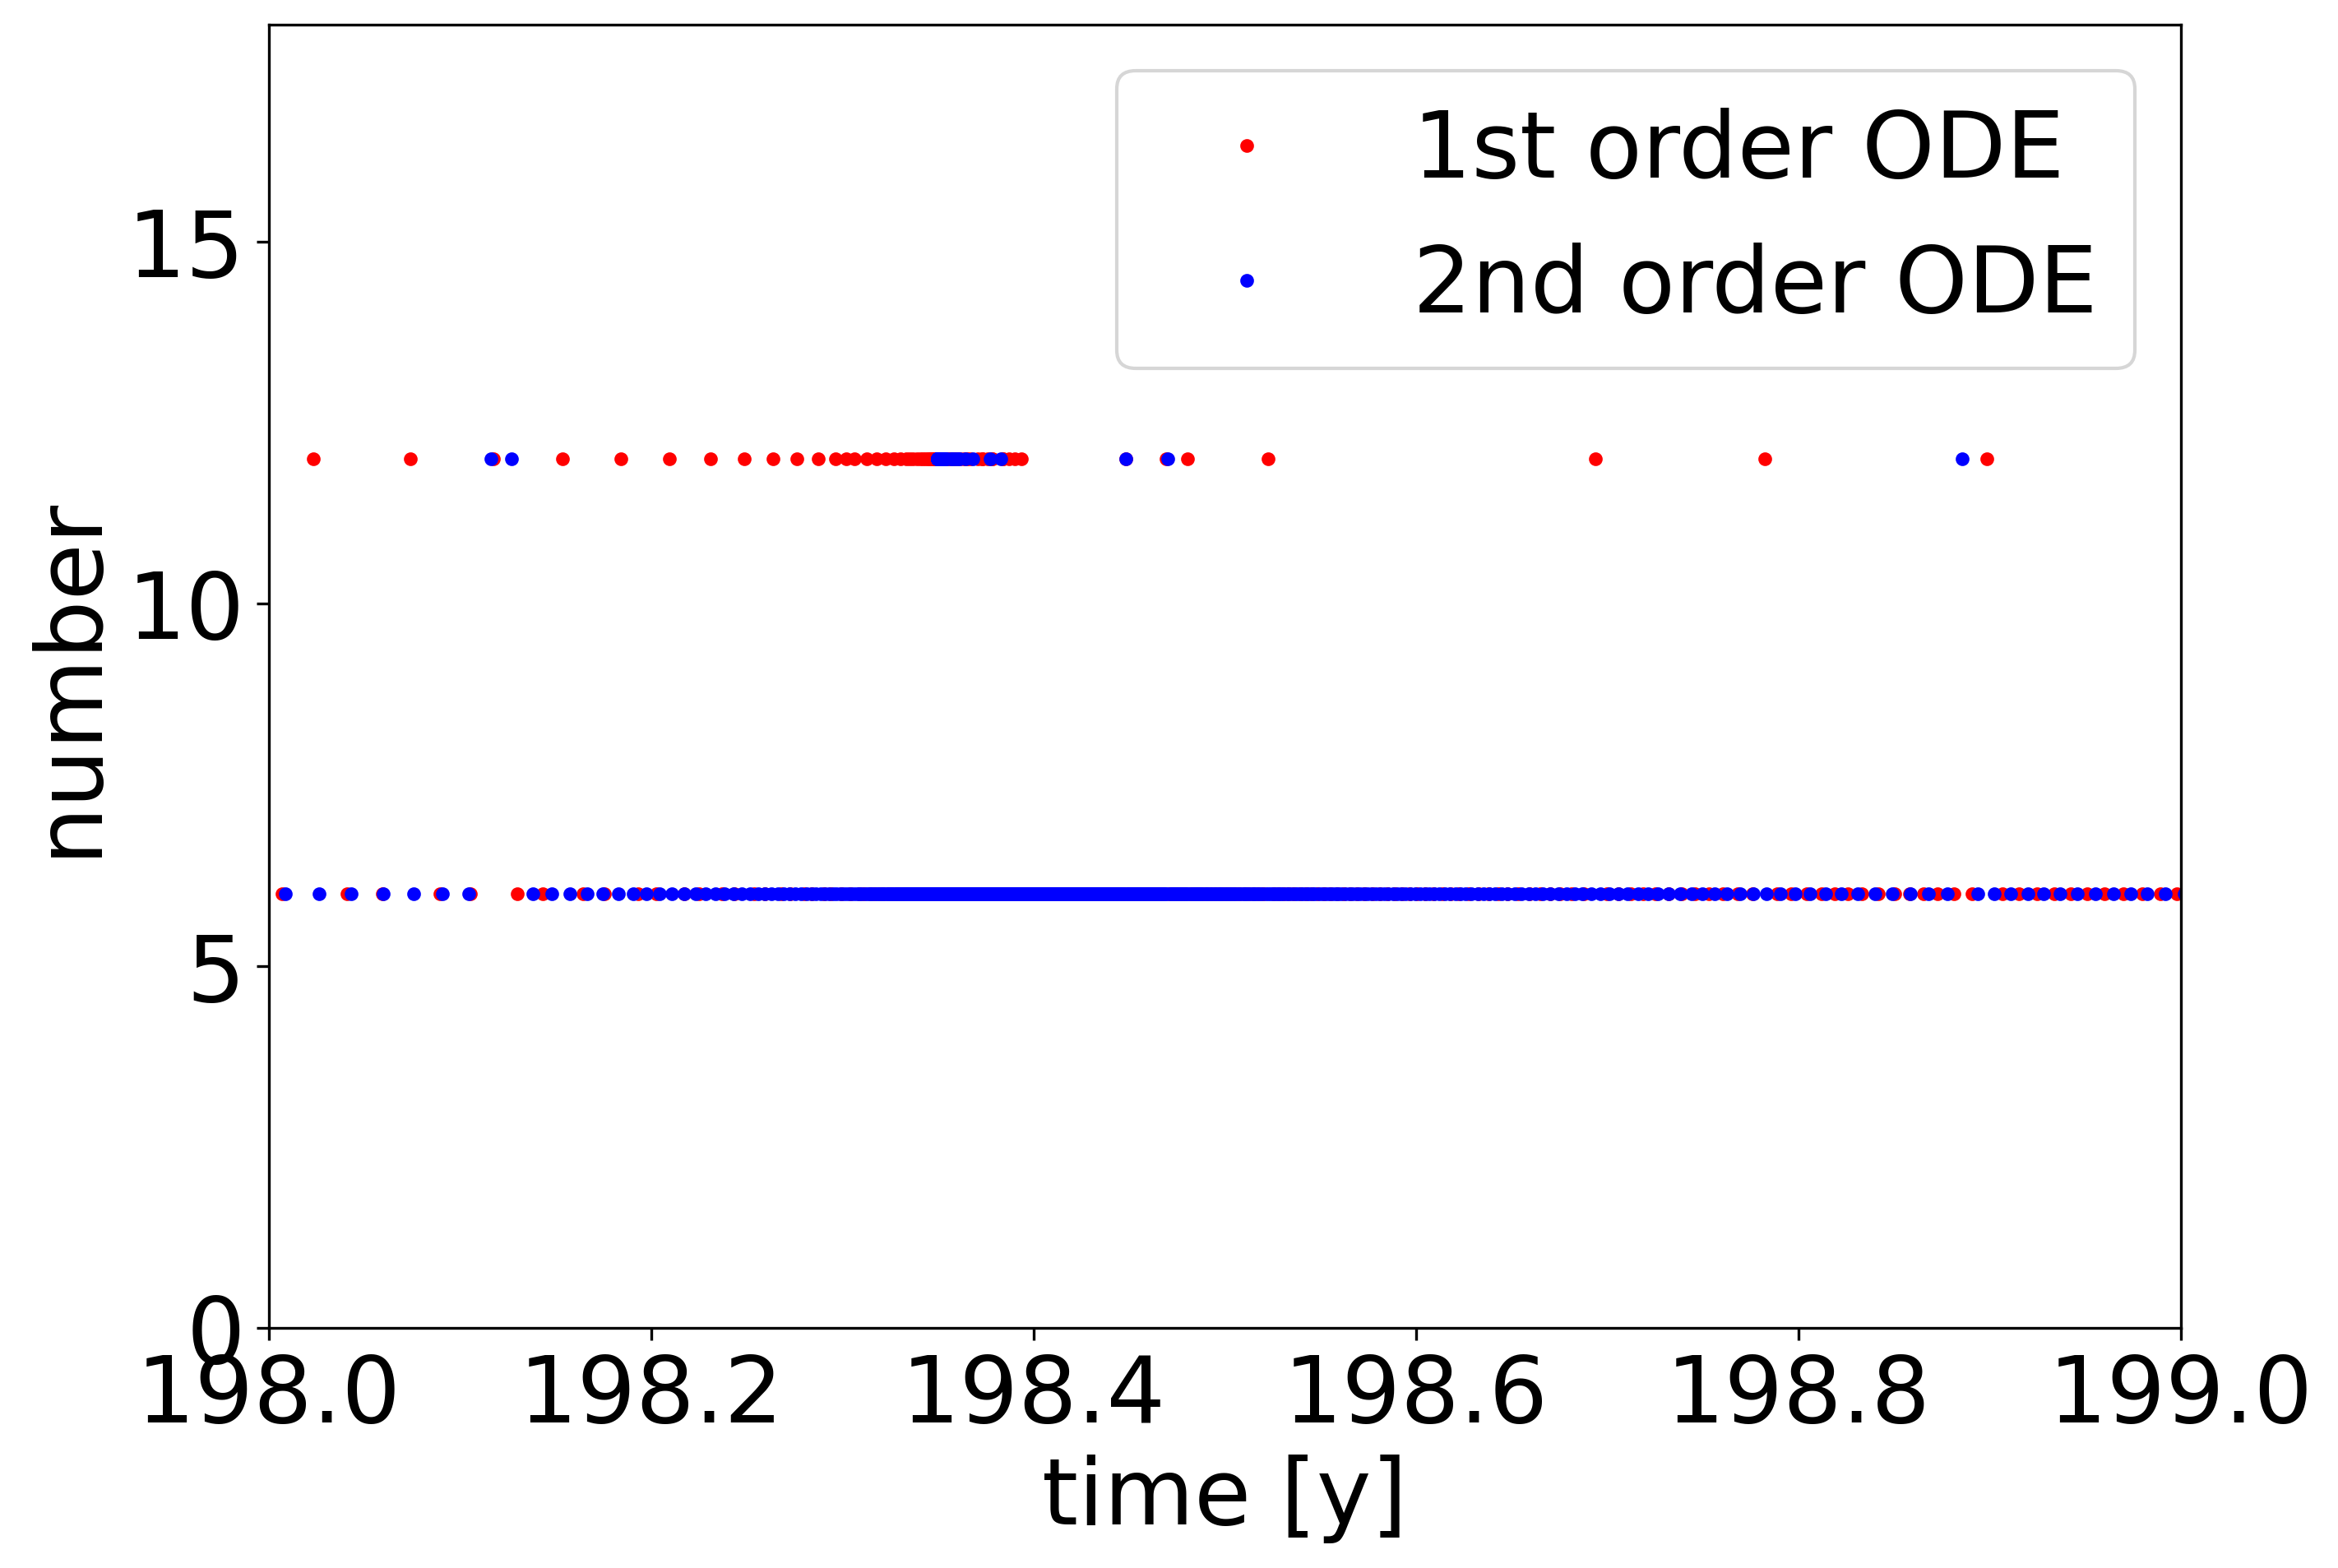
\includegraphics[width=1\textwidth]{images/TANDEMcompareFormulationstimeEvolutionRHSsurroundings.png}
       	\subcaption{Year of the earthquake} 
    \end{subfigure}
    \begin{subfigure}{0.32\textwidth}
    	\centering
    	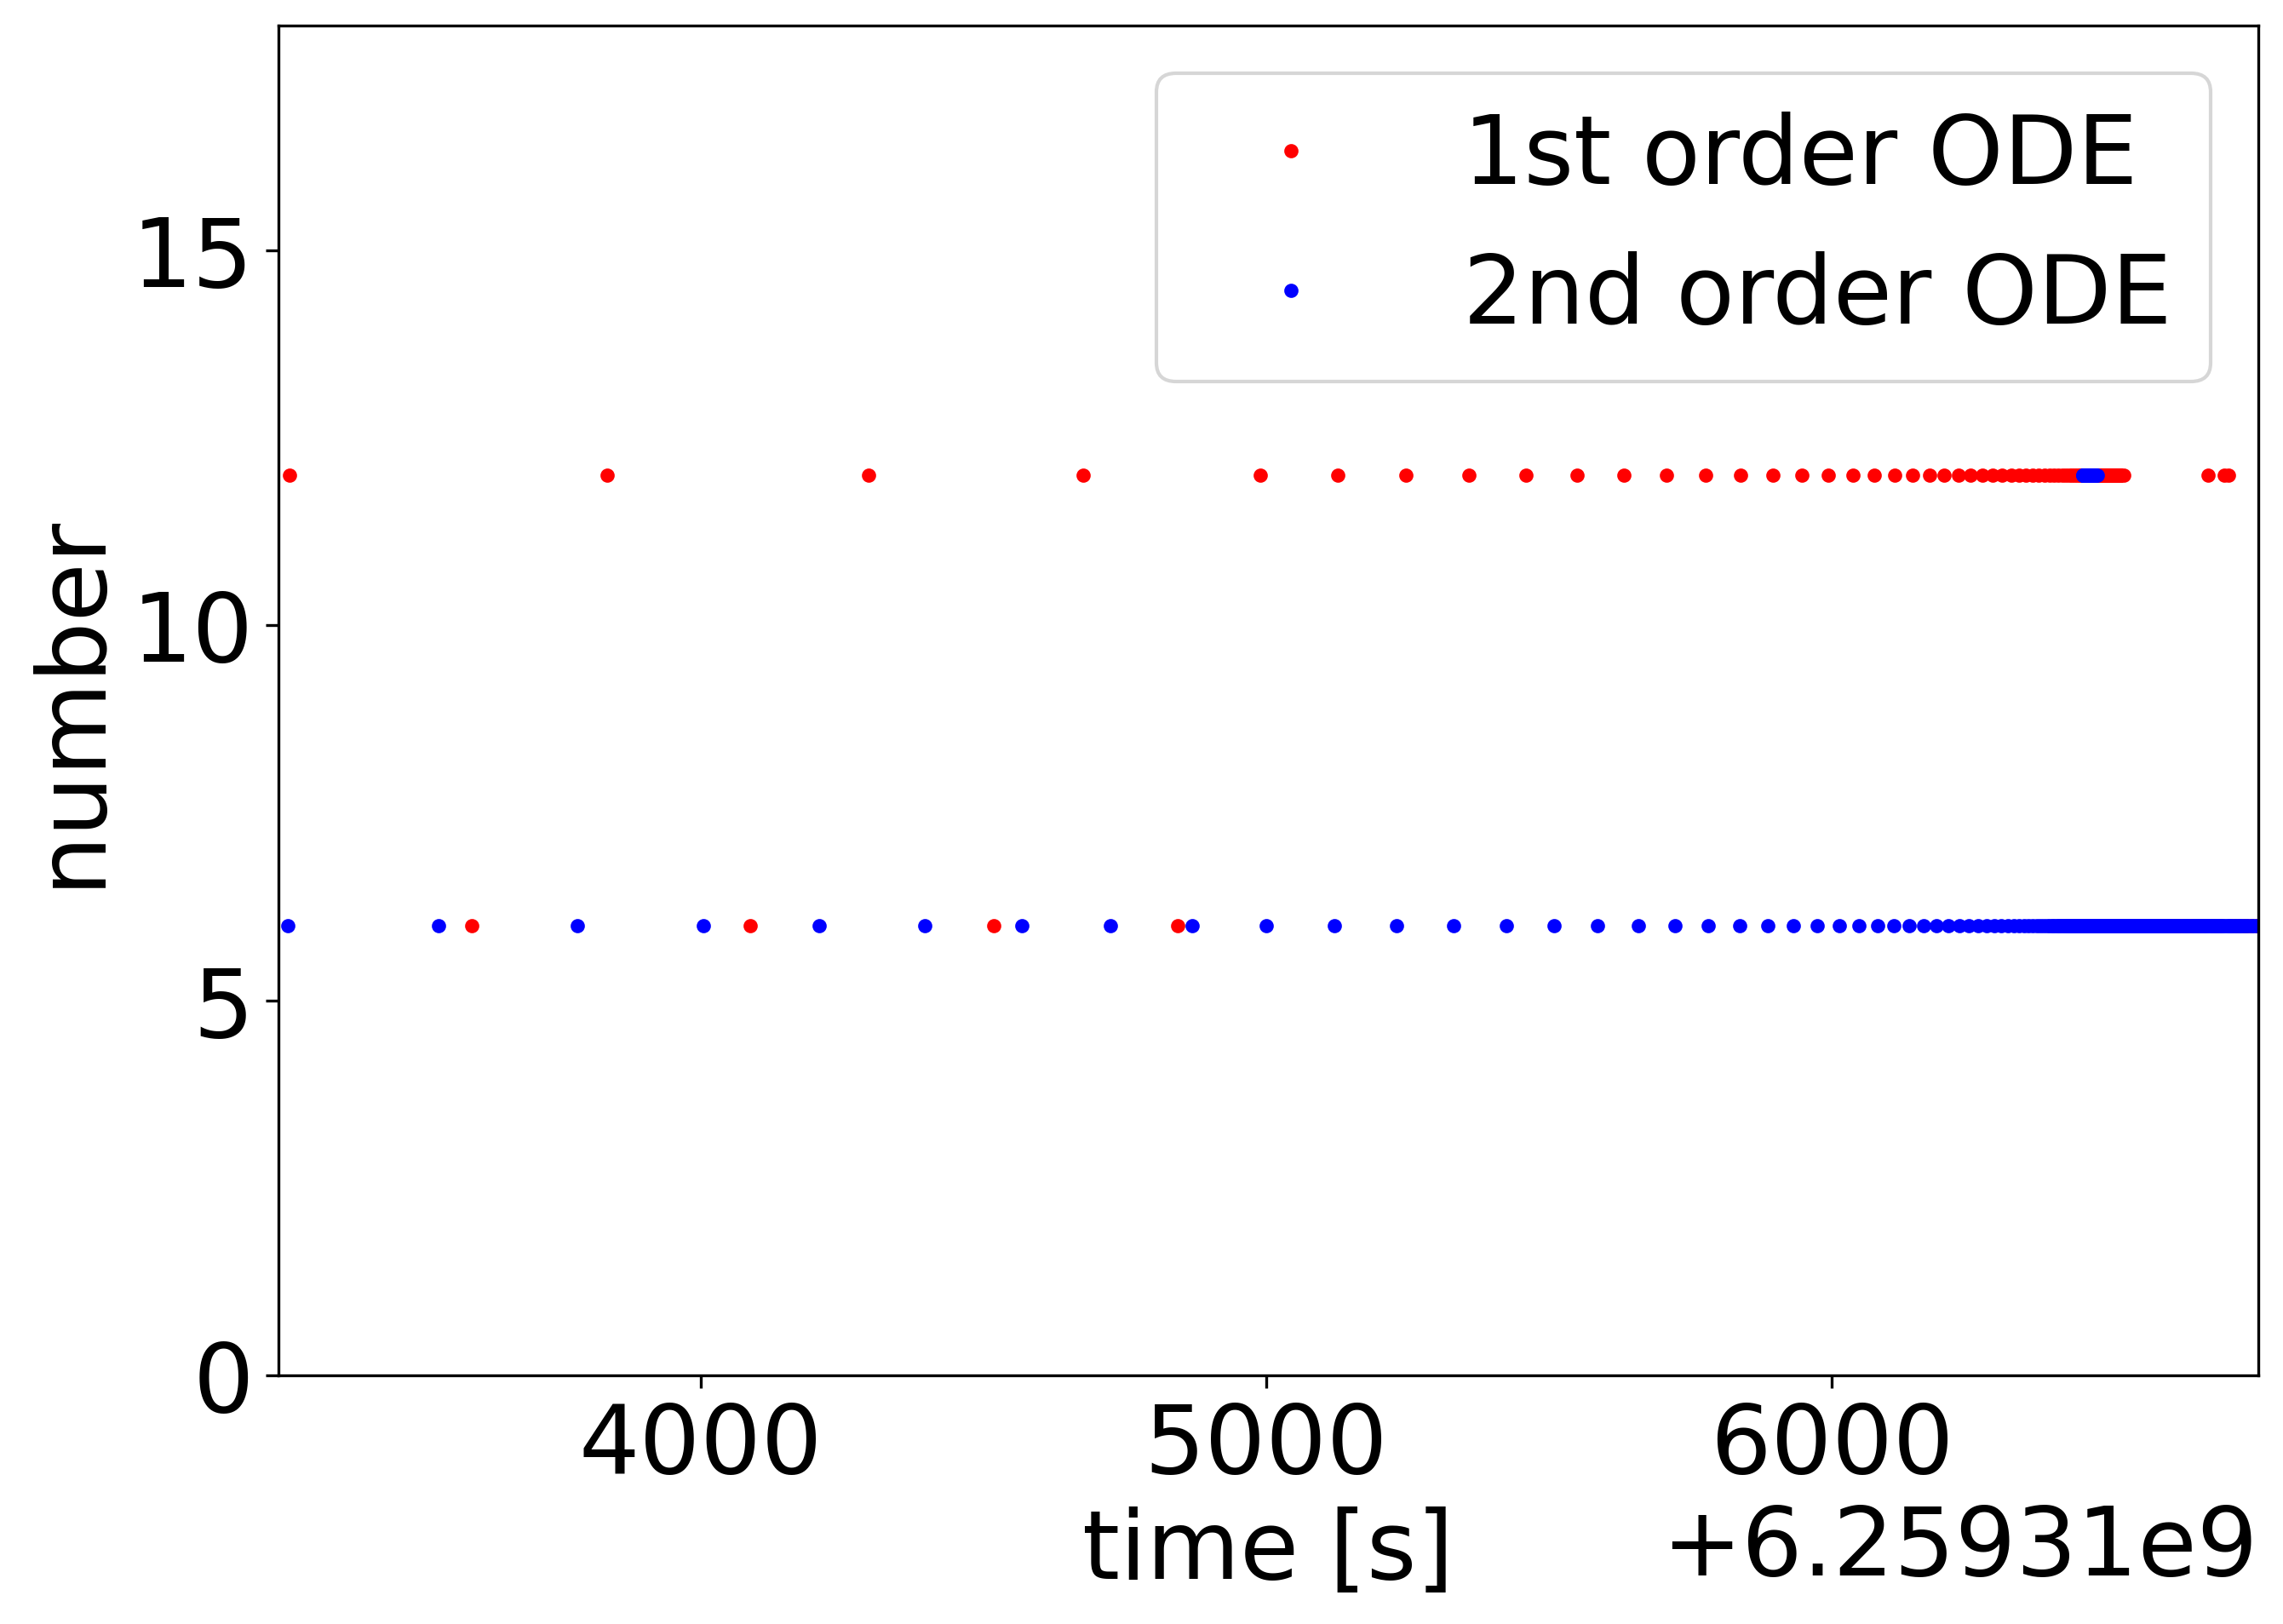
\includegraphics[width=1\textwidth]{images/TANDEMcompareFormulationstimeEvolutionRHSearthquake.png}
       	\subcaption{Evolution of the earthquake event} 
    \end{subfigure}
    \caption{Number of evaluations of the right hand side of the ODE in each time iteration for different solvers on the symmetric two-dimensional BP1 problem with 200 elements on the fault \newline
    \textbf{Legend:} \textcolor{red}{---} 1st order ODE formulation, \textcolor{blue}{---} 2nd order ODE formulation, \textcolor{green}{---} extended DAE formulation, \textcolor{yellow}{---} compact DAE formulation }
    \label{fig:timeEvolutionTANDEM_RHS}
\end{figure}

\subsection{Error estimation of the 2nd order ODE formulation}
Despite the lack of an analytic solution to the problem, this formulation of the problem offers a very powerful tool to evaluate the accuracy of the results. Since the slip rate is not calculated from the friction law anymore, it is not ensured that it is always equal to 0 up to numerical precision, as it was the case in the first order formulations of the SEAS problem. We could then evaluate the friction law at every timestep to assess the accuracy of the numerical integration. A large deviation from 0 of the absolute value of the friction law at a given timestep means that the integrator provides poor results. For a standard execution of the simulation with the second order formulation, this metric is not available, since the evaluation of $\tau$ in the friction law requires to solve the Poisson problem, and the big advantage of the new formulation is exactly not to solve this system. For the following graphs, The value of the friction law has been exceptionally calculated. \\

For the first set of pictures, a very small domain with 5 fault elements has been chosen to be able to observe the evolution of the quantities over a long period of time. The tolerances for the slip and the state variable have been fixed to $10^{-7}$. \autoref{fig:timeEvolution_2ndOrderODE_differentTolerances} shows the maximum value of the friction law for varying relative relative tolerances for $V$, and the absolute tolerance is fixed to 0. From the initial condition, the slip rate is calculated to fulfill the friction law up to numerical precision, at about $10^{-15}$. After some time steps, this high precision is lost, and at every earthquake event, the difference increases sharply. Overall, the logarithmic shape of the curves indicate a linear decrease of accuracy with time, It seems that, at every evaluation of the right-hand side function, for one given tolerance of $V$, a certain local truncation error is added to the residual of the friction law. At an earthquake, much more timesteps are required and the sum of the local truncation errors sum up to form an apparent sharp increase in the global error. For lower tolerances in $V$, the increase of the error at every evaluation is smaller the accuracy is higher. This hypothesis is confirmed by \autoref{fig:timeEvolution_LTE_2ndOrderODE_differentTolerances}, which shows the absolute change of the friction law per timestep. It can be considered somehow as an estimate for the local truncation error (LTE), as it describes how the error increases at each step. For a given tolerance in the slip rate, an upper bound for the LTE can be observed. During the earthquake, the LTE is actually much lower than in the aseismic slip. Only the high number of steps required for this event result in the apparent sharp increase of the total error. 

\begin{figure}[H]
	\centering
	\begin{subfigure}{0.45\textwidth}
		\centering
		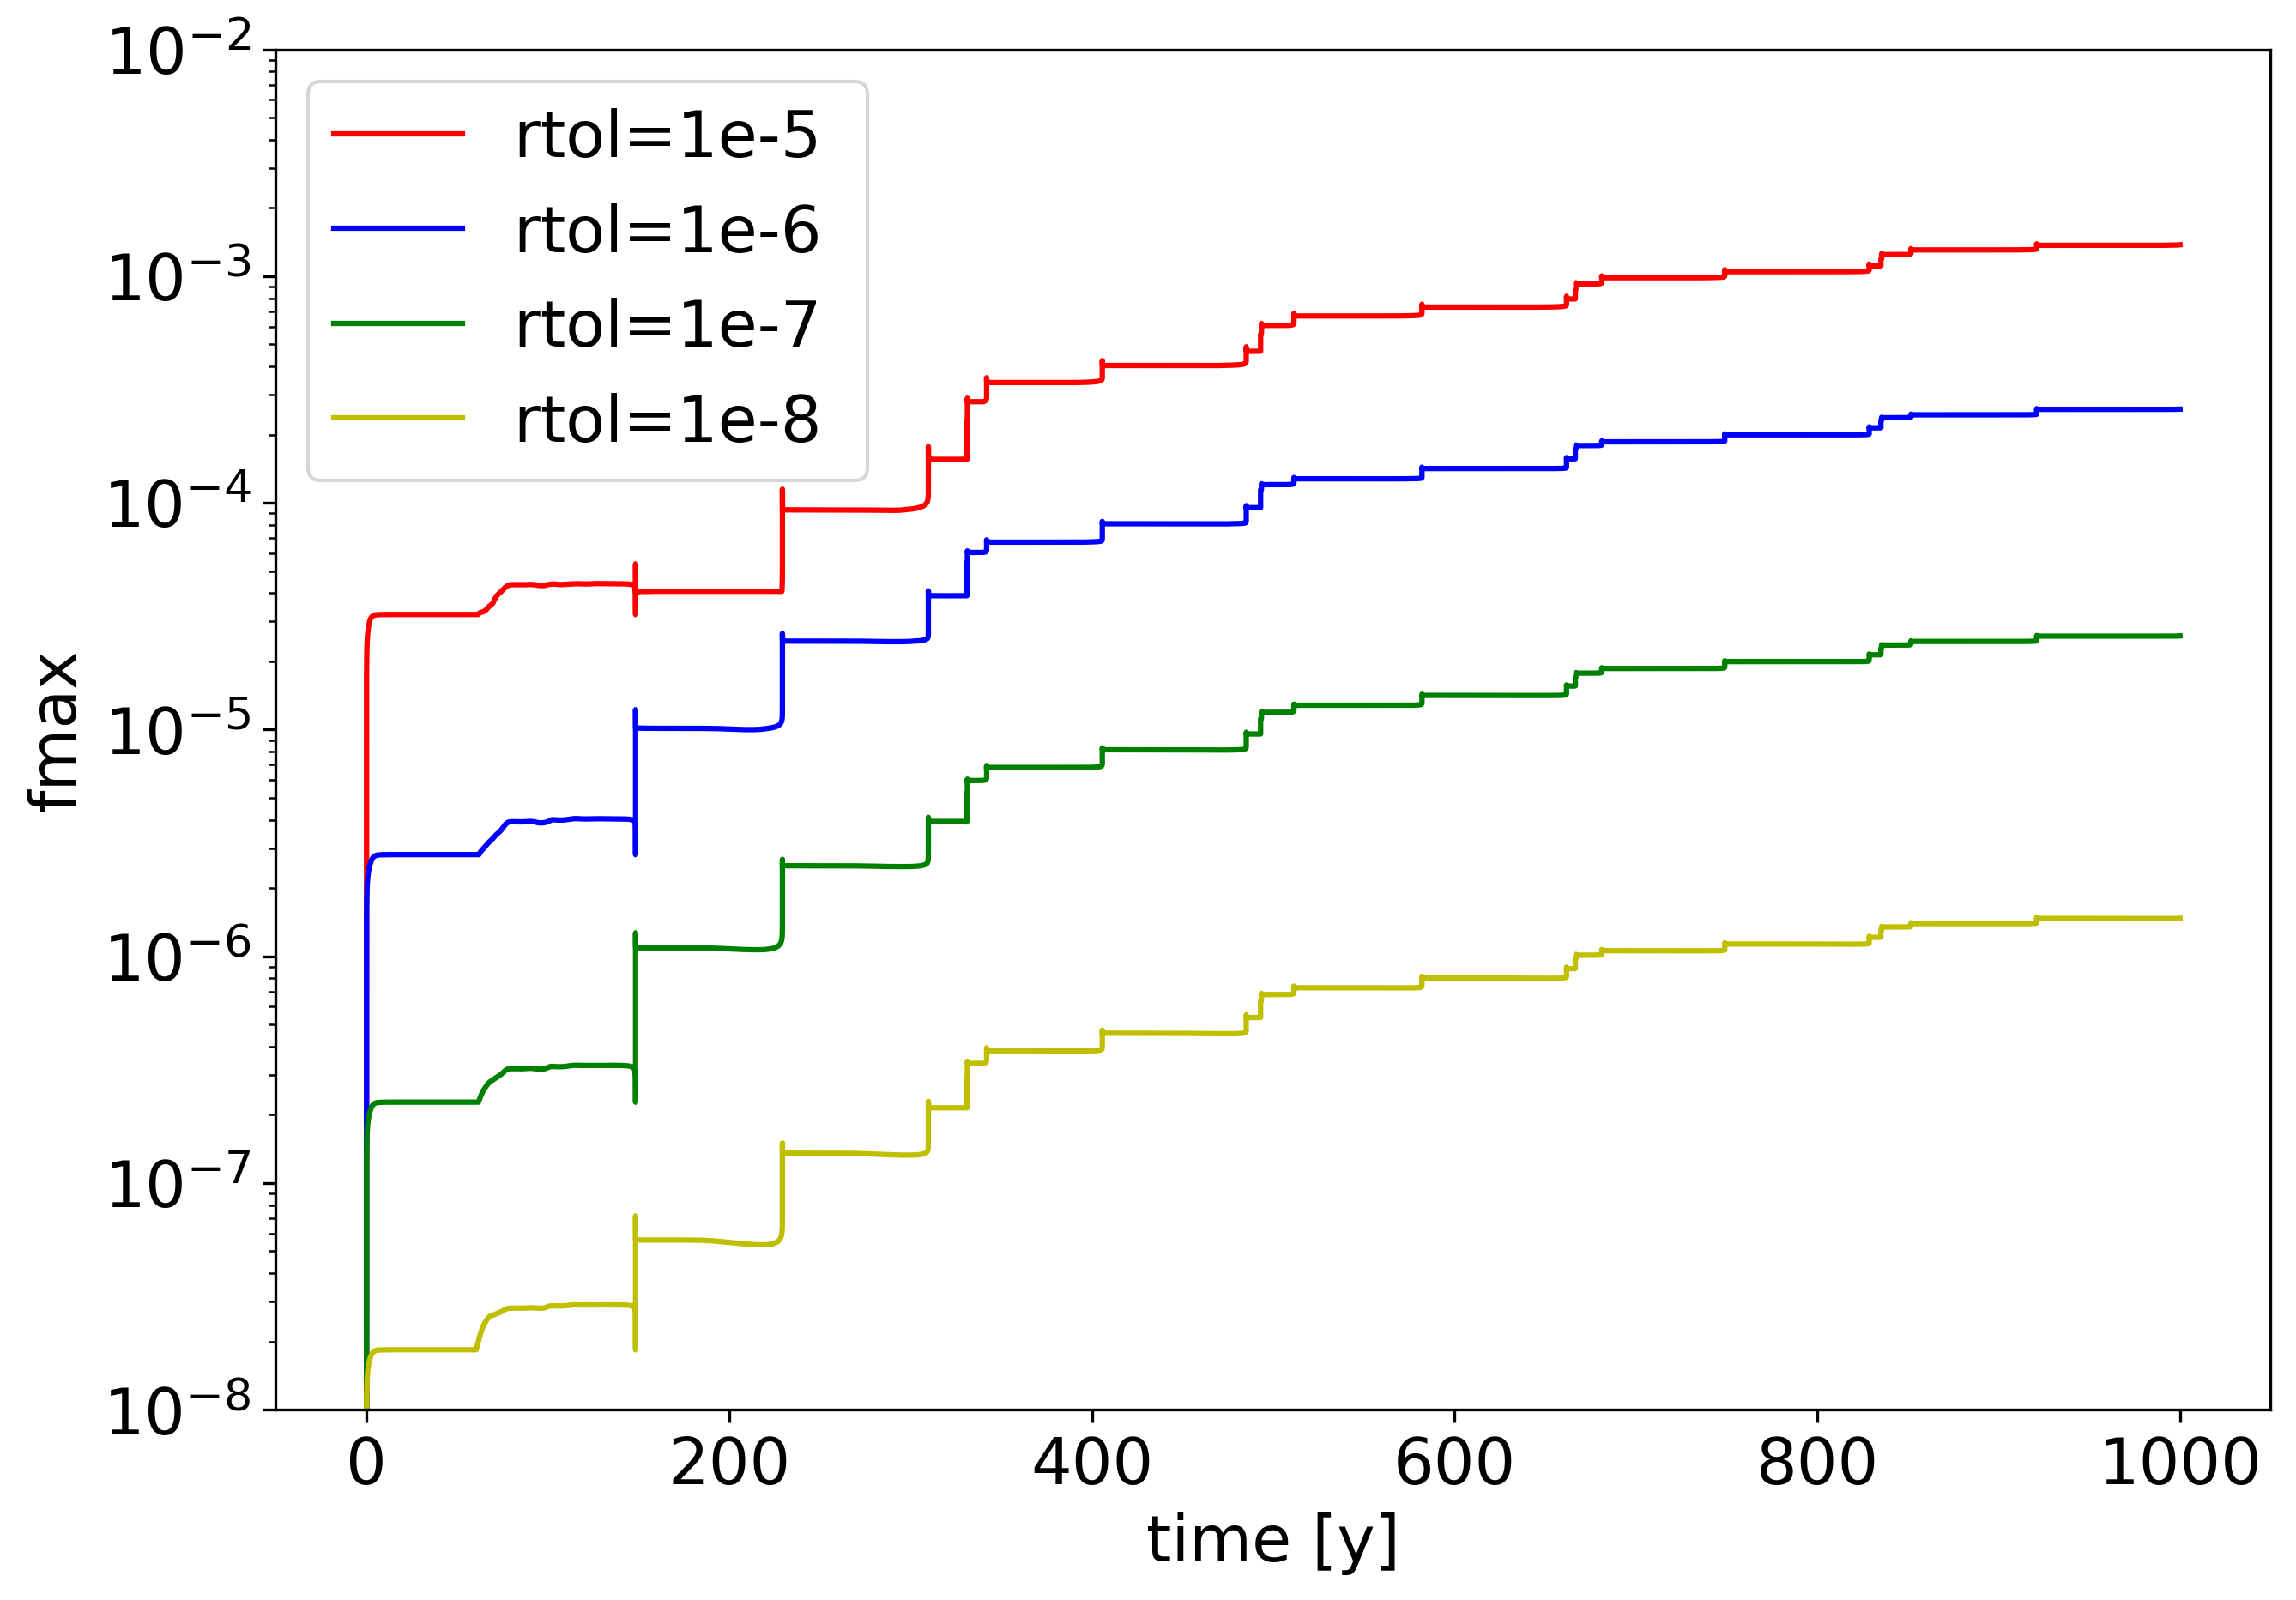
\includegraphics[width=1\textwidth]{images/TANDEMtimeEvolutionFExtendedODEDifferentTolerances.png}
		\subcaption{Maximum absolute value of the friction law} 
		\label{fig:timeEvolution_2ndOrderODE_differentTolerances}
	\end{subfigure}
	\begin{subfigure}{0.45\textwidth}
		\centering
		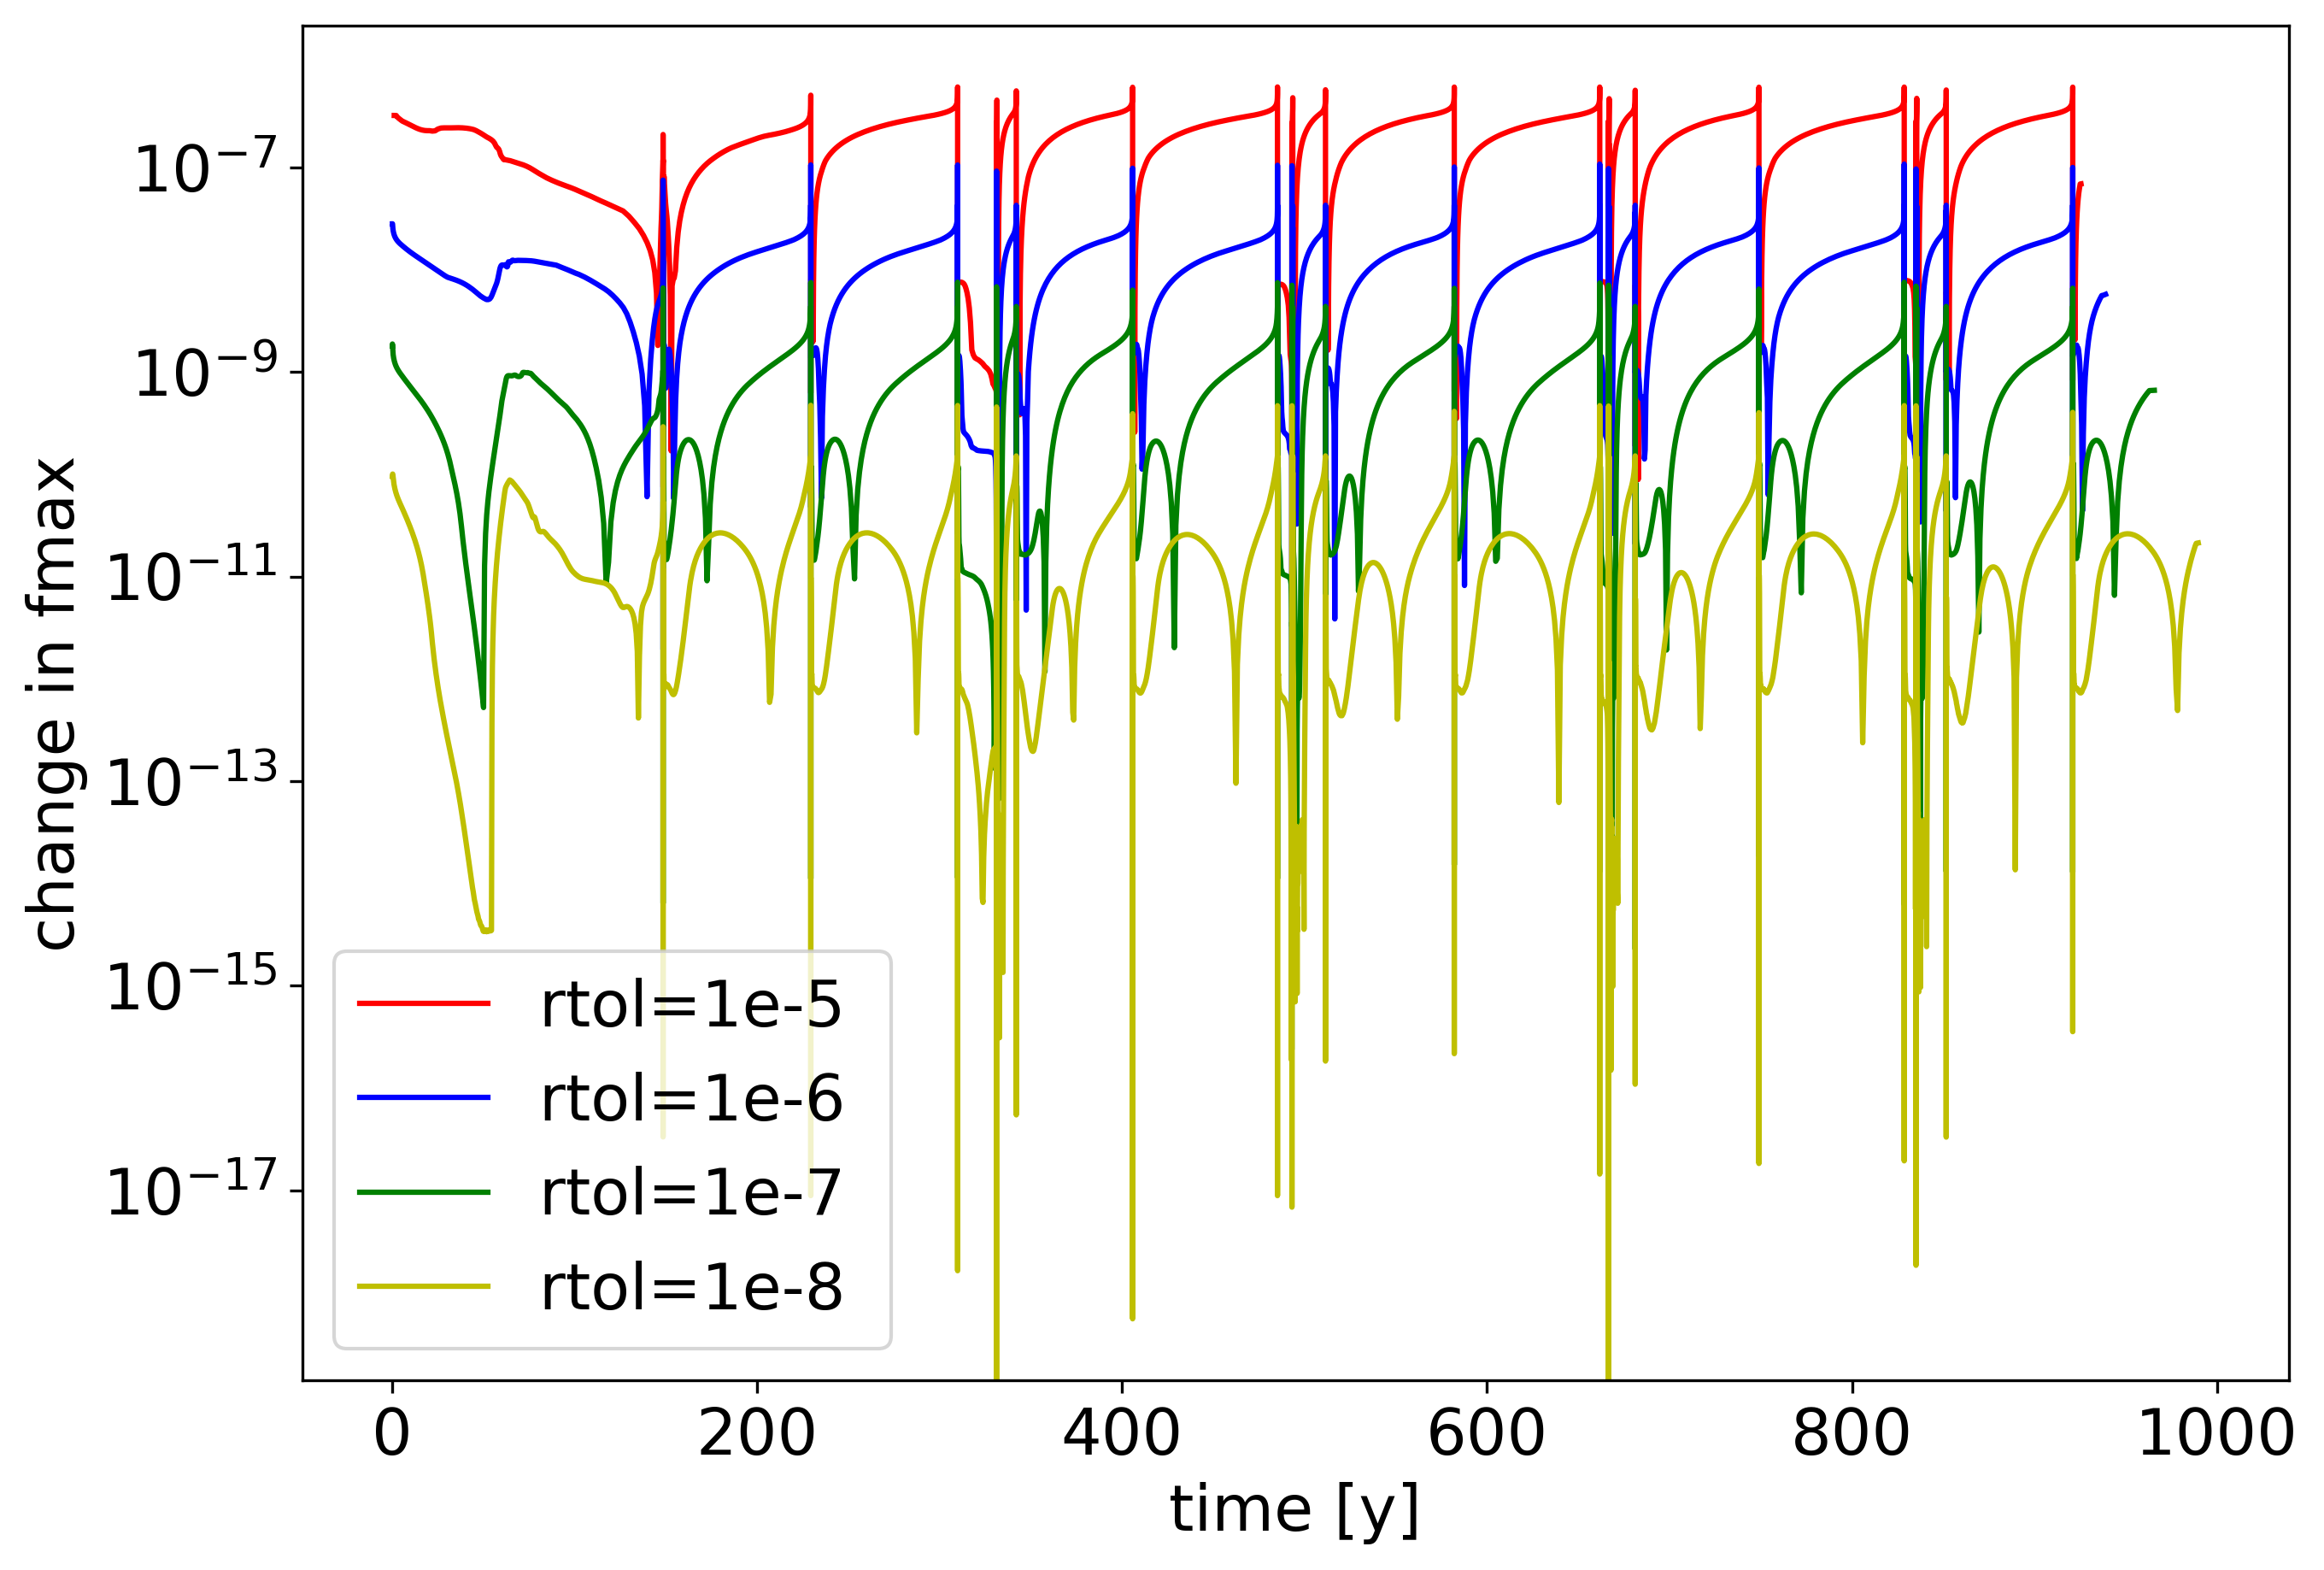
\includegraphics[width=1\textwidth]{images/TANDEMtimeEvolutionFLTEExtendedODEDifferentTolerances.png}
		\subcaption{Absolute change of the friciton law per timestep, averaged over 50 timesteps} 
		\label{fig:timeEvolution_LTE_2ndOrderODE_differentTolerances}
	\end{subfigure}
	\caption{Evolution of the value of the friction law of the 2nd order formulation with 5 elements on the fault over 1000 years with varying relative tolerances in the slip rate $V$}
\end{figure}

The local truncation error seems to depend linearly on the tolerance for the slip rate, and a similar dependency is to be expected with respect to the tolerances of the slip $S$ and $\psi$, since these quantities are also required to evaluate the friction law. Next, we investigate whether other parameters, such as the spatial discretization, have an effect on the global error too. For a fixed relative tolerance for the slip of $10^{-7}$, the simulation has been executed for different spatial resolutions and the evolution of the friction law in each case is shown in \autoref{fig:timeEvolution_2ndOrderODE_differentSizes}. Since each fault elements contains three fault nodes, one has to multiply $n$ by three to obtain the total number of simulated fault nodes. At the beginning, all domain sizes have a similar accuracy, but after some earthquakes, it seems that the error in domains with higher resolution increases less fast. However, in \autoref{fig:timeEvolution_LTE_2ndOrderODE_differentSizes}, it is hard to distinguish separate upper bounds for the local truncation error with different domain sizes. The better performance of larger domains is rather due to the overall higher accuracy of simulations with higher resolutions and to a lower incidence of earthquakes, than due to a reduction of the LTE. 

\begin{figure}[H]
	\centering
	\begin{subfigure}{0.45\textwidth}
		\centering
		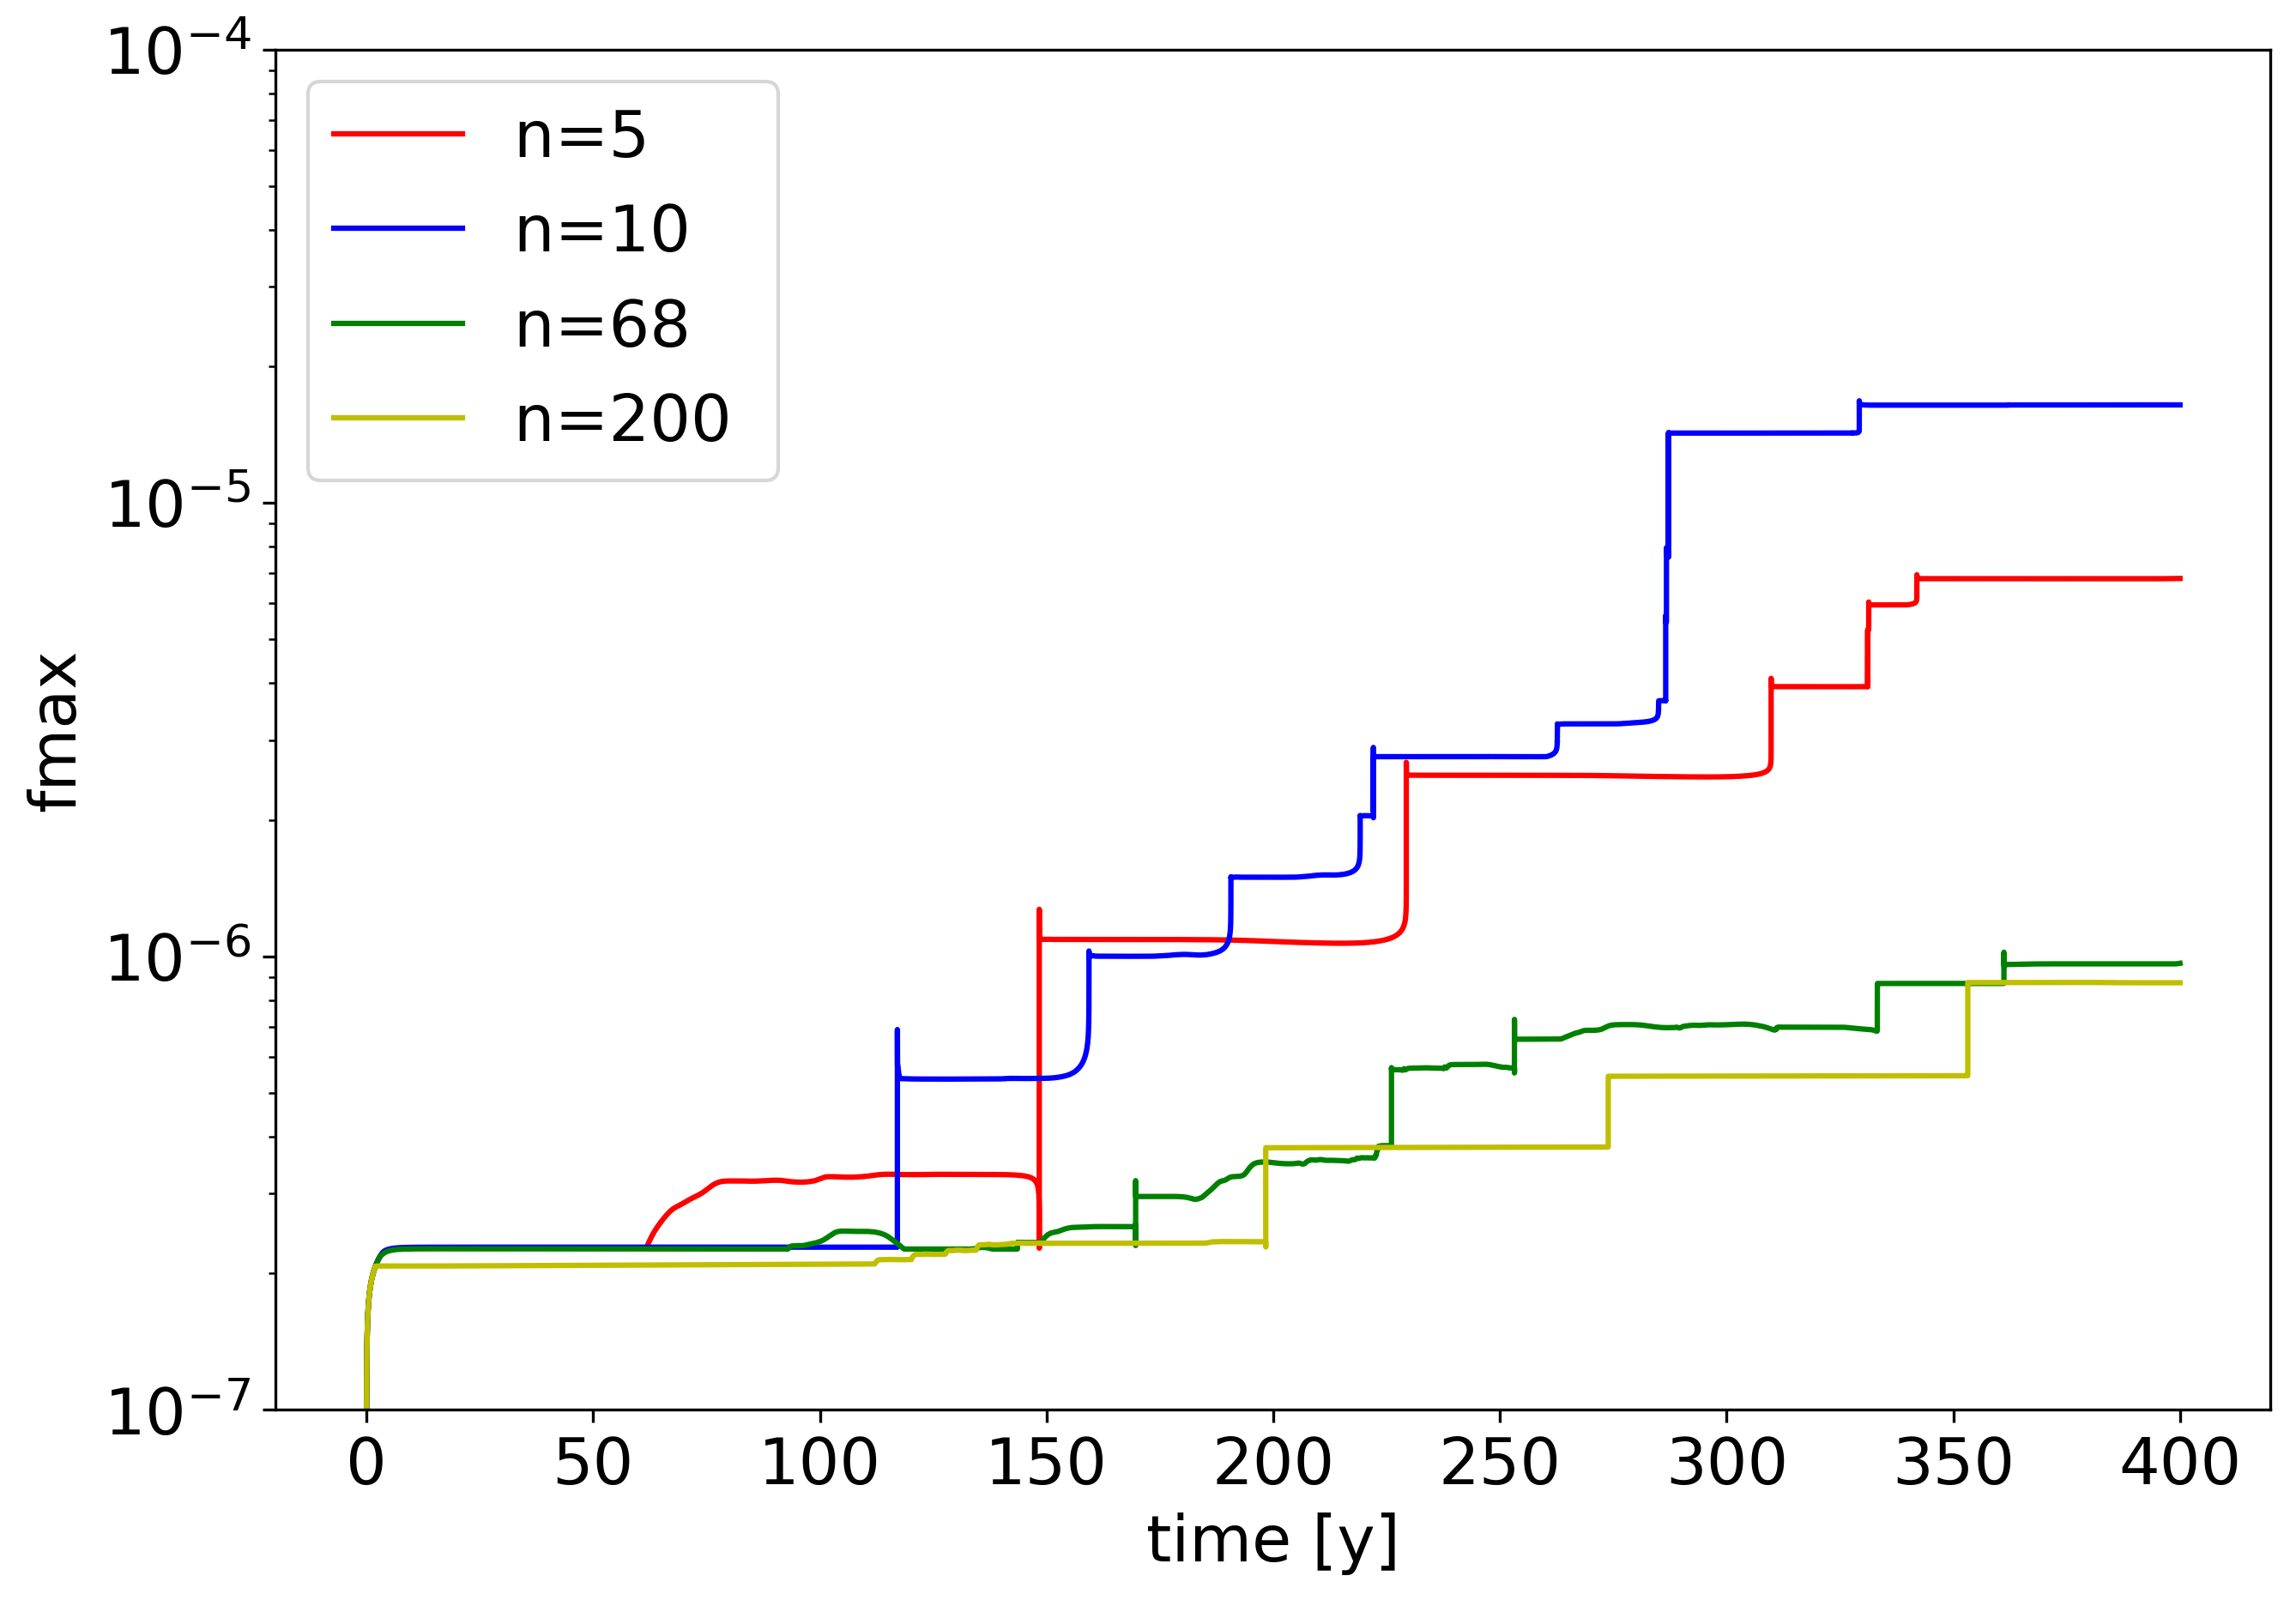
\includegraphics[width=1\textwidth]{images/TANDEMtimeEvolutionFExtendedODEDifferentSizes.png}
		\subcaption{Maximum absolute value of the friction law} 
		\label{fig:timeEvolution_2ndOrderODE_differentSizes}
	\end{subfigure}
	\begin{subfigure}{0.45\textwidth}
		\centering
		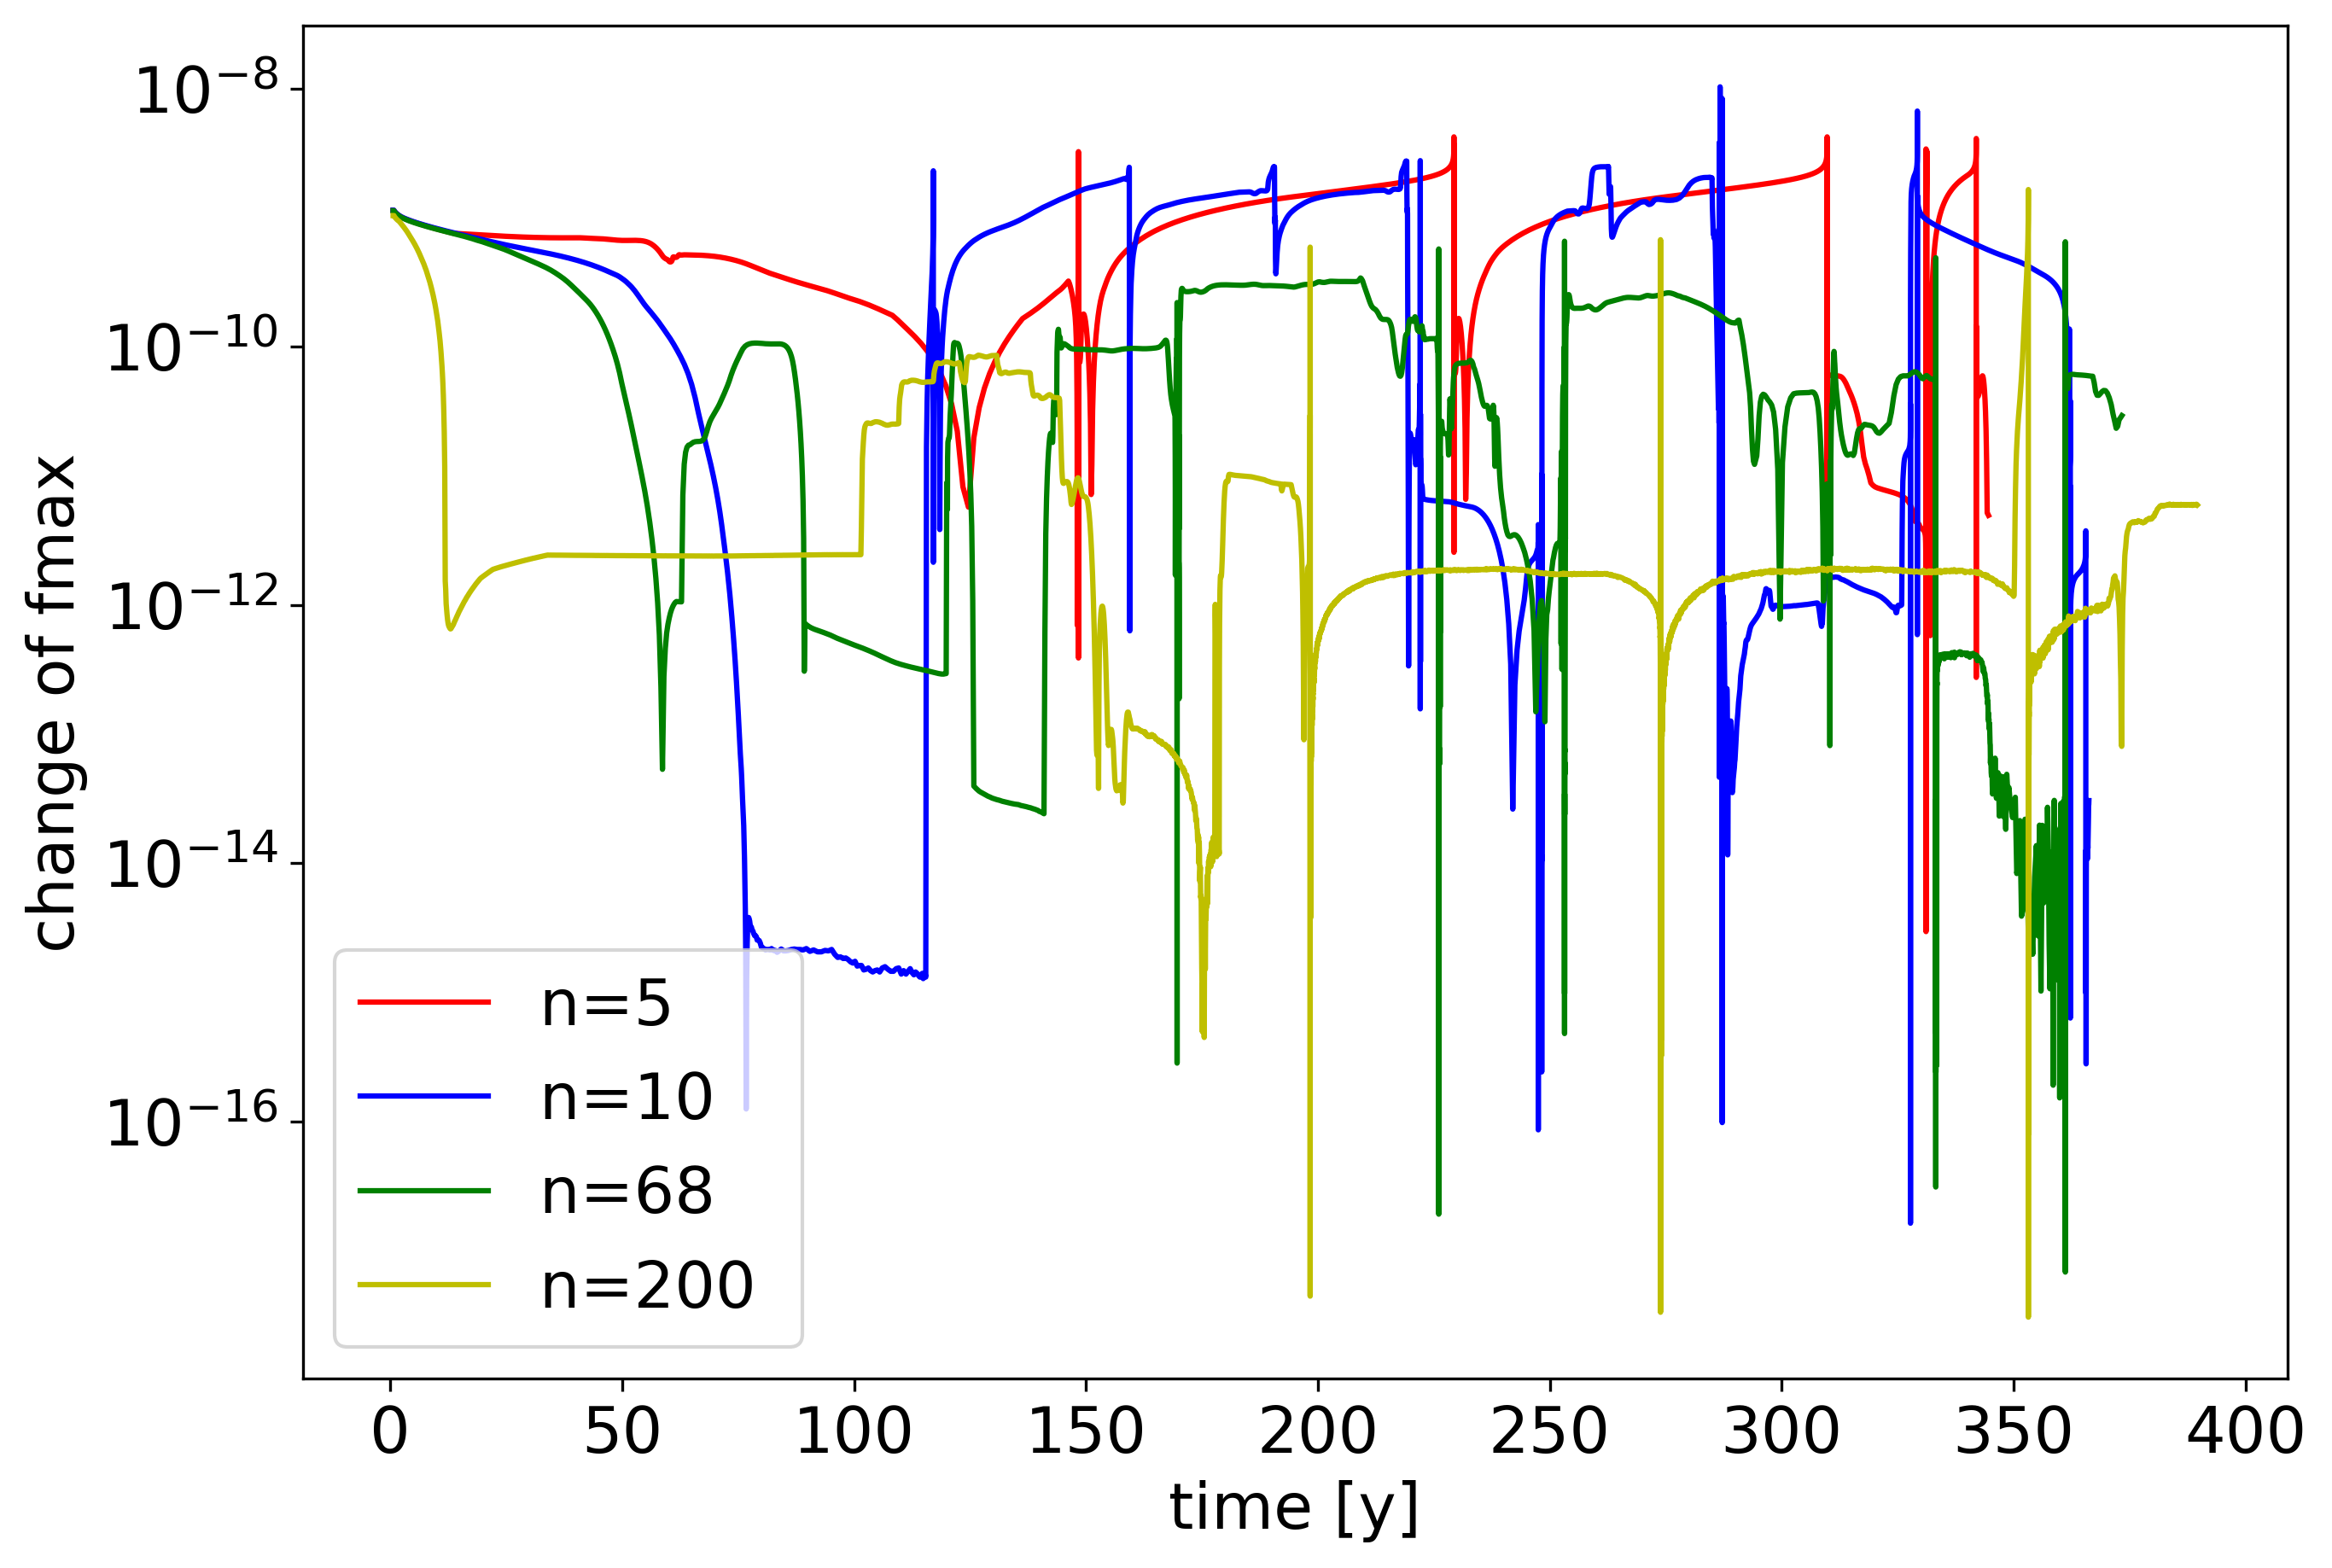
\includegraphics[width=1\textwidth]{images/TANDEMtimeEvolutionFLTEExtendedODEDifferentSizes.png}
		\subcaption{Absolute change of the friciton law per timestep, averaged over 50 timesteps} 
		\label{fig:timeEvolution_LTE_2ndOrderODE_differentSizes}
	\end{subfigure}
	\caption{Evolution of the value of the friction law of the 2nd order formulation over 400 years with varying domain sizes, where $n$ denotes the number of fault elements}
\end{figure}

Overall, the evaluation of the friction law is a suitable estimate for the global error in the system. Over the course of time, its value increases step wise at each earthquake, but overall linearly, which is due to a regular local truncation error. The main driver of the LTE is the tolerance for the slip rate $V$, which has been introduced to the system along with the second order ODE formulation. The upper bound for the LTE is proportional to the chosen tolerance.

\subsection{Scalability}

\section{Relative and Absolute Tolerances}
--> put that in the numerics section


\subsection{Tolerance of the State Variable Dependent on the Slip}
Overall, the absolute error of the slip is inferior to the absolute error of the state variable. From a physical point of view, the slip is a relevant quantity to describe earthquakes whereas the state variable $\psi$ is only required to solve the DAE. Therefore, the absolute and relative tolerances are defined as external requirements for the slip only, and the tolerances for the state variable have to be chosen in a way to achieve the best numerical performance without loosing physical accuracy. In the following equations, we try to evaluate the highest acceptable tolerances for the state variable in function of the provided tolerances for the slip. The relation between $S$ and $\psi$ is described by the friction law in \autoref{eq:SEASDAE_frictionLaw}, which is evaluated at a constant velocity $V^*$. For a maximal absolute slip error $\epsilon_S^a$, the largest acceptable absolute error of the state variable $\epsilon_\psi^a$ can be calculated by equalizing the induced error in the friction law under constant velocity. 
\begin{align}
    f_{V^*}(S+\epsilon_S^a,\psi) - f_{V^*}(S,\psi) &= f_{V^*}(S,\psi+\epsilon_\psi^a) - f_{V^*}(S,\psi) \\
    \tau(U(S+\epsilon_S^a)) - \tau(U(S)) &= a \sigma_n \text{arsinh}\left(\frac{V^*}{2V_0}\right)\frac{1}{a}\left(e^{\frac{\psi+\epsilon_\psi^a}{a}} - e^{\frac{\psi}{a}}\right) \\
    \tau(B(S+\epsilon_S^a)) - \tau(BS) &= a \sigma_n \text{arsinh}\left(\frac{V^*}{2V_0}\right) e^{\frac{\psi}{a}}\left(e^{\frac{\epsilon_\psi^a}{a}} - 1\right)
\end{align}

As already discussed in the formulation of the Jacobian matrix, the displacement $U(S)$ is linear in $S$ and can therefore be expressed with the linear transformation matrix $B$ as $U(S) = BS$. Further transformations of the left side of the equation are performed in index notation, where $\mathbbm{1}$ denotes a vector in which all components are equal to one. 
\begin{align}
    (\nabla u(S))_{pq} =& \frac{1}{2}\left(D_{lpq}^0u_l^0 + D_{lpq}^1u_l^1\right) + c_0\left(E_{lq}^0u_l^0 - E_{lq}^1u_l^1 - f_q\right)n_{pq} \\ \nonumber
    (\nabla u(S + \epsilon_S^a))_{pq} =& \frac{1}{2}\left(D_{lpq}^0\left(u_l^0+ B_{lj}\mathbbm{1}_j\epsilon_S^a\right) + D_{lpq}^1\left(u_l^1+ B_{lj}\mathbbm{1}_j\epsilon_S^a\right)\right) \\ &+ c_0\left(E_{lq}^0\left(u_l^0+ B_{lj}\mathbbm{1}_j\epsilon_S^a\right) - E_{lq}^1\left(u_l^1+ B_{lj}\mathbbm{1}_j\epsilon_S^a\right) - f_q\right)n_{pq} \\
    (\nabla u(S + \epsilon_S^a))_{pq} - (\nabla u(S))_{pq} =& \left(\frac{1}{2}\left(D_{lpq}^0 + D_{lpq}^1\right) + c_0\left(E_{lq}^0 - E_{lq}^1\right)n_{pq}\right)B_{lj}\mathbbm{1}_j\epsilon_S^a \\
    \tau_p(B(S+\epsilon_S^a)) - \tau_p(BS) =& M_{rp}^{-1}e_{qr}^Tw_q\left((\nabla u(S + \epsilon_S^a))_{kq} - (\nabla u(S))_{kq}\right)n_{kq}
\end{align}
We can see that the error in $\tau$ does not depend on the slip $S$ anymore and is proportional to the absolute slip error $\epsilon_S^a$. We can thus define a matrix $C$ such that $\tau_p(B(S+\epsilon_S^a)) - \tau_p(BS) = C_{pj}\mathbbm{1}_j\epsilon_S^a$. The absolute error of the state variable is then directly proportional to $\epsilon_S^a$. 
\begin{align}
    \epsilon_\psi^a &= a\text{ln}\left(1+\frac{C_{pj}\mathbbm{1}_j}{a\sigma_n \text{arsinh}\left(\frac{V^*}{2V_0}\right)e^{\frac{\psi}{a}}}\epsilon_S^a\right) 
\end{align}
To provide an upper bound for $\epsilon_\psi^a$, the smallest value of the proportionality factor of $\epsilon_S^a$ has to be determined because the logarithm function is increasing and the smallest allowed value of the error is searched. For the numerator of the ratio, to calculate $\min_p\left|C_{pj}\mathbbm{1}_j\right|$ minimizes the ratio. Note that the matrix $C$ depends on the geometry so this term cannot be provided in general in beforehand but has to be chosen with respect to the used space discretization. To minimize the ratio, the terms on the denominator have to be maximized. Because the arsinh function increases monotonously, the choice of $V_{max}$ for the velocity component provides an appropriate upper bound. Similarly, $\psi$ should be replaced by an upper limit $\psi_{max}$. The value of the parameter $a$ depends on the fault location and varies between $a_{min}$ and $a_{max}$. It appears once at the beginning of the denominator, where its maximal value shall be chosen, and once in the exponential, where its minimal value is required. If all those values are plugged into the expression, the error in $\psi$ can be evaluated as following: 
\begin{equation}
    \epsilon_\psi^a = a_{min}\text{ln}\left( 1+\frac{\min_p\left|C_{pj}\mathbbm{1}_j\right|}{a_{max}\sigma_n \text{arsinh}\left(\frac{V_{max}}{2V_0}\right) e^{\frac{\psi_{max}}{a_{min}}}}\epsilon_S^a\right)
\end{equation}
The upper bounds for the velocity and for the state variable can be deduced by already obtained simulation results and an appropriate choice could be the values $V_{max} = 5.0ms^{-1}$ and $\psi_{max} = 0.85$. In the simulation settings, $a$ increases from $a_{min}=0.010$ at the surface to $a_{max}=0.025$ at high depths. With these values, all terms take reasonable values, except for the exponential $e^{\frac{\psi_{max}}{a_{min}}} = e^{85} \approx 8\cdot10^{36}$. In the vicinity of 1,  the logarithm can be approximated by a linear function with gradient 1. Under consideration of the initial factor $a_{min}$, the absolute error tolerance in $\psi$ has to be 38 magnitudes below the tolerance in the slip to prevent any additional error. Such a low tolerance is not achievable in any realistic scenario, so the state variable participates in making the simulation less accurate. When the tolerances for the state variable have to be set, and only an absolute tolerance for the slip is provided, it is the best to chose them as low as possible, and still the state variable will contribute to the error of the simulation. On the other hand, very low tolerances prevent the choice of larger timesteps and an appropriate choice of the tolerance for the state variable which is not too low to ensure reasonable execution times still needs to be determined.  

\subsection{Tolerance of the State Variable Dependent on the Slip Rate}
So far, the error in the slip rate $V$ is not directly regulated by any tolerance value. Since it is calculated from the slip and from the state variable, the error in $V$ depends on the chosen tolerances for those two parameters. As a physical quantity, it might be interesting to provide a tolerance for the slip rate too. Unlike for the slip, the tolerance for the slip rate should also include a relative error tolerance $t_V^r$ in addition to the already discussed absolute error tolerance $t_V^a$. Indeed, the slip rate takes values around $10^{-6}ms^{-1}$ in the aseismic phase and peaks at values above $10^{9}ms^{-1}$ during the earthquake event. The exclusive use of an absolute error tolerance, with a value below the slip rate of the aseismic evolution, is too restrictive during the earthquake. An appropriate relative error tolerance, which is scaled by the current velocity value and added to the absolute one can reasonably restrict the error. In the aseismic phase, the relative error tolerance does not have much effect since it is scaled down by the very low slip rate and outmatched by the presumably higher absolute tolerance. For example, the choices $t_V^a=10^{-10}$ and $t_V^r=10^{-7}$ allow for a relative error of the order $10^{-4}$ during the aseismic phase and of the order $10^{-7}$ during the earthquake. Such a choice reflects the concept that a higher accuracy is needed to simulate an earthquake than to simulate aseismic slip. \\
The typical approach would be to estimate it with the difference between the values obtained from the numerical solution and its embedded solution. The newly chosen timestep shall then only allow solutions which fulfill the tolerances in the entire state vector and the additional tolerance in error of the slip rate. Alternatively, the error tolerance of the state variable, which is not properly defined from physical constrains yet can be used to restrict the slip rate. To obtain the relation between error in slip rate $V$ and state variable $\psi$, the same analysis as in the previous subsection has to be performed. This time, the error in the friction law is evaluated under the assumption of a constant slip $S^*$.  
\begin{align}
	f_{S^*}(V+\epsilon_V^a,\psi) - f_{S^*}(V,\psi) &= f_{S^*}(V,\psi+\epsilon_\psi^a) - f_{S^*}(V,\psi) \\
	 f_{S^*}(V,\psi) + \frac{d}{dV}f_{S^*}(V,\psi)\epsilon_V^a - f_{S^*}(V,\psi) + \mathcal{O}\left(\left(\epsilon_V^a\right)^2\right)&= a \sigma_n \text{arsinh}\left(\frac{V}{2V_0}\right)\frac{1}{a}\left(e^{\frac{\psi+\epsilon_\psi^a}{a}} - e^{\frac{\psi}{a}}\right) \\
	 \left( \frac{a\sigma_ne^{\frac{\psi}{a}}} {2V_0\sqrt{\left(\frac{V}{2V_0}\right)^2+1}}- \eta \right)\epsilon_V^a + \mathcal{O}\left(\left(\epsilon_V^a\right)^2\right) &= a \sigma_n \text{arsinh}\left(\frac{V}{2V_0}\right) e^{\frac{\psi}{a}}\left(e^{\frac{\epsilon_\psi^a}{a}} - 1\right)
\end{align}
\begin{equation}
	 \epsilon_\psi^a 
	= a\text{ln}\left(1 + \left( \frac{1}{\text{arsinh}\left(\frac{V}{2V_0}\right)\sqrt{V^2 + (2V_0)^2}} - \frac{\eta}{a \sigma_n \text{arsinh}\left(\frac{V}{2V_0}\right) e^{\frac{\psi}{a}}} \right)\epsilon_V^a + \mathcal{O}\left(\left(\epsilon_V^a\right)^2\right)\right)
\end{equation}
The exponential $e^{\frac{\psi}{a}}$ with the extremely high value appears again in one of the two ratios. The term with $\eta$ can thus be neglected to estimate the error. In the remaining summand, an appropriate estimate value for the slip rate $V$ needs to be determined. As stated previously, the absolute error tolerance is only relevant for the aseismic phase, in which the slip rate never exceeds the tectonic slip $V_0$, which can be taken as an upper bound for the slip rate here. The absolute error is then calculated by: 
\begin{equation}
	\label{eq:absoluteErrorPSIFromV}
	 \epsilon_\psi^a 
	= a_{min}\text{ln}\left(1 +  \frac{1}{\text{arsinh}\left(\frac{1}{2}\right)\sqrt{5}V_0}\epsilon_V^a\right)
\end{equation}
During an earthquake, the relative error tolerance of the slip rate is relevant. To evaluate it, we now investigate the relation between the relative errors of the slip rate and the state variable. 
\begin{align}
	f_{S^*}((1+\epsilon_V^r)V,\psi) - f_{S^*}(V,\psi) &= f_{S^*}(V,(1+\epsilon_\psi^r)\psi) - f_{S^*}(V,\psi) \\
	f_{S^*}(V,\psi) + \frac{d}{dV}f_{S^*}(V,\psi)\epsilon_V^rV - f_{S^*}(V,\psi) + \mathcal{O}\left(\left(\epsilon_V^rV\right)^2\right)&= a \sigma_n \text{arsinh}\left(\frac{V}{2V_0}\right)\frac{1}{a}\left(e^{\frac{(1+\epsilon_\psi^r)\psi}{a}} - e^{\frac{\psi}{a}}\right) \\
	\left( \frac{a\sigma_ne^{\frac{\psi}{a}}} {2V_0\sqrt{\left(\frac{V}{2V_0}\right)^2+1}}- \eta \right)\epsilon_V^rV + \mathcal{O}\left(\left(\epsilon_V^rV\right)^2\right) &= a \sigma_n \text{arsinh}\left(\frac{V}{2V_0}\right) e^{\frac{\psi}{a}}\left(e^{\frac{\epsilon_\psi^r}\psi{a}} - 1\right)
\end{align}
\begin{equation}
	\epsilon_\psi^r = \frac{a}{\psi}\text{ln}\left(1 + \left( \frac{1}{\text{arsinh}\left(\frac{V}{2V_0}\right)\sqrt{V^2 + (2V_0)^2}} - \frac{\eta}{a \sigma_n \text{arsinh}\left(\frac{V}{2V_0}\right) e^{\frac{\psi}{a}}} \right)\epsilon_V^rV + \mathcal{O}\left(\left(\epsilon_V^rV\right)^2\right)\right)
\end{equation}
Again, the term with $\eta$ can be neglected because of the exponential. For elements, where the relative tolerance is relevant, the slip rate is much larger than the tectonic slip, so $V_0^2$ can also be neglected below the square root when added to $V^2$. The relative error in $\psi$ can be estimated as: 
\begin{equation}
	\label{eq:relativeErrorPSIFromV}
	\epsilon_\psi^r = \frac{a_{min}}{\psi_{max}}\text{ln}\left(1 + \frac{1}{\text{arsinh}\left(\frac{V_{max}}{2V_0}\right)}\epsilon_V^r\right)
\end{equation}

The absolute and relative errors in $\psi$ associated to the respective errors in the slip rate are represented in \autoref{fig:RelAbsErrorToleranceVPSI}. The curves show the evaluation of \autoref{eq:absoluteErrorPSIFromV} and \autoref{eq:relativeErrorPSIFromV} for small error values in $V$. The various parameters are set to $a_{min}=0.01$, $\psi_{max}=0.85$, $V_0=10^{-6}ms^{-1}$ and $V_{max}=5.0ms^{-1}$. To use the previous example again, if an absolute error tolerance in the slip rate of $t_V^a=10^{-10}$ and a relative tolerance of $t_V^r=10^{-7}$ are required, it would translate to the tolerances in the state variable to $t_\psi^a=9.29\cdot10^{-7}$ and $t_\psi^r=2.77\cdot10^{-11}$. However, these values cannot be used as such in the simulation, since the assumption that the absolute tolerance can be neglected during the earthquake and inversely that the relative tolerance is insignificant in the aseismic phase only holds for the slip rate but not for the state variable, whose value remains between $0.75$ and $0.85$. It makes more sense to define an absolute tolerance for the aseismic slip $t_\psi^{as}=9.29\cdot10^{-7}$ and for the earthquake $t_\psi^{eq}=\psi_{min}2.77\cdot10^{-11}=6.48\cdot10^{-11}$ in the state variable. 

\begin{figure}[H]
	\centering
	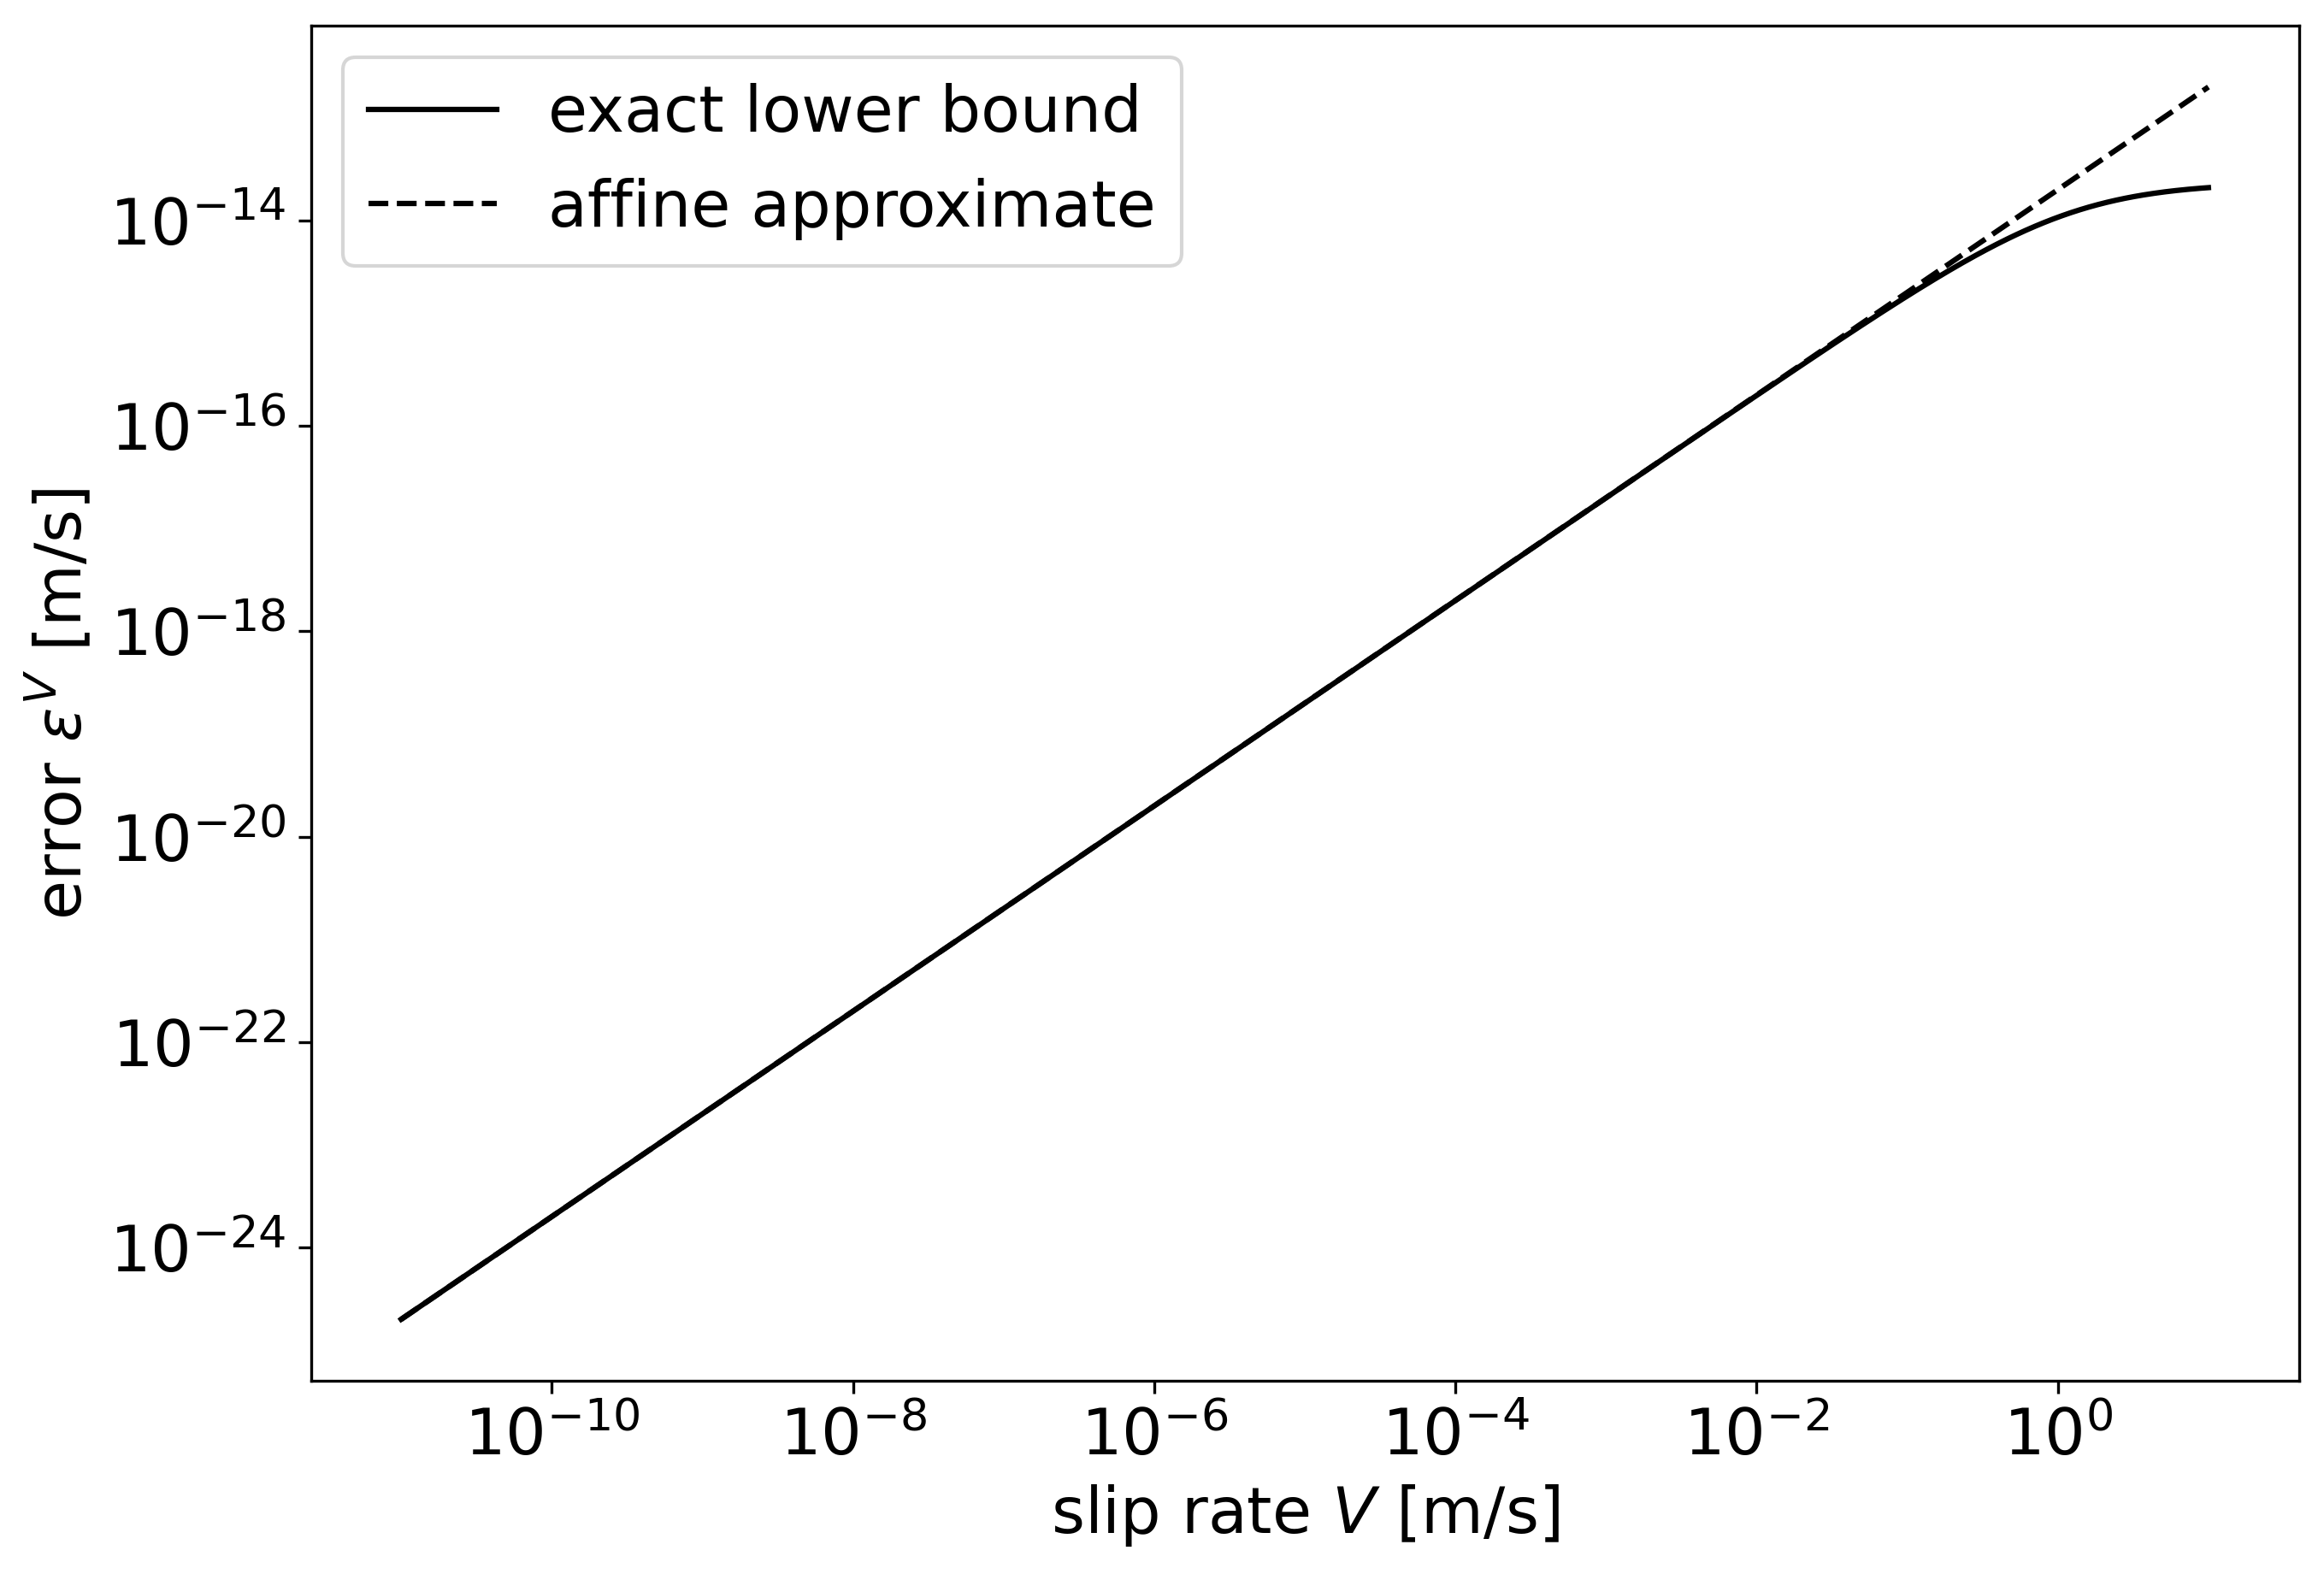
\includegraphics[width=0.6\textwidth]{images/ErrorRelationPSI_VAbsoluteRelative.png}
	\caption{Absolute and relative error in $\psi$ in function of the error in the slip rate}
	\label{fig:RelAbsErrorToleranceVPSI}
\end{figure}



\chapter{Four Formulations of the SEAS Problem}
\label{chap:44rmulations4SEAS}
Different approaches for solving the 2D antiplane shear problem are possible. First, four formulations of the SEAS problem are provided along with their analytic Jacobian matrices. Two of them are fully implicit and allow only implicit time integration methods whereas the two others allow for both explicit and implicit methods. This presentation is followed by a discussion about numerical and computational aspects of the four formulations with a major focus on the efficiency of the Newton iteration needed for solving implicit methods.

\section{First order formulations}
\label{sec:44mul4SEAS__1stOrderODE}
Three out of the four formulations are of first order, which means that at most the first time derivative of the physical quantities $S$ and $\psi$ appears. The first formulation in \autoref{ssec:444SEAS__1stOrderODE} can be solved explicitly and was the only originally available whereas the formulations in \autoref{ssec:444SEAS__extendedDAE} and \autoref{ssec:444SEAS__compactDAE} are purely implicit. All analytic Jacobian matrices in this section have been derived in the scope of this thesis.

\subsection{Formulation as a first order ODE}
\label{ssec:444SEAS__1stOrderODE}
\subsubsection{Problem}
The first approach to solve the SEAS problem is to formulate the system as a classical ODE. The solution vector contains the values for the slip and the state variable. At each timestep, the slip rate $V$ is calculated from the friction law $F$ with the bisection method and the time derivative of the state $\dot{\psi}$ can be directly calculated from the ageing law $G$, both in \autoref{eq:DAEFormulation2DSEAS}. The friction law is continuously differentiable and its Jacobian matrix with respect to $V$ in \autoref{eq:partial_df_dV} is invertible, with $i$ the index of each of the $n$ fault nodes. Therefore the implicit function theorem can be applied and states that a solution $V$ exists in $\mathbbm{R}^n$ where $V_i(S,\psi)$ is a continuously differentiable function. This approach was the only originally available implementation in {\ttfamily tandem}.

\begin{align}
	\label{eq:ODE_formulation_SEAS}
	x &= \begin{pmatrix}
		S \\ \psi
	\end{pmatrix} & \dot{x} &= \begin{pmatrix}
								  \dot{S} \\ \dot{\psi}
							   \end{pmatrix} = \begin{pmatrix}
												   V(S,\psi) \\ G(\psi, V)
											   \end{pmatrix} = \Gamma
\end{align} 

This formulation allows us to use many well-known and proven implicit and explicit numerical schemes. 

\subsubsection{Jacobian matrix}
\label{sssec:Jacobian_ODE}
For the ODE formulation in \autoref{eq:ODE_formulation_SEAS} it is not straightforward to calculate the Jacobian matrix because of the implicit evaluation of the slip rate $V$. At each fault node the right-hand side $\Gamma_i$ contains one component for each $V_i$ and $G_i$ and the solution vector $x_i$ one component for each $S_i$ and $\psi_i$. Therefore, four Jacobian matrices of size $\mathbbm{R}^{n\cross n}$ are needed to describe the system for each combination of the components in $\Gamma$ and $x$. They can be assembled to one general Jacobian matrix $\mathbf{J}_\Gamma$ of size $\mathbbm{R}^{2n\cross 2n}$ with four block matrices:
\begin{equation}
\label{eq:Jacobian_ODE_formulation}
\mathbf{J}_\Gamma(S,\psi,V)_{ij} = \begin{pmatrix} 
\pdv{V_i}{S_j} &
\pdv{V_i}{\psi_j} \\ 
\pdv{G_i(\psi,V)}{S_j} &
\pdv{G_i(\psi,V)}{\psi_j}  \end{pmatrix}
\end{equation}
In a first step, the partial derivatives of the slip rate $V$ will be calculated. The second part of the implicit function theorem provides an expression for the Jacobian matrices with respect to $S$ and $\psi$:
\begin{align}
\label{eq:partial_V_S}
\pdv{V_i}{S_j} &= -\left(\pdv{F}{V}\right)_{ik}^{-1}\pdv{F_k}{S_j} \\ 
\label{eq:partial_V_psi}
\pdv{V_i}{\psi_j} &= -\left(\pdv{F}{V}\right)_{ik}^{-1}\pdv{F_k}{\psi_j}
\end{align}
Two of the occurring matrices can be easily calculated from the analytic expression of the friction law in \autoref{eq:DAEFormulation2DSEAS}. A generalized Kronecker delta $\delta_{ij}^k$ is defined as 1 if $i=j=k$ and 0 otherwise.
\begin{align}
\pdv{F_i(S,\psi,V)}{\psi_j} &= \left( -\frac{\sigma_n}{2V_0} \frac{Ve^{\frac{\psi_k}{a}}}{\sqrt{\frac{e^{\frac{2\psi_k}{a}}V_k^2}{4V_0^2}+1}}\right)\delta_{ij}^k 
\label{eq:partial_df_dpsi} \\
\pdv{F_i(S,\psi,V)}{V_j} &= \left( -\frac{a\sigma_n}{2V_0} \frac{e^{\frac{\psi_k}{a}}}{\sqrt{\frac{e^{\frac{2\psi_k}{a}}V_k^2}{4V_0^2}+1}}-\eta\right)\delta_{ij}^k 
\label{eq:partial_df_dV}
\end{align}
Since $\pdv{F}{V}$ is a diagonal matrix, its inverse is very easy to calculate and does not require us to solve a linear system of equations. \\
The third derivative $\pdv{F}{S}$ is more complicated to obtain. In the friction law, $S$ appears only in the expression of the traction term $\tau$, so $\pdv{F}{S}=\dv{\tau}{S}$. As shown in \autoref{apx:dtau_dS}, it is a constant dense matrix. To precompute it, the computationally expensive DG problem needs to be solved $n$ times, where $n$ is the number of fault nodes. \\

To express the full Jacobian matrix of the ODE in \autoref{eq:Jacobian_ODE_formulation}, the partial derivatives of the ageing law $G$ are also required. They can be expressed in term of the already known partial derivatives: 
\begin{align}
	\pdv{G_i}{S_j}    &= -\frac{b}{L}\pdv{V_i}{S_j} \\
	\pdv{G_i}{\psi_j} &= -\frac{V_0}{L}e^{\frac{f_0 - \psi_k}{b}}\delta_{ij}^k -
						  \frac{b}{L}\pdv{V_i}{\psi_j}
\end{align}



\subsection{Formulation as a DAE}
\label{ssec:444SEAS__extendedDAE}
\subsubsection{Problem}
The ODE form may not be ideal because of the implicit evaluation of the slip rate, which is treated independently of the numerical integration. Alternatively, the friction law could be solved for the slip rate together with $S$ and $\psi$. The solution vector is then extended by one quantity and $V$ is not evaluated with a separate iterative scheme anymore.
\begin{align}
	\label{eq:DAE_formulation_SEAS}
	x &= \begin{pmatrix}
			S \\ \psi \\ V
		 \end{pmatrix} & \dot{x} &= \begin{pmatrix}
										\dot{S} \\ \dot{\psi} \\ 0
									\end{pmatrix} = \begin{pmatrix}
										V \\ G(\psi, V) \\ F(S,\psi,V)
									\end{pmatrix}
\end{align}
This formulation necessarily requires an implicit time integration method which iteratively solves for the time-variant quantities $S$ and $\psi$ as well for the algebraic state $V$. The main difference to the ODE formulation with an implicit method is the sparser structure of the Jacobian matrix. The arising linear system can be solved more efficiently with direct and iterative solvers as it will be discussed in detail in \autoref{ssec:iterative_solver_Jacobian}. \\
The PETSc interface requires us to provide a DAE in the form
\begin{align}
	\Phi(t, x,\dot{x}) = \Gamma(t,x) 
\end{align}
where the left-hand side function $\Phi$ depends on the solution vector and its time derivative whereas the right-hand side function $\Gamma$ only depends on the solution vector. For now, we choose a fully implicit formulation of the problem, in which $\Gamma$ vanishes. The DAE can then be expressed in the following way: 
\begin{align}
\label{eq:DAE_extended_formulation_SEAS}
	x &= \begin{pmatrix}
		S \\ \psi \\ V
	\end{pmatrix} & \Phi(t, x,\dot{x}) &= \begin{pmatrix}
	 	V - \dot{S} \\ G(\psi, V) - \dot{\psi}  \\ F(S,\psi,V)
	\end{pmatrix} = \begin{pmatrix}
		0 \\ 0 \\ 0
	\end{pmatrix} = \Gamma(t,x)
\end{align}

Another class of solvers, the so-called IMEX (implicit-explicit) solvers \cite{IMEX}, offer an interesting approach to numerically solve this problem, by mixing an implicit, iterative method for the algebraic states with an explicit method for the remaining simple time-dependent quantities. Technically, the function $\Phi$ is expected to be integrated implicitly, while the right-hand side function $\Gamma$ is solved explicitly. In the given formulation, we could shift the time derivatives of $S$ and $\psi$ to the right-hand side of the equation. This approach is not further considered in this thesis, but might be worth looking at in future work.

\subsubsection{Jacobian matrix}
\label{sssec:Jacobian_DAE}
For the DAE formulation of the system in \autoref{eq:DAE_extended_formulation_SEAS}, another approach can be chosen to calculate the Jacobian matrix of the system. With now three different components in the solution vector, the Jacobian matrix contains the partial derivatives with respect to the slip rate in addition to the slip and to the state variable. Similarly, the function $\Phi$ on which the Jacobian is applied is extended by the friction law. Each block $(i,j)$ in the structure of the Jacobian is given by:
\begin{equation}
\label{eq:Jacobian_DAE_formulation}
\mathbf{J}_\Phi(S,\psi,V)_{ij} = \begin{pmatrix}
\pdv{V_i}{S_j} & \pdv{V_i}{\psi_j} & \pdv{V_i}{V_j} \\
\pdv{G_i(\psi,V)}{S_j} & \pdv{G_i(\psi,V)}{\psi_j} & \pdv{G_i(\psi,V)}{V_j} \\
\pdv{F_i(S,\psi,V)}{S_j} & \pdv{F_i(S,\psi,V)}{\psi_j} & \pdv{F_i(S,\psi,V)}{V_j}
\end{pmatrix}
\end{equation}
In the previous section, a complicated approach had to be followed to obtain the derivative for the slip rate because of the nonlinear friction law, which was indirectly solved for each evaluation of the slip rate. Since the slip rate is now obtained directly from the solution vector $x$ and not from an iterative solver for the friction law, all its partial derivatives except with each component itself vanish. 

\begin{align}	
\pdv{V_i}{S_j} &= 0 & \pdv{V_i}{\psi_j} &= 0 & \pdv{V_i}{V_j} &= \delta_{ij}
\end{align}

Similarly, the partial derivatives of the ageing law can be directly evaluated from its definition in \autoref{eq:DAEFormulation2DSEAS}.
\begin{align}
\pdv{G_i(\psi,V)}{S_j} &=  0 &
\pdv{G_i(\psi,V)}{\psi_j} &= -\frac{V_0}{L}e^{\frac{f_0-\psi_k}{b}}\delta_{ij}^k &	
\pdv{G_i(\psi,V)}{V_j} &= -\frac{b}{L} \delta_{ij}
\end{align}
For the friction law, the Jacobian matrices have already been calculated in \autoref{eq:partial_df_dpsi} for $\pdv{F(S,\psi,V)}{\psi}$, in \autoref{eq:partialDerivative_df_dS} for $\pdv{F(S,\psi,V)}{S}$ and in \autoref{eq:partial_df_dV} for $\pdv{F(S,\psi,V)}{V}$.

This formulation of the Jacobian cannot be directly used in the Newton iteration to calculate the next timestep. Typically, the Jacobian has to be adapted to represent the time-stepping scheme. For instance, the implicit Euler method results requires to solve the nonlinear equation $0 = 1/h(x_n - x_{n+1}) + F(x_{n+1})$ for the solution at the next timestep $x_{n+1}$ and the Jacobian matrix $J_N$ for the corresponding Newton iteration is constructed from $J$. 
\begin{equation}
J_N = -\frac{1}{h}I + J
\end{equation}
Here, the problem arises that the time evolution is only defined for two components in the solution vector: the slip $S$ and the state variable $\psi$. The slip rate $V$ needs to be solved algebraically at every Newton iteration, but this component should not be included in the time-stepping scheme. The nonlinear equation to calculate a step of the implicit Euler has to be adapted to include properly the slip rate. 
\begin{align}
0 = \begin{pmatrix} \frac{1}{h}S_n     \\ \frac{1}{h}\psi_n     \\ 0 \end{pmatrix} - 
\begin{pmatrix} \frac{1}{h}S_{n+1} \\ \frac{1}{h}\psi_{n+1} \\ 0 \end{pmatrix} + 
\begin{pmatrix} V_{n+1}            \\ g(\psi_{n+1},V_{n+1}) \\ f(S_{n+1}, \psi_{n+1}, V_{n+1}) \end{pmatrix}
\end{align}
The Jacobian matrix to be used in a Newton iteration to solve this problem has to be changed accordingly.
\begin{align}
\label{eq:Jacobian_Newton_Iteration_extended_DAE}
\mathbf{J}_N = 
\begin{pmatrix} 
-\frac{1}{h}\mathbf{I} & \mathbf{0}            & \mathbf{0} \\ 
\mathbf{0}             &-\frac{1}{h}\mathbf{I} & \mathbf{0} \\ 
\mathbf{0}             & \mathbf{0}            & \mathbf{0} 
\end{pmatrix} + 
\begin{pmatrix}  
\mathbf{J}_S(S)    &  \mathbf{J}_\psi(S)    &  \mathbf{J}_V(S)    \\ 
\mathbf{J}_S(\psi) &  \mathbf{J}_\psi(\psi) &  \mathbf{J}_V(\psi) \\ 
\mathbf{J}_S(V)    &  \mathbf{J}_\psi(V)    &  \mathbf{J}_V(V)
\end{pmatrix} =
\begin{pmatrix} 
-\frac{1}{h}\mathbf{I}         &  \mathbf{0} 			            &
\mathbf{I}                     \\ 
\mathbf{0}                    & 
-\frac{1}{h}\mathbf{I} +  \pdv{g}{\psi}       &  \pdv{g}{V} \\ 
\pdv{f}{S} & \pdv{f}{\psi} &  \pdv{f}{V} 
\end{pmatrix}
\end{align}
If other implicit numerical schemes are used than the implicit Euler, such as higher-order BDF methods, $\mathbf{J}_N$ can be easily changed by multiplying the identity matrices $\mathbf{I}$ with a coefficient that depends on the chosen method. Albeit this formulation of the Jacobian matrix is perfectly valid, it is very specific to the SEAS problem and is therefore hard to implement as such within the PETSc framework. \\
To solve general implicit DAEs of the form $\Phi(t,x,\dot{x}) = \Gamma(t,x)$, PETSc offers a convenient interface to provide the Jacobian matrices. In fact, three matrices have to be provided. The first Jacobian matrix, denoted by $\bm{\Gamma}_{\dot{x}}$, corresponds to the variation of the left-hand side function $\Phi$ with respect to the derivative of the solution vector. The second matrix $\bm{\Gamma}_x$ describes the variation of the same function under the actual solution vector. Finally, the third Jacobian matrix $\bm{\Gamma}_x$ represents the variation of the right-hand side function $\Gamma$ under the influence of $x$. In our case, the formulation is fully explicit and the right hand side function $\Gamma(t,x)$ is zero everywhere, and by extension, its Jacobian matrix $\bm{\Gamma}_x$ also vanishes. It remains to express the Jacobian matrix of the Newton iteration $\mathbf{J}_N$ in terms of $\bm{\Phi}_x$ and $\bm{\Phi}_{\dot{x}}$:
\begin{equation}
\mathbf{J}_N = \frac{d\Phi}{dx_n} = \bm{\Phi}_{\dot{x}}\frac{d\dot{x}_n}{dx_n} + \bm{\Phi}_x	
\end{equation}
The term $\frac{d\dot{x}_n}{dx_n}$ is a scalar and depends only on the chosen timestep scheme, which can be denoted by $\sigma$. For the implicit Euler method for instance, we have $\sigma = 1/h$. The Jacobian matrix $\bm{\Phi}_x$ is exactly the one expressed in \autoref{eq:Jacobian_DAE_formulation} and $\bm{\Phi}_x$ contains negative identity matrices at the entries for the slip $S$ and for the state variable $\psi$.
\begin{align}
\bm{\Phi}_x = \begin{pmatrix} 
\mathbf{0}                     &  \mathbf{0}                       & 
\mathbf{I}                    \\ 
\mathbf{0}                     &  \pdv{G}{\psi} & 
\pdv{G}{V} \\ 
\pdv{F}{S}  &  \pdv{F}{\psi} &  
\pdv{F}{V} 
\end{pmatrix} &&&
\bm{\Phi}_{\dot{x}} = \begin{pmatrix} 
-\mathbf{I}  &  \mathbf{0}  & \mathbf{0} \\ 
\mathbf{0}  & -\mathbf{I}  & \mathbf{0} \\ 
\mathbf{0}  &  \mathbf{0}  & \mathbf{0}
\end{pmatrix}
\end{align}
With these two matrices, the Jacobian matrix for the Newton iteration of the implicit Euler method is the same as calculated in \autoref{eq:Jacobian_Newton_Iteration_extended_DAE}.



\subsection{Compact formulation as a DAE}
\label{ssec:444SEAS__compactDAE}
\subsubsection{Problem}
It is important to remember that the slip rate is the time derivative of the slip, so the variables $\dot{S}$ and $V$ are equal and can be interchanged in the problem formulation. As such, the friction law can be solved directly for $\dot{S}$ and the term $V$ is not required anymore. The solution vector then remains with the components of the slip $S$ and of the state variable $\psi$, as previously in the ODE formulation.
 \begin{align}
	\label{eq:DAE_compact_formulation_SEAS}
	x &= \begin{pmatrix}
			S \\ \psi
	     \end{pmatrix} & \Phi(t, x,\dot{x}) &= \begin{pmatrix}
												F(S,\psi,\dot{S}) \\ G(\psi, \dot{S}) - \dot{\psi}
											\end{pmatrix} = \begin{pmatrix}
																0 \\ 0
															\end{pmatrix} = \Gamma(t,x)
\end{align}
As in the previous DAE formulation, the friction law is solved along with time-variant quantities $S$ and $\psi$. Therefore it can be only used with an implicit integrator. \\

\subsubsection{Jacobian matrix}
The compact DAE formulation of the problem in \autoref{eq:DAE_compact_formulation_SEAS} also requires to be solved fully implicitly and involves again the three Jacobian matrices, $\mathbf{F}_{\dot{x}}$, $\mathbf{F}_x$ and $\mathbf{G}_x$, where the last one also vanishes because the right-hand side function is zero. The block matrices that appear in this formulation are calculated in the same way as previously but are arranged differently.
\begin{align}
	\label{eq:Jacobian_compact_DAE}
	\bm{\Phi}_{\dot{x}}&=  \begin{pmatrix}
								\pdv{F}{V} &  \mathbf{0} \\
							    \pdv{G}{V} & -\mathbf{I}
							\end{pmatrix} & 
	\bm{\Phi}_x        &=  \begin{pmatrix}
								\pdv{F}{S} & \pdv{F}{\psi} \\
								\mathbf{0} & \pdv{G}{\psi}
							\end{pmatrix} & 
	\bm{\Gamma}_x        &=  \begin{pmatrix}
								\mathbf{0} & \mathbf{0} \\
							    \mathbf{0} & \mathbf{0}
							\end{pmatrix}
\end{align}

\subsection{Verification of the Jacobian matrices}
All Jacobian matrices defined in this section have been checked for correctness. For that, a second order central finite difference approximation \cite[p. 184]{introductionPartialDiffEquations} is used to approximate each term of the Jacobian. 
\begin{equation}
	\mathbf{J}_{ij} = \pdv{\Phi_i}{x_j} \approx \frac{\Phi_i(x + he_j) - \Phi_i(x - he_j)}{2h}
\end{equation}
The function $F$ has to be evaluated $2n$ times with the current solution vector $x$ and a variation $h$ applied in positive and negative direction to each component of $x$ respectively. For this, the function to evaluate the right-hand side of the ODE or respectively the left-hand side for the DAEs is called. For an appropriate choice of $h$, not too large to be accurate and not too small to avoid truncation errors, the relative error between the analytic expression of the Jacobian and its approximation is inferior to $10^{-5}$ in all components and therefore, the expressions for the Jacobian matrices can be considered to be correct.

\subsection{Practical limitations of the Jacobian matrices}
The main advantage of implicit methods over explicit methods is to allow larger timesteps without accuracy loss. The program execution is therewith expected to be accelerated. The proposed calculation of the Jacobian matrix and its application in Newton iterations comes along with some drawbacks concerning the required calculation effort. \\
As described in \autoref{sssec:Jacobian_ODE}, the computation of the Jacobian matrix can be split up in one constant part $\pdv{\tau}{S}$ that has to be evaluated once at the beginning of the simulation and only depends on the domain geometry and in one variable part, that needs to be updated after each evaluation of the solution vector $x_n$. The initialization can be quite computationally expensive, as it requires, for each column of $\pdv{\tau}{S}$, to solve the Discontinuous Galerkin system for the entire domain with the corresponding unit vector as right-hand side vector. Each calculation of this linear system is approximately as expensive as performing one timestep with an explicit solver, since solving the same linear system is the most expensive operation of a timestep. For large domains with several hundred or thousand fault elements, which each contains a couple of fault nodes, this initialization operation takes a considerable amount of time. In comparison with an explicit scheme, a potential implicit method starts the race for the fastest solver with a penalty of about $n$ explicit timesteps, where $n$ is the total number of nodes on the fault. The advantages of implicit methods will therefore only pay off after a high number of iterations and make such methods of interest only if the simulated time frame is very long. This is typically the case because current simulations of sequences of earthquakes over several centuries with a high mesh resolution require up to a million timesteps with explicit methods. \\
Another potential drawback of the Newton method is that a linear system of size $n$ needs to be solved at each iteration step. This might still sound much less than solving for the displacement on the whole DG-domain of size $N$ as it is required to evaluate the right-hand side of the ODE at each iteration too. However, the DG system has a constant matrix $A$ whose LU-decomposition can be calculated once at the beginning of the simulation and each evaluation of the right-hand side only requires a backward substitution of complexity $\mathcal{O}\left(N^2\right)$. For the Jacobi matrix, such a pre-processing is not available since it changes along with the solution vector. Every calculation to solve the linear system in the Newton iteration is achieved with a complexity of the order $\mathcal{O}\left(n^3\right)$. In particular in large domains with many fault nodes, the solver with cubic complexity involves a substantially higher execution time than the one with quadratic complexity. 

\subsection{Iterative solvers for the Jacobian matrices}
\label{ssec:iterative_solver_Jacobian}
As discussed in the previous section, a linear system of equations has to be solved at each Newton iteration, and since the Jacobian matrices depend on the current solution vector, an expensive LU decomposition in $\mathcal{O}\left(n^3\right)$ has to be calculated at each step. This can be avoided with iterative solvers, which reduce the complexity of each Newton step to $\mathcal{O}\left(kn^2\right)$, where $k$ is the number of iterations in the matrix solver. \\
For the two DAE formulations, the partial sparse structure of the Jacobian matrix can be used to reformulate the system of equations in a way that iterative methods can be applied efficiently. We use the fact that among all submatrices, that are used to set up the Jacobian matrix, the only dense matrix is the constant term $\pdv{f}{S}$, and all other terms, are diagonal matrices. Let us consider the example of the Jacobian of the compact DAE formulation in \autoref{eq:Jacobian_compact_DAE}, with the linear system in which it appears in the Newton iteration. The dense term is denoted by the matrix $\mathbf{B}$ and all other block matrices $J_{ij}$ are diagonal.
\begin{equation}
	\begin{pmatrix}
		\mathbf{B} & \mathbf{J}_{12} \\ 
		\mathbf{J}_{21} & \mathbf{J}_{22} 
	\end{pmatrix} \begin{pmatrix}
		x_1 \\ x_2
	\end{pmatrix} = \begin{pmatrix}
		b_1 \\ b_2
	\end{pmatrix} 
\end{equation}
The vector $x$ describes the change in each component at the current Newton step and is the searched unknown and $b$ contains the left-hand side of the DAE system. Under the assumption that there are no zero entries on the diagonals, we first transform the Jacobian matrix to a lower triangular block matrix and obtain the following modified system: 
\begin{equation}
	\begin{pmatrix}
		\mathbf{B} - \mathbf{J}_{12}\mathbf{J}_{22}^{-1}\mathbf{J}_{21} & \mathbf{0} \\ 
		\mathbf{J}_{12} & \mathbf{J}_{22} 
	\end{pmatrix} \begin{pmatrix}
		x_1 \\ x_2
	\end{pmatrix} = \begin{pmatrix}
		b_1 - \mathbf{J}_{12}\mathbf{J}_{22}^{-1}b_2 \\ b_2
	\end{pmatrix} 
\end{equation}

Now, an iterative solver can be applied on the subsystem in the first line on the dense, but diagonally dominant to solve for the components in $x_1$. The components in $x_2$ can then be easily derived in $\mathcal{O}(n)$ operations with a forward substitution because all matrices $J_{ij}$ are diagonal. \\
A similar transformation was also obtained for the extended DAE formulation in \autoref{apx:ReducedJacobianExtendedDAE}, where the iterative solver is only required on a subsystem of size $n$ and where the missing components can be updated linearly in time. Without the reduction, no iterative methods with fast convergence could be found. For the first order ODE formulation, such a Gaussian elimination is not expedient because two out of the four submatrices are dense. However, iterative methods can directly be used on the entire Jacobian matrix.


\section{Second Order Differential Equation}
\label{sec:44mul4SEAS__2ndOrderODE}

So far, the original problem in \autoref{eq:DAEFormulation2DSEAS} has been formulated as a first order ODE in \autoref{eq:ODE_formulation_SEAS}, in which the friction law is solved implicitly within each evaluation of the right-hand side, such that explicit time integrators can be used. The solution vector has a compact size and only includes the slip $S$ and the state variable $\psi$. Alternatively, the problem can be directly formulated as a DAE, where the solution vector is extended by the slip rate $V$, such that it can be solved through the friction law iteratively together with the time quantities $S$ and $\psi$. A compact form of the DAE has also been formulated, where the derivative slip rate is directly used in the friction law instead of introducing a new variable~$V$. \\
The original motivation was to define an extended ODE formulation as counterpart to the extended DAE form, such that the solution vector contains an additional component for the slip rate $V$. To achieve this goal, it is necessary to find a function $H(t,S,\psi,V)$ which describes the change in time of the slip rate $\frac{dV}{dt}$. Since $V$ itself is the time derivative of the slip, this function $H$ corresponds to the second time derivative of the slip, or the slip acceleration. The new ODE formulation is: 
\begin{align}
&&	 x      =& \begin{pmatrix}	S                     \\ \psi           \end{pmatrix}      &
	 		   \begin{pmatrix}	\ddot{S}              \\ \dot{\psi}     \end{pmatrix}
			=& \begin{pmatrix}	H(t,S,\psi,\dot{S})   \\ G(\psi, V)     \end{pmatrix}
			 	 		 \\ &\Leftrightarrow&	 		  		 
	 x      =& \begin{pmatrix}	S       \\ \psi       \\ V	            \end{pmatrix}      &
   	\dot{x}  = \begin{pmatrix}	\dot{S} \\ \dot{\psi} \\ \dot{V}        \end{pmatrix}
	 		=& \begin{pmatrix}	 V      \\ G(\psi, V) \\ H(t,S,\psi,V)  \end{pmatrix}
	 		 = \Gamma	
	\label{eq:2nd_order_ODE_formulation}
\end{align}
Here, the friction law does not appear in the right-hand side anymore and is included in the function $H$. Unlike the previous ODE formulation, it does not require to solve the friction law implicitly at every timestep for the slip rate $V$ (or for any other quantity), therefore the new formulation is not a DAE anymore. Another beneficial advantage is, that if the boundary conditions of the DG domain are linear in time, it does not require solving the DG system at every timestep, which is the main performance bottleneck after initialization in the first order formulations. 

\subsection{Obtaining the second order ODE formulation}
This section will focus on the derivation of the right-hand side term $H(t,S,\psi,V)$, which is necessary to formulate the second order ODE. Starting point is the expression for the friction law in \autoref{eq:DAEFormulation2DSEAS}. At any time in the simulation, this algebraic equation always evaluates to zero, and therefore, its time derivative also vanishes. With the help of the formula of total derivatives, we obtain the following expansion: 
\begin{align}
	0 = \dv{F}{t} &= \pdv{F}{t} + \pdv{F}{S}\dv{S}{t} + \pdv{F}{\psi}\dv{\psi}{t} +  \pdv{F}{V}\dv{V}{t} \nonumber\\
					  &= \pdv{F}{t} + \pdv{F}{S}V + \pdv{F}{\psi}G(\psi,V) + \pdv{F}{V}H(t,S,\psi,V)
\end{align}
The partial derivatives of $F$ that occur are calculated in the same way as for the Jacobian matrices of the first order formulations. The terms $\pdv{F}{\psi}$ and $\pdv{F}{V}$ are diagonal matrices with the entries stated in \autoref{eq:partial_df_dpsi} and \autoref{eq:partial_df_dV} and the term $\pdv{F}{S}$ is a constant, full matrix which depends on the geometry of the domain and is derived in \autoref{eq:partialDerivative_df_dS}. None of these terms depends on the slip $S$ anymore, so $H$ can be calculated independently from $S$. After some transformations, it can be expressed as: 
\begin{equation}
	\label{eq:2nd_order_ODE_formulation_sum_of_Jacobians}
	H(t,\psi,V) = -\left(\pdv{F}{V}\right)^{-1}\left(\pdv{F}{t} + \pdv{F}{S}V + \pdv{F}{\psi}G(\psi,V)\right)
\end{equation}
It can be noted that this expression is very similar to the Jacobian matrix of the first order ODE formulation. If $x=(S,\psi)^T$ stands for its solution vector and $\mathbf{J}_{S}$ denotes the first row of block matrices of its Jacobian matrix in \autoref{eq:Jacobian_ODE_formulation}, an alternative definition of $H$ could be: 
\begin{equation}
	\label{eq:2nd_order_ODE_formulation_concise}
	H(t,\psi,V) = \mathbf{J}_{S}\dv{x}{t} -\left(\pdv{F}{V}\right)^{-1}\pdv{F}{t}
\end{equation}
The last missing term is the partial derivative of the friction law $F$ with respect to the time variable $t$. In its definition, the only component that directly depends on time is the traction $\tau$ through the boundary conditions of the DG domain. Typically, at boundary nodes that are not on the fault, the slip $S_b$ there is prescribed and evolves with time to represent the natural movement of the tectonic plate. For a constant environment slip rate $V_p$, we calculate $S_b=V_pt$ for the general case or $S_b=V_p/2\;t$ if the domain is symmetric. The boundary slip is linear in time, so its first derivative $\dot{S}_b$ will be constant. In the DG problem, boundary conditions are included in the right-hand side $b$ and contribute to the traction $\tau$ on the fault through linear transformations. To obtain $\pdv{\tau}{t}$ on the fault, it is then sufficient to solve the Poisson problem with only $\dot{S}_b$. Since this term is constant, $\pdv{F}{t}$ is also constant it is enough to solve the Poisson problem once at the beginning of the simulation and then, at each evaluation of the right-hand side of the ODE, use the same term $\pdv{F}{t}$. To reuse existent code structures, $\pdv{\tau}{t}$ can be pre-calculated with the DG solver for $\tau$ using a slip of 0 everywhere on the fault and by evaluating the boundary condition at the time $t=1$. \\
In comparison with the first order ODE formulation, the new second order formulation needs a considerable initialization phase but evaluates the right-hand side of the ODE much faster. In addition to the LU-decomposition of the DG matrix $A$, the initialization of the Jacobian $\pdv{F}{S}$ needs to solve the Poisson problem on the DG domain of size $N$ once per fault node, so in total $n$ times. Moreover, the problem needs to be solved once to calculate the initial condition of $V$ from the initial $S$ and $\psi$ and once to initialize the time derivative of the friction law $\pdv{F}{t}$. At each evaluation of the right-hand side of the first order ODE, the DG system needs to be solved with its LU-decomposition in $\mathcal{O}\left(N^2\right)$ and the remaining components of the vector set up in $\mathcal{O}\left(n^2\right)$ because of the matrix-vector product in $\tau$, so the total complexity is $\mathcal{O}\left(n^2+N^2\right)$. In contrast, the second order formulation only needs matrix-vector multiplications on the fault node, so its total complexity per evaluation is reduced to $\mathcal{O}\left(n^2\right)$. Since $n\ll N$, it is expected that the new formulation performs much better for long simulated times. \\
However, if the boundary conditions are not linear in time, the derivative $\pdv{\tau}{t}$ is not constant anymore and needs to be evaluated at every timestep. Therefore the solution of the Poisson problem is needed again at every timestep. The complexity increases back to $\mathcal{O}\left(n^2+N^2\right)$ and the main advantage of the second order formulation is lost. For now, we do not consider this case and always assume that the boundary conditions are linear in time.  \\

\subsection{Derivation of the analytic Jacobian}
The Jacobian of the second order ODE formulation in \autoref{eq:2nd_order_ODE_formulation} has components in the slip $S$, the state variable $\psi$ and in the slip rate $V$. The block structure is given by:
\begin{equation}
\label{eq:Jacobian_2nd_order_ODE_formulation}
	\mathbf{J}_\Gamma(S,\psi,V)_{ij} = 	\begin{pmatrix}
	\pdv{V_i}{S_j} 				& \pdv{V_i}{\psi_j}	 			& \pdv{V_i}{V_j} \\
	\pdv{G_i(\psi,V)}{S_j} 		& \pdv{G_i(\psi,V)}{\psi_j}	 	& \pdv{G_i(\psi,V)}{V_j} \\
	\pdv{H_i(t,\psi,V)}{S_j} 	& \pdv{H_i(t,\psi,V)}{\psi_j} 	& \pdv{H_i(t,\psi,V)}{V_j}
\end{pmatrix}
\end{equation}
It can be directly seen that none of the terms $V$, $G$ and $H$ depend on the slip $S$, therefore all entries in the first column of block matrices evaluate to 0. A direct consequence is the singularity of the Jacobian matrix, which makes it unsuitable for the Newton iteration. The Jacobian matrix takes the following form, where $\mathbf{K}$ is invertible with a partial diagonal structure:
\begin{align}
\label{eq:Jacobian_2nd_order_ODE_formulation_with_zeros}
\mathbf{J}_\Gamma(S,\psi,V)_{ij} &= 	\begin{pmatrix}
\mathbf{0} 												& \begin{matrix}\mathbf{0} & \mathbf{I} \end{matrix} \\
\;\,\begin{matrix}\mathbf{0} \\ \mathbf{0} \end{matrix} & \mathbf{K} 	\\
\end{pmatrix} & 
\mathbf{K} &= \begin{pmatrix}
	\pdv{G_i(\psi,V)}{\psi_j}	 	& \pdv{G_i(\psi,V)}{V_j} \\
	\pdv{H_i(t,\psi,V)}{\psi_j} 	& \pdv{H_i(t,\psi,V)}{V_j}
\end{pmatrix} 
\end{align} 

To cope with this issue, recall that $G$ and $H$ do not depend on $S$, it is thus possible to apply the Newton iteration only on $\psi$ and $V$ with the reduced Jacobian $\mathbf{K}$. Once the slip rate $V^{(n+1)}$ is known for the next timestep, the implicit scheme can be directly applied to $S$ without the need to solve a nonlinear system of equations. Indeed, the value of the right-hand side of the ODE at the next timestep for $\dot{S}^{(n+1)} = V^{(n+1)}$ is directly available and can be plugged in the BDF scheme. If $S^{(n-i)}$ are the solutions at the $i$ previous timesteps, $\alpha_{n-i}$ the time adaptive BDF coefficients at these steps and $\sigma$ the current shift, the new slip rate $S^{(n+1)}$ can be calculated as: 
\begin{equation}
	\label{eq:update_S_2ndOrderODE}
	S^{(n+1)} = \frac{1}{\sigma}\left(V^{(n+1)} - \sum_{i=0}^{k}\alpha_{n-i}S^{(n-i)}\right)
\end{equation}

For the remaining Jacobian $\mathbf{K}$, the entries in the first line are identical to the partial derivatives $\pdv{G}{\psi}$ and $\pdv{G}{V}$ \autoref{eq:Jacobian_DAE_formulation} and are trivial to compute. The entries in the second line are more challenging to obtain as they describe the variation of the product and sum of other Jacobian matrices. \\

We start from the expression for $H$ in \autoref{eq:2nd_order_ODE_formulation_sum_of_Jacobians} and introduce the new variables $C = \pdv{F}{t}$, a constant vector from the partial time derivative, $\mathbf{A} = \pdv{F}{S}$, a constant and dense matrix from the DG discretization defined in \autoref{eq:partialDerivative_df_dS}, and $\xi(\psi,V) = \left(\pdv{F}{V}\right)^{-1}$ and $\zeta(\psi,V) = \pdv{F}{\psi}$, two diagonal matrices which depend on the state variable and the slip rate. With these new variables, the components of $H$ can be expressed as:
\begin{equation}
	H_i = -\xi_{ii}\left(C_i + \mathbf{A}_{ik}V_k + \zeta_{ii}g_i\right)
\end{equation}
The first partial derivative $\pdv{H_i}{S_j}$ can be directly evaluated to 0 since none of the terms depends on the slip $S$. Next, the derivative with respect to the slip rate is already more complex:
\begin{align}
	\pdv{H_i}{\psi_j} &= -\left[\pdv{\xi_{ii}}{\psi_j}\left(C_i + \mathbf{A}_{ik}V_k + \zeta_{ii}G_i\right) + \xi_{ii}\left(\pdv{\zeta_{ii}}{\psi_j}G_i + \zeta_{ii}\pdv{G_i}{\psi_j}\right)\right]\delta_{ij}
\end{align}
The derivatives of $\xi$ and $\zeta$ can be directly computed from Equations \ref{eq:partial_df_dpsi} and \ref{eq:partial_df_dV}:

\begin{align}
	\pdv{\xi_{ii}}{\psi_j} &= \frac{2V_0\sigma_n e^{\frac{\psi_i}{a}}}{\sqrt{\frac{e^{\frac{2\psi_i}{a}}V_i^2}{4V_0^2}+1}\left(2V_0\eta\sqrt{\frac{e^{\frac{2\psi_i}{a}}V_i^2}{4V_0^2}+1}+a\sigma_n e^{\frac{\psi_i}{a}}\right)^2}\delta_{ij} \\
	\pdv{\zeta_{ii}}{\psi_j} &= -\frac{\sigma_nV_ie^{\frac{\psi_i}{a}}}{2aV_0\left(\frac{e^{\frac{2\psi_i}{a}}V^2}{4V_0^2}+1\right)^{\frac{3}{2}}}\delta_{ij}
\end{align}

The last derivative with respect to the slip rate $V$ is not a diagonal matrix anymore:
\begin{align}
	\pdv{H_i}{V_j} &= -\left[\pdv{\xi_{ii}}{V_j}\left(C_i + \mathbf{A}_{ik}V_k + \zeta_{ii}g_i\right)\delta_{ij} + \xi_{ii}\left(\mathbf{A}_{ij} + \pdv{\zeta_{ii}}{V_j}g_i\delta_{ij} + \zeta_{ii}\pdv{g_i}{V_j}\delta_{ij}\right)\right]
\end{align}
Again, the unknown derivatives can be calculated:
\begin{align}
	\pdv{\xi_{ii}}{V_j} &= -\frac{a\sigma_n V_ie^{\frac{3\psi_i}{a}}}{2V_0\sqrt{\frac{e^{\frac{2\psi_i}{a}}V_i^2}{4V_0^2}+1}\left(2V_0\eta\sqrt{\frac{e^{\frac{2\psi_i}{a}}V_i^2}{4V_0^2}+1}+a\sigma_n e^{\frac{\psi_i}{a}}\right)^2}\delta_{ij} \\
	\pdv{\zeta_{ii}}{V_j} &= -\frac{\sigma_n e^{\frac{\psi_i}{a}}}{2V_0\left(\frac{e^{\frac{2\psi_i}{a}}V_i^2}{4V_0^2}+1\right)^{\frac{3}{2}}}\delta_{ij}
\end{align}
By now, all components to set up the Jacobian matrix in \autoref{eq:Jacobian_2nd_order_ODE_formulation} are provided and the formulation is ready to be used with implicit methods. \\
In the implementation, the singularity is handled slightly differently: solving the Newton iteration with the matrix $\mathbf{K}$ in \autoref{eq:Jacobian_2nd_order_ODE_formulation_with_zeros} would require to copy the entries for $V$ and $\psi$ from the solution vector to another vector whose size matches the dimensions of $\mathbf{K}$. Instead, $\mathbf{K}$ is extended with ones on the diagonal elements related to the $S$, and in each Newton step, just before solving the linear system, the corresponding entries in the right-hand side vector are set to zero. As such, the change in $S$ always vanishes and the convergence of the Newton iteration is not altered. After a successful termination, the entries for $S$ are updated as described in \autoref{eq:update_S_2ndOrderODE}.

\section{Overview of the four formulations}
\label{sec:44mul4SEAS__Aspects}

So far, four different methods have been proposed, which can be solved explicitly or implicitly. An overview of these is given in \autoref{tab:availableMethods}, which in addition states the length of the solution vector. Methods with size $2n$ contain the slip $S$ and the state variable $\psi$ in the solution vector, and methods with $3n$ contain in addition the slip rate $V$.
\begin{table}[H]
	\centering 
	\begin{tabular}{ | c | c c | c |}
		\hline	
						& explicit	& implicit 	& Vector length\\ \hline
		1st order ODE 	& yes 		& yes 		& 2$n$\\  
		extended DAE  	& no 		& yes 		& 3$n$\\
		compact DAE  	& no 		& yes 		& 2$n$\\
		2nd order ODE  	& yes 		& yes 		& 3$n$\\
		\hline
	\end{tabular}
	\caption{Overview of the available methods}
	\label{tab:availableMethods}
\end{table}

The following sections provide more details about the components necessary for solving each of these methods numerically. First, the implementation and parameters of the adaptive time integration methods are discussed. Next, the Newton iteration and its convergence properties for solving the nonlinear systems which arise in the implicit problem formulations are described. Finally, the data layout is described along with a quick estimate of the memory requirements for each problem formulation. In addition, the next sections expose the peculiarities and possible limitations of the respective methods.

\section{Time integration}
\label{sec:44mul4SEAS__TimeIntegration}
The PETSc environment is used to handle most of the time integration. Among all available integrators, the new code is only compatible with Runge-Kutta methods for explicit formulations and BDF methods for implicit formulations. \\
For the explicit methods, the implementation works with the 2nd order Bogacki-Shampine scheme with a 3rd order error estimate and the 4th order Dormand-Prince scheme with a 5th order error estimate. Their respective Butcher tableaus are given in \autoref{apx:ButcherTableaus}. \\
For now, only the basic PETSc timestep adapter is used. Let $k$ be the order of the numerical scheme and $\bar{k}$ be the order of the estimate, where in general $\bar{k}=k+1$. Then, the next timestep size $h$ is calculated in function of the estimation of the local truncation error $\epsilon$: 
\begin{equation}
	h_{n+1} = C\epsilon^{-1/\bar{k}}h_n
\end{equation}
The safety factor $C$ is set to 0.9, and the scaling from one timestep to another is restricted to values between 0.1 and 10. In the native PETSc implementation for BDF, this upper bound for the factor is set to 2, but this only matters for the very first timesteps, since the relative change between timestep sizes is generally below 2 afterwards.

\subsection{Implementation of the BDF schemes}
Among the implicit methods, any BDF scheme of order 1 to 6 can be used. For the first few timesteps, not all necessary previous solutions are available yet to perform a $k$-order scheme. In this case, the highest possible order is used until the order $k$ is reached. For example, if a 4th order BDF scheme is desired, then the first three steps will be performed with the respective orders 1, 2 and 3. \\
The native PETSc error estimate uses the Lagrangian polynomials as described in \autoref{sssec:errorEstimateBDFLagrange}. The second method with an embedded higher order execution of the BDF scheme from \autoref{sssec:errorEstimateBDFEmbeddedScheme}, was manually implemented and the user can choose between both possibilities. Again, in the first few steps, the solution vectors are not yet available to execute the BDF scheme of order $k+1$ for the error estimate. In this case, the error is evaluated with a lower order scheme $k-1$ until enough old solution vectors are available. \\

\subsubsection{Adaptive BDF order}
\label{sssec:adaptiveBDFOrder}
Which one of the six BDF methods is best appropriate to solve the problem is not an easy task to determine ahead, as the ideal order of the scheme might change throughout the simulation. Generally speaking, a high order gives the best results when the timestep size remains approximately constant between the timesteps, whereas low orders are more appropriate if the timestep size currently increases or decreases a lot. The idea is to find at the end of a timestep an optimal BDF order for the next step. \\
If $k_n$ denotes the current order of the scheme, one can evaluate the error estimate if a scheme of order $k_n-1$, $k_n$ or $k_n+1$ was used. We then obtain three values for the error estimate $\epsilon_-$, $\epsilon$ and $\epsilon_+$. This is easy to calculate with the Lagrangian polynomials since it only requires calculating the coefficients $\alpha_i$ for the considered order and sum up the weighted solution vectors. For the embedded higher-order BDF scheme it is also possible but requires then in total four executions of the Newton iteration in one step, which is very likely not worth it. \\
Next, one calculates the factors $f_-$, $f$ and $f_+$ to change the timestep size $h_n$ from the current step to the next step $h_{n+1} = fh_n$. For the most basic timestep adapters with a safety factor $C$, this gives: 
\begin{equation}
f_- = C{\epsilon_-}^{-1/k_n} \qquad \text{,}\qquad 
f   = C{\epsilon}^{-1/(k_n+1)} \qquad \text{and}\qquad 
f_+ = C{\epsilon_+}^{-1/(k_n+2)}
\end{equation}
One then finds the largest of the three factors, and decreases the order by one if it is $f_-$, does not change the order if it is $f$ and increases the order by one if it is $f_+$. Of course, one has to ensure that the new order $k_{n+1}$ remains in the range $[1,6]$.

\subsection{Switching between different methods}
The simulation supports the use of different solvers and time integration methods for the aseismic phase and the earthquake phase. To detect the current simulation phase, the maximum slip rate $V_{max}$ at the current timestep is compared to the reference slip rate $V_0$. If $V_{max}>V_0$ is verified, it means that the simulation is currently in an earthquake, otherwise it is in the aseismic slip. When the simulation detects a switch from one state to the other, and if a different problem formulation or integration method is defined by the user for both states, the program overwrites the PETSc configuration and restarts the solver at the current timestep with the new methods. It is thus possible, for instance, to use the compact DAE formulation for the aseismic slip and the 2nd order ODE formulation with an explicit Runge-Kutta scheme for the earthquake. 

\subsection{Tolerances for the time integration}
Tolerances play a crucial role for adaptive time-stepping methods. A proposed timestep is accepted only if the estimated error is inferior to a defined tolerance $t$, therefore a carefully chosen tolerance has a direct impact on the timestep size and consequently on the total number of timesteps to reach the final simulation time. If $x_i$ refers to all components of the solution vector and $x_i^{(e)}$ to the components of the embedded solution used for the error estimate, then a step is acceptable if following condition is fulfilled: 
\begin{equation}
\left\|\frac{x_i - x_i^{(e)}}{t_i}\right\|_\infty = \max_i \left|\frac{x_i - x_i^{(e)}}{t_i}\right|
\quad \leq \quad 1
\end{equation}
The infinity norm is used because a too large deviation in one node of the fault is sufficient to erroneously detect an earthquake. If the 2-norm was used, as is common for other applications, too large errors at some nodes may occur, which are then compensated by nodes where the actual and the embedded solutions match well. \\

The tolerance $t_i$ can be defined independently for each component of the solution vector. It is calculated for each timestep with an absolute tolerance $t_i^a$ and a relative tolerance $t_i^r$. 
\begin{equation}
t_i = t_i^a + \max\left(x_i,x_i^{(e)}\right)t_i^r
\end{equation}
Since some components of the solution vector correspond to the values of the state variable $\psi$ and the other components correspond to the slip $S$, it is appropriate to use two different tolerances for the respective quantities. Thus, $t_i^a$ and $t_i^r$ take the values $t_\psi^a$ and $t_\psi^r$ for the components in $\psi$, the values $t_S^a$ and $t_S^r$ for the slip, and, for the 2nd order ODE, $t_V^a$ and $t_V^r$ for the slip rate. As seen in \autoref{fig:EvolutionAllQuantitiesMinMaxStacked200Elements}, the slip increases steadily over the simulation time. A relative tolerance does not make a lot of sense here, because the difference between the maximum and minimum slips are relevant for the simulation and not its magnitude. A relative tolerance would be effectively less strict after many timesteps, whereas a carefully chosen absolute tolerance keeps the accuracy. The state variable remains at values in the range $[0.4, 0.8]$ throughout the simulation, so either an absolute or a relative tolerance or both can be defined. The slip rate also remains within a range of values, but the large difference between the aseismic slip, where $V=10^{-9}$m/s, and the earthquake with $V_{max}=5m/s$, indicates that a relative tolerance is appropriate, combined with an eventual absolute tolerance. 

\subsubsection{Lower bound for the tolerances}
\label{ssec:LowerBoundTimeTolerance}
For the 1st order ODE and both DAE formulations, the slip $S$ and the state variable $\psi$ are integrated over time and thus require tolerances. To get an idea about the range of values they can take, we estimate the smallest local truncation error in  $S$ and $\psi$ that can be achieved at all. For that, we use the fact that the friction law can only be calculated iteratively up to an error $\varepsilon_{max} < 10^{-12}$ and we assume that in the worst case this error propagates entirely to the slip $S$ or the state variable $\psi$. The impact of a perturbation $\varepsilon^{\psi}$ or $\varepsilon^{S}$ on the friction law is set to $\varepsilon_{max}$ and is solved with a first order Taylor polynomial.

\begin{align}
&\begin{cases}
	\varepsilon_{max} < F(S+\varepsilon^{S},\psi,V) - F(S,\psi,V) \\
	\varepsilon_{max} < F(S,\psi+\varepsilon^{\psi},V) - F(S,\psi,V) 
\end{cases} &&
\Leftrightarrow&
&\begin{cases}
		\varepsilon_{max} < \left|\pdv{F_i}{S_j}\right|\mathbbm{1}_j \varepsilon^S + \mathcal{O}\left(\left(\varepsilon^S\right)^2\right) & \forall i \\[0.2cm]
		\varepsilon_{max} < \left|\pdv{F_i}{\psi_j}\delta_{ij}\right|\varepsilon^\psi + \mathcal{O}\left(\left(\varepsilon^\psi\right)^2\right) & \forall i 
\end{cases} \nonumber \\
&&&\Leftrightarrow &
&\begin{cases}
	\varepsilon^S > \left[\min_i\left|\pdv{F_i}{S_j}\right|\mathbbm{1}_j\right]^{-1}\varepsilon_{max}  \\[0.2cm]
	\varepsilon^\psi > \left|\frac{\sigma_n}{2V_0}\frac{V_i e^{\frac{\psi_i}{a}}}{\sqrt{\frac{e^{2\psi_i/a}V_i^2}{4V_0^2} + 1}} \right|^{-1}\varepsilon_{max} & \forall i
\end{cases}
\end{align}
In the first condition, $\mathbbm{1}$ denotes the one vector, so we try to find the minimum absolute row sum of the constant matrix $\pdv{F}{S}$. A look at the range of the absolute row sums in \autoref{tab:rangeCdotONE} shows that the required value does not depend on the problem size, so a lower bound for the error in $S$ can be conveniently calculated by $\varepsilon^S > \varepsilon_{max}/0.257=4\cdot10^{-12}$.
\begin{table}[H]
	\centering 
	\begin{tabular}{ | c | c c c c c |}
		\hline	
		Number of fault elements	& 21 	& 40 	& 80 	& 200 	& 400 	\\ \hline
		Maximum absolute row sum    & 62.3	& 129	& 283	& 624 	& 1230	\\  
		Minimum absolute row sum  	& 0.257	& 0.257 & 0.257	& 0.257 & 0.257 \\
		\hline
	\end{tabular}
	\caption{Range of the components in $\pdv{F_i}{S_j}\mathbbm{1}_j$ for different problem sizes} 
	\label{tab:rangeCdotONE}
\end{table}

In the second condition, the lower bound of the exponential term in the denominator $e^{2\psi_{min}/a_{max}} = e^{2 \cdot 0.5 / 0.025} \approx 5.5\cdot10^{34}$ is already extremely high, so that the term $+1$ can be neglected in the square root. Then, the expression simplifies dramatically as $\pdv{f}{\psi} \approx \sigma_n = 50$, which can be safely used for the lower bound of the error in $\varepsilon^\psi > \varepsilon_{max}/50 = 2\cdot10^{-14}$. \\
For the second order ODE, the tolerance in $V$ is also required, so the same procedure is applied to determine a lower bound for the error term $\varepsilon^V$.
\begin{align}
	&\varepsilon_{max} < f(S,\psi,V+\varepsilon^{V}) - f(S,\psi,V)
	&&\Leftrightarrow&&
	\varepsilon_{max} < \left|\pdv{F_i}{V_j}\delta_{ij}\right|\varepsilon^V + \mathcal{O}\left(\left(\varepsilon^V\right)^2\right) & \forall i \nonumber \\
	&&&\Leftrightarrow &&
	\varepsilon^V > \left|\frac{\sigma_n}{2V_0}\frac{ e^{\frac{\psi_i}{a}}}{\sqrt{\frac{e^{2\psi_i/a}V_i^2}{4V_0^2} + 1}} + \eta\right|^{-1}\varepsilon_{max} & \forall i
\end{align}
With the same approximation as earlier for the denominator, the expression simplifies to $\varepsilon^V > V_i\varepsilon_{max}/(\sigma_n + V_i\eta)$. As opposed to $\varepsilon^S$ and $\varepsilon^\psi$, the error depends on the maximum slip rate in the current iteration, which is in line with the postulate from the previous section that a relative tolerance definition for the slip rate is more appropriate. Sadly, the expression for the lower bound of $\varepsilon^V$ is not an affine function and can therefore not be used as tolerance value. Instead, we can use the condition $\varepsilon^V > V_i\varepsilon_{max}/\sigma_n$, which is still a very accurate lower bound for most of the encountered slip rates. As seen in \autoref{fig:LowerBoundErrorEstimateV}, the linearized lower bound for $\varepsilon^V$ exceeds significantly the exact value only for very high slip rates that occur at the peak of an earthquake. Therefore, the relative tolerance for the slip rate can be set to $2\cdot10^{-14}$.

\begin{figure}[H]
	\centering
	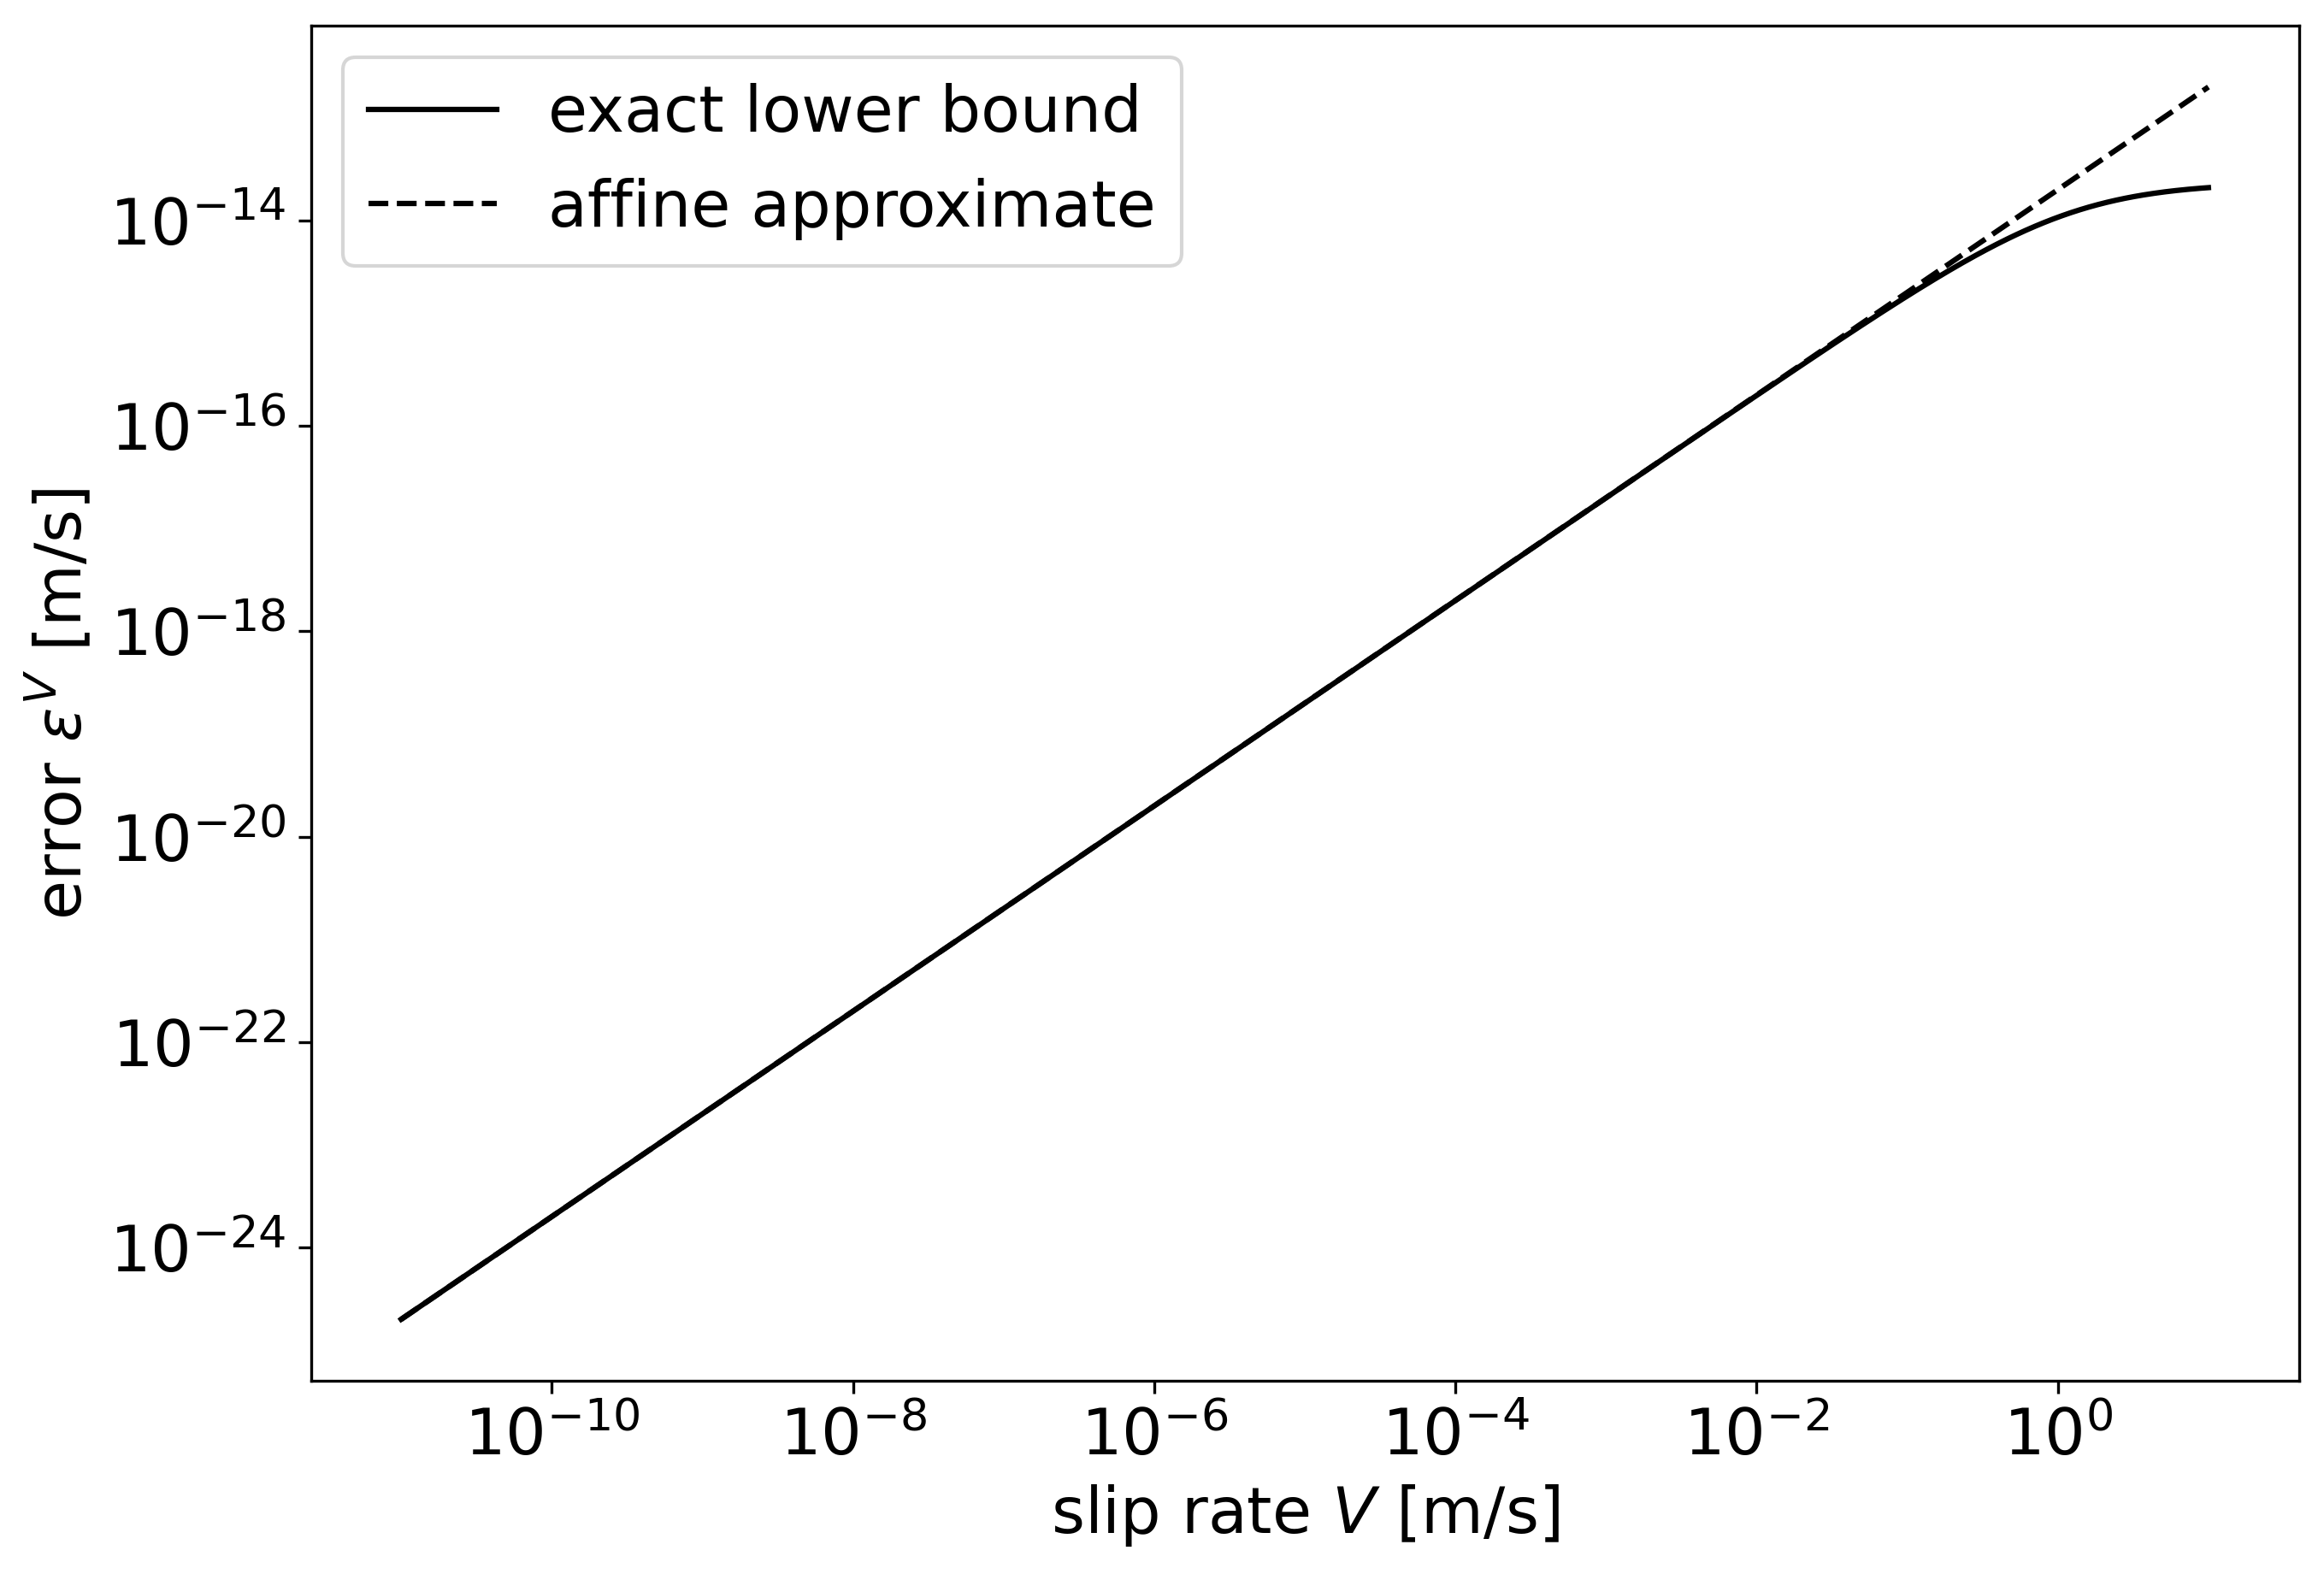
\includegraphics[width=0.5\textwidth]{images/ErrorRelationPSI_VAbsoluteRelative.png}
	\caption{Lower bound for the error in the slip rate $V$ compared to its linear approximate in function of the slip rate}
	\label{fig:LowerBoundErrorEstimateV}
\end{figure}

This section estimated a lower bound for the local truncation error of the different components $\varepsilon^S$, $\varepsilon^\psi$ and $\varepsilon^V$. This means that a tolerance below these values can never be achieved and are an absolute lower bound for $t_i^a$ and $t_i^r$. \\

However, the proposed tolerances are only of theoretical nature, as they assume that the error only stems from the iterative solver of the friction law. However, the time integration would most likely fail because numerical rounding errors or the sum of local truncation errors from the different RK stages have not been considered. Moreover, the error estimate itself is not exact, and, as already discussed in \autoref{ssec:QualityErrorEstimate_0D}, it tends to overestimate the local truncation error, which means that even if the error is within the tolerance, the algorithm would not consider it as such. If one wants to run the simulation with maximal accuracy, it is wise to use larger values than the here presented tolerances.


\section{Newton Iteration}
\label{ssec:ConvergenceNewtonIteration}
The Jacobian matrix is needed to apply implicit numerical methods to the SEAS problem. Unlike explicit methods, they evaluate the right hand side of the ODE with the current solution which is not known yet. To calculate the solution vector at a given timestep, a nonlinear algebraic equation of the form $\varphi(x) = 0$ needs to be solved where $x$ is the solution vector to be determined. The Newton method is often used to solve the equation because of its ease to implement and converges with second order around the solution. 

\begin{itemize}
	\item Calculate an initial guess $x_0$
	\item Repeat until tolerance is reached $\|\phi(x_n)\| < TOL$: 
	\begin{itemize}
		\item $x_{n+1} = x_n - J_\varphi^{-1}(\varphi(x_n)) \varphi(x_n)$
	\end{itemize} 
\end{itemize}

The matrix $J_\varphi^{-1}(f(x_n))$ is the Jacobi matrix of the function $\varphi$ evaluated at the point $x_n$. \\

\subsection{Convergence Properties}
Next, the convergence properties of the Newton iteration with the analytic Jacobian are investigated on the 1st order ODE formulation. For this, we solve one timestep of the implicit Euler method starting from the initial condition of the simulation. The function $\varphi$ and its Jacobian matrix are given by:
\begin{align}
\varphi(x) &= -x + x^{(0)} + h \Gamma(x) \\
J(x) &= -I + h J_\Gamma(x)
\end{align}
The vector $x$ contains both the components related to the slip $S$ and to the state variable $\psi$ and the right-hand side vector $\Gamma(x)$ contains their respective time derivative. The Jacobian of the proposed Newton iteration needs the Jacobian $J_\Gamma(x)$ of the right-hand side vector, of which the correctness is evaluated here. The success of the Newton iteration, thus to measure second-order convergence, also indicates the correctness of the Jacobian matrix. \\
Furthermore, the behavior of the analytic expression of the Jacobian is compared to the behavior of an iterative approximation of it. Broyden's method \cite{BroydenIteration} provides an enhancement of the Newton method which updates the Jacobian matrix at each iteration without the need of its analytical expression. The main difficulty lies in finding an appropriate initial guess to achieve fast convergence. 

\begin{itemize}
	\item Calculate the initial guesses $x_0$ and $J_0$
	\item Repeat until tolerance is reached $\|\varphi(x_n)\| < TOL$: 
	\begin{itemize}
		\item $\Delta x_n = x_n - x_{n-1}$ and $\Delta \varphi_n = \varphi(x_n) - \varphi(x_{n-1})$ 
		\item $J_n = J_{n-1} + \frac{\Delta \varphi_n - J_{n-1}\Delta x_n}{\|\Delta x_n\|^2} \Delta x_n^T$
		\item $x_{n+1} = x_n - J_n \varphi(x_n)$
	\end{itemize} 
\end{itemize}

The motivation behind this update scheme is to minimize the Frobenius norm $\|J_n~-~J_{n-1}\|_F$. As a matter of simplicity, the initial guess of the Jacobian is obtained with the analytical expression of it, even though its correctness has not yet been shown. Other initialization methods such as finite differences do not lead to convergence of the Broyden method. \\
The experiment has been performed on a symmetric, two-dimensional domain of varying size. The initial guesses for $x$ are obtained with one step of the explicit Euler method with a timestep of $h = 10^5$s. This timestep is large enough to obtain an error to the exact value at this time which requires several Newton iterations to be corrected but remains small enough to ensure that the Newton iteration converges at all. The evolution of the residual $\varphi(x_n)$ is shown in \autoref{fig:convergenceNewtonAndBroydenDifferentSizes}.

\begin{figure}[H]
	\centering
	\begin{subfigure}{0.45\textwidth}
		\centering
		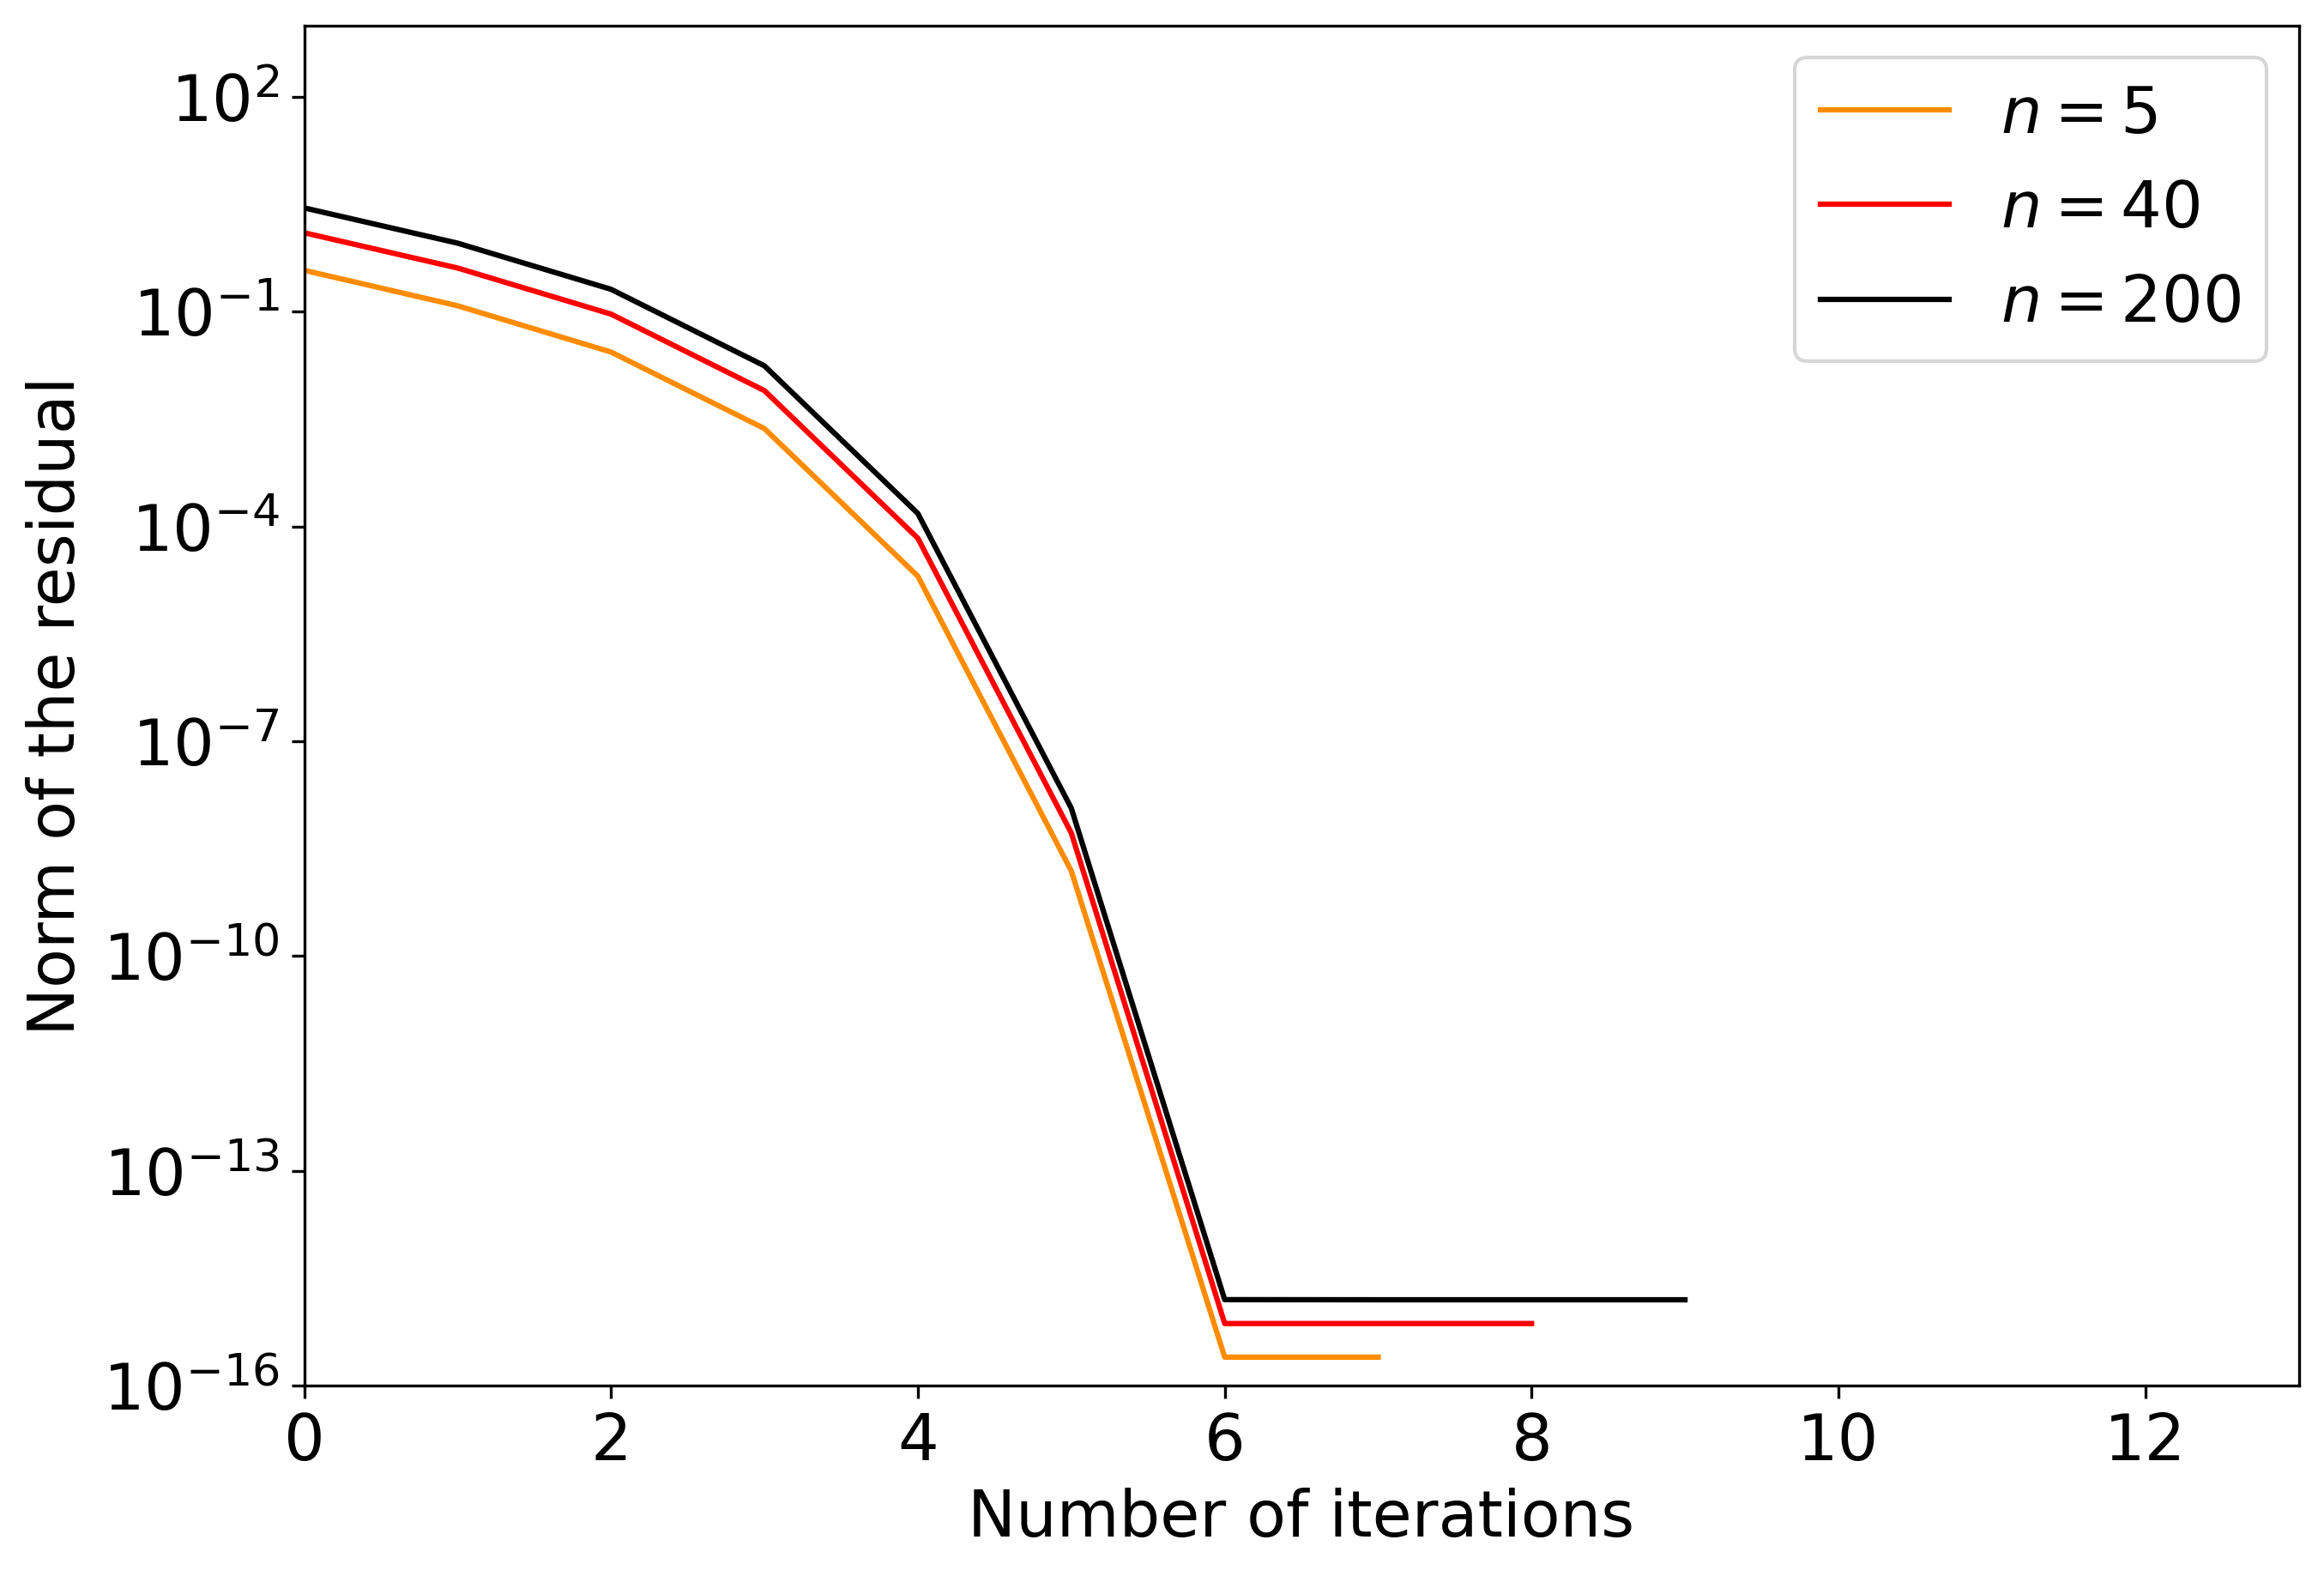
\includegraphics[width=1\textwidth]{images/NewtonIterationConvergenceDT1e5_DifferentSizes_Analytic.png}
		\subcaption{Direct iteration}
	\end{subfigure}
	\begin{subfigure}{0.45\textwidth}
		\centering
		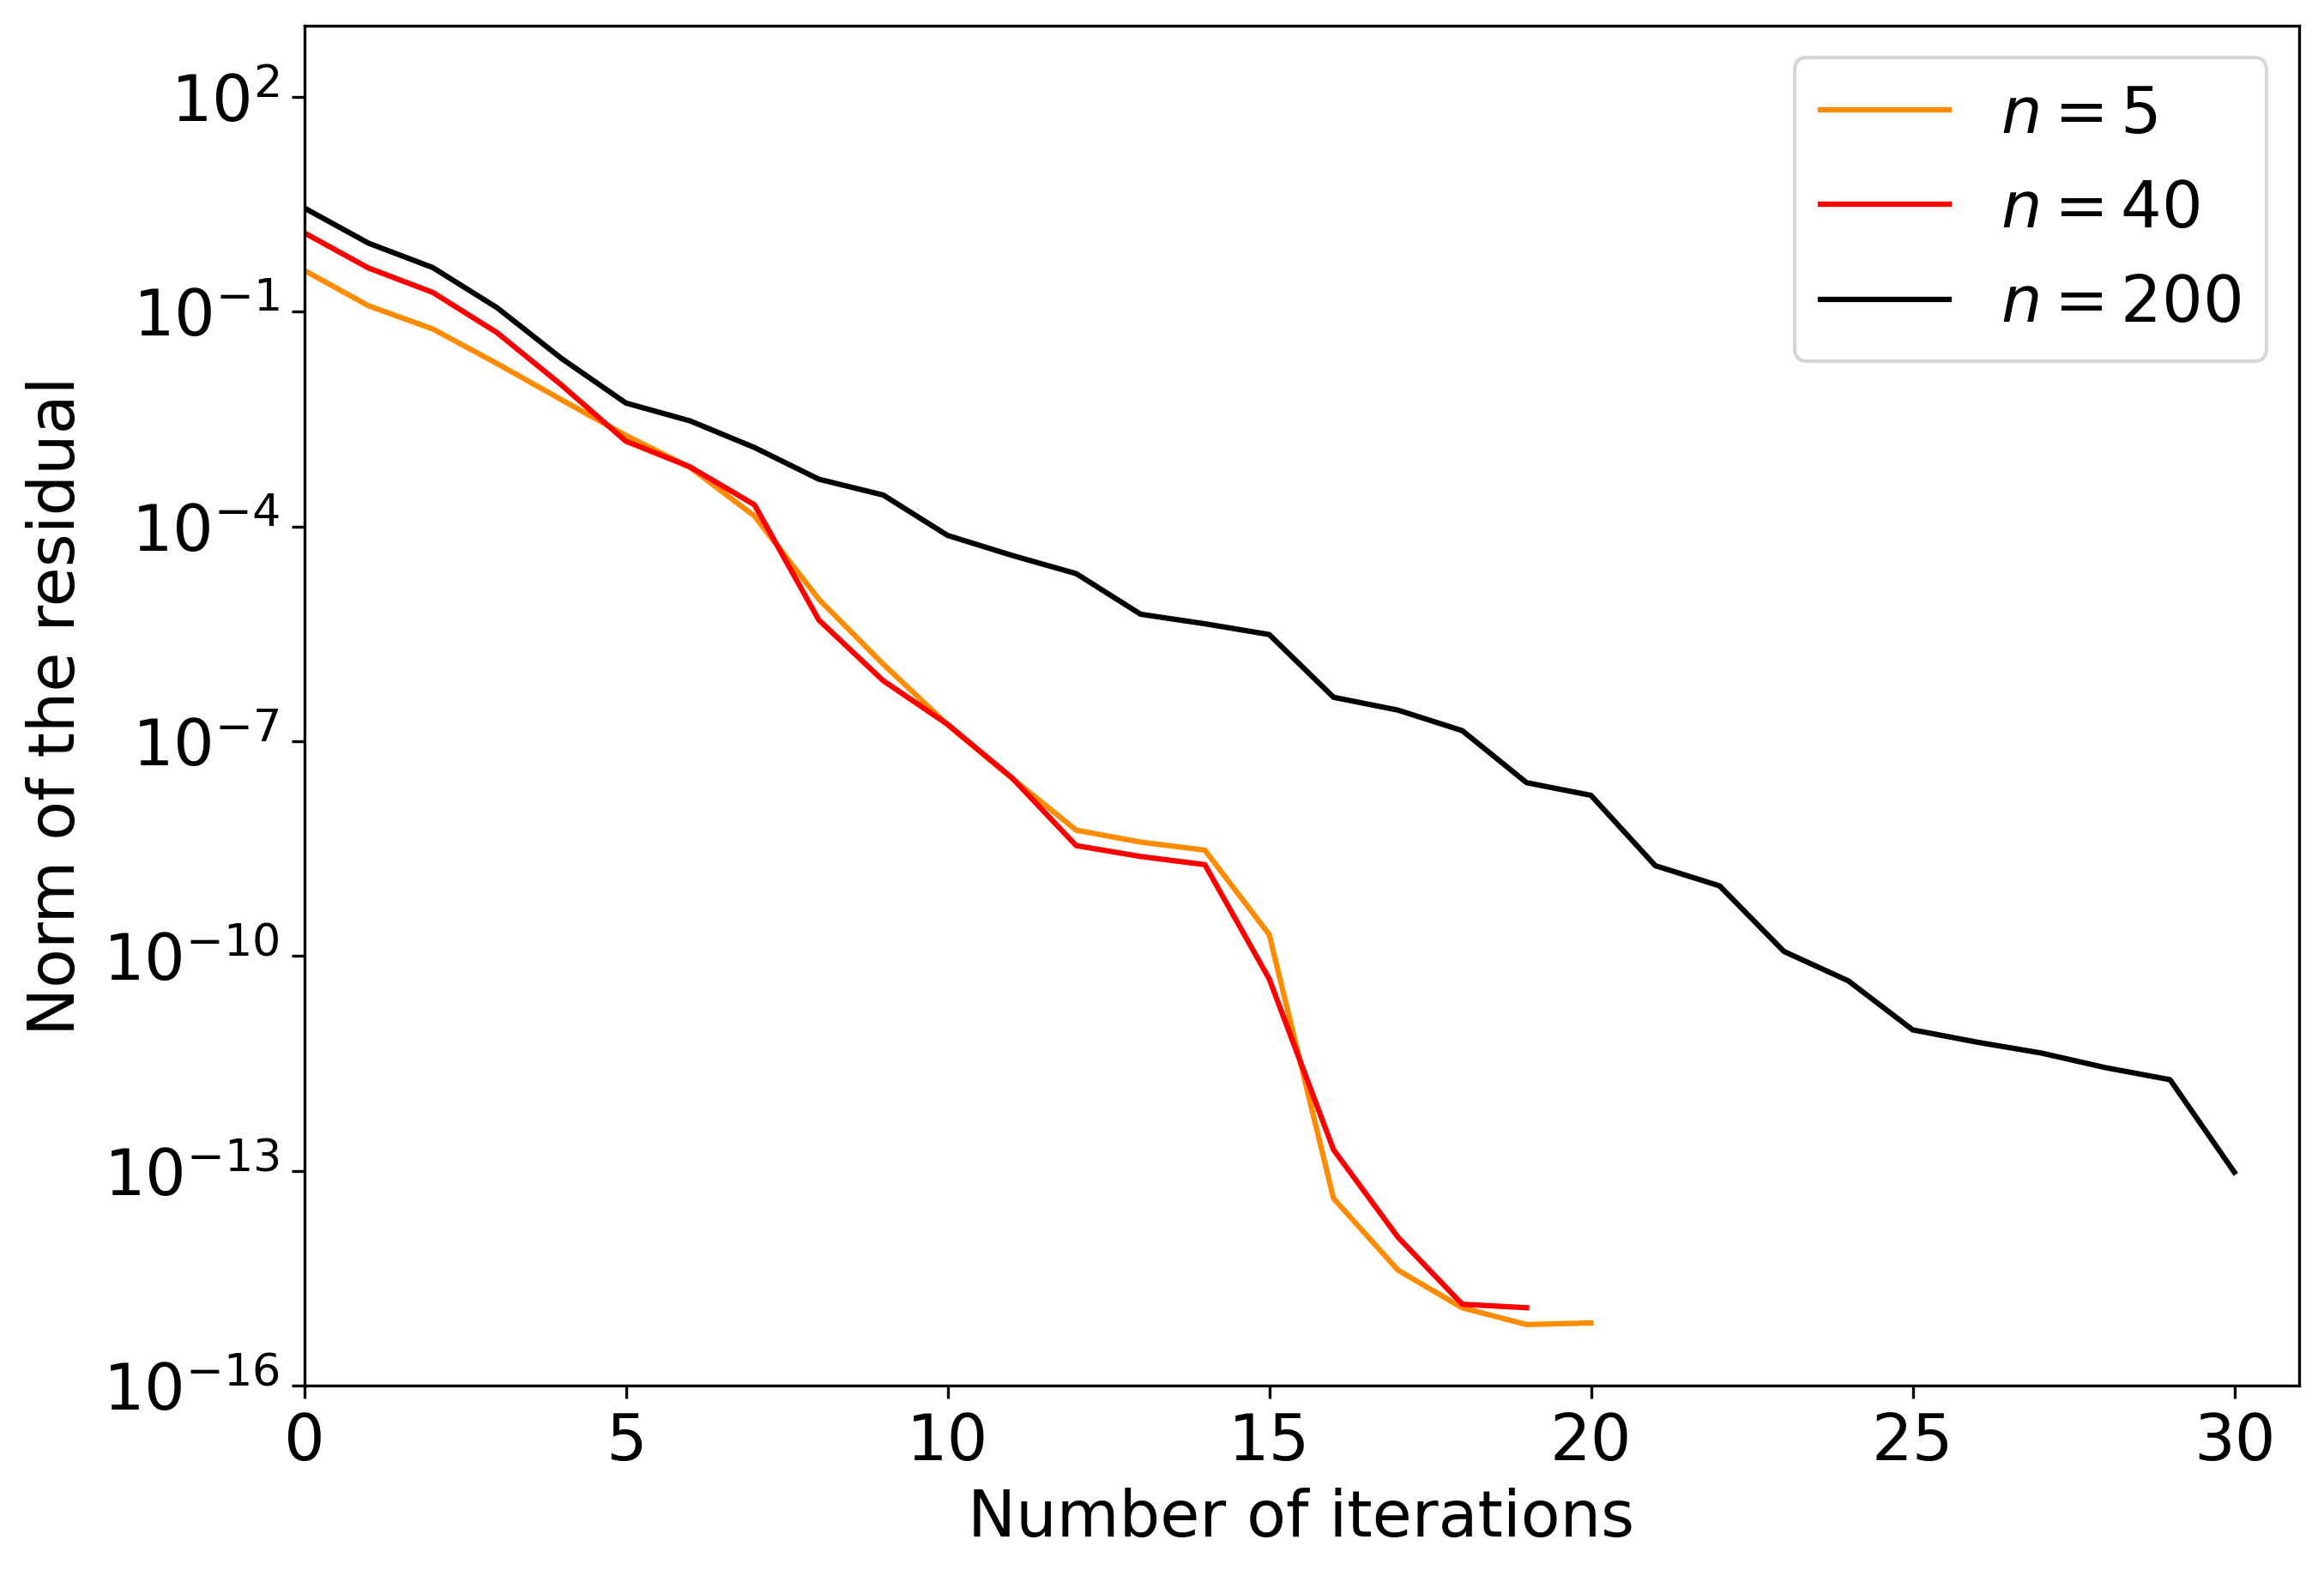
\includegraphics[width=1\textwidth]{images/NewtonIterationConvergenceDT1e5_DifferentSizes_Broyden.png}
		\subcaption{Broyden iteration}
	\end{subfigure}
	\caption{Evaluation of the L2 norm of the residual $\varphi(x_n)$ at each iteration of the Newton and Broyden methods for a timestep size of $h=10^5$s and for different problem sizes $n$}
	\label{fig:convergenceNewtonAndBroydenDifferentSizes}
\end{figure}

It can be immediately seen that the Newton method with an analytic expression of the Jacobian reaches the maximum reachable accuracy of about $10^{-15}$ much faster than if it was approximated with the Broyden method. The convergence rate even seems to be quadratic, as one would expect for the Newton iteration and the convergence is similarly fast for all tested domain sizes. The Broyden method on the other hand shows rather a linear convergence behavior, and the number of needed iterations increases with problem size. This makes the Broyden iteration particularly unsuitable for simulations on large domains. The approximated Jacobian matrix at the end of the Broyden iteration matches with high precision its analytic counterpart since the maximum relative difference among the entries is of the order of $10^{-5}$. \\
So far, it has been shown that the Newton iteration converges well for various domain sizes. The chosen timestep size $10^5$s is still small, as, in the aseismic slip, it may reach the order $10^7$s. \autoref{fig:convergenceNewtonAndBroydenDifferentTimeSteps} shows the norm of the residual for the timestep sizes $10^5$s, $10^6$s and $10^7$s. The direct iteration with the analytic Jacobian matrix always has a quadratic convergence, and the slightly higher number of iterations for large timesteps is essentially caused by the worse initial guess. In contrast, the Broyden iteration converges much slower if the timestep size increases. 
\begin{figure}[H]
	\centering
	\begin{subfigure}{0.45\textwidth}
		\centering
		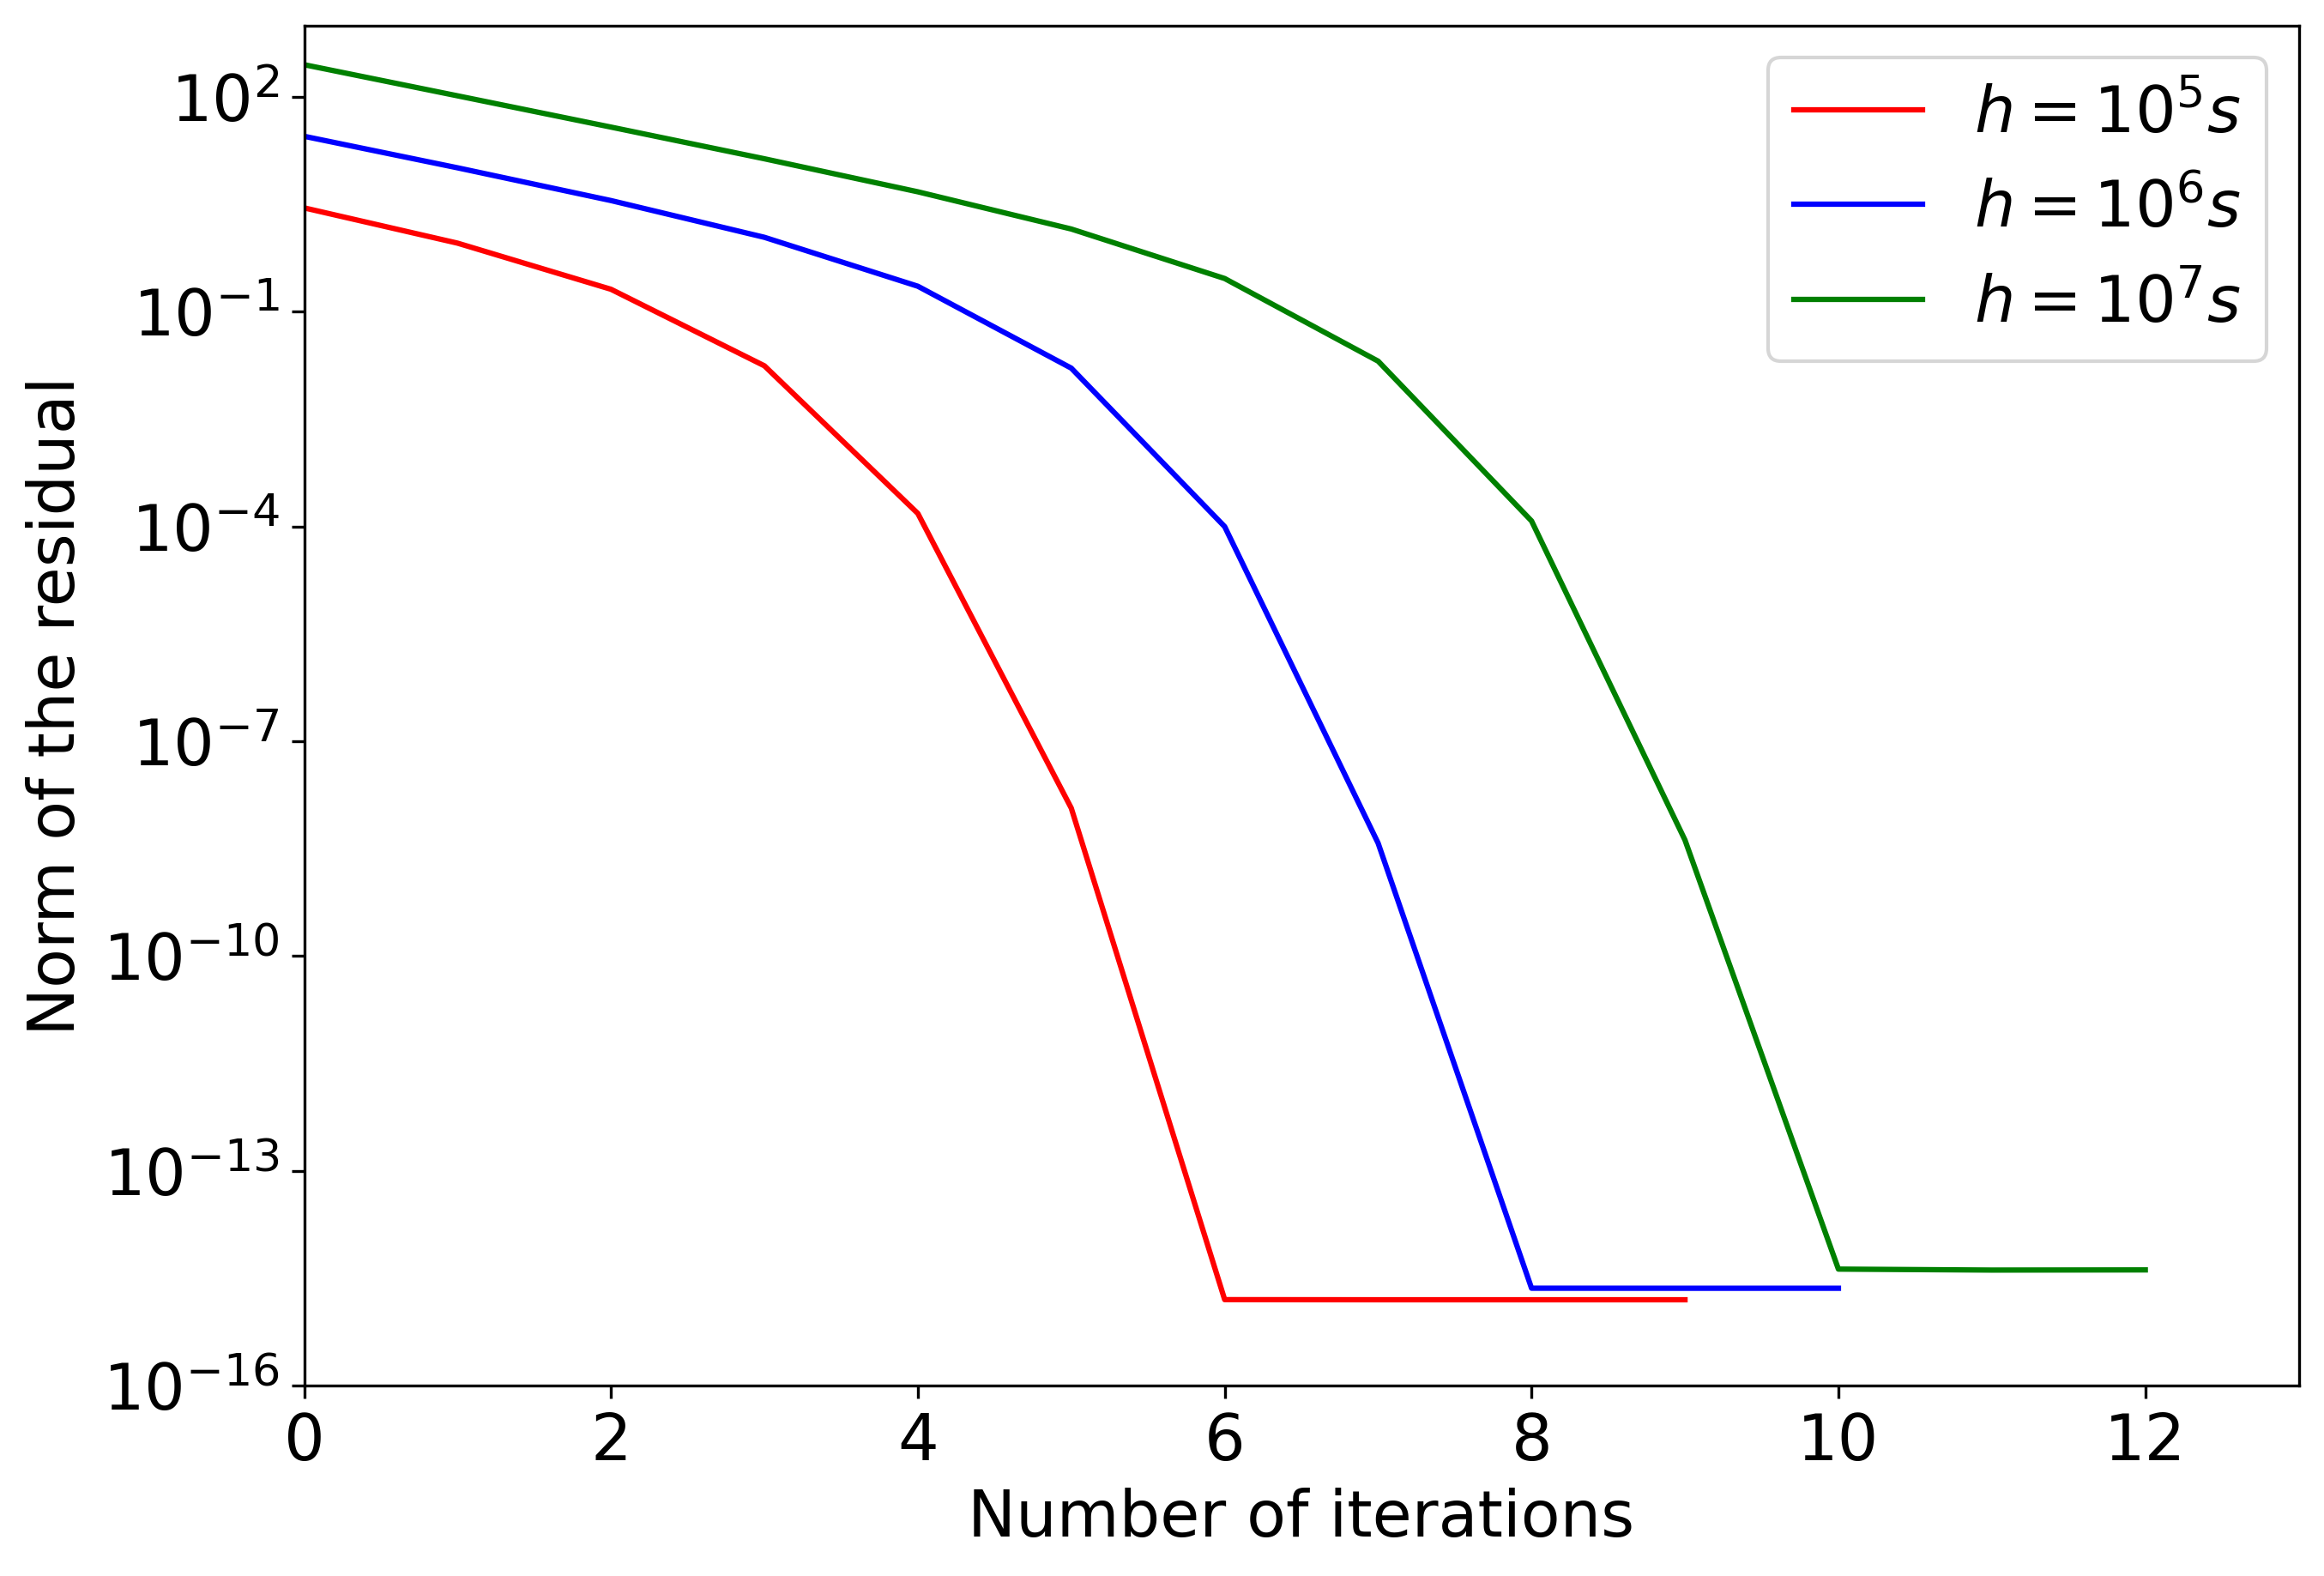
\includegraphics[width=1\textwidth]{images/NewtonIterationConvergence200Elements_DifferentDT_Analytic.png}
		\subcaption{Direct iteration}
	\end{subfigure}
	\begin{subfigure}{0.45\textwidth}
		\centering
		\includegraphics[width=1\textwidth]{images/NewtonIterationConvergence200Elements_DifferentDT_Broyden.png}
		\subcaption{Broyden iteration}
	\end{subfigure}
	\caption{Evaluation of the L2 norm of the residual $\varphi(x_n)$ at each iteration of the Newton and Broyden methods on a domain with 200 fault elements for different timestep sizes $h$}
	\label{fig:convergenceNewtonAndBroydenDifferentTimeSteps}
\end{figure}

It was shown that the Newton iteration with the analytic Jacobian has excellent convergence properties for any domain sizes and large timestep sizes. On the other hand, the alternative with a Broyden iteration, which approximates the Jacobian matrix along with the solution, converges only very slowly for large domains and large timesteps which is why this method is not suited to solve the problem. In practice, the  Newton iteration converges much faster because BDF schemes of higher order are used instead of the implicit Euler and the initial guess at the beginning of the iteration is obtained by extrapolating the previous solution vectors to the current simulation time. Usually, one Newton step is required to achieve the desired accuracy, which means two evaluations of the right-hand side function. \\

\subsection{Convergence issues with the compact DAE formulation}
The compact DAE formulation from \autoref{eq:DAE_compact_formulation_SEAS} shows a similar convergence behavior only during the aseismic slip. Whereas the method never diverges, the maximal achievable accuracy depends on the current timestep size, in a way that for very small timesteps, the residual in the Newton iterations does not go below some large value. Convergence to a non-optimal stationary point can be seen in \autoref{fig:convergenceIssuesCompactDAENewtonIterations}, which shows the infinity norm of the residual at each Newton step for different timestep sizes. The largest instance, of the order $10^7$, is representative of the aseismic slip after the first earthquake and the other samples have been taken in the initial phase of the second earthquake when the slip rate increases significantly and the timestep size decreases. \autoref{fig:convergenceIssuesCompactDAEMaxResidual_vs_dt} shows the maximum residual at the end of the Newton iteration in function of the current timestep size for all timesteps in the simulation. The locations of the samples in the first graph are highlighted by colored points. It can be seen that a large residual norm inversely depends on the timestep size. \\ 

\begin{figure}[H]
	\centering
	\begin{subfigure}[t]{0.32\textwidth}
		\centering
		\includegraphics[width=0.9\textwidth]{images/TANDEMConvergenceAnalysisCompactDAENewton_Size5.png}
		\subcaption{$\infty$-norm of the residual in the Newton iterations at different timestep sizes}
		\label{fig:convergenceIssuesCompactDAENewtonIterations}
\end{subfigure}
	\begin{subfigure}[t]{0.32\textwidth}
		\centering
		\includegraphics[width=1\textwidth]{images/TANDEMConvergenceAnalysisCompactDAEMaxResidual_Size5.png}
		\subcaption{Minimum achievable residual norms in function of the timestep size}
		\label{fig:convergenceIssuesCompactDAEMaxResidual_vs_dt}
	\end{subfigure}
	\begin{subfigure}[t]{0.32\textwidth}
		\centering
		\includegraphics[width=1\textwidth]{images/TANDEMConvergenceAnalysisCompactDAERatioInAddition_Size5.png}
		\subcaption{Minimum achievable residual norms in function of the maximal ratio between the additive terms in the Jacobian matrix}
		\label{fig:convergenceIssuesCompactDAEMaxResidual_vs_ratio}
	\end{subfigure}
	\caption{Convergence properties of the compact DAE formulation with the 4th order BDF method on a small domain with 5 fault elements}
\end{figure}
To obtain these results, the time integration itself has not been performed with the compact DAE formulation since it yields a poor accuracy, but rather with the 1st order ODE formulation using a classic adaptive RK4 scheme. At each timestep, the Newton iteration has been performed until the residual norm does not decrease anymore and the final result was discarded. Therefore, the solution vectors at the previous timesteps needed in the BDF method stem from the explicit RK4 time integration and thus slightly differ to the vectors in the time integration with the compact DAE formulation. In a discussion of the convergence this difference is not significant, since the convergence issues arise in either case. \\

The reason for this poor convergence can be found in the definition of the Jacobian matrix of the compact DAE formulation in \autoref{eq:Jacobian_compact_DAE}. As a quick reminder, the Jacobian matrix in the Newton iteration is obtained by $\mathbf{J} = \bm{\Phi}_x + \sigma \bm{\Phi}_{\dot{x}}$, where the shift $\sigma$ depends on the order $k$ of the BDF scheme and on the timestep sizes in  $k$ previous timesteps. The upper left block in the Jacobian is thus the sum of $\sigma\pdv{F}{V}$ and $\pdv{F}{S}$. The first partial derivative is of the magnitude $10^9$ in the aseismic slip and reaches values up to the order $10^{15}$ in an earthquake. On the other hand, the second summand takes values between $10^0$ and $10^2$. Since the former is a diagonal matrix, the sum only affects the diagonal elements. Since the timestep size does not change significantly after one timestep, it can be assumed that it is of the same order of magnitude as in the previous timestep. The shift $\sigma$ is then of the order $\sigma = \Theta\left(h_n^{-1}\right)$, where $h_n$ is current timestep size. In the aseismic slip, $\sigma$ is thus of the order $10^{-7}$ and can go as high as $10^3$ during an earthquake. In the worst case two terms of orders $10^{18}$ and $10^0$ have to be summed up, which cannot be represented anymore by a double-precision floating-point variable. The partial derivative $\pdv{F}{S}$ is therefore neglected in the Jacobian matrix during an earthquake and the friction law cannot be solved accurately anymore. \\
\autoref{fig:convergenceIssuesCompactDAEMaxResidual_vs_ratio} shows the maximum residual at the end of the Newton iteration in function of the ratio $\sigma\pdv{F}{V} / \pdv{F}{S}$ between the two problematic summands. As the ratio approaches and surpasses the machine precision of approximately $10^{16}$, the minimal achievable residual norm also increases. As a matter of fact, the convergence issues only appear in the residual components in $S$, for which the problematic summation occurs, whereas the residual components in $\psi$ remain at acceptable values below $10^{-12}$ throughout the simulation.
\\
In the last two graphs, a band with high accuracy and low timestep size appears at the bottom. These points correspond to the initial phase of the simulation, which is always launched in the aseismic slip phase with $h_0=0.1s$. Since the solution vector contains the initial value in these points, the Newton iteration directly converges with high precision. \\
This issue occurs only with the compact DAE formulation because the Jacobian matrices of the ODE formulations do not require any summations and in the extended DAE formulation, the two problematic terms $\pdv{F}{V}$ and $\pdv{f}{S}$ are located in different submatrices of $\bm{\Phi}_{\dot{x}}$ and $\bm{\Phi}_x$ and are thus never added to one another. \autoref{fig:convergenceIssuesExtendedDAEMaxResidual_vs_dt} shows the same dependency as in \autoref{fig:convergenceIssuesCompactDAEMaxResidual_vs_dt} for the extended DAE formulation. The norm of the residual at the end of the Newton iteration here does not depend on the timestep size and it varies between $10^{-12}$ and $10^{-15}$ throughout the simulation. Since both the slip and the state variable are of the order of $10^0$, the achieved tolerance is excellent and close to machine precision. \\
However, it seems that the best accuracy is only reached for large timesteps, whereas for very small timesteps, the Newton iteration only reached the "not the best but still very good" - accuracy of $10^{-12}$. In the definition of the Jacobian matrix for the extended DAE formulation in \autoref{eq:Jacobian_Newton_Iteration_extended_DAE}, there still is an addition between the shift $\sigma$ ($\sigma=1/h$ in the referred equation because it is related to the implicit Euler method) and the term $\pdv{G}{\psi}$. Since this last term is always of the order $10^{-7}$, the difference between the summands is not as extreme as for the compact formulation, but still noticeable for small timesteps, where $\sigma \approx 10^3$. Looking at \autoref{fig:convergenceIssuesExtendedDAEMaxResidual_vs_dt_onlyPSI}, the components of the residual vector relative to $\psi$ increase if the timestep size decreases. This is the same behavior as previously but on a much lower magnitude. Only in the earthquake phase, when timesteps below $0.1s$ are encountered, the residual in $\psi$ exceed the maximal precision $10^{-15}$ of the friction law and impacts the overall accuracy. 

\begin{figure}[H]
	\centering
	\begin{subfigure}[t]{0.45\textwidth}
	\centering
		\includegraphics[width=1\textwidth]{images/TANDEMConvergenceAnalysisExtendedDAEMaxResidual_Size5.png}
		\caption{Residual of all components}
		\label{fig:convergenceIssuesExtendedDAEMaxResidual_vs_dt}
	\end{subfigure} 
	\begin{subfigure}[t]{0.45\textwidth}
		\centering
		\includegraphics[width=1\textwidth]{images/TANDEMConvergenceAnalysisExtendedDAEMaxResidual_Size5_onlyPSI.png}
		\caption{Residual of the individual components $\psi$ and $S$}
		\label{fig:convergenceIssuesExtendedDAEMaxResidual_vs_dt_onlyPSI}
	\end{subfigure} 
	\caption{Minimum achievable residual norms in function of the timestep size for the extended DAE formulation with the 4th order BDF method on a small domain with 5 fault elements}
\end{figure}


In conclusion, the compact DAE formulation fails for the earthquake and can only be applied in the aseismic slip phase. Since the accuracy decreases along with the timestep size, the usual strategy to restart a step with a smaller timestep size if the nonlinear did not converge only leads to an even worse accuracy and is unsuitable.

\subsection{Stopping criterion}
\label{ssec:StoppingCriterionNewton}
The Newton iteration should be stopped when the norm of the residual becomes lower than some tolerance value or if the last Newton step could not decrease the norm further, as it happened for the compact DAE formulation. In this latter case, the Newton iteration is not rejected because the standard PETSc approach to reduce the timestep size cannot decrease the final residual error. Instead, a warning is printed to the terminal to notify the user that the Newton iteration could not reach the requested accuracy. If a $NaN$ value is encountered in the solution vector, or if the residual norm is larger than the initial norm, divergence is declared and PETSc is ordered to restart the current timestep with a smaller timestep size. \\
It makes sense to prescribe different tolerances for the components of the residual in $S$, $\psi$, $V$ or $f$ as for the time integration, since their magnitudes greatly differ. To ensure comparability with explicit methods, the friction law is always solved up to the maximum precision $\varepsilon_{max}$. The other tolerances are defined in a way that the local truncation errors in $\varepsilon^S$, $\varepsilon^\psi$ and $\varepsilon^V$ derived in \autoref{ssec:LowerBoundTimeTolerance} from $\varepsilon_{max}$ can be reached here. We use here $\varepsilon^S=4\cdot10^{-12}$, $\varepsilon^\psi=2\cdot10^{-14}$ and $\varepsilon^V=V_{min}\varepsilon_{max}/\sigma_n=2\cdot10^{-24}$. In the BDF scheme, the derivatives $\dot{x}$ are defined by the weighted sum of the component $x$ at the $k$ previous timesteps, so the error in $\dot{x}$ is driven by $C\varepsilon^x$, where the factor $C$ comes from the BDF coefficients and is minimal for large timesteps, where $C_{min}\approx10^{-7}$. The error of the functions $G$ and $H$ are approximated, as always, by a first order Taylor polynomial. Depending on the chosen formulation, the functional $\Phi$ contains a combination of the following four expressions, whose respective tolerances are limited by: 
\begin{align}
	\begin{cases}
	\Phi_S = V - \dot{S}  & (1) \\ 
	\Phi_\psi = G(\psi,V) - \dot{\psi} & (2)\\ 
	\Phi_F = F(S,\psi,V) & (3)\\ 
	\Phi_H = H(t,\psi,V) - \dot{V} & (4)
	\end{cases}
\end{align}
\begin{align}
	&\begin{cases}
	t_S < \left|C\varepsilon^S + \varepsilon^V\right| & (1)\\
	t_\psi < \left|C\varepsilon^\psi + \pdv{G}{\psi}\varepsilon^\psi + \pdv{G}{V}\varepsilon^V\right| & (2)\\
	t_F = \varepsilon_{max} & (3)\\
	t_V < \left|C\varepsilon^V + \pdv{H}{\psi}\varepsilon^\psi + \pdv{H}{V}\varepsilon^V\right| & (4)
	\end{cases} &&\Leftrightarrow&
	\begin{cases}
	t_S < 4\cdot10^{-19} & (1)\\ 
	t_\psi < 5\cdot10^{-21} & (2)\\
	t_F = 1\cdot10^{-12} & (3) \\
	t_V < 3\cdot10^{-22} & (4)
	\end{cases}
\end{align}
The 1st order ODE formulation needs the conditions (1) and (2), the extended DAE needs (1), (2) and (3), the compact DAE needs (2) and (3) and finally the second order ODE needs (1), (2) and (4). 

These values are only theoretical, and show how small the final residual norm in the Newton iteration should be to fit the time tolerances. Effectively, numerical rounding errors prevent reaching such small error values, as it has been shown for the compact DAE formulation, whose success in the earthquake is compromised for this reason. Reversely, this means that the implicit methods naturally cannot reach the same time accuracy as their explicit counterparts. By experience, the two working 1st order formulations can reach at most a final residual of $10^{-12}$ and the 2nd order ODE formulation reaches $10^{-16}$.


\subsection{Iterative solvers for the Newton step update}
In each Newton step, an expensive linear system has to be solved in $\mathcal{O}\left(n^3\right)$, which is the main bottleneck for simulations on large domains. To solve this issue, several iterative methods have been tested instead of the classical Gaussian elimination. PETSc comes along with a broad range of Krylov methods with even more preconditioners. Usable results could already be obtained with the simple Jacobi method \cite[p. 230]{IterativeSolutionMethods}. More advanced stationary iterative methods, such as Gauss-Seidel or SOR, were not used because their PETSc implementation skips the convergence test and always performs a fixed number of iterations. Further, a Krylov method has also been tested, the generalized minimal residual method (GMRES) \cite{GMRES}. In each iteration $k$, it minimizes the residual in the $k$th-Krylov subspace of the Jacobian matrix $J$ and returns the exact solution at the latest after $n$ steps, so the complexity is the same as for a direct method in the worst case. To improve its performance, both a Jacobi and a Gauss-Seidel preconditioner have been used. \\
The average number of iterations required to solve the linear system, as well as the impact of its accuracy on the Newton iteration and on the total number of timesteps are shown in Tables \ref{tab:compactODE_iterativeSolversJacobian}-\ref{tab:extendedODE_iterativeSolversJacobian} for all four formulations. The simulation length has been chosen such that exactly one earthquake happens, except for the compact DAE formulation, which generally fails to converge for small timesteps. For the ODE formulations, the iterative solver is directly applied to the Jacobian matrix as it appears in the Newton iteration and for the DAE formulations, the system is first reduced as described in \autoref{ssec:iterative_solver_Jacobian}. This is especially crucial for the extended DAE formulation since all methods fail to converge when directly applied to the Jacobian matrix. 

\subsubsection{1st order ODE formulation}
\begin{tabularx}{\textwidth}{|>{\centering\arraybackslash}m{0.3\textwidth} || c : c : c | c |}
	\hline
	& Jacobi & Jacobi-GMRES & GS-GMRES & LU \\ \hline\hline
	Average number of iterations per Newton step &  6.97  &    5.72   &    3.08  & -  \\ \hdashline
	Average number of Newton steps & 3.28  &     3.28    &   3.28  &     3.27 \\ \hdashline
	Average final Newton residual &   $1.07\cdot10^{-12}$  & $1.17\cdot10^{-12}$  & $1.33\cdot10^{-12}$  & $1.54\cdot10^{-12}$ \\ \hdashline
	Total number of timesteps & 4896  &      4906    &    4904    &    4901 \\
	\hline
	\caption{Quality of iterative solvers for the Jacobian system on a 5th-order BDF scheme with the 1st order ODE formulation on 101 fault elements for 250 years}
	\label{tab:compactODE_iterativeSolversJacobian}
\end{tabularx}

In the 1st order ODE formulation, the GMRES with a Gauss-Seidel preconditioner only needs an average of 3.08 iterations to solve the linear systems, as opposed to the Jacobi and Jacobi-GMRES methods with respectively 6.97 and 5.72 iterations. The quality of the Newton iteration and the total number of timesteps is very similar to the direct method for all three iterative methods, so the GS-GMRES method can be fully recommended for this formulation. 
\newpage 
\subsubsection{Extended DAE formulation}
\begin{tabularx}{\textwidth}{|>{\centering\arraybackslash}m{0.3\textwidth} || c : c : c | c |}
	\hline
	& Jacobi & Jacobi-GMRES & GS-GMRES & LU \\ \hline\hline
	Average number of iterations per Newton step &  7.48  &    5.11   &    2.77  & -  \\  \hdashline
	Average number of Newton steps & 4.07  &     4.82    &   4.51  &     4.23 \\  \hdashline
	Average final Newton residual &   $8.73\cdot10^{-12}$  & $1.17\cdot10^{-10}$  & $1.13\cdot10^{-10}$  & $4.53\cdot10^{-12}$ \\  \hdashline
	Total number of timesteps & 4920  &      4919    &    4919    &    4919 \\
	\hline
	\caption{Quality of iterative solvers for the Jacobian system on a 5th-order BDF scheme with the extended DAE formulation on 101 fault elements for 250 years}
	\label{tab:extendedDAE_iterativeSolversJacobian}
\end{tabularx}

In the extended DAE formulation, the three methods converge after a similar number of steps and again, the GS-GMRES method performs the best. However, both GMRES methods require slightly more Newton steps and only allow the Newton iteration to converge up to $10^{-10}$ and not $10^{-12}$ like the direct method or the Jacobi method. This reduced accuracy does not seem to impact the total number of timesteps, so the GS-GMRES can again be considered to be the best option, but there might be some simulation settings where the more accurate Jacobi method would be more appropriate.

\subsubsection{Compact DAE formulation}
\begin{tabularx}{\textwidth}{|>{\centering\arraybackslash}m{0.3\textwidth} || c : c : c | c |}
	\hline
	& Jacobi & Jacobi-GMRES & GS-GMRES & LU \\ \hline\hline
	Average number of iterations per Newton step &  10.85  &    6.58   &    3.45  & -  \\ \hdashline
	Average number of Newton steps & 3.98  &     4.01    &   3.97  &     3.97 \\ \hdashline
	Average final Newton residual &   $2.20\cdot10^{-11}$  & $2.22\cdot10^{-11}$  & $2.12\cdot10^{-11}$  & $2.04\cdot10^{-11}$ \\ \hdashline
	Total number of timesteps & 686  &      686    &    686    &    686 \\
	\hline
	\caption{Quality of iterative solvers for the Jacobian system on a 5th-order BDF scheme with the compact DAE formulation on 101 fault elements for 200 years}
	\label{tab:compactDAE_iterativeSolversJacobian}
\end{tabularx}
For the compact DAE formulation, the simulation was run only over 200 years, to avoid the earthquake for which this method does not converge. The GS-GMRES method performs again the best. Overall, more iterations are needed to converge than for its extended counterpart, albeit the comparison has only a limited significance because the latter went through an earthquake event, which is impossible for the former. 

\subsubsection{2nd order ODE formulation}
\begin{tabularx}{\textwidth}{|>{\centering\arraybackslash}m{0.3\textwidth} || c : c : c | c |}
		\hline
		& Jacobi & Jacobi-GMRES & GS-GMRES & LU \\ \hline\hline
		Average number of iterations per Newton step &  5.41  &    4.95   &    2.57  & -  \\ \hdashline
		Average number of Newton steps & 3.25  &     2.72    &   2.72  &     2.72 \\ \hdashline
		Average final Newton residual &   $1.91\cdot10^{-7}$  & $9.03\cdot10^{-16}$  & $7.85\cdot10^{-16}$  & $7.41\cdot10^{-16}$ \\ \hdashline
		Total number of timesteps & 11504  &      8308    &    8321    &    8306 \\
		 \hline
	\caption{Quality of iterative solvers for the Jacobian system on a 5th-order BDF scheme with the 2nd order ODE formulation on 101 fault elements for 250 years}
	\label{tab:extendedODE_iterativeSolversJacobian}
\end{tabularx}
Finally, in the 2nd order ODE formulation, there is a large difference between the Jacobi and the GMRES methods. The Jacobi method induces a much higher final residual in the Newton iteration, with a direct consequence on the total number of timesteps. On the other hand, with the GMRES methods, the simulation works as good as with a direct solver, and, as usual, the Gauss-Seidel preconditioner leads to fewer iterations than the Jacobi preconditioner. \\

In conclusion, iterative solvers are well-suited to update the Newton step. For all formulations, the GMRES method with a Gauss-Seidel preconditioner performs the best. The Jacobi preconditioner has the same impact on the overall performance of the simulation but requires more iterations to converge, so it does not bring any benefits. The Jacobi method has to be remembered as an alternative for the extended DAE formulation because the Newton iteration with GMRES is less accurate, which might impact the overall performance and accuracy under certain conditions. However, the Jacobi method should be avoided at any cost for the 2nd order ODE formulation, because it considerably affects the accuracy and performance of the simulation. 
	
\section{Data structure}
\label{sec:44mul4SEAS__Data}
\subsection{Block structure}
The solution vector is organized in a block structure that depends on the discretization of the DG scheme. The full 2D domain is discretized into triangular elements which each contains nodes at which the physical quantities are calculated. In our case, there are three nodes on each edge of an element, and this structure is preserved in the solution vectors and Jacobian matrices that are used in the time integration. Concretely, for one element, the values of a quantity at the three nodes are stored contiguously followed by the values of the next quantity. This structure is then repeated for all elements to form the entire solution vector. The order of the components is sketched in \autoref{fig:blockStructureScheme} for formulations that solve for the slip and the state variable. For the extended DAE and the 2nd order ODE formulations, the components of the slip rate $V_i$ are added elementwise after $\psi_i$.

\begin{figure}[H]
	\centering
	\includegraphics[width=0.9\textwidth]{images/blockStructure.png}
	\caption{Schematic representation of the components in the solution vector for the 1st order ODE and compact DAE formulations on three elements}
	\label{fig:blockStructureScheme}
\end{figure}

This block structure is also applied to the Jacobian matrices, such that they can be directly used in the Newton iteration. Setting up the matrix and the block matrix transformations in \autoref{ssec:iterative_solver_Jacobian} required thus arduous index operations.

\subsection{Memory requirements}
When the simulation will be scaled up to larger domains, memory requirements have to be taken into account. The most problematic term here will be the full matrix $\pdv{F}{S}$, whose size increases quadratically with the number of fault nodes. For example, a domain with $10^4$ fault elements and 3 nodes per fault requires, if all components are stored with double precision, 57.6GB memory just for the Jacobian matrix. Typically, such large simulations will be run on multiple cores once the code is parallelized, and the matrix is stored on multiple processors. The communication overhead to solve the Newton update will seriously hamper the performance, since there is no apparent pattern in $\pdv{F}{S}$ that could be efficiently used with parallel iterative solvers. The 1st order ODE with an explicit time integration is the only method that does not require setting up the dense matrix $\pdv{F}{S}$ and is not affected by these considerations. 



\chapter{Results}
\section{Evolution of Physical Quantities}
The simulation is run over a period of 250 years, in which one earthquake occurs on June 13th of the 195th year. This event can be clearly observed in \autoref{fig:timeEvolutionTANDEM_V} which depicts the maximum slip rate over time, which reaches $4.6m\cdot s^{-1}$ as opposed to an average of $1.0 \cdot 10^{-9}m\cdot s^{-1}$ in calm times. 
\begin{figure}[H]
    \centering
    \begin{subfigure}{0.32\textwidth}
     	\centering
    	\includegraphics[width=1\textwidth]{images/TANDEMcompareFormulationstimeEvolutionVall.png}
       	\subcaption{Full simulation time} 
    \end{subfigure} 
    \begin{subfigure}{0.32\textwidth}
    	\centering
    	\includegraphics[width=1\textwidth]{images/TANDEMcompareFormulationstimeEvolutionVsurroundings.png}
       	\subcaption{Year of the earthquake} 
    \end{subfigure}
    \begin{subfigure}{0.32\textwidth}
    	\centering
    	\includegraphics[width=1\textwidth]{images/TANDEMcompareFormulationstimeEvolutionVearthquake.png}
       	\subcaption{Evolution of the earthquake event} 
    \end{subfigure}
    \caption{Evolution of the maximal slip rate $V$ on the fault for different solvers on the symmetric two-dimensional BP1 problem with 200 elements on the fault}
    \label{fig:timeEvolutionTANDEM_V}
\end{figure}


\begin{figure}[H]
    \centering
    \begin{subfigure}{0.32\textwidth}
    	\centering
    	\includegraphics[width=1\textwidth]{images/TANDEMcompareFormulationstimeEvolutionDTall.png}
       	\subcaption{Full simulation time} 
    \end{subfigure}
    \begin{subfigure}{0.32\textwidth}
    	\centering
    	\includegraphics[width=1\textwidth]{images/TANDEMcompareFormulationstimeEvolutionDTsurroundings.png}
       	\subcaption{Year of the earthquake} 
    \end{subfigure}
    \begin{subfigure}{0.32\textwidth}
    	\centering
    	\includegraphics[width=1\textwidth]{images/TANDEMcompareFormulationstimeEvolutionDTearthquake.png}
       	\subcaption{Evolution of the earthquake event} 
    \end{subfigure}
    \caption{Evolution of the time step size $h$ for different solvers on the symmetric two-dimensional BP1 problem with 200 elements on the fault}
    \label{fig:timeEvolutionTANDEM_DT}
\end{figure}


\begin{figure}[H]
    \centering
    \begin{subfigure}{0.32\textwidth}
    	\centering
    	\includegraphics[width=1\textwidth]{images/TANDEMcompareFormulationstimeEvolutionRHSall.png}
       	\subcaption{Full simulation time} 
    \end{subfigure}
    \begin{subfigure}{0.32\textwidth}
    	\centering
    	\includegraphics[width=1\textwidth]{images/TANDEMcompareFormulationstimeEvolutionRHSsurroundings.png}
       	\subcaption{Year of the earthquake} 
    \end{subfigure}
    \begin{subfigure}{0.32\textwidth}
    	\centering
    	\includegraphics[width=1\textwidth]{images/TANDEMcompareFormulationstimeEvolutionRHSearthquake.png}
       	\subcaption{Evolution of the earthquake event} 
    \end{subfigure}
    \caption{Number of evaluations of the right hand side of the ODE in each time iteration for different solvers on the symmetric two-dimensional BP1 problem with 200 elements on the fault \newline
    \textbf{Legend:} \textcolor{red}{---} 1st order ODE formulation, \textcolor{blue}{---} 2nd order ODE formulation, \textcolor{green}{---} extended DAE formulation, \textcolor{yellow}{---} compact DAE formulation }
    \label{fig:timeEvolutionTANDEM_RHS}
\end{figure}


\section{Accuracy of the time integration}
\label{sec:Results_AccuracyTimeIntegration}
The discussion in \autoref{ssec:LowerBoundTimeTolerance} only tackled the question of the lowest allowable tolerances to reach as accurate results as possible. However, such strict tolerances may severely reduce the timestep size and by consequence the length of the simulation. For many applications, satisfactory results are already obtained for larger tolerances, and the aim of this section is to investigate it for SEAS. As there is no mathematical definition for \textit{satisfactory results} (unless convergence is the only requirement), we will run the simulation with the strictest possible tolerance described in the previous section and assess how the results deteriorate as the tolerances increase. Tolerances can be defined independently for the 
aseismic slip and for the earthquake, and will therefore be investigated separately. \\

The first set of experiments is performed with the 1st order ODE formulation on a domain with 101 fault elements to characterize the aseismic slip. The reference solution corresponds to the absolute tolerances $t_a^S =10^{-11}$ and $t_a^\psi =10^{-13}$, and this tolerance is kept in the earthquake phase for all simulation runs. In the simulated time of 300 years, two earthquakes occur after 204 and 270 years, and the accuracy is measured with the occurrence time of the first earthquake and with the period between the two events. The exact times are defined as the moment of the timestep, in which the highest maximum slip rate is reached. These metrics are appropriate, because the fundamental task of the aseismic slip is to build up stress until an earthquake is triggered, and an accurate simulation environment should detect the same earthquakes at the same times. The results are collected in \autoref{fig:tolerancesAseismicSlip_compactODE} for both the explicit, 5th order, Dormand-Prince RK method and the implicit, adaptive-order, BDF scheme.
\begin{figure}[H]
	\centering
	\begin{subfigure}[t]{0.32\textwidth}
		\centering
		\includegraphics[width=1\textwidth]{images/TANDEMcompactODEDifferentTolerancesSize101_AS_FirstEarthquakeTimeDiff.png}
		\subcaption{Time difference of the first earthquake} 
	\end{subfigure} 
	\begin{subfigure}[t]{0.32\textwidth}
		\centering
		\includegraphics[width=1\textwidth]{images/TANDEMcompactODEDifferentTolerancesSize101_AS_PeriodDiff.png}
		\subcaption{Difference of the period between both earthquakes} 
	\end{subfigure}
	\begin{subfigure}[t]{0.32\textwidth}
		\centering
		\includegraphics[width=1\textwidth]{images/TANDEMcompactODEDifferentTolerancesSize101_AS_DT.png}
		\subcaption{Geometric mean of the timestep size in the aseismic slip} 
	\end{subfigure}
	\caption{Difference of characteristic times to the reference solution for different tolerances in the aseismic slip phase for a domain with 101 fault elements with the 1st order ODE formulation}
	\label{fig:tolerancesAseismicSlip_compactODE}
\end{figure}

As expected, the accuracy of the predicted times worsens exponentially if the tolerance increases and the relationship. However, it appears that the implicit method deteriorates faster than the explicit,  With the RK method, all tolerances below $t_a^S<10^{-5}$m  and with BDF all below $t_a^S<10^{-7}$m allow to predict the earthquake up to an hour (=3600s) difference, which is very impressive considering the 200 years simulated time until it happens. It is much more accurate than the error induced by the DG scheme. Remember that in ??????? the earthquake got shifted by ?? years if the number of fault elements is doubled. It appears that the RK method fails if the tolerance exceeds $10^{-3}$m, which is not the case for the BDF method. Indeed, in the last few timesteps before the earthquake is triggered, the built-in iterative solver for the friction returns wrong values for $V$ until NaNs are encountered. In BDF, the residual of the Newton iteration diverges right away with wrong slip rates, and the timestep size is scaled down in time. However, at $t_a^S = 10^{-2}$m, which can only be reached with implicit methods, the times are off by $10^7$s $\approx 116$days and thus too inaccurate. \\

In the second experiment, the tolerance for the aseismic phase is kept constant and tolerances in the earthquake phase is progressively decreased. The simulation time is reduced to 250 years, such that only one earthquake occurs. The first quantity we look at is the overall maximum slip rate, that represents the intensity of the earthquake. Another interesting quantity is the increase in slip at the open surface, because this has a direct influence on the prediction of the subsequent earthquake: if the slip did not increase by much, the earthquake was not complete and the next happens earlier and inversely, if the earth moves too much, the next earthquake will be delayed. It is measured as the difference between the minimum slip at the end and the beginning of the simulation, which lie both in the aseismic phase surrounding the earthquake. The accuracy is thus estimated as a combination of the intensity and the geological changes in the earthquake. The results are found in \autoref{fig:tolerancesEarthquake_compactODE}, for the RK-DP and BDF schemes.

\begin{figure}[H]
	\centering
	\begin{subfigure}[t]{0.32\textwidth}
		\centering
		\includegraphics[width=1\textwidth]{images/TANDEMcompactODEDifferentTolerancesSize101_EQ_Vmax.png}
		\subcaption{Difference in the maximum slip rate} 
	\end{subfigure} 
	\begin{subfigure}[t]{0.32\textwidth}
		\centering
		\includegraphics[width=1\textwidth]{images/TANDEMcompactODEDifferentTolerancesSize101_EQ_Smin.png}
		\subcaption{Difference in the slip increase} 
	\end{subfigure}
	\begin{subfigure}[t]{0.32\textwidth}
		\centering
		\includegraphics[width=1\textwidth]{images/TANDEMcompactODEDifferentTolerancesSize101_EQ_DT.png}
		\subcaption{Geometric mean of the timestep size in the earthquake} 
	\end{subfigure}
	\caption{Difference of characteristic quantities to the reference solution for different tolerances in the earthquake for a domain with 101 fault elements with the 1st order ODE formulation}
	\label{fig:tolerancesEarthquake_compactODE}
\end{figure}
The slip induced by the earthquake is predicted in general with a very high accuracy. Stricter tolerances cannot ameliorate the results as the error for the slip stagnates around $10^{-8}$ with the RK method and around $10^{-7}$ with the BDF method. The fact that the explicit method is more exact than the implicit one is due to the condition of the Newton iteration and has already been discussed in \autoref{ssec:StoppingCriterionNewton}. Only after the RK method fails to converge at $t_a^S = 10^{-3}$, the accuracy begins to deteriorate exponentially with BDF, but even for the last tested tolerance, the difference to the reference solution is of the order of millimeters. Considering that in the reference solution, most of the simulated time is spent in the earthquake, it is strongly recommended to choose a much lower tolerance than for the aseismic slip. One big advantage of implicit methods here is that they return conclusive results even when explicit methods already failed. \\

In both earthquakes and aseismic phases, the timestep size increases logarithmically with the tolerance. With RK-DP, to increase the timestep size by one order of magnitude, the tolerance has to be four orders larger, which reflects the 4th order accuracy of the scheme. Simarly, for the BDF method, the ratio is six to one, which indicates that the order adapter chooses the BDF6 for most of the steps. However, prescribing a lower BDF order would not scale the timesteps faster up, as the adaptive-order finding already optimizes the time-step size. \\

The extended DAE formulation behaves essentially the same as the BDF method in the graphs above, and the compact DAE only for the aseismic slip, since it diverges in earthquakes. The 2nd order ODE formulation differs by the fact that it is driven by the state variable $\psi$ and the slip rate $V$, and the same set of experiments has been repeated, but for varying relative tolerances in $V$. The reference solution is set to $t_r^V=10^{-11}$, the error in the aseismic phase is shown in \autoref{fig:tolerancesAseismicSlip_extendedODE} and in the earthquake in \autoref{fig:tolerancesEarthquake_extendedODE}.
\begin{figure}[H]
	\centering
	\begin{subfigure}[t]{0.32\textwidth}
		\centering
		\includegraphics[width=1\textwidth]{images/TANDEMextendedODEDifferentTolerancesSize101_AS_FirstEarthquakeTimeDiff.png}
		\subcaption{Time difference of the first earthquake} 
	\end{subfigure} 
	\begin{subfigure}[t]{0.32\textwidth}
		\centering
		\includegraphics[width=1\textwidth]{images/TANDEMextendedODEDifferentTolerancesSize101_AS_PeriodDiff.png}
		\subcaption{Difference of the period between both earthquakes} 
	\end{subfigure}
	\begin{subfigure}[t]{0.32\textwidth}
		\centering
		\includegraphics[width=1\textwidth]{images/TANDEMextendedODEDifferentTolerancesSize101_AS_DT.png}
		\subcaption{Geometric mean of the timestep size in the aseismic slip} 
	\end{subfigure}
	\caption{Difference of characteristic times to the reference solution for different tolerances in the aseismic slip phase for a domain with 101 fault elements with the 2nd order ODE formulation}
	\label{fig:tolerancesAseismicSlip_extendedODE}
\end{figure}



\begin{figure}[H]
	\centering
	\begin{subfigure}[t]{0.32\textwidth}
		\centering
		\includegraphics[width=1\textwidth]{images/TANDEMextendedODEDifferentTolerancesSize101_EQ_Vmax.png}
		\subcaption{Difference in the maximum slip rate} 
	\end{subfigure} 
	\begin{subfigure}[t]{0.32\textwidth}
		\centering
		\includegraphics[width=1\textwidth]{images/TANDEMextendedODEDifferentTolerancesSize101_EQ_Smin.png}
		\subcaption{Difference in the slip increase} 
	\end{subfigure}
	\begin{subfigure}[t]{0.32\textwidth}
		\centering
		\includegraphics[width=1\textwidth]{images/TANDEMextendedODEDifferentTolerancesSize101_EQ_DT.png}
		\subcaption{Geometric mean of the timestep size in the earthquake} 
	\end{subfigure}
	\caption{Difference of characteristic quantities to the reference solution for different tolerances in the earthquake for a domain with 101 fault elements with the 2nd order ODE formulation}
	\label{fig:tolerancesEarthquake_extendedODE}
\end{figure}
Again, the accuracy increases with smaller tolerances, and the timestep size scales faster for the RK than for the BDF method. The RK method also fails if the tolerance is too large, but instead of NaNs, the slip rate just vanishes and the simulation finishes without detecting any earthquakes. Unlike the first order formulations, the second order ODE comes along with a much more accurate error estimate which is discussed in detail in the next section.




\section{Error estimation of the 2nd order ODE formulation}
Despite the lack of an analytic solution to the problem, this formulation of the problem offers a very powerful tool to evaluate the accuracy of the results. Since the slip rate is not calculated from the friction law anymore, it is not ensured that it is always equal to 0 up to numerical precision, as it was the case in the first order formulations of the SEAS problem. We could then evaluate the friction law at every timestep to assess the accuracy of the numerical integration. A large deviation from 0 of the absolute value of the friction law at a given timestep means that the integrator provides poor results. For a standard execution of the simulation with the second order formulation, this metric is not available, since the evaluation of $\tau$ in the friction law requires to solve the Poisson problem, and the big advantage of the new formulation is exactly not to solve this system. For the following graphs, The value of the friction law has been exceptionally calculated. \\

For the first set of pictures, a very small domain with 5 fault elements has been chosen to be able to observe the evolution of the quantities over a long period of time. The tolerances for the slip and the state variable have been fixed to $10^{-7}$. \autoref{fig:timeEvolution_2ndOrderODE_differentTolerances} shows the maximum value of the friction law for varying relative relative tolerances for $V$, and the absolute tolerance is fixed to 0. From the initial condition, the slip rate is calculated to fulfill the friction law up to numerical precision, at about $10^{-15}$. After some time steps, this high precision is lost, and at every earthquake event, the difference increases sharply. Overall, the logarithmic shape of the curves indicate a linear decrease of accuracy with time, It seems that, at every evaluation of the right-hand side function, for one given tolerance of $V$, a certain local truncation error is added to the residual of the friction law. At an earthquake, much more timesteps are required and the sum of the local truncation errors sum up to form an apparent sharp increase in the global error. For lower tolerances in $V$, the increase of the error at every evaluation is smaller the accuracy is higher. This hypothesis is confirmed by \autoref{fig:timeEvolution_LTE_2ndOrderODE_differentTolerances}, which shows the absolute change of the friction law per timestep. It can be considered somehow as an estimate for the local truncation error (LTE), as it describes how the error increases at each step. For a given tolerance in the slip rate, an upper bound for the LTE can be observed. During the earthquake, the LTE is actually much lower than in the aseismic slip. Only the high number of steps required for this event result in the apparent sharp increase of the total error. 

\begin{figure}[H]
	\centering
	\begin{subfigure}{0.45\textwidth}
		\centering
		\includegraphics[width=1\textwidth]{images/TANDEMtimeEvolutionFExtendedODEDifferentTolerances.png}
		\subcaption{Maximum absolute value of the friction law} 
		\label{fig:timeEvolution_2ndOrderODE_differentTolerances}
	\end{subfigure}
	\begin{subfigure}{0.45\textwidth}
		\centering
		\includegraphics[width=1\textwidth]{images/TANDEMtimeEvolutionFLTEExtendedODEDifferentTolerances.png}
		\subcaption{Absolute change of the friciton law per timestep, averaged over 50 timesteps} 
		\label{fig:timeEvolution_LTE_2ndOrderODE_differentTolerances}
	\end{subfigure}
	\caption{Evolution of the value of the friction law of the 2nd order formulation with 5 elements on the fault over 1000 years with varying relative tolerances in the slip rate $V$}
\end{figure}

The local truncation error seems to depend linearly on the tolerance for the slip rate, and a similar dependency is to be expected with respect to the tolerances of the slip $S$ and $\psi$, since these quantities are also required to evaluate the friction law. Next, we investigate whether other parameters, such as the spatial discretization, have an effect on the global error too. For a fixed relative tolerance for the slip of $10^{-7}$, the simulation has been executed for different spatial resolutions and the evolution of the friction law in each case is shown in \autoref{fig:timeEvolution_2ndOrderODE_differentSizes}. Since each fault elements contains three fault nodes, one has to multiply $n$ by three to obtain the total number of simulated fault nodes. At the beginning, all domain sizes have a similar accuracy, but after some earthquakes, it seems that the error in domains with higher resolution increases less fast. However, in \autoref{fig:timeEvolution_LTE_2ndOrderODE_differentSizes}, it is hard to distinguish separate upper bounds for the local truncation error with different domain sizes. The better performance of larger domains is rather due to the overall higher accuracy of simulations with higher resolutions and to a lower incidence of earthquakes, than due to a reduction of the LTE. 

\begin{figure}[H]
	\centering
	\begin{subfigure}{0.45\textwidth}
		\centering
		\includegraphics[width=1\textwidth]{images/TANDEMtimeEvolutionFExtendedODEDifferentSizes.png}
		\subcaption{Maximum absolute value of the friction law} 
		\label{fig:timeEvolution_2ndOrderODE_differentSizes}
	\end{subfigure}
	\begin{subfigure}{0.45\textwidth}
		\centering
		\includegraphics[width=1\textwidth]{images/TANDEMtimeEvolutionFLTEExtendedODEDifferentSizes.png}
		\subcaption{Absolute change of the friciton law per timestep, averaged over 50 timesteps} 
		\label{fig:timeEvolution_LTE_2ndOrderODE_differentSizes}
	\end{subfigure}
	\caption{Evolution of the value of the friction law of the 2nd order formulation over 400 years with varying domain sizes, where $n$ denotes the number of fault elements}
\end{figure}

Overall, the evaluation of the friction law is a suitable estimate for the global error in the system. Over the course of time, its value increases step wise at each earthquake, but overall linearly, which is due to a regular local truncation error. The main driver of the LTE is the tolerance for the slip rate $V$, which has been introduced to the system along with the second order ODE formulation. The upper bound for the LTE is proportional to the chosen tolerance.


\section{Time adaptivity of BDF methods}
\subsection{Quality of the error estimates}
Two error estimates have been introduced for the BDF methods. First, in a given time step, the BDF scheme is applied a second time with higher order and the difference between both available solutions at the timestep yields the error estimate. The second method bases on the derivatives of Lagrangian polynomials as described in \autoref{sssec:errorEstimateBDFLagrange}, and has the advantage to be much cheaper to evaluate, since it does not require to solve the system again. It has already been shown in \autoref{ssec:QualityErrorEstimate_0D} that for the 0D example, the first method gives a more accurate estimation of the local truncation error than the second method. Both methods tend to overestimate the error, which is for sure a safe behavior, but restrict the choice of the next timesteps. The aim of this section is to see, whether similar estimates can be observed for the current problem. \\
Since here no exact solution is available for the slip or the state variable (or the slip rate, if the solution vector has an extended size), the accuracy of the error estimate cannot be directly determined as previously. Instead, we assume that the actual error is inferior to the estimate, and that the embedded method is more accurate than Lagrangian polynomials. We would then expect that the timestep adapter chooses larger timesteps with the first method and finishes the program earlier. Exactly this can be observed in \autoref{fig:BDFOrders_Lagrange_vs_Embedded_compact_ODE} for the compact ODE formulation. As expected, the embedded method is faster than Lagrangian polynomials, because features, such as an increase or decrease of the timestep size happen increasingly earlier with the embedded method. Overall, fewer timesteps are required to reach a solution at a given time. However, the allowed timesteps are only slightly larger and the difference cannot be noticed on the logarithmic scale. Nonetheless, it is positive to remark that the same small features such as intermediate peaks are observed with both methods, which indicates that both error estimates recognize the same inconsistencies in the solution. 
\begin{figure}[H]
	\centering
	\includegraphics[width=0.8\textwidth]{images/TANDEMTimeAnalysisDifferentBDFOrdersEmbedded_vs_Lagrange_CompactODE_Size5.png}
	\caption{Comparison of the chosen timestep sizes with the Lagrangian polynomials (full line ---) and the embedded error estimate (dashed line - -) for different BDF orders on a domain with 5 fault elements and the compact ODE formulation with $\varepsilon^S_a = \varepsilon^{\psi}_a = 10^{-7}$ and $\varepsilon^S_r = \varepsilon^{\psi}_r = 0$ }
	\label{fig:BDFOrders_Lagrange_vs_Embedded_compact_ODE}
\end{figure}
Overall, the embedded method gives a more accurate error estimate than the Lagrangian polynomials, and allows for larger timestep sizes. However, the gain is only very small, as in average 2\% fewer timesteps are required in sum at the end of the simulation, and does not justify the use of the embedded higher order BDF method as error estimate, as it is twice as expensive. Actually, the order of the BDF method has a much higher influence on the total number of iterations, as it can be seen in this graph and will be discussed more in detail in the next section. 


\subsection{Effect of the order on the timestep size}
The order of the BDF method has a strong influence on the total number of required timesteps, as it can be clearly seen in \autoref{fig:BDFOrders_Lagrange_vs_Embedded_compact_ODE} from the previous section. The simulation can be roughly split into four sections: the evolution of the aseismic slip, with an approximately constant stepsize of the order of $h=10^7$s, the evolution of the earthquake at $h=10^{-2}$s and the transition between both phases, where the stepsize progressively increases or decreases. In addition to that, there is the initialization phase, in which the stepsize starts at $h=0.1$s to quickly reach the stepsize of the aseismic slip. \\
From \autoref{fig:BDFOrders_Lagrange_vs_Embedded_compact_ODE}, it seems that the stepsize of the constant evolution directly depends on the BDF order: a lower order leads to a smaller timestep and thus requires much more steps in total until the end of the aseismic slip or earthquake. The transition from the aseismic slip to the earthquake is a crucial section, because the sudden increase of the slip rate requires to rapidly scale down the timestep size. The end of the earthquake is less critical, as the slip rate drops relatively slowly which gives more scope to the stepsize to adapt to it, moreover the eventual too small stepsize there is not as problematic as a too high stepsize at the beginning of the earthquake. It is also interesting to look at the initialization phase, as there are no other constraints for a small stepsize but the limitations of the BDF scheme. \\
\autoref{fig:BDFOrders_compact_ODE_compare_initialization} shows exactly the increase at the beginning of the simulation for the BDF methods of order two to six and \autoref{fig:BDFOrders_compact_ODE_compare_begin_first_EQ} shows the transition from the aseismic slip to the first earthquake. To better contextualize the results, the graph for the explicit 4th order Runge-Kutta scheme with the same tolerances is also shown. In the initialization phase, the slope is in general steeper if a higher order method is used. One notable exception is the 6th order BDF scheme, which performs almost as bad as the 2nd order scheme. Unlike the other schemes, it does not increase smoothly but has regular steps, which indicates that the 6th order scheme is not as stable as the others. Overall, the increase is perfectly exponential for the schemes 2-5, and the factor by which the timestep size increases at each step is driven by the order of the method. Interestingly enough, in the very first timesteps,  the timestep size of the 2nd order scheme jumps by two orders of magnitude whereas the 5th and 6th order do not benefit at all from such a strong initial increase. At the transition from the aseismic slip to the earthquake phase, the timestep size decreases exponentially with the same pattern: a higher order scheme allows a stronger reduction of the timestep size from one step to the next. Now, the 6th order scheme is perfectly stable and has the steepest slope among all BDF methods. When compared to the explicit 4th order Runge-Kutta method, all BDF methods in both scenarios perform extremely bad. This is however not a reason to discard BDF methods as a whole, since they are much more flexible with respect to the defined tolerances, as it will be discussed in a later stage.

\begin{figure}[H]
	\centering
	\begin{subfigure}{0.45\textwidth}
		\centering
		\includegraphics[width=1\textwidth]{images/TANDEMTimeAnalysisDifferentBDFOrdersLagrange_CompactODE_Size5_Init.png}
		\subcaption{Maximum absolute value of the friction law} 
		\label{fig:BDFOrders_compact_ODE_compare_initialization}
	\end{subfigure}
	\begin{subfigure}{0.45\textwidth}
		\centering
		\includegraphics[width=1\textwidth]{images/TANDEMTimeAnalysisDifferentBDFOrdersLagrange_CompactODE_Size5_Begin1stEQ.png}
		\subcaption{Absolute change of the friciton law per timestep, averaged over 50 timesteps} 
		\label{fig:BDFOrders_compact_ODE_compare_begin_first_EQ}
	\end{subfigure}
	\caption{Evolution of the time step size for BDF schemes with different order at key points in the simulation on a domain with 5 fault elements and the compact ODE formulation with $\varepsilon^S_a = \varepsilon^{\psi}_a = 10^{-7}$ and $\varepsilon^S_r = \varepsilon^{\psi}_r = 0$ }
\end{figure}
Higher order BDF methods allow in general for higher stepsizes and are to be preferred over lower order methods. Since the costs of all BDF schemes are similar (they converge similarly fast and each Newton step always requires to solve one linear system), there is no strong reason to use a low order scheme here. Because of the stability issues with the 6th order scheme when the stepsize increases, the best performance can be expected from the 5th order scheme. There are some few cases where lower order methods perform better, such at the very beginning of the simulation. To take advantage of these peculiarities, and also to use the 6th order method if it is currently stable, the order of the BDF scheme can be adapted at each timestep as described in \autoref{sssec:adaptiveBDFOrder}. In this case, each step also calculates by how much the timestep size would change if one order higher or lower was used, and if a larger timestep can be reached, the order is changed for the next timestep. This has been implemented and the performance of the order-adaptive BDF scheme is shown in \autoref{fig:BDFOrders_compact_ODE_compare_adaptiveBDF}. It successfully uses the scheme with the largest allowable stepsize and finishes the simulation faster than any other methods. 


\begin{figure}[H]
	\centering
	\includegraphics[width=0.8\textwidth]{images/TANDEMTimeAnalysisDifferentBDFOrders_Lagrange_CompactODE_Size5_FULLTIME.png}
	\caption{Evolution of the time step size for the adaptive-order BDF method and for a selection of different fixed orders on a domain with 5 fault elements and the compact ODE formulation with $\varepsilon^S_a = \varepsilon^{\psi}_a = 10^{-7}$ and $\varepsilon^S_r = \varepsilon^{\psi}_r = 0$ }
	\label{fig:BDFOrders_compact_ODE_compare_adaptiveBDF}
\end{figure}


\section{Scalability}
The aim of this section is to investigate how the time integration scales with the problem size. To ensure comparability between the results, we set the tolerances such that the period between earthquakes and the slip increase are solved with similar accuracy, let us say to respectively $10^2$s and $10{-5}$m. From the analysis in \autoref{sec:Results_AccuracyTimeIntegration}, we can choose $t_a^S=10^{-8}$ and $t_a^S=10^{-5}$ for the aseismic and earthquake phases in first order formulations, and $t_r^V=10^{-8}$ and $t_r^V=10^{-7}$ in the second order ODE formulation. 

\begin{figure}[H]
	\centering
	\begin{subfigure}[b]{0.32\textwidth}
		\centering
		\includegraphics[width=1\textwidth]{images/TANDEM_averageNumberNewtonSteps.png}
		\subcaption{Average number of Newton steps per timestep} 
	\end{subfigure} 
	\begin{subfigure}[b]{0.32\textwidth}
		\centering
		\includegraphics[width=1.03\textwidth]{images/TANDEM_averageNumberKSPIteration.png}
		\subcaption{Average iteration number of the linear solver per Newton step} 
	\end{subfigure}
	\begin{subfigure}[b]{0.32\textwidth}
		\centering
		\includegraphics[width=1\textwidth]{images/TANDEM_averageNumberRHSEvaluations.png}
		\subcaption{Average number of RHS evaluations per timestep } 
	\end{subfigure}
	\caption{Number of iterations of the iterative solvers per timestep for the implicit formulations with different problem sizes. Note that each timestep includes one RHS evaluation before the Newton iteration}
	\label{fig:implicit_methods_scalabilty_iterations}
\end{figure}

\begin{figure}[H]
	\centering
	\begin{subfigure}[b]{0.32\textwidth}
		\centering
		\includegraphics[width=1\textwidth]{images/TANDEM_MeanTimeStepSize_AseismicPhase.png}
		\subcaption{Geometric mean of the timestep size in the aseismic phase}
	\end{subfigure}
	\begin{subfigure}[b]{0.32\textwidth}
		\centering \hspace{-0.75cm}
		\includegraphics[width=1.14\textwidth]{images/TANDEM_MeanTimeStepSize_EarthquakePhase.png}
		\subcaption{Geometric mean of the timestep size in the earthquake phase} 
	\end{subfigure}
	\begin{subfigure}[b]{0.32\textwidth}
		\centering
		\includegraphics[width=1\textwidth]{images/TANDEM_NumberTimeSteps_differentSizes.png}
		\subcaption{Total number of timesteps \\ \ }
	\end{subfigure}
	\caption{Behaviour of the timestep with different problem sizes.}
	\label{fig:scalabilty_timeStepSizes}
\end{figure}

\begin{figure}[H]
	\centering
	\begin{subfigure}[b]{0.32\textwidth}
		\centering
		\includegraphics[width=1\textwidth]{images/TANDEM_TimePerRHSEvaluation_differentSizes.png}
		\subcaption{Average execution time of each RHS evaluation}
	\end{subfigure}
	\begin{subfigure}[b]{0.32\textwidth}
		\centering \hspace{-0.75cm}
		\includegraphics[width=1.18\textwidth]{images/TANDEM_CPU_Time_intialization.png}
		\subcaption{Execution time of the initialization phase} 
	\end{subfigure}
	\begin{subfigure}[b]{0.32\textwidth}
		\centering
		\includegraphics[width=1\textwidth]{images/TANDEM_CPU_Time_solving.png}
		\subcaption{Execution time of the solving phase\\ \ } 
	\end{subfigure}
	\caption{Execution time of different sections of the simulation with different problem sizes.}
	\label{fig:scalabilty_executionTimes}
\end{figure}



\chapter{Extension to 3D}
\section{Elasticity Equation}
We now consider the original model from \autoref{ssec:GeneralSeasModel} with a three-dimensional domain and a two-dimensional fault. The antiplane shear assumption does not hold anymore and the Cauchy stress tensor $\mathbf{\sigma}$ has nonzero entries everywhere. This implies that the elasticity equation in \autoref{eq:GeneralElastostaticProblem} cannot be simplified to the Poisson problem anymore. \\

\subsection{Stress components at the fault}
In the general friction law \ref{eq:GeneralFrictionLaw}, the normal stress $\sigma_x$ acts as a factor to the friction coefficient and the shear stress $\tau$ contains two components $\tau_{xy}$ $\tau_{xz}$ in the direction of the slip rate. In terms of the Cauchy stress tensor, let us denote these three components by the vector $\mathbf{\bar{\sigma}}$. To calculate the Jacobian matrices of the system and to set up the second order ODE formulation, the partial derivatives with respect to both slip components $S_y$ and $S_z$ are required. Similarly to \autoref{sssec:Jacobian_ODE}, the partial derivatives $\pdv{u_{rs}}{S_{ln}}$, $\pdv{\mathbf{\bar{\sigma}}_{kp}}{u_{rs}}$ and $\pdv{\mathbf{\bar{\sigma}}_{kp}}{S_{ln}}$ have to be calculated to express the change in stress $\dv{\mathbf{\bar{\sigma}}_{kp}}{S_{ln}}$. Since the stress and the displacement $u$ acts in three dimensions over the indices $k$ and $r$, but the slip only in two over the index $n$, the final Jacobian is not a square matrix. \\
The term $\pdv{u_{sr}}{S_{ln}}$ is obtained by solving the discontinuous Galerkin problem with unit vectors instead of $S_{ln}$ without further source terms or boundary conditions. The stress $\mathbf{\hat{\sigma}}_{kp}$ at the quadrature points on one side of the fault and its derivative are calculated by:
\begin{align}
	\mathbf{\hat{\sigma}}_{pq} &= \lambda_q D_{lsq} u_{ls} n_{pq} + \mu_q \left(D_{ljq} u_{lp} n_{jq} + D_{lpq} u_{lj} n_{jq} \right) \\ \Leftrightarrow
	\pdv{\mathbf{\hat{\sigma}}_{pq}}{u_{rs}} &= \lambda_q D_{lsq} \pdv{u_{ls}}{u_{rs}} n_{pq} + \mu_q \left(D_{ljq} \pdv{u_{lp}}{u_{rs}} n_{jq} + D_{lpq} \pdv{u_{lj}}{u_{rs}} n_{jq} \right) \\ \Leftrightarrow
	\pdv{\mathbf{\hat{\sigma}}_{pq}}{u_{rs}} &= \lambda_q D_{rsq}  n_{pq} + \mu_q \left(D_{rjq} \delta_{ps} n_{jq} + D_{rpq} n_{sq} \right) \label{eq:intermediateStep7.3}
\end{align}
From \autoref{eq:intermediateStep7.3}, the term $\pdv{\mathbf{\bar{\sigma}}_{kp}}{u_{rs}}$ is obtained with the same further linear transformations that are applied from $\mathbf{\hat{\sigma}}$ to $\mathbf{\bar{\sigma}}$. Finally, the term $\pdv{\mathbf{\bar{\sigma}}_{kp}}{S_{ln}}$ is calculated in a similar fashion to \autoref{eq:JacobianDtauDS_Poisson}, under consideration of the correct dimensions. All together, the Jacobian matrix for the stress components with respect to the slip can be represented by the following block matrix.
\begin{equation}
	\label{eq:stressComponentsJacobian3D}
	\pdv{\mathbf{\bar{\sigma}}}{U}\pdv{U}{S}+ \pdv{\mathbf{\bar{\sigma}}}{S} = \dv{\mathbf{\bar{\sigma}}}{S} = \begin{pmatrix}
		\pdv{\sigma_x}{S_y} & \pdv{\sigma_x}{S_z}\\ 
		\pdv{\tau_{xy}}{S_y}  & \pdv{\tau_{xy}}{S_z} \\ 
		\pdv{\tau_{xz}}{S_y}  & \pdv{\tau_{xz}}{S_z}		
	\end{pmatrix}
\end{equation}
None of these entries depend on the current state of the system, the matrix can thus be pre-computed, as usual, in the initialization phase.

\subsection{Derivatives of the friction law}
The definition of the friction law in \autoref{eq:GeneralFrictionLaw} uses the absolute value of the shear stress and of the slip rate. As the components at the fault are two-dimensional, the euclidean norms of these quantities have to be computed before the friction law can be evaluated. This however complicates the Jacobian matrices $\pdv{F}{S}$ and $\pdv{F}{V}$, because the partial derivatives in both dimensions are now needed. We get:
\begin{equation}
	F(S,V,\psi) = \sqrt{\tau_{xy}^2 + \tau_{xz}^2} - \sigma_xf\left(\sqrt{V_y^2 + V_z^2},\psi\right) - \eta\sqrt{V_y^2 + V_z^2} 
\end{equation}
\begin{align}
	\label{eq:Jacobian_dF_dS_Elasticity3D}
	&\begin{cases}
		\pdv{F}{S_y} = \frac{1}{\norm{\tau}}\left(\tau_{xy}\pdv{\tau_{xy}}{S_y} + \tau_{xz}\pdv{\tau_{xz}}{S_y}\right) - \pdv{\sigma_x}{S_y}f(\norm{V},\psi) \\ 
		\pdv{F}{S_z} = \frac{1}{\norm{\tau}}\left(\tau_{xy}\pdv{\tau_{xy}}{S_z} + \tau_{xz}\pdv{\tau_{xz}}{S_z}\right) - \pdv{\sigma_x}{S_z}f(\norm{V},\psi) 
	\end{cases}
\end{align}
Unlike in the 2D problem, this term depends on the current state of the system and cannot be entirely precomputed. Luckily, it is obtained through linear transformations from the constant stress derivatives and the update is achieved in $\mathcal{O}\left(n^2\right)$. The vector of the slip rate is defined to always point in the direction of the shear stress on the fault. This motivates the introduction of a unit vector $u$ which always points in the current stress direction and whose components are:

\begin{align}
	u_y &= \frac{V_y}{\norm{V}} = \frac{\tau_{xy}}{\norm{\tau}} \\
	u_z &= \frac{V_z}{\norm{V}} = \frac{\tau_{xz}}{\norm{\tau}}
\end{align}

The unit vector gives the flexibility to be defined in the code either via the slip rate or the shear stress, preserving a consistent notation in the subsequent formulas. Further, the matrices $\mathbf{u_{y/z}}$ contain these components for each fault node on their diagonal. 
 
\section{Involved changes in the four formulations}
\subsection{First order ODE}
In the first order ODE formulation, the solution vector $x = (S_y, S_z, \psi)^T$ now contains two entries for the slip in $y$ and $z$ directions. The state variable $\psi$ remains of course a scalar quantity. The order of operations is not changed, thus at each evaluation of the right hand side, the absolute slip rate $\norm{V}$ is solved iteratively in the friction law with the norm of the shear stress. The $y$- and $z$-components of the slip rate are calculated by 
\begin{equation}
	\label{eq:update_V_3D}
	\begin{pmatrix}
		V_y \\ V_z
	\end{pmatrix} = \frac{\norm{V}}{\norm{\tau}} \begin{pmatrix}
													\tau_{xy} \\ \tau_{xz}
												 \end{pmatrix}
\end{equation}
and can be used for the right-hand side of the time derivatives $\dot{S}_y$ and $\dot{S}_z$. \\
For implicit methods, the Jacobian matrix has to be considerably adapted to split the derivatives with respect to the two fault dimensions. The Jacobians $\pdv{V_i}{S_j}$, where $i$ and $j$ stand for the two spatial directions $y$ and $z$ are calculated by derivating both sides of \autoref{eq:update_V_3D}.
\begin{align}
	\pdv{V_i}{S_j} =& \frac{\norm{V}}{\norm{\tau}}\pdv{\tau_{xi}}{S_j} + \frac{\pdv{\norm{V}}{S_j}\norm{\tau}-\norm{V}\pdv{\norm{\tau}}{S_j}}{\norm{\tau}^2}\tau_{xi} \nonumber\\ 
	=& \frac{\norm{V}}{\norm{\tau}}\pdv{\tau_{xi}}{S_j} + \mathbf{u_i}\left[-\left(\pdv{F}{V}\right)^{-1}\pdv{F}{S_j} - \frac{\norm{V}}{\norm{\tau}}\pdv{\sigma_{x}}{S_j}f(\norm{V},\psi)\right] 
	\label{eq:partial_V_S_Elasticity_3D}
\end{align}
where the Jacobian $\pdv{F}{V}$ has been previously calculated in \autoref{eq:partial_df_dV} and $\pdv{F}{S_j}$ is described in \autoref{eq:Jacobian_dF_dS_Elasticity3D}. Further, the derivative of $V_i$ with respect to the state variable and the derivatives of the ageing law $G$ are easily calculated as:
\begin{align}
	\label{eq:partial_dV_dpsi_elasticity_3D}
	\pdv{V_i}{\psi} &= \mathbf{u_i}\pdv{\norm{V}}{\psi} & &\text{using \autoref{eq:partial_V_psi}} \\
	\pdv{G}{S_j}    &= -\frac{b}{L}\left(\mathbf{u_y}\pdv{V_y}{S_j} + \mathbf{u_z}\pdv{V_z}{S_j}\right) & &\text{using \autoref{eq:partial_V_S_Elasticity_3D}} \\
	\pdv{G}{\psi}    &= -\frac{V_0}{L}e^{\frac{f_0 - \psi}{b}} -\frac{b}{L}\pdv{\norm{V}}{\psi} & & \text{using \autoref{eq:partial_V_psi}}
\end{align}

\subsection{Extended DAE}
For the extended DAE formulation, the solution vector $x = (S_y, S_z, \psi, V)^T$ also splits the slip in $y$ and $z$ components. The friction law in the last entry of the left-hand side function solves for the absolute value of the slip rate on each fault node. The separation in two components, needed for the derivatives $\dot{S}_y$ and $\dot{S}_z$ of the slip, are obtained from the direction of the shear stress as described in \autoref{eq:update_V_3D}. The Jacobian matrix contains the terms, with the shift $\sigma$ from the numerical scheme:
\begin{equation}
	\begin{pmatrix}
		\pdv{V_y}{S_y}-\sigma\mathbf{I} & \pdv{V_y}{S_z}                  & \mathbf{0}                      & \pdv{V_y}{V} \\
		\pdv{V_z}{S_y}                  & \pdv{V_z}{S_z}-\sigma\mathbf{I} & \mathbf{0}                      & \pdv{V_z}{V} \\ 
		\mathbf{0}                      & \mathbf{0}                      & \pdv{G}{\psi} -\sigma\mathbf{I} & \pdv{G}{V}   \\
		\pdv{F}{S_y}                    & \pdv{F}{S_z}                    & \pdv{F}{\psi}                   & \pdv{F}{V}
 	\end{pmatrix}
\end{equation}
The derivatives in the last column are all with respect to the absolute slip rate, and for the first two terms,  the derivatives are equal to the respective direction components $\pdv{V_y}{V} = u_y$ and $\pdv{V_z}{V} = u_z$. Further, the first two entries of the last row are exactly the matrices described in \autoref{eq:Jacobian_dF_dS_Elasticity3D}. Another novelty are the derivative terms $\pdv{V_i}{S_j}$ in the upper left corner. They are calculated the same way as in \autoref{eq:partial_V_S_Elasticity_3D}, but without the the derivative term with respect to the absolute slip rate:
\begin{equation}
	\pdv{V_i}{S_j} = \frac{\norm{V}}{\norm{\tau}}\left(\pdv{\tau_{xi}}{S_j} - \mathbf{u_i}\pdv{\sigma_x}{S_j}f(\norm{V}, \psi)\right)
\end{equation}
All other terms are scalar valued and are identical to the Jacobian of the two-dimensional Poisson problem derived in \autoref{sssec:Jacobian_DAE}. \\
The trick described in \autoref{ssec:iterative_solver_Jacobian} to effectively apply the iterative linear system solver on the dense subsystem and obtain the remaining entries by backward substitution is only of limited interest here, because the matrix now has six dense entries on three lines. Only the third block line may be eliminated.

The compact DAE formulation was not implemented with the 3D elasticity equation because of the observed convergence failure during earthquakes in the 2D scenario and its very similar behaviour to the extended DAE everywhere else. Moreover, it cannot be defined as straightforward in 3D, because the slip now has two components, but only one of them can be replaced by the friction law. 

\subsection{Second order ODE}
Finally, the most important task of this chapter is to get the best of all formulations, the second order ODE working in 3D. As the slip rate in the solution vector now directly stands for the derivative of the slip, we need both directional components and thus we have $x = (S_y, S_z, \psi, V_y, V_z)^T$. The same approach as in \autoref{eq:partial_V_S_Elasticity_3D} is followed to set up the time derivative $H$ of the slip rate. We get, for $i=y/z$:
\begin{align}
	H_i(\psi,V) &= \dv{V_i}{t} = \frac{\norm{V}}{\norm{\tau}}\dv{\tau_i}{t} + u_i\left(\dv{\norm{V}}{t} - \frac{\norm{V}}{\norm{\tau}}\dv{\norm{\tau}}{t}\right) \\
	&\text{with:}\qquad\begin{cases}
		\dv{\norm{V}}{t} = -\left(\dv{F}{V}\right)^{-1}\left[\pdv{\norm{\tau}}{t} - \pdv{\sigma_x}{t}f + \pdv{F}{S_j}\dv{S_j}{t} + \pdv{F}{\psi}\dv{\psi}{t} \right] \\
		\dv{\norm{\tau}}{t} = \pdv{\norm{\tau}}{t} + \pdv{\norm{\tau}}{S_j}\dv{S_j}{t} \\
		\dv{\tau_i}{t} = \pdv{\tau_i}{t} + \pdv{\tau_i}{S_j}\dv{S_j}{t}
	\end{cases}
\end{align}

Because the traction depends linearly on time, their partial derivatives can be precomputed once. Further, the partial derivatives of the slip rate in \autoref{eq:theLastLine} have already been stated in \autoref{eq:partial_V_S_Elasticity_3D} and \autoref{eq:partial_dV_dpsi_elasticity_3D}. As the value of the traction is not readily available but is needed in the ratio $\norm{V}/\norm{\tau}$, an alternative way to calculate this term is required. We know that, by definition, $\norm{\tau} = \sigma_x f + \eta\norm{V}$, and because the normal stress depends linearly of slip and time, we have $\sigma_x = \sigma_0 + \pdv{\sigma_x}{S_i}S_i + \pdv{\sigma_x}{t}t$. With this knowledge, first $\sigma$ and then $\norm{\tau}$ can be easily evaluated. Alternatively, it would have been possible to directly evaluate the shear stress components with the same method and calculate their norm $\norm{\tau}$. 

\section{Preliminary Results}
\subsection{Evolution of quantities}
Two test the 3D implementations, a simulation with 30 fault elements has been 


\subsection{Performance metrics}

\begin{table}[H]
	\centering 
	\begin{tabular}{ | c | c c c c |}
		\hline	
		& 1st order ODE 	& 1st order ODE 	& extended DAE  & 2nd order ODE  	\\ 
		& (RK)				& (BDF) 			&  (BDF) 		& (RK) 		  	 	\\ \hline
		CPU time in solving
		& 62978s 			& 34099s			& 33118s 		& 2587s			  	\\  
		Number of timesteps 	
		& 41361 		 	& 34118			 	& 34289			& 34289				\\\hline
	\end{tabular}
	\caption{Some performance results for the 3D simulation}
	\label{tab:performance_3D}
\end{table}








\begin{appendices}
	
	\chapter{Butcher tableaus of the used Runge-Kutta schemes}
	\label{apx:ButcherTableaus}
	
	\section{2nd order Bogacki-Shampine method}
	It is a 2nd order scheme with a 3rd order embedded method for the error estimate developped in 1989 \cite{RK-BogackiShampine}. It is well-suited if a rough error estimation is sufficient. The Butcher tableau reads:
	\begin{center}
		\begin{tabular}{c | c c c c}
			0 & & & & \\
			1/2 & 1/2 & & & \\
			3/4 & 0 & 3/4 & & \\
			1 & 2/9 & 1/3 & 4/9 & \\ \hline
			& 2/9 & 1/3 & 4/9 & 0 \\
			& 7/24 & 1/4 & 2/3 & 1/8
		\end{tabular}
	\end{center}
	
	\section{4th order Fehlberg method}
	It is a 4th order scheme with a 5th order embedded method for the error estimate developped in 1969 \cite{RK-Fehlberg}. It gives a more accurate error estimate than the RK-BS scheme and converges with 4th order. The Butcher tableau reads:
	
	\begin{center}
		\begin{tabular}{c | c c c c c c}
			0 & & & & & & \\
			1/4 & 1/4 & & & & & \\
			3/8 & 3/32 & 9/32 & & & &\\
			12/13 & 1932/2197 &	−7200/2197 & 7296/2197 & & & \\
			1 & 439/216 & −8 & 3680/513 & −845/4104 & & \\
			1/2 & −8/27 & 2 & −3544/2565 & 1859/4104 & −11/40 	& \\ \hline
			& 16/135 & 0 & 6656/12825 & 28561/56430 & −9/50 & 2/55 \\ 
			& 25/216 & 0 & 1408/2565 & 2197/4104 & −1/5 & 0 
		\end{tabular}
	\end{center}
	
	
	\section{5th order Dormand-Prince method}
	It is a 5th order scheme with a 4th order embedded method for the error estimate developped in 1969 \cite{RK-DormandPrince}. Unlike the Fehlberg scheme, it minimizes the error of the 5th order solution. The Butcher tableau reads:
	
	\begin{center}
	\begin{tabular}{c | c c c c c c c}
	0 & & & & & & & \\
	1/5 & 1/5 & & & & & & \\
	3/10 & 3/40 & 9/40 & & & & & \\
	4/5 & 44/45 & −56/15 & 32/9 & & & & \\
	8/9 & 19372/6561 & −25360/2187 & 64448/6561 & −212/729 & & & \\
	1 & 9017/3168 & −355/33 & 46732/5247 & 49/176 & −5103/18656 & & \\
	1 & 35/384 & 0 & 500/1113 & 125/192 & −2187/6784 & 11/84 & \\ \hline	
	& 35/384 & 0 & 500/1113 & 125/192 & −2187/6784 & 11/84 & 0 \\
	& 5179/57600 & 0 & 7571/16695 & 393/640 & −92097/339200 & 187/2100 & 1/40 
	\end{tabular}
	\end{center}

	
	\chapter{Alternative derivation of the BDF method}
	\label{apx:BDF_derivation_Taylor}
	The first order BDF-scheme corresponds to the backward Euler method in \autoref{eq:BDF_coeffs_1st_order}.
	\begin{equation}
	\label{eq:BDF_coeffs_1st_order}
	\psi_{n+1} = \psi_n + h_{n}f(\psi_{n+1},V_{n+1})
	\end{equation}
	Next, we try to derive the second order BDF-scheme. Because of the adaptive time-stepping, the traditional coefficients of the BDF2 scheme cannot be used, but will be dependent of the current and previous timestep sizes $h_{n+1}$ and $h_n$. To find these coefficients, the Taylor polynomials of $\psi_n$ and $\psi_{n+1}$ are evaluated with respect to the unknown $\psi_{n+2}$. 
	\begin{align}
	\label{eq:taylor-polynomialBDF1(1)}
	\psi_{n} &= \psi_{n+2} - (h_{n} + h_{n+1})\frac{d\psi_{n+2}}{dt} + \frac{(h_{n} + h_{n+1})^2}{2}\frac{d^2\psi_{n+2}}{dt^2} + \mathcal{O}\left((h_{n} + h_{n+1})^3\right) \\
	\label{eq:taylor-polynomialBDF1(2)}
	\psi_{n+1} &= \psi_{n+2} - h_{n+1}\frac{d\psi_{n+2}}{dt} + \frac{h_{n+1}^2}{2}\frac{d^2\psi_{n+2}}{dt^2} + \mathcal{O}\left(h_{n+1}^3\right)
	\end{align}
	The idea is to add equations (\ref{eq:taylor-polynomialBDF1(1)}) and (\ref{eq:taylor-polynomialBDF1(2)}), where the latter is multiplied by a factor $\alpha$ in a way that the second-derivative term drops. The addition of the two Taylor-expansions yields: 
	\begin{equation}
	\psi_{n} + \alpha \psi_{n+1} = (1+\alpha)\psi_{n+2} - \left(h_{n} + (1+\alpha)h_{n+1}\right)\frac{d\psi_{n+2}}{dt} + \frac{(h_{n} + h_{n+1})^2+\alpha h_{n+1}^2}{2}\frac{d^2\psi_{n+2}}{dt^2} + \mathcal{O}\left(h^3\right) \\
	\end{equation}
	By the choice of $\alpha$ in \autoref{eq:alpha}, the coefficient in front of the second time derivative of $\psi_{n+2}$ vanishes and the second order time adaptive BDF method is given by: \autoref{eq:BDF_coeffs_2nd_order}. 
	\begin{align}
	\label{eq:alpha}
	\alpha &= -\left(\frac{h_n}{h_{n+1}}\right)^2 - 2\frac{h_n}{h_{n+1}} - 1 \\
	\label{eq:BDF_coeffs_2nd_order}
	\psi_n + \alpha \psi_{n+1} -(1+\alpha)\psi_{n+2} &= -\left(h_n + (1+\alpha)h_{n+1}\right)f(\psi_{n+2}, V_{n+2})
	\end{align}
	Analogously, the time-adapative third-order BDF3 scheme is given with the coefficients: 
	\begin{align}
	\alpha &= -\frac{\left(h_n+h_{n+1}\right)\left(h_n+h_{n+1}+h_{n+2}\right)^2}
	{h_{n+1}\left(h_{n+1}+h_{n+2}\right)^2} \\
	\beta &= \frac{h_n\left(h_n+h_{n+1}+h_{n+2}\right)^2}
	{h_{n}^2h_{n+1}}
	\end{align}
	\begin{equation}
	\label{eq:BDF_coeffs_3rd_order}
	\psi_n + \alpha \psi_{n+1} + \beta \psi_{n+2} -(1+\alpha+\beta)\psi_{n+3} = \left(h_n + (1+\alpha)h_{n+1} + (1+\alpha+\beta)h_{n+2}\right)f(\psi_{n+3},V_{n+3})
	\end{equation}
	
	\chapter{Reduced Jacobian system for the extended DAE formulation}
	\label{apx:ReducedJacobianExtendedDAE}
	To efficiently apply iterative solvers for the extended DAE formulation, a blockwise Gaussian-elimination on the sparse components of the Jacobian matrix can be calculated such that the iterative solvers are only applied on a dense subsystem. For a general 2D problem, the Jacobian system takes the form: 
	\begin{equation}
		\begin{pmatrix}
			\mathbf{J}_{11} & \mathbf{0}      & \mathbf{J}_{13} \\
			\mathbf{0}        & \mathbf{J}_{22} & \mathbf{J}_{23}   \\
			\mathbf{B}      & \mathbf{J}_{32} & \mathbf{J}_{33}   \\
		\end{pmatrix}\begin{pmatrix}
		   				x_1 \\ x_2 \\ x_3 
					 \end{pmatrix} = \begin{pmatrix}
										 b_1 \\ b_2 \\ b_3 
									 \end{pmatrix}
 	\end{equation}
 	The sparse components are in the submatrices $\mathbf{J}_{ij}$ and the dense parts are in $\mathbf{B}$. After the Gaussian elimination, we get:
	\begin{align}
	\begin{pmatrix}
		\mathbf{B} - \mathbf{J}_{33}\mathbf{J}_{13}^{-1}\mathbf{J}_{11} + \mathbf{J}_{32}\mathbf{J}_{22}^{-1}\mathbf{J}_{23}\mathbf{J}_{13}^{-1}\mathbf{J}_{11} & \mathbf{0} & \mathbf{0} \\
		-\mathbf{J}_{23}\mathbf{J}_{13}^{-1}\mathbf{J}_{11} & \mathbf{J}_{22} & \mathbf{0}   \\
		\mathbf{J}_{11} & \mathbf{0} & \mathbf{J}_{13} \\
	\end{pmatrix}\begin{pmatrix}
					x_1 \\ x_2 \\ x_3 
			     \end{pmatrix} =  \qquad\qquad\qquad\qquad\nonumber \\ \qquad\qquad\qquad\qquad\qquad\qquad\qquad
	\begin{pmatrix}
		b_3 - \mathbf{J}_{33}\mathbf{J}_{13}^{-1}b_1 - \mathbf{J}_{32}\mathbf{J}_{22}^{-1}\left(b_2 - \mathbf{J}_{23}\mathbf{J}_{13}^{-1}b_1\right) 
		\\ b_2 - \mathbf{J}_{23}\mathbf{J}_{13}^{-1}b_1 
		\\ b_1 
   	 \end{pmatrix}
	\end{align}
 The upper-left block form the reduced system which is solved iteratively. The other solution components are then calculated by an easy backward substitution.

\end{appendices}

\bibliographystyle{alpha}
\bibliography{literature.bib}

\end{document}
